\documentclass[a4paper]{article}
\usepackage[utf8]{inputenc}




\title{Misura del coefficiente di restituzione\\ analisi dati}
\author{Ali Matteo,\\Broggi Diana, Cantarini Giulia}
\date{ }

\usepackage{tabularx}
\usepackage{natbib}
\usepackage{graphicx}
%\usepackage[demo]{graphicx}
%\usepackage{subfig}
%\usepackage[margin=1.0in]{geometry}


\usepackage{subcaption}
\usepackage{tikz}

\usepackage{amsmath, amsthm}

\usepackage{mathrsfs}

\usepackage{pgfplots}
%\pgfplotsset{width=4cm,compat=1.9}

\theoremstyle{definition}
\newtheorem{rich}{richiamo matematico}[section]





%roba che crea comando per centrare immagine dentro immagine piu grande
%https://tex.stackexchange.com/a/308286
\newlength{\imagew}
\newlength{\imageh}
\newlength{\legendw}
\newlength{\legendh}
\newlength{\legendx}
\newlength{\legendy}
\newcommand{\graphicswithlegend}[6]{
	\setlength{\imagew}{#1}
	\settoheight{\imageh}{\includegraphics[width=\imagew]{#2}}
	
	\setlength{\legendw}{#3\imagew}
	\settoheight{\legendh}{\includegraphics[width=\legendw]{#4}}
	
	\setlength{\legendx}{\imagew}
	\addtolength{\legendx}{-\legendw}
	\addtolength{\legendx}{-#5\imagew}
	
	\setlength{\legendy}{\imageh}
	\addtolength{\legendy}{-\legendh}
	\addtolength{\legendy}{-#6\imageh}
	
	\includegraphics[width=\imagew]{#2}%
	\llap{
		\hspace{-\the\legendx}
		\raisebox{\legendy}{\includegraphics[width=\legendw]{#4}}
		\hspace{\the\legendx}
	}
}



\begin{document}
	\pagenumbering{arabic}
	\maketitle
		\section*{Pallina da ping pong su parquet}
	\subsubsection*{metodo 1}
	Tabelle della altezza massima raggiunta dopo il primo rimbalzo in cm.\\\\
	Altezza di partenza : \(h_{0}\) = 5cm
	\begin{figure}[!htbp]
		\makebox[1 \textwidth][c]{       %centering table
			\begin{tabular}{c|cccccccccc}
				\hline
				\hline
				\(h_{1}\) &4.40 & 4.50 & 4.40 & 4.60 & 4.60 & 4.30 & 4.50 & 4.60 & 4.50 & 4.70\\
				\hline
				\hline
			\end{tabular}
		} %close centering
	\end{figure}
	
	\noindent Altezza di partenza : \(h_{0}\) = 7.5cm
	\begin{figure}[!htbp]
		\makebox[1 \textwidth][c]{       %centering table
			\begin{tabular}{c|cccccccccc}
				\hline
				\hline
				\(h_{1}\) &6.60 & 6.70 & 6.70 & 6.90 & 6.70 & 6.90 & 6.90 & 6.80 & 6.90 & 6.80\\
				\hline
				\hline
			\end{tabular}
		} %close centering
	\end{figure}
	
	\noindent Altezza di partenza : \(h_{0}\) = 8 cm
	\begin{figure}[!htbp]
		\makebox[1 \textwidth][c]{       %centering table
			\begin{tabular}{c|cccccccccc}
				\hline
				\hline
				\(h_{1}\) &7.40 & 7.50 & 7.40 & 7.50 & 7.50 & 7.30 & 7.40 & 7.50 & 7.40 & 7.30\\
				\hline
				\hline
			\end{tabular}
		} %close centering
	\end{figure}
	
	\noindent Altezza di partenza : \(h_{0}\) = 10cm
	\begin{figure}[!htbp]
		\makebox[1 \textwidth][c]{       %centering table
			\begin{tabular}{c|cccccccccc}
				\hline
				\hline
				\(h_{1}\) &8.80 & 9.00 & 8.90 & 8.70 & 8.90 & 8.90 & 8.70 & 8.90 & 8.70 & 9.00\\
				\hline
				\hline
			\end{tabular}
		} %close centering
	\end{figure}
	
	\noindent Altezza di partenza : \(h_{0}\) = 18 cm
	\begin{figure}[!htbp]
		\makebox[1 \textwidth][c]{       %centering table
			\begin{tabular}{c|cccccccccc}
				\hline
				\hline
				\(h_{1}\) &15.7 & 15.8 & 15.8 & 15.6 & 16.0 & 15.4 & 15.9 & 15.5 & 16.0 & 16.1\\
				\hline
				\hline
			\end{tabular}
		} %close centering
	\end{figure}
	
	\noindent Altezza di partenza : \(h_{0}\) = 30 cm
	\begin{figure}[!ht]
		\makebox[1 \textwidth][c]{       %centering table
			\begin{tabular}{c|cccccccccc}
				\hline
				\hline
				\(h_{1}\) &24.8 & 24.8 & 25.0 & 24.9 & 24.9 & 25.0 & 24.9 & 25.1 & 25.1 & 25.1\\
				\hline
				\hline
			\end{tabular}
		} %close centering
	\end{figure}
.\\\\\\\\\\\\
	
	\begin{figure}[!htbp]
		\captionsetup{labelformat=empty}
		\caption{pallina da ping pong: media ed errore sulla media delle altezze \(h_{1}\):}
		\makebox[1 \textwidth][c]{       %centering table
			\begin{tabular}{c|c|c}
				
				\(h_{0}\) (cm) & media \(h_{1}\) (cm)& \(\sigma_{m}\) (cm)\\
				\hline
				5 & 4.51 & 0.04\\
				
				7.5 & 6.79 &  0.03\\
				
				8 & 7.42 &  0.02\\
				
				10 & 8.85 & 0.04\\
				
				18 & 15.78 & 0.07\\
				
				30 & 24.96 & 0.04\\
				\hline
			\end{tabular}
		} %close centering
	\end{figure}
	
	
	\begin{figure}[!ht]
		\captionsetup{labelformat = empty}
		\makebox[1 \textwidth][c]{       %centering table
			\resizebox{0.7 \textwidth}{!}{   %resize table
				%%% Creator: Matplotlib, PGF backend
%%
%% To include the figure in your LaTeX document, write
%%   \input{<filename>.pgf}
%%
%% Make sure the required packages are loaded in your preamble
%%   \usepackage{pgf}
%%
%% and, on pdftex
%%   \usepackage[utf8]{inputenc}\DeclareUnicodeCharacter{2212}{-}
%%
%% or, on luatex and xetex
%%   \usepackage{unicode-math}
%%
%% Figures using additional raster images can only be included by \input if
%% they are in the same directory as the main LaTeX file. For loading figures
%% from other directories you can use the `import` package
%%   \usepackage{import}
%%
%% and then include the figures with
%%   \import{<path to file>}{<filename>.pgf}
%%
%% Matplotlib used the following preamble
%%   \usepackage{fontspec}
%%   \setmainfont{DejaVuSerif.ttf}[Path=C:/Users/giuly/AppData/Local/Programs/Python/Python39/Lib/site-packages/matplotlib/mpl-data/fonts/ttf/]
%%   \setsansfont{DejaVuSans.ttf}[Path=C:/Users/giuly/AppData/Local/Programs/Python/Python39/Lib/site-packages/matplotlib/mpl-data/fonts/ttf/]
%%   \setmonofont{DejaVuSansMono.ttf}[Path=C:/Users/giuly/AppData/Local/Programs/Python/Python39/Lib/site-packages/matplotlib/mpl-data/fonts/ttf/]
%%
\begingroup%
\makeatletter%
\begin{pgfpicture}%
\pgfpathrectangle{\pgfpointorigin}{\pgfqpoint{6.400000in}{4.800000in}}%
\pgfusepath{use as bounding box, clip}%
\begin{pgfscope}%
\pgfsetbuttcap%
\pgfsetmiterjoin%
\definecolor{currentfill}{rgb}{1.000000,1.000000,1.000000}%
\pgfsetfillcolor{currentfill}%
\pgfsetlinewidth{0.000000pt}%
\definecolor{currentstroke}{rgb}{1.000000,1.000000,1.000000}%
\pgfsetstrokecolor{currentstroke}%
\pgfsetdash{}{0pt}%
\pgfpathmoveto{\pgfqpoint{0.000000in}{0.000000in}}%
\pgfpathlineto{\pgfqpoint{6.400000in}{0.000000in}}%
\pgfpathlineto{\pgfqpoint{6.400000in}{4.800000in}}%
\pgfpathlineto{\pgfqpoint{0.000000in}{4.800000in}}%
\pgfpathclose%
\pgfusepath{fill}%
\end{pgfscope}%
\begin{pgfscope}%
\pgfsetbuttcap%
\pgfsetmiterjoin%
\definecolor{currentfill}{rgb}{1.000000,1.000000,1.000000}%
\pgfsetfillcolor{currentfill}%
\pgfsetlinewidth{0.000000pt}%
\definecolor{currentstroke}{rgb}{0.000000,0.000000,0.000000}%
\pgfsetstrokecolor{currentstroke}%
\pgfsetstrokeopacity{0.000000}%
\pgfsetdash{}{0pt}%
\pgfpathmoveto{\pgfqpoint{0.800000in}{0.528000in}}%
\pgfpathlineto{\pgfqpoint{5.760000in}{0.528000in}}%
\pgfpathlineto{\pgfqpoint{5.760000in}{4.224000in}}%
\pgfpathlineto{\pgfqpoint{0.800000in}{4.224000in}}%
\pgfpathclose%
\pgfusepath{fill}%
\end{pgfscope}%
\begin{pgfscope}%
\pgfpathrectangle{\pgfqpoint{0.800000in}{0.528000in}}{\pgfqpoint{4.960000in}{3.696000in}}%
\pgfusepath{clip}%
\pgfsetbuttcap%
\pgfsetmiterjoin%
\definecolor{currentfill}{rgb}{0.400000,0.803922,0.666667}%
\pgfsetfillcolor{currentfill}%
\pgfsetfillopacity{0.800000}%
\pgfsetlinewidth{0.000000pt}%
\definecolor{currentstroke}{rgb}{0.000000,0.000000,0.000000}%
\pgfsetstrokecolor{currentstroke}%
\pgfsetstrokeopacity{0.800000}%
\pgfsetdash{}{0pt}%
\pgfpathmoveto{\pgfqpoint{1.025455in}{0.528000in}}%
\pgfpathlineto{\pgfqpoint{1.401212in}{0.528000in}}%
\pgfpathlineto{\pgfqpoint{1.401212in}{0.848000in}}%
\pgfpathlineto{\pgfqpoint{1.025455in}{0.848000in}}%
\pgfpathclose%
\pgfusepath{fill}%
\end{pgfscope}%
\begin{pgfscope}%
\pgfpathrectangle{\pgfqpoint{0.800000in}{0.528000in}}{\pgfqpoint{4.960000in}{3.696000in}}%
\pgfusepath{clip}%
\pgfsetbuttcap%
\pgfsetmiterjoin%
\definecolor{currentfill}{rgb}{0.400000,0.803922,0.666667}%
\pgfsetfillcolor{currentfill}%
\pgfsetfillopacity{0.800000}%
\pgfsetlinewidth{0.000000pt}%
\definecolor{currentstroke}{rgb}{0.000000,0.000000,0.000000}%
\pgfsetstrokecolor{currentstroke}%
\pgfsetstrokeopacity{0.800000}%
\pgfsetdash{}{0pt}%
\pgfpathmoveto{\pgfqpoint{1.401212in}{0.528000in}}%
\pgfpathlineto{\pgfqpoint{1.776970in}{0.528000in}}%
\pgfpathlineto{\pgfqpoint{1.776970in}{0.848000in}}%
\pgfpathlineto{\pgfqpoint{1.401212in}{0.848000in}}%
\pgfpathclose%
\pgfusepath{fill}%
\end{pgfscope}%
\begin{pgfscope}%
\pgfpathrectangle{\pgfqpoint{0.800000in}{0.528000in}}{\pgfqpoint{4.960000in}{3.696000in}}%
\pgfusepath{clip}%
\pgfsetbuttcap%
\pgfsetmiterjoin%
\definecolor{currentfill}{rgb}{0.400000,0.803922,0.666667}%
\pgfsetfillcolor{currentfill}%
\pgfsetfillopacity{0.800000}%
\pgfsetlinewidth{0.000000pt}%
\definecolor{currentstroke}{rgb}{0.000000,0.000000,0.000000}%
\pgfsetstrokecolor{currentstroke}%
\pgfsetstrokeopacity{0.800000}%
\pgfsetdash{}{0pt}%
\pgfpathmoveto{\pgfqpoint{1.776970in}{0.528000in}}%
\pgfpathlineto{\pgfqpoint{2.152727in}{0.528000in}}%
\pgfpathlineto{\pgfqpoint{2.152727in}{1.168000in}}%
\pgfpathlineto{\pgfqpoint{1.776970in}{1.168000in}}%
\pgfpathclose%
\pgfusepath{fill}%
\end{pgfscope}%
\begin{pgfscope}%
\pgfpathrectangle{\pgfqpoint{0.800000in}{0.528000in}}{\pgfqpoint{4.960000in}{3.696000in}}%
\pgfusepath{clip}%
\pgfsetbuttcap%
\pgfsetmiterjoin%
\definecolor{currentfill}{rgb}{0.400000,0.803922,0.666667}%
\pgfsetfillcolor{currentfill}%
\pgfsetfillopacity{0.800000}%
\pgfsetlinewidth{0.000000pt}%
\definecolor{currentstroke}{rgb}{0.000000,0.000000,0.000000}%
\pgfsetstrokecolor{currentstroke}%
\pgfsetstrokeopacity{0.800000}%
\pgfsetdash{}{0pt}%
\pgfpathmoveto{\pgfqpoint{2.152727in}{0.528000in}}%
\pgfpathlineto{\pgfqpoint{2.528485in}{0.528000in}}%
\pgfpathlineto{\pgfqpoint{2.528485in}{1.968000in}}%
\pgfpathlineto{\pgfqpoint{2.152727in}{1.968000in}}%
\pgfpathclose%
\pgfusepath{fill}%
\end{pgfscope}%
\begin{pgfscope}%
\pgfpathrectangle{\pgfqpoint{0.800000in}{0.528000in}}{\pgfqpoint{4.960000in}{3.696000in}}%
\pgfusepath{clip}%
\pgfsetbuttcap%
\pgfsetmiterjoin%
\definecolor{currentfill}{rgb}{0.400000,0.803922,0.666667}%
\pgfsetfillcolor{currentfill}%
\pgfsetfillopacity{0.800000}%
\pgfsetlinewidth{0.000000pt}%
\definecolor{currentstroke}{rgb}{0.000000,0.000000,0.000000}%
\pgfsetstrokecolor{currentstroke}%
\pgfsetstrokeopacity{0.800000}%
\pgfsetdash{}{0pt}%
\pgfpathmoveto{\pgfqpoint{2.528485in}{0.528000in}}%
\pgfpathlineto{\pgfqpoint{2.904242in}{0.528000in}}%
\pgfpathlineto{\pgfqpoint{2.904242in}{2.448000in}}%
\pgfpathlineto{\pgfqpoint{2.528485in}{2.448000in}}%
\pgfpathclose%
\pgfusepath{fill}%
\end{pgfscope}%
\begin{pgfscope}%
\pgfpathrectangle{\pgfqpoint{0.800000in}{0.528000in}}{\pgfqpoint{4.960000in}{3.696000in}}%
\pgfusepath{clip}%
\pgfsetbuttcap%
\pgfsetmiterjoin%
\definecolor{currentfill}{rgb}{0.400000,0.803922,0.666667}%
\pgfsetfillcolor{currentfill}%
\pgfsetfillopacity{0.800000}%
\pgfsetlinewidth{0.000000pt}%
\definecolor{currentstroke}{rgb}{0.000000,0.000000,0.000000}%
\pgfsetstrokecolor{currentstroke}%
\pgfsetstrokeopacity{0.800000}%
\pgfsetdash{}{0pt}%
\pgfpathmoveto{\pgfqpoint{2.904242in}{0.528000in}}%
\pgfpathlineto{\pgfqpoint{3.280000in}{0.528000in}}%
\pgfpathlineto{\pgfqpoint{3.280000in}{4.048000in}}%
\pgfpathlineto{\pgfqpoint{2.904242in}{4.048000in}}%
\pgfpathclose%
\pgfusepath{fill}%
\end{pgfscope}%
\begin{pgfscope}%
\pgfpathrectangle{\pgfqpoint{0.800000in}{0.528000in}}{\pgfqpoint{4.960000in}{3.696000in}}%
\pgfusepath{clip}%
\pgfsetbuttcap%
\pgfsetmiterjoin%
\definecolor{currentfill}{rgb}{0.400000,0.803922,0.666667}%
\pgfsetfillcolor{currentfill}%
\pgfsetfillopacity{0.800000}%
\pgfsetlinewidth{0.000000pt}%
\definecolor{currentstroke}{rgb}{0.000000,0.000000,0.000000}%
\pgfsetstrokecolor{currentstroke}%
\pgfsetstrokeopacity{0.800000}%
\pgfsetdash{}{0pt}%
\pgfpathmoveto{\pgfqpoint{3.280000in}{0.528000in}}%
\pgfpathlineto{\pgfqpoint{3.655758in}{0.528000in}}%
\pgfpathlineto{\pgfqpoint{3.655758in}{3.248000in}}%
\pgfpathlineto{\pgfqpoint{3.280000in}{3.248000in}}%
\pgfpathclose%
\pgfusepath{fill}%
\end{pgfscope}%
\begin{pgfscope}%
\pgfpathrectangle{\pgfqpoint{0.800000in}{0.528000in}}{\pgfqpoint{4.960000in}{3.696000in}}%
\pgfusepath{clip}%
\pgfsetbuttcap%
\pgfsetmiterjoin%
\definecolor{currentfill}{rgb}{0.400000,0.803922,0.666667}%
\pgfsetfillcolor{currentfill}%
\pgfsetfillopacity{0.800000}%
\pgfsetlinewidth{0.000000pt}%
\definecolor{currentstroke}{rgb}{0.000000,0.000000,0.000000}%
\pgfsetstrokecolor{currentstroke}%
\pgfsetstrokeopacity{0.800000}%
\pgfsetdash{}{0pt}%
\pgfpathmoveto{\pgfqpoint{3.655758in}{0.528000in}}%
\pgfpathlineto{\pgfqpoint{4.031515in}{0.528000in}}%
\pgfpathlineto{\pgfqpoint{4.031515in}{3.248000in}}%
\pgfpathlineto{\pgfqpoint{3.655758in}{3.248000in}}%
\pgfpathclose%
\pgfusepath{fill}%
\end{pgfscope}%
\begin{pgfscope}%
\pgfpathrectangle{\pgfqpoint{0.800000in}{0.528000in}}{\pgfqpoint{4.960000in}{3.696000in}}%
\pgfusepath{clip}%
\pgfsetbuttcap%
\pgfsetmiterjoin%
\definecolor{currentfill}{rgb}{0.400000,0.803922,0.666667}%
\pgfsetfillcolor{currentfill}%
\pgfsetfillopacity{0.800000}%
\pgfsetlinewidth{0.000000pt}%
\definecolor{currentstroke}{rgb}{0.000000,0.000000,0.000000}%
\pgfsetstrokecolor{currentstroke}%
\pgfsetstrokeopacity{0.800000}%
\pgfsetdash{}{0pt}%
\pgfpathmoveto{\pgfqpoint{4.031515in}{0.528000in}}%
\pgfpathlineto{\pgfqpoint{4.407273in}{0.528000in}}%
\pgfpathlineto{\pgfqpoint{4.407273in}{1.968000in}}%
\pgfpathlineto{\pgfqpoint{4.031515in}{1.968000in}}%
\pgfpathclose%
\pgfusepath{fill}%
\end{pgfscope}%
\begin{pgfscope}%
\pgfpathrectangle{\pgfqpoint{0.800000in}{0.528000in}}{\pgfqpoint{4.960000in}{3.696000in}}%
\pgfusepath{clip}%
\pgfsetbuttcap%
\pgfsetmiterjoin%
\definecolor{currentfill}{rgb}{0.400000,0.803922,0.666667}%
\pgfsetfillcolor{currentfill}%
\pgfsetfillopacity{0.800000}%
\pgfsetlinewidth{0.000000pt}%
\definecolor{currentstroke}{rgb}{0.000000,0.000000,0.000000}%
\pgfsetstrokecolor{currentstroke}%
\pgfsetstrokeopacity{0.800000}%
\pgfsetdash{}{0pt}%
\pgfpathmoveto{\pgfqpoint{4.407273in}{0.528000in}}%
\pgfpathlineto{\pgfqpoint{4.783030in}{0.528000in}}%
\pgfpathlineto{\pgfqpoint{4.783030in}{1.168000in}}%
\pgfpathlineto{\pgfqpoint{4.407273in}{1.168000in}}%
\pgfpathclose%
\pgfusepath{fill}%
\end{pgfscope}%
\begin{pgfscope}%
\pgfpathrectangle{\pgfqpoint{0.800000in}{0.528000in}}{\pgfqpoint{4.960000in}{3.696000in}}%
\pgfusepath{clip}%
\pgfsetbuttcap%
\pgfsetmiterjoin%
\definecolor{currentfill}{rgb}{0.400000,0.803922,0.666667}%
\pgfsetfillcolor{currentfill}%
\pgfsetfillopacity{0.800000}%
\pgfsetlinewidth{0.000000pt}%
\definecolor{currentstroke}{rgb}{0.000000,0.000000,0.000000}%
\pgfsetstrokecolor{currentstroke}%
\pgfsetstrokeopacity{0.800000}%
\pgfsetdash{}{0pt}%
\pgfpathmoveto{\pgfqpoint{4.783030in}{0.528000in}}%
\pgfpathlineto{\pgfqpoint{5.158788in}{0.528000in}}%
\pgfpathlineto{\pgfqpoint{5.158788in}{0.688000in}}%
\pgfpathlineto{\pgfqpoint{4.783030in}{0.688000in}}%
\pgfpathclose%
\pgfusepath{fill}%
\end{pgfscope}%
\begin{pgfscope}%
\pgfpathrectangle{\pgfqpoint{0.800000in}{0.528000in}}{\pgfqpoint{4.960000in}{3.696000in}}%
\pgfusepath{clip}%
\pgfsetbuttcap%
\pgfsetmiterjoin%
\definecolor{currentfill}{rgb}{0.400000,0.803922,0.666667}%
\pgfsetfillcolor{currentfill}%
\pgfsetfillopacity{0.800000}%
\pgfsetlinewidth{0.000000pt}%
\definecolor{currentstroke}{rgb}{0.000000,0.000000,0.000000}%
\pgfsetstrokecolor{currentstroke}%
\pgfsetstrokeopacity{0.800000}%
\pgfsetdash{}{0pt}%
\pgfpathmoveto{\pgfqpoint{5.158788in}{0.528000in}}%
\pgfpathlineto{\pgfqpoint{5.534545in}{0.528000in}}%
\pgfpathlineto{\pgfqpoint{5.534545in}{0.688000in}}%
\pgfpathlineto{\pgfqpoint{5.158788in}{0.688000in}}%
\pgfpathclose%
\pgfusepath{fill}%
\end{pgfscope}%
\begin{pgfscope}%
\pgfsetbuttcap%
\pgfsetroundjoin%
\definecolor{currentfill}{rgb}{0.000000,0.000000,0.000000}%
\pgfsetfillcolor{currentfill}%
\pgfsetlinewidth{0.803000pt}%
\definecolor{currentstroke}{rgb}{0.000000,0.000000,0.000000}%
\pgfsetstrokecolor{currentstroke}%
\pgfsetdash{}{0pt}%
\pgfsys@defobject{currentmarker}{\pgfqpoint{0.000000in}{-0.048611in}}{\pgfqpoint{0.000000in}{0.000000in}}{%
\pgfpathmoveto{\pgfqpoint{0.000000in}{0.000000in}}%
\pgfpathlineto{\pgfqpoint{0.000000in}{-0.048611in}}%
\pgfusepath{stroke,fill}%
}%
\begin{pgfscope}%
\pgfsys@transformshift{1.025455in}{0.528000in}%
\pgfsys@useobject{currentmarker}{}%
\end{pgfscope}%
\end{pgfscope}%
\begin{pgfscope}%
\definecolor{textcolor}{rgb}{0.000000,0.000000,0.000000}%
\pgfsetstrokecolor{textcolor}%
\pgfsetfillcolor{textcolor}%
\pgftext[x=1.025455in,y=0.430778in,,top]{\color{textcolor}\sffamily\fontsize{10.000000}{12.000000}\selectfont 1.30}%
\end{pgfscope}%
\begin{pgfscope}%
\pgfsetbuttcap%
\pgfsetroundjoin%
\definecolor{currentfill}{rgb}{0.000000,0.000000,0.000000}%
\pgfsetfillcolor{currentfill}%
\pgfsetlinewidth{0.803000pt}%
\definecolor{currentstroke}{rgb}{0.000000,0.000000,0.000000}%
\pgfsetstrokecolor{currentstroke}%
\pgfsetdash{}{0pt}%
\pgfsys@defobject{currentmarker}{\pgfqpoint{0.000000in}{-0.048611in}}{\pgfqpoint{0.000000in}{0.000000in}}{%
\pgfpathmoveto{\pgfqpoint{0.000000in}{0.000000in}}%
\pgfpathlineto{\pgfqpoint{0.000000in}{-0.048611in}}%
\pgfusepath{stroke,fill}%
}%
\begin{pgfscope}%
\pgfsys@transformshift{1.589091in}{0.528000in}%
\pgfsys@useobject{currentmarker}{}%
\end{pgfscope}%
\end{pgfscope}%
\begin{pgfscope}%
\definecolor{textcolor}{rgb}{0.000000,0.000000,0.000000}%
\pgfsetstrokecolor{textcolor}%
\pgfsetfillcolor{textcolor}%
\pgftext[x=1.589091in,y=0.430778in,,top]{\color{textcolor}\sffamily\fontsize{10.000000}{12.000000}\selectfont 1.35}%
\end{pgfscope}%
\begin{pgfscope}%
\pgfsetbuttcap%
\pgfsetroundjoin%
\definecolor{currentfill}{rgb}{0.000000,0.000000,0.000000}%
\pgfsetfillcolor{currentfill}%
\pgfsetlinewidth{0.803000pt}%
\definecolor{currentstroke}{rgb}{0.000000,0.000000,0.000000}%
\pgfsetstrokecolor{currentstroke}%
\pgfsetdash{}{0pt}%
\pgfsys@defobject{currentmarker}{\pgfqpoint{0.000000in}{-0.048611in}}{\pgfqpoint{0.000000in}{0.000000in}}{%
\pgfpathmoveto{\pgfqpoint{0.000000in}{0.000000in}}%
\pgfpathlineto{\pgfqpoint{0.000000in}{-0.048611in}}%
\pgfusepath{stroke,fill}%
}%
\begin{pgfscope}%
\pgfsys@transformshift{2.152727in}{0.528000in}%
\pgfsys@useobject{currentmarker}{}%
\end{pgfscope}%
\end{pgfscope}%
\begin{pgfscope}%
\definecolor{textcolor}{rgb}{0.000000,0.000000,0.000000}%
\pgfsetstrokecolor{textcolor}%
\pgfsetfillcolor{textcolor}%
\pgftext[x=2.152727in,y=0.430778in,,top]{\color{textcolor}\sffamily\fontsize{10.000000}{12.000000}\selectfont 1.40}%
\end{pgfscope}%
\begin{pgfscope}%
\pgfsetbuttcap%
\pgfsetroundjoin%
\definecolor{currentfill}{rgb}{0.000000,0.000000,0.000000}%
\pgfsetfillcolor{currentfill}%
\pgfsetlinewidth{0.803000pt}%
\definecolor{currentstroke}{rgb}{0.000000,0.000000,0.000000}%
\pgfsetstrokecolor{currentstroke}%
\pgfsetdash{}{0pt}%
\pgfsys@defobject{currentmarker}{\pgfqpoint{0.000000in}{-0.048611in}}{\pgfqpoint{0.000000in}{0.000000in}}{%
\pgfpathmoveto{\pgfqpoint{0.000000in}{0.000000in}}%
\pgfpathlineto{\pgfqpoint{0.000000in}{-0.048611in}}%
\pgfusepath{stroke,fill}%
}%
\begin{pgfscope}%
\pgfsys@transformshift{2.716364in}{0.528000in}%
\pgfsys@useobject{currentmarker}{}%
\end{pgfscope}%
\end{pgfscope}%
\begin{pgfscope}%
\definecolor{textcolor}{rgb}{0.000000,0.000000,0.000000}%
\pgfsetstrokecolor{textcolor}%
\pgfsetfillcolor{textcolor}%
\pgftext[x=2.716364in,y=0.430778in,,top]{\color{textcolor}\sffamily\fontsize{10.000000}{12.000000}\selectfont 1.45}%
\end{pgfscope}%
\begin{pgfscope}%
\pgfsetbuttcap%
\pgfsetroundjoin%
\definecolor{currentfill}{rgb}{0.000000,0.000000,0.000000}%
\pgfsetfillcolor{currentfill}%
\pgfsetlinewidth{0.803000pt}%
\definecolor{currentstroke}{rgb}{0.000000,0.000000,0.000000}%
\pgfsetstrokecolor{currentstroke}%
\pgfsetdash{}{0pt}%
\pgfsys@defobject{currentmarker}{\pgfqpoint{0.000000in}{-0.048611in}}{\pgfqpoint{0.000000in}{0.000000in}}{%
\pgfpathmoveto{\pgfqpoint{0.000000in}{0.000000in}}%
\pgfpathlineto{\pgfqpoint{0.000000in}{-0.048611in}}%
\pgfusepath{stroke,fill}%
}%
\begin{pgfscope}%
\pgfsys@transformshift{3.280000in}{0.528000in}%
\pgfsys@useobject{currentmarker}{}%
\end{pgfscope}%
\end{pgfscope}%
\begin{pgfscope}%
\definecolor{textcolor}{rgb}{0.000000,0.000000,0.000000}%
\pgfsetstrokecolor{textcolor}%
\pgfsetfillcolor{textcolor}%
\pgftext[x=3.280000in,y=0.430778in,,top]{\color{textcolor}\sffamily\fontsize{10.000000}{12.000000}\selectfont 1.50}%
\end{pgfscope}%
\begin{pgfscope}%
\pgfsetbuttcap%
\pgfsetroundjoin%
\definecolor{currentfill}{rgb}{0.000000,0.000000,0.000000}%
\pgfsetfillcolor{currentfill}%
\pgfsetlinewidth{0.803000pt}%
\definecolor{currentstroke}{rgb}{0.000000,0.000000,0.000000}%
\pgfsetstrokecolor{currentstroke}%
\pgfsetdash{}{0pt}%
\pgfsys@defobject{currentmarker}{\pgfqpoint{0.000000in}{-0.048611in}}{\pgfqpoint{0.000000in}{0.000000in}}{%
\pgfpathmoveto{\pgfqpoint{0.000000in}{0.000000in}}%
\pgfpathlineto{\pgfqpoint{0.000000in}{-0.048611in}}%
\pgfusepath{stroke,fill}%
}%
\begin{pgfscope}%
\pgfsys@transformshift{3.843636in}{0.528000in}%
\pgfsys@useobject{currentmarker}{}%
\end{pgfscope}%
\end{pgfscope}%
\begin{pgfscope}%
\definecolor{textcolor}{rgb}{0.000000,0.000000,0.000000}%
\pgfsetstrokecolor{textcolor}%
\pgfsetfillcolor{textcolor}%
\pgftext[x=3.843636in,y=0.430778in,,top]{\color{textcolor}\sffamily\fontsize{10.000000}{12.000000}\selectfont 1.55}%
\end{pgfscope}%
\begin{pgfscope}%
\pgfsetbuttcap%
\pgfsetroundjoin%
\definecolor{currentfill}{rgb}{0.000000,0.000000,0.000000}%
\pgfsetfillcolor{currentfill}%
\pgfsetlinewidth{0.803000pt}%
\definecolor{currentstroke}{rgb}{0.000000,0.000000,0.000000}%
\pgfsetstrokecolor{currentstroke}%
\pgfsetdash{}{0pt}%
\pgfsys@defobject{currentmarker}{\pgfqpoint{0.000000in}{-0.048611in}}{\pgfqpoint{0.000000in}{0.000000in}}{%
\pgfpathmoveto{\pgfqpoint{0.000000in}{0.000000in}}%
\pgfpathlineto{\pgfqpoint{0.000000in}{-0.048611in}}%
\pgfusepath{stroke,fill}%
}%
\begin{pgfscope}%
\pgfsys@transformshift{4.407273in}{0.528000in}%
\pgfsys@useobject{currentmarker}{}%
\end{pgfscope}%
\end{pgfscope}%
\begin{pgfscope}%
\definecolor{textcolor}{rgb}{0.000000,0.000000,0.000000}%
\pgfsetstrokecolor{textcolor}%
\pgfsetfillcolor{textcolor}%
\pgftext[x=4.407273in,y=0.430778in,,top]{\color{textcolor}\sffamily\fontsize{10.000000}{12.000000}\selectfont 1.60}%
\end{pgfscope}%
\begin{pgfscope}%
\pgfsetbuttcap%
\pgfsetroundjoin%
\definecolor{currentfill}{rgb}{0.000000,0.000000,0.000000}%
\pgfsetfillcolor{currentfill}%
\pgfsetlinewidth{0.803000pt}%
\definecolor{currentstroke}{rgb}{0.000000,0.000000,0.000000}%
\pgfsetstrokecolor{currentstroke}%
\pgfsetdash{}{0pt}%
\pgfsys@defobject{currentmarker}{\pgfqpoint{0.000000in}{-0.048611in}}{\pgfqpoint{0.000000in}{0.000000in}}{%
\pgfpathmoveto{\pgfqpoint{0.000000in}{0.000000in}}%
\pgfpathlineto{\pgfqpoint{0.000000in}{-0.048611in}}%
\pgfusepath{stroke,fill}%
}%
\begin{pgfscope}%
\pgfsys@transformshift{4.970909in}{0.528000in}%
\pgfsys@useobject{currentmarker}{}%
\end{pgfscope}%
\end{pgfscope}%
\begin{pgfscope}%
\definecolor{textcolor}{rgb}{0.000000,0.000000,0.000000}%
\pgfsetstrokecolor{textcolor}%
\pgfsetfillcolor{textcolor}%
\pgftext[x=4.970909in,y=0.430778in,,top]{\color{textcolor}\sffamily\fontsize{10.000000}{12.000000}\selectfont 1.65}%
\end{pgfscope}%
\begin{pgfscope}%
\pgfsetbuttcap%
\pgfsetroundjoin%
\definecolor{currentfill}{rgb}{0.000000,0.000000,0.000000}%
\pgfsetfillcolor{currentfill}%
\pgfsetlinewidth{0.803000pt}%
\definecolor{currentstroke}{rgb}{0.000000,0.000000,0.000000}%
\pgfsetstrokecolor{currentstroke}%
\pgfsetdash{}{0pt}%
\pgfsys@defobject{currentmarker}{\pgfqpoint{0.000000in}{-0.048611in}}{\pgfqpoint{0.000000in}{0.000000in}}{%
\pgfpathmoveto{\pgfqpoint{0.000000in}{0.000000in}}%
\pgfpathlineto{\pgfqpoint{0.000000in}{-0.048611in}}%
\pgfusepath{stroke,fill}%
}%
\begin{pgfscope}%
\pgfsys@transformshift{5.534545in}{0.528000in}%
\pgfsys@useobject{currentmarker}{}%
\end{pgfscope}%
\end{pgfscope}%
\begin{pgfscope}%
\definecolor{textcolor}{rgb}{0.000000,0.000000,0.000000}%
\pgfsetstrokecolor{textcolor}%
\pgfsetfillcolor{textcolor}%
\pgftext[x=5.534545in,y=0.430778in,,top]{\color{textcolor}\sffamily\fontsize{10.000000}{12.000000}\selectfont 1.70}%
\end{pgfscope}%
\begin{pgfscope}%
\definecolor{textcolor}{rgb}{0.000000,0.000000,0.000000}%
\pgfsetstrokecolor{textcolor}%
\pgfsetfillcolor{textcolor}%
\pgftext[x=3.280000in,y=0.240809in,,top]{\color{textcolor}\sffamily\fontsize{10.000000}{12.000000}\selectfont \(\displaystyle x_k\) (s)}%
\end{pgfscope}%
\begin{pgfscope}%
\pgfsetbuttcap%
\pgfsetroundjoin%
\definecolor{currentfill}{rgb}{0.000000,0.000000,0.000000}%
\pgfsetfillcolor{currentfill}%
\pgfsetlinewidth{0.803000pt}%
\definecolor{currentstroke}{rgb}{0.000000,0.000000,0.000000}%
\pgfsetstrokecolor{currentstroke}%
\pgfsetdash{}{0pt}%
\pgfsys@defobject{currentmarker}{\pgfqpoint{-0.048611in}{0.000000in}}{\pgfqpoint{-0.000000in}{0.000000in}}{%
\pgfpathmoveto{\pgfqpoint{-0.000000in}{0.000000in}}%
\pgfpathlineto{\pgfqpoint{-0.048611in}{0.000000in}}%
\pgfusepath{stroke,fill}%
}%
\begin{pgfscope}%
\pgfsys@transformshift{0.800000in}{0.528000in}%
\pgfsys@useobject{currentmarker}{}%
\end{pgfscope}%
\end{pgfscope}%
\begin{pgfscope}%
\definecolor{textcolor}{rgb}{0.000000,0.000000,0.000000}%
\pgfsetstrokecolor{textcolor}%
\pgfsetfillcolor{textcolor}%
\pgftext[x=0.614412in, y=0.475238in, left, base]{\color{textcolor}\sffamily\fontsize{10.000000}{12.000000}\selectfont 0}%
\end{pgfscope}%
\begin{pgfscope}%
\pgfsetbuttcap%
\pgfsetroundjoin%
\definecolor{currentfill}{rgb}{0.000000,0.000000,0.000000}%
\pgfsetfillcolor{currentfill}%
\pgfsetlinewidth{0.803000pt}%
\definecolor{currentstroke}{rgb}{0.000000,0.000000,0.000000}%
\pgfsetstrokecolor{currentstroke}%
\pgfsetdash{}{0pt}%
\pgfsys@defobject{currentmarker}{\pgfqpoint{-0.048611in}{0.000000in}}{\pgfqpoint{-0.000000in}{0.000000in}}{%
\pgfpathmoveto{\pgfqpoint{-0.000000in}{0.000000in}}%
\pgfpathlineto{\pgfqpoint{-0.048611in}{0.000000in}}%
\pgfusepath{stroke,fill}%
}%
\begin{pgfscope}%
\pgfsys@transformshift{0.800000in}{1.061333in}%
\pgfsys@useobject{currentmarker}{}%
\end{pgfscope}%
\end{pgfscope}%
\begin{pgfscope}%
\definecolor{textcolor}{rgb}{0.000000,0.000000,0.000000}%
\pgfsetstrokecolor{textcolor}%
\pgfsetfillcolor{textcolor}%
\pgftext[x=0.614412in, y=1.008572in, left, base]{\color{textcolor}\sffamily\fontsize{10.000000}{12.000000}\selectfont 1}%
\end{pgfscope}%
\begin{pgfscope}%
\pgfsetbuttcap%
\pgfsetroundjoin%
\definecolor{currentfill}{rgb}{0.000000,0.000000,0.000000}%
\pgfsetfillcolor{currentfill}%
\pgfsetlinewidth{0.803000pt}%
\definecolor{currentstroke}{rgb}{0.000000,0.000000,0.000000}%
\pgfsetstrokecolor{currentstroke}%
\pgfsetdash{}{0pt}%
\pgfsys@defobject{currentmarker}{\pgfqpoint{-0.048611in}{0.000000in}}{\pgfqpoint{-0.000000in}{0.000000in}}{%
\pgfpathmoveto{\pgfqpoint{-0.000000in}{0.000000in}}%
\pgfpathlineto{\pgfqpoint{-0.048611in}{0.000000in}}%
\pgfusepath{stroke,fill}%
}%
\begin{pgfscope}%
\pgfsys@transformshift{0.800000in}{1.594667in}%
\pgfsys@useobject{currentmarker}{}%
\end{pgfscope}%
\end{pgfscope}%
\begin{pgfscope}%
\definecolor{textcolor}{rgb}{0.000000,0.000000,0.000000}%
\pgfsetstrokecolor{textcolor}%
\pgfsetfillcolor{textcolor}%
\pgftext[x=0.614412in, y=1.541905in, left, base]{\color{textcolor}\sffamily\fontsize{10.000000}{12.000000}\selectfont 2}%
\end{pgfscope}%
\begin{pgfscope}%
\pgfsetbuttcap%
\pgfsetroundjoin%
\definecolor{currentfill}{rgb}{0.000000,0.000000,0.000000}%
\pgfsetfillcolor{currentfill}%
\pgfsetlinewidth{0.803000pt}%
\definecolor{currentstroke}{rgb}{0.000000,0.000000,0.000000}%
\pgfsetstrokecolor{currentstroke}%
\pgfsetdash{}{0pt}%
\pgfsys@defobject{currentmarker}{\pgfqpoint{-0.048611in}{0.000000in}}{\pgfqpoint{-0.000000in}{0.000000in}}{%
\pgfpathmoveto{\pgfqpoint{-0.000000in}{0.000000in}}%
\pgfpathlineto{\pgfqpoint{-0.048611in}{0.000000in}}%
\pgfusepath{stroke,fill}%
}%
\begin{pgfscope}%
\pgfsys@transformshift{0.800000in}{2.128000in}%
\pgfsys@useobject{currentmarker}{}%
\end{pgfscope}%
\end{pgfscope}%
\begin{pgfscope}%
\definecolor{textcolor}{rgb}{0.000000,0.000000,0.000000}%
\pgfsetstrokecolor{textcolor}%
\pgfsetfillcolor{textcolor}%
\pgftext[x=0.614412in, y=2.075238in, left, base]{\color{textcolor}\sffamily\fontsize{10.000000}{12.000000}\selectfont 3}%
\end{pgfscope}%
\begin{pgfscope}%
\pgfsetbuttcap%
\pgfsetroundjoin%
\definecolor{currentfill}{rgb}{0.000000,0.000000,0.000000}%
\pgfsetfillcolor{currentfill}%
\pgfsetlinewidth{0.803000pt}%
\definecolor{currentstroke}{rgb}{0.000000,0.000000,0.000000}%
\pgfsetstrokecolor{currentstroke}%
\pgfsetdash{}{0pt}%
\pgfsys@defobject{currentmarker}{\pgfqpoint{-0.048611in}{0.000000in}}{\pgfqpoint{-0.000000in}{0.000000in}}{%
\pgfpathmoveto{\pgfqpoint{-0.000000in}{0.000000in}}%
\pgfpathlineto{\pgfqpoint{-0.048611in}{0.000000in}}%
\pgfusepath{stroke,fill}%
}%
\begin{pgfscope}%
\pgfsys@transformshift{0.800000in}{2.661333in}%
\pgfsys@useobject{currentmarker}{}%
\end{pgfscope}%
\end{pgfscope}%
\begin{pgfscope}%
\definecolor{textcolor}{rgb}{0.000000,0.000000,0.000000}%
\pgfsetstrokecolor{textcolor}%
\pgfsetfillcolor{textcolor}%
\pgftext[x=0.614412in, y=2.608572in, left, base]{\color{textcolor}\sffamily\fontsize{10.000000}{12.000000}\selectfont 4}%
\end{pgfscope}%
\begin{pgfscope}%
\pgfsetbuttcap%
\pgfsetroundjoin%
\definecolor{currentfill}{rgb}{0.000000,0.000000,0.000000}%
\pgfsetfillcolor{currentfill}%
\pgfsetlinewidth{0.803000pt}%
\definecolor{currentstroke}{rgb}{0.000000,0.000000,0.000000}%
\pgfsetstrokecolor{currentstroke}%
\pgfsetdash{}{0pt}%
\pgfsys@defobject{currentmarker}{\pgfqpoint{-0.048611in}{0.000000in}}{\pgfqpoint{-0.000000in}{0.000000in}}{%
\pgfpathmoveto{\pgfqpoint{-0.000000in}{0.000000in}}%
\pgfpathlineto{\pgfqpoint{-0.048611in}{0.000000in}}%
\pgfusepath{stroke,fill}%
}%
\begin{pgfscope}%
\pgfsys@transformshift{0.800000in}{3.194667in}%
\pgfsys@useobject{currentmarker}{}%
\end{pgfscope}%
\end{pgfscope}%
\begin{pgfscope}%
\definecolor{textcolor}{rgb}{0.000000,0.000000,0.000000}%
\pgfsetstrokecolor{textcolor}%
\pgfsetfillcolor{textcolor}%
\pgftext[x=0.614412in, y=3.141905in, left, base]{\color{textcolor}\sffamily\fontsize{10.000000}{12.000000}\selectfont 5}%
\end{pgfscope}%
\begin{pgfscope}%
\pgfsetbuttcap%
\pgfsetroundjoin%
\definecolor{currentfill}{rgb}{0.000000,0.000000,0.000000}%
\pgfsetfillcolor{currentfill}%
\pgfsetlinewidth{0.803000pt}%
\definecolor{currentstroke}{rgb}{0.000000,0.000000,0.000000}%
\pgfsetstrokecolor{currentstroke}%
\pgfsetdash{}{0pt}%
\pgfsys@defobject{currentmarker}{\pgfqpoint{-0.048611in}{0.000000in}}{\pgfqpoint{-0.000000in}{0.000000in}}{%
\pgfpathmoveto{\pgfqpoint{-0.000000in}{0.000000in}}%
\pgfpathlineto{\pgfqpoint{-0.048611in}{0.000000in}}%
\pgfusepath{stroke,fill}%
}%
\begin{pgfscope}%
\pgfsys@transformshift{0.800000in}{3.728000in}%
\pgfsys@useobject{currentmarker}{}%
\end{pgfscope}%
\end{pgfscope}%
\begin{pgfscope}%
\definecolor{textcolor}{rgb}{0.000000,0.000000,0.000000}%
\pgfsetstrokecolor{textcolor}%
\pgfsetfillcolor{textcolor}%
\pgftext[x=0.614412in, y=3.675238in, left, base]{\color{textcolor}\sffamily\fontsize{10.000000}{12.000000}\selectfont 6}%
\end{pgfscope}%
\begin{pgfscope}%
\definecolor{textcolor}{rgb}{0.000000,0.000000,0.000000}%
\pgfsetstrokecolor{textcolor}%
\pgfsetfillcolor{textcolor}%
\pgftext[x=0.558857in,y=2.376000in,,bottom,rotate=90.000000]{\color{textcolor}\sffamily\fontsize{10.000000}{12.000000}\selectfont Densità di Frequenza}%
\end{pgfscope}%
\begin{pgfscope}%
\pgfpathrectangle{\pgfqpoint{0.800000in}{0.528000in}}{\pgfqpoint{4.960000in}{3.696000in}}%
\pgfusepath{clip}%
\pgfsetrectcap%
\pgfsetroundjoin%
\pgfsetlinewidth{1.505625pt}%
\definecolor{currentstroke}{rgb}{1.000000,0.549020,0.000000}%
\pgfsetstrokecolor{currentstroke}%
\pgfsetdash{}{0pt}%
\pgfpathmoveto{\pgfqpoint{1.025455in}{0.574044in}}%
\pgfpathlineto{\pgfqpoint{1.117477in}{0.593003in}}%
\pgfpathlineto{\pgfqpoint{1.209499in}{0.618431in}}%
\pgfpathlineto{\pgfqpoint{1.301521in}{0.651974in}}%
\pgfpathlineto{\pgfqpoint{1.393544in}{0.695485in}}%
\pgfpathlineto{\pgfqpoint{1.485566in}{0.750973in}}%
\pgfpathlineto{\pgfqpoint{1.577588in}{0.820521in}}%
\pgfpathlineto{\pgfqpoint{1.669610in}{0.906175in}}%
\pgfpathlineto{\pgfqpoint{1.761633in}{1.009791in}}%
\pgfpathlineto{\pgfqpoint{1.853655in}{1.132860in}}%
\pgfpathlineto{\pgfqpoint{1.945677in}{1.276309in}}%
\pgfpathlineto{\pgfqpoint{2.037699in}{1.440300in}}%
\pgfpathlineto{\pgfqpoint{2.129722in}{1.624034in}}%
\pgfpathlineto{\pgfqpoint{2.221744in}{1.825600in}}%
\pgfpathlineto{\pgfqpoint{2.313766in}{2.041867in}}%
\pgfpathlineto{\pgfqpoint{2.405788in}{2.268464in}}%
\pgfpathlineto{\pgfqpoint{2.497811in}{2.499842in}}%
\pgfpathlineto{\pgfqpoint{2.589833in}{2.729454in}}%
\pgfpathlineto{\pgfqpoint{2.681855in}{2.950017in}}%
\pgfpathlineto{\pgfqpoint{2.773878in}{3.153881in}}%
\pgfpathlineto{\pgfqpoint{2.865900in}{3.333452in}}%
\pgfpathlineto{\pgfqpoint{2.957922in}{3.481663in}}%
\pgfpathlineto{\pgfqpoint{3.049944in}{3.592427in}}%
\pgfpathlineto{\pgfqpoint{3.141967in}{3.661053in}}%
\pgfpathlineto{\pgfqpoint{3.233989in}{3.684577in}}%
\pgfpathlineto{\pgfqpoint{3.326011in}{3.661972in}}%
\pgfpathlineto{\pgfqpoint{3.418033in}{3.594225in}}%
\pgfpathlineto{\pgfqpoint{3.510056in}{3.484264in}}%
\pgfpathlineto{\pgfqpoint{3.602078in}{3.336746in}}%
\pgfpathlineto{\pgfqpoint{3.694100in}{3.157735in}}%
\pgfpathlineto{\pgfqpoint{3.786122in}{2.954284in}}%
\pgfpathlineto{\pgfqpoint{3.878145in}{2.733979in}}%
\pgfpathlineto{\pgfqpoint{3.970167in}{2.504475in}}%
\pgfpathlineto{\pgfqpoint{4.062189in}{2.273065in}}%
\pgfpathlineto{\pgfqpoint{4.154212in}{2.046315in}}%
\pgfpathlineto{\pgfqpoint{4.246234in}{1.829794in}}%
\pgfpathlineto{\pgfqpoint{4.338256in}{1.627899in}}%
\pgfpathlineto{\pgfqpoint{4.430278in}{1.443785in}}%
\pgfpathlineto{\pgfqpoint{4.522301in}{1.279389in}}%
\pgfpathlineto{\pgfqpoint{4.614323in}{1.135527in}}%
\pgfpathlineto{\pgfqpoint{4.706345in}{1.012058in}}%
\pgfpathlineto{\pgfqpoint{4.798367in}{0.908066in}}%
\pgfpathlineto{\pgfqpoint{4.890390in}{0.822070in}}%
\pgfpathlineto{\pgfqpoint{4.982412in}{0.752219in}}%
\pgfpathlineto{\pgfqpoint{5.074434in}{0.696471in}}%
\pgfpathlineto{\pgfqpoint{5.166456in}{0.652740in}}%
\pgfpathlineto{\pgfqpoint{5.258479in}{0.619016in}}%
\pgfpathlineto{\pgfqpoint{5.350501in}{0.593443in}}%
\pgfpathlineto{\pgfqpoint{5.442523in}{0.574370in}}%
\pgfpathlineto{\pgfqpoint{5.534545in}{0.560377in}}%
\pgfusepath{stroke}%
\end{pgfscope}%
\begin{pgfscope}%
\pgfsetrectcap%
\pgfsetmiterjoin%
\pgfsetlinewidth{0.803000pt}%
\definecolor{currentstroke}{rgb}{0.000000,0.000000,0.000000}%
\pgfsetstrokecolor{currentstroke}%
\pgfsetdash{}{0pt}%
\pgfpathmoveto{\pgfqpoint{0.800000in}{0.528000in}}%
\pgfpathlineto{\pgfqpoint{0.800000in}{4.224000in}}%
\pgfusepath{stroke}%
\end{pgfscope}%
\begin{pgfscope}%
\pgfsetrectcap%
\pgfsetmiterjoin%
\pgfsetlinewidth{0.803000pt}%
\definecolor{currentstroke}{rgb}{0.000000,0.000000,0.000000}%
\pgfsetstrokecolor{currentstroke}%
\pgfsetdash{}{0pt}%
\pgfpathmoveto{\pgfqpoint{5.760000in}{0.528000in}}%
\pgfpathlineto{\pgfqpoint{5.760000in}{4.224000in}}%
\pgfusepath{stroke}%
\end{pgfscope}%
\begin{pgfscope}%
\pgfsetrectcap%
\pgfsetmiterjoin%
\pgfsetlinewidth{0.803000pt}%
\definecolor{currentstroke}{rgb}{0.000000,0.000000,0.000000}%
\pgfsetstrokecolor{currentstroke}%
\pgfsetdash{}{0pt}%
\pgfpathmoveto{\pgfqpoint{0.800000in}{0.528000in}}%
\pgfpathlineto{\pgfqpoint{5.760000in}{0.528000in}}%
\pgfusepath{stroke}%
\end{pgfscope}%
\begin{pgfscope}%
\pgfsetrectcap%
\pgfsetmiterjoin%
\pgfsetlinewidth{0.803000pt}%
\definecolor{currentstroke}{rgb}{0.000000,0.000000,0.000000}%
\pgfsetstrokecolor{currentstroke}%
\pgfsetdash{}{0pt}%
\pgfpathmoveto{\pgfqpoint{0.800000in}{4.224000in}}%
\pgfpathlineto{\pgfqpoint{5.760000in}{4.224000in}}%
\pgfusepath{stroke}%
\end{pgfscope}%
\begin{pgfscope}%
\pgfsetbuttcap%
\pgfsetmiterjoin%
\definecolor{currentfill}{rgb}{1.000000,1.000000,1.000000}%
\pgfsetfillcolor{currentfill}%
\pgfsetfillopacity{0.800000}%
\pgfsetlinewidth{1.003750pt}%
\definecolor{currentstroke}{rgb}{0.800000,0.800000,0.800000}%
\pgfsetstrokecolor{currentstroke}%
\pgfsetstrokeopacity{0.800000}%
\pgfsetdash{}{0pt}%
\pgfpathmoveto{\pgfqpoint{4.613473in}{3.690899in}}%
\pgfpathlineto{\pgfqpoint{5.662778in}{3.690899in}}%
\pgfpathquadraticcurveto{\pgfqpoint{5.690556in}{3.690899in}}{\pgfqpoint{5.690556in}{3.718677in}}%
\pgfpathlineto{\pgfqpoint{5.690556in}{4.126778in}}%
\pgfpathquadraticcurveto{\pgfqpoint{5.690556in}{4.154556in}}{\pgfqpoint{5.662778in}{4.154556in}}%
\pgfpathlineto{\pgfqpoint{4.613473in}{4.154556in}}%
\pgfpathquadraticcurveto{\pgfqpoint{4.585695in}{4.154556in}}{\pgfqpoint{4.585695in}{4.126778in}}%
\pgfpathlineto{\pgfqpoint{4.585695in}{3.718677in}}%
\pgfpathquadraticcurveto{\pgfqpoint{4.585695in}{3.690899in}}{\pgfqpoint{4.613473in}{3.690899in}}%
\pgfpathclose%
\pgfusepath{stroke,fill}%
\end{pgfscope}%
\begin{pgfscope}%
\pgfsetrectcap%
\pgfsetroundjoin%
\pgfsetlinewidth{1.505625pt}%
\definecolor{currentstroke}{rgb}{1.000000,0.549020,0.000000}%
\pgfsetstrokecolor{currentstroke}%
\pgfsetdash{}{0pt}%
\pgfpathmoveto{\pgfqpoint{4.641251in}{4.033645in}}%
\pgfpathlineto{\pgfqpoint{4.919029in}{4.033645in}}%
\pgfusepath{stroke}%
\end{pgfscope}%
\begin{pgfscope}%
\definecolor{textcolor}{rgb}{0.000000,0.000000,0.000000}%
\pgfsetstrokecolor{textcolor}%
\pgfsetfillcolor{textcolor}%
\pgftext[x=5.030140in,y=3.985034in,left,base]{\color{textcolor}\sffamily\fontsize{10.000000}{12.000000}\selectfont \(\displaystyle G(x;\bar{T},\sigma)\)}%
\end{pgfscope}%
\begin{pgfscope}%
\pgfsetbuttcap%
\pgfsetmiterjoin%
\definecolor{currentfill}{rgb}{0.400000,0.803922,0.666667}%
\pgfsetfillcolor{currentfill}%
\pgfsetfillopacity{0.800000}%
\pgfsetlinewidth{0.000000pt}%
\definecolor{currentstroke}{rgb}{0.000000,0.000000,0.000000}%
\pgfsetstrokecolor{currentstroke}%
\pgfsetstrokeopacity{0.800000}%
\pgfsetdash{}{0pt}%
\pgfpathmoveto{\pgfqpoint{4.641251in}{3.775344in}}%
\pgfpathlineto{\pgfqpoint{4.919029in}{3.775344in}}%
\pgfpathlineto{\pgfqpoint{4.919029in}{3.872567in}}%
\pgfpathlineto{\pgfqpoint{4.641251in}{3.872567in}}%
\pgfpathclose%
\pgfusepath{fill}%
\end{pgfscope}%
\begin{pgfscope}%
\definecolor{textcolor}{rgb}{0.000000,0.000000,0.000000}%
\pgfsetstrokecolor{textcolor}%
\pgfsetfillcolor{textcolor}%
\pgftext[x=5.030140in,y=3.775344in,left,base]{\color{textcolor}\sffamily\fontsize{10.000000}{12.000000}\selectfont data}%
\end{pgfscope}%
\end{pgfpicture}%
\makeatother%
\endgroup%

				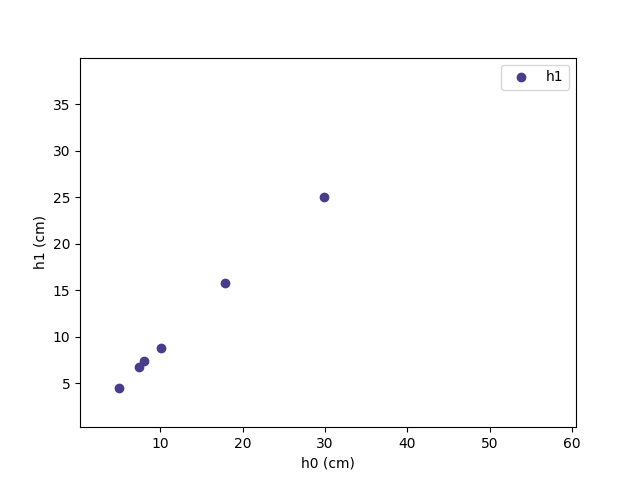
\includegraphics{Metodo1/computed_data/zoom_pallina1.png}
			} %close resize
		} %close centering
		\caption{Figura1: \(h1_{(h0)}\) - pallina da ping pong su parquet}
	\end{figure}
	
	\noindent Interpolazione lineare con il metodo dei minimi quadrati pesati\\
	\[ con\quad\Delta = N(\sum \frac{x_{i}^{2}}{\sigma _{y_{i}}^{2}})-(\sum \frac{x_{i}}{\sigma _{y_{i}}^{2}})^{2}\]\\
	\[B = \frac{N(\sum\frac{x_{i}y_{i}}{\sigma _{y_{i}}^{2}})-\sum\frac{x_{i}}{\sigma _{y_{i}}^{2}}\sum\frac{y_{i}}{\sigma _{y_{i}}^{2}}}{\Delta } \quad
	\sigma _{B} = \sqrt{\frac{\sum \frac{1}{\sigma _{y_{i}}^{2}}}{\Delta}} \qquad
	\Rightarrow \qquad B = 0.814 \pm 0.002\]\\
	\[A = \frac{\sum \frac{(x_{i})^{2}}{\sigma _{y_{i}}^{2}}\sum \frac{(y_{i})^{2}}{\sigma _{y_{i}}^{2}}-\sum \frac{x_{i}}{\sigma _{y_{i}}^{2}}\sum \frac{x_{i}y_{i}}{\sigma _{y_{i}}^{2}}}{\Delta} \quad  \sigma _{A} = \sqrt{\frac{\sum \frac{x^{2}}{\sigma _{y_{i}}^{2}}}{\Delta}} \qquad \Rightarrow \qquad A = 0.75 \pm 0.03\]
	.\\\\\\\\\\\\\\\\
	
	
	\begin{figure}[!ht]
		\captionsetup{labelformat = empty}
		\makebox[1 \textwidth][c]{       %centering table
			\resizebox{0.7 \textwidth}{!}{   %resize table
				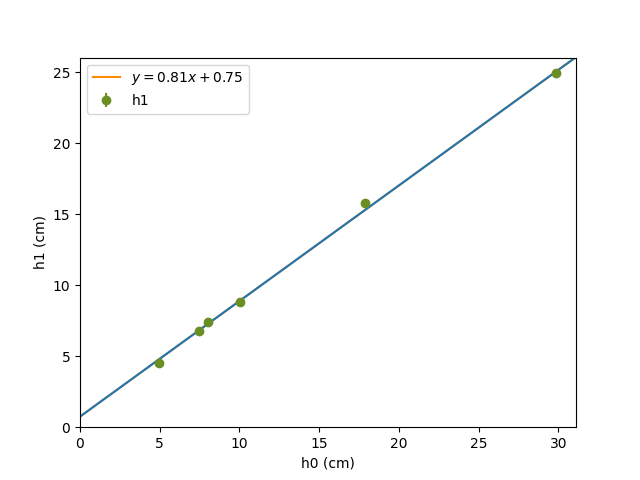
\includegraphics{Metodo1/computed_data/interpolazione_pallina1.png}
			} %close resize
		} %close centering
	\caption{Figura2: \(h1_{(h_{0})}\) - pallina da ping pong - interpolazione}
	\end{figure}
	
\noindent Stima del coefficiente di restituzione e della sua incertezza

	\[ev = \sqrt{\frac{h_{1}}{h_{0}}} \rightarrow ev = \sqrt{B}\]
	
	\makebox[\textwidth]{
		{	
			\small
			dove B = coefficiente angolare della retta \(h_{1}(h_{0})\)
			
		}
	}
\\\\
	\makebox[\textwidth]{
		{	
			\normalsize
	propagazione degli errori \(\rightarrow \quad  \sigma _{ev} = \frac{\sigma _{B}}{2\sqrt{B}} \)
		}
	}
	 \[ev = 0.902 \pm 0.001\]
	 \noindent Test del chi quadro\\
	 \[\chi ^{2} = \sum \left ( \frac{y_{i}-A-BX_{i}}{\sigma_{i}} \right )^{2} = 14\]
	 \noindent considerando 4 gradi di libertà \(\tilde{\chi}^{2} = 3.5 \rightarrow  \)  probabilità pari a 0.7\(\%\) che le misure abbiano seguito la distribuzione lineare assunta.\\
	 Poichè la probabilità è inferiore al 5 \(\%\), supponiamo di aver commesso errori sistematici nella stima di ev.\\\\
	 Il contributo dell'attrito aereo una volta superata una altezza limite è pari a 
	 \[\frac{F_{attrito \quad aereo}}{F_{peso}} = \frac{\rho_{aria} \pi \cdot 0.4 d^{2}}{4m}h_{lim}\]
	 considerando \(h_{lim} = 10 cm\), la massa della pallina come 0.0027Kg ed il diametro d =0.055 metri, tale rapporto equivale a: 0.043.\\
	 \( \rightarrow \) l'effetto dell'accelerazione di gravità sulla pallina, a causa dell'attrito, è ridotto del 4.3\(\%\).\\\\\\\\\\\\
	 Abbiamo corretto l'errore riducendo la regione di interpolazione al di sotto dei 10 cm:
	 \[B = 0.944 \pm 0.015\]
	 \[A = (-0.18 \pm 0.11) cm\] 
	 dai risultati della interpolazione corretta possiamo stimare nuovamente il coeffieciente di restituzione come \(ev = 0.971 \pm 0.008 \)
	 \[\chi ^{2}corretto = 0.697\]
	 nel caso con soli 3 punti possiamo considerare l'ipotesi vera, con una sicurezza del 37 \(\%\). Questa stima corretta del coefficiente di restituzione verrà confrontata con quella ricavata con il metodo 2.
	\subsubsection*{metodo 2}

	
	%metodo due pallina 1
	\noindent Intervalli misurati da 8cm in secondi:

	\begin{figure}[!h]
		\makebox[1 \textwidth][c]{
			\begin{tabular}{c|*{6}{c}}
				numero rimbalzo & lancio1 & lancio2 & lancio3 & lancio4 & lancio5 & media\\
				\hline
				1 & 0.255 & 0.253 & 0.251 & 0.250 & 0.249 & \(0.2516 \pm 0.0010\)\\
				\hline
				2 & 0.242 & 0.239 & 0.238 & 0.237 & 0.236 & \( 0.2384\pm 0.0010\)\\
				\hline
				3 & 0.226 & 0.233 & 0.226 & 0.225 & 0.223 & \( 0.2270\pm 0.0018 \)\\
				\hline
				4 & 0.217 & 0.213 & 0.213 & 0.214 & 0.212 & \( 0.2140\pm 0.0009\)  \\
				\hline
				5 & 0.207 & 0.202 & 0.203 & 0.203 & 0.201 &\( 0.2033\pm 0.0009\) \\
				\hline
				6 & 0.196 & 0.191 & 0.193 & 0.193 & 0.192 & \( 0.1928\pm 0.0008\)\\
				\hline
				7 & 0.183 & 0.182 & 0.183 & 0.183 & 0.182 & \(0.1825\pm 0.00015\)\\
				\hline
				8 & 0.174 & 0.173 & 0.175 & 0.174 & 0.174 &  \(0.1738\pm 0.0003\)\\
				\hline

			\end{tabular}
		} 
	\end{figure}
	\noindent Intervalli misurati da 10cm in secondi:

	\begin{figure}[!h]
		\makebox[1 \textwidth][c]{
			\begin{tabular}{c|*{6}{c}}
				numero rimbalzo & lancio1 & lancio2 & lancio3 & lancio4 & lancio5 &media\\
				\hline
				1 & 0.277 & 0.273 & 0.275 & 0.277 & 0.274 &\(0.2751 \pm 0.0007\) \\
				\hline
				2 & 0.262 & 0.258 & 0.263 & 0.259 & 0.261 & \( 0.2607\pm0.0010\)\\
				\hline
				3 & 0.247 & 0.245 & 0.245 & 0.247 & 0.244 & \(0.2456 \pm 0.0007\)\\
				\hline
				4 & 0.235 & 0.235 & 0.231 & 0.234 & 0.231 & \( 0.2331 \pm 0.0009\)\\
				\hline
				5 & 0.223 & 0.223 & 0.218 & 0.222 & 0.219 & \( 0.2211\pm 0.0011\)\\
				\hline
				6 & 0.205 & 0.211 & 0.205 & 0.211 & 0.207 &\( 0.2078\pm 0.0013\) \\
				\hline
				7 & 0.201 & 0.200 & 0.194 & 0.200 & 0.197 & \(0.1985\pm 0.0012\)\\
				\hline
				8 & 0.190 & 0.190 & 0.185 & 0.190 & 0.187 & \( 0.1885 \pm 0.0010\)\\
				\hline
			\end{tabular}
		} 
	\end{figure}
	.\\\\\\\\\\\\\\\\\\\\\\
	\noindent Intervalli misurati da 15cm in secondi:
	\begin{figure}[!h]
		\makebox[1 \textwidth][c]{
			\begin{tabular}{c|*{6}{c}}
				numero rimbalzo & lancio1 & lancio2 & lancio3 & lancio4 & lancio5 & media\\
				\hline
				1 & 0.339 & 0.341 & 0.339 & 0.340 & 0.337 &\(0.3390 \pm 0.0006\) \\
				\hline
				2 & 0.318 & 0.319 & 0.319 & 0.319 & 0.317 &\( 0.3185 \pm 0.0003\)  \\
				\hline
				3 & 0.298 & 0.299 & 0.299 & 0.299 & 0.297 &  \( 0.2984 \pm 0.0004 \)\\
				\hline
				4 & 0.281 & 0.282 & 0.282 & 0.281 & 0.280 &  \(0.2813\pm 0.0004\)\\
				\hline
				5 & 0.265 & 0.266 & 0.266 & 0.266 & 0.268 & \( 0.2663 \pm0.0005 \)  \\
				\hline
				6 & 0.250 & 0.253 & 0.251 & 0.251 & 0.251 &  \( 0.2511\pm 0.0004\)\\
				\hline
				7 & 0.233 & 0.237 & 0.236 & 0.236 & 0.237 & \(	0.23583\pm 0.0008 \) \\
				\hline
				8 & 0.219 & 0.225 & 0.224 & 0.224 & 0.224 & \( 0.2234\pm 0.0011 \) \\
				\hline
			\end{tabular}
		} 
	\end{figure}

	\noindent Intervalli misurati da 18cm in secondi:
	\begin{figure}[!h]
		\makebox[1 \textwidth][c]{
			\begin{tabular}{c|*{7}{c}}
				numero rimbalzo & lancio1 & lancio2 & lancio3 & lancio4 & lancio5 & media\\
				\hline
				1 & 0.363 & 0.368 & 0.367 & 0.368 & 0.362 & \(0.3656\pm0.0013 \)\\
				\hline
				2 & 0.339 & 0.342 & 0.341 & 0.344 & 0.338 &\( 0.3410\pm 0.0011\)\\
				\hline
				3 & 0.318 & 0.320 & 0.320 & 0.323 & 0.318 &\( 0.3199\pm0.0010\)\\
				\hline
				4 & 0.298 & 0.301 & 0.300 & 0.302 & 0.298 &\(  0.3000\pm0.0009\)\\
				\hline
				5 & 0.282 & 0.283 & 0.282 & 0.285 & 0.281 & \(  0.2829 \pm0.0007 \)\\
				\hline
				6 & 0.261 & 0.265 & 0.269 & 0.269 & 0.264 &\( 0.2657\pm 0.0014\)\\
				\hline
				7 & 0.247 & 0.251 & 0.251 & 0.255 & 0.251 &\(0.2510 \pm 0.0012\)\\
				\hline
				8 & 0.233 & 0.237 & 0.232 & 0.238 & 0.238 & \(  0.2357\pm0.0012\)\\
				\hline
			\end{tabular}
		} 
	\end{figure}

	\noindent Intervalli misurati da 30cm in secondi:
	\begin{figure}[!h]
		\makebox[1 \textwidth][c]{
			\begin{tabular}{c|*{7}{c}}
				numero rimbalzo & lancio1 & lancio2 & lancio3 & lancio4 & lancio5 & media\\
				\hline
				1 & 0.462 & 0.459 & 0.460 & 0.463 & 0.460 & \(0.4608  \pm0.0007 \)\\
				\hline
				2 & 0.425 & 0.424 & 0.425 & 0.422 & 0.424 &\( 0.4231\pm0.0005 \) \\
				\hline
				3 & 0.394 & 0.390 & 0.395 & 0.391 & 0.392 & \( 0.3926 \pm0.0008 \)\\
				\hline
				4 & 0.365 & 0.364 & 0.368 & 0.364 & 0.365 &\(0.3652 \pm0.0008 \) \\
				\hline
				5 & 0.344 & 0.340 & 0.339 & 0.340 & 0.340 & \(0.3407\pm0.0008\)\\
				\hline
				6 & 0.323 & 0.320 & 0.323 & 0.318 & 0.320 & \(  0.3206\pm0.0009 \)\\
				\hline
				7 & 0.299 & 0.299 & 0.304 & 0.298 & 0.298 & \(0.3000\pm 0.0010\)\\
				\hline
				8 & 0.286 & 0.282 & 0.281 & 0.280 & 0.281 & \( 0.2822 \pm 0.0009\)\\
				\hline
			\end{tabular}
		} 
	\end{figure}
.\\\\\\\\\\\\\\\\\\\\\\	
	\noindent Abbiamo sfruttato la relazione \(log(t_{n}) = log(\frac{2v_{0}}{g})+nlog(e_{v})\), che evidenzia la dipendenza lineare del \(log(t_{n})\) rispetto al numero di rimbalzi n.
	\begin{figure}[!ht]
		\captionsetup{labelformat=empty}
		\makebox[1 \textwidth][c]{       %centering table
			\resizebox{0.7 \textwidth}{!}{   %resize table
				%%% Creator: Matplotlib, PGF backend
%%
%% To include the figure in your LaTeX document, write
%%   \input{<filename>.pgf}
%%
%% Make sure the required packages are loaded in your preamble
%%   \usepackage{pgf}
%%
%% and, on pdftex
%%   \usepackage[utf8]{inputenc}\DeclareUnicodeCharacter{2212}{-}
%%
%% or, on luatex and xetex
%%   \usepackage{unicode-math}
%%
%% Figures using additional raster images can only be included by \input if
%% they are in the same directory as the main LaTeX file. For loading figures
%% from other directories you can use the `import` package
%%   \usepackage{import}
%%
%% and then include the figures with
%%   \import{<path to file>}{<filename>.pgf}
%%
%% Matplotlib used the following preamble
%%   \usepackage{fontspec}
%%   \setmainfont{DejaVuSerif.ttf}[Path=C:/Users/giuly/AppData/Local/Programs/Python/Python39/Lib/site-packages/matplotlib/mpl-data/fonts/ttf/]
%%   \setsansfont{DejaVuSans.ttf}[Path=C:/Users/giuly/AppData/Local/Programs/Python/Python39/Lib/site-packages/matplotlib/mpl-data/fonts/ttf/]
%%   \setmonofont{DejaVuSansMono.ttf}[Path=C:/Users/giuly/AppData/Local/Programs/Python/Python39/Lib/site-packages/matplotlib/mpl-data/fonts/ttf/]
%%
\begingroup%
\makeatletter%
\begin{pgfpicture}%
\pgfpathrectangle{\pgfpointorigin}{\pgfqpoint{6.400000in}{4.800000in}}%
\pgfusepath{use as bounding box, clip}%
\begin{pgfscope}%
\pgfsetbuttcap%
\pgfsetmiterjoin%
\definecolor{currentfill}{rgb}{1.000000,1.000000,1.000000}%
\pgfsetfillcolor{currentfill}%
\pgfsetlinewidth{0.000000pt}%
\definecolor{currentstroke}{rgb}{1.000000,1.000000,1.000000}%
\pgfsetstrokecolor{currentstroke}%
\pgfsetdash{}{0pt}%
\pgfpathmoveto{\pgfqpoint{0.000000in}{0.000000in}}%
\pgfpathlineto{\pgfqpoint{6.400000in}{0.000000in}}%
\pgfpathlineto{\pgfqpoint{6.400000in}{4.800000in}}%
\pgfpathlineto{\pgfqpoint{0.000000in}{4.800000in}}%
\pgfpathclose%
\pgfusepath{fill}%
\end{pgfscope}%
\begin{pgfscope}%
\pgfsetbuttcap%
\pgfsetmiterjoin%
\definecolor{currentfill}{rgb}{1.000000,1.000000,1.000000}%
\pgfsetfillcolor{currentfill}%
\pgfsetlinewidth{0.000000pt}%
\definecolor{currentstroke}{rgb}{0.000000,0.000000,0.000000}%
\pgfsetstrokecolor{currentstroke}%
\pgfsetstrokeopacity{0.000000}%
\pgfsetdash{}{0pt}%
\pgfpathmoveto{\pgfqpoint{0.800000in}{0.528000in}}%
\pgfpathlineto{\pgfqpoint{5.760000in}{0.528000in}}%
\pgfpathlineto{\pgfqpoint{5.760000in}{4.224000in}}%
\pgfpathlineto{\pgfqpoint{0.800000in}{4.224000in}}%
\pgfpathclose%
\pgfusepath{fill}%
\end{pgfscope}%
\begin{pgfscope}%
\pgfpathrectangle{\pgfqpoint{0.800000in}{0.528000in}}{\pgfqpoint{4.960000in}{3.696000in}}%
\pgfusepath{clip}%
\pgfsetbuttcap%
\pgfsetmiterjoin%
\definecolor{currentfill}{rgb}{0.400000,0.803922,0.666667}%
\pgfsetfillcolor{currentfill}%
\pgfsetfillopacity{0.800000}%
\pgfsetlinewidth{0.000000pt}%
\definecolor{currentstroke}{rgb}{0.000000,0.000000,0.000000}%
\pgfsetstrokecolor{currentstroke}%
\pgfsetstrokeopacity{0.800000}%
\pgfsetdash{}{0pt}%
\pgfpathmoveto{\pgfqpoint{1.025455in}{0.528000in}}%
\pgfpathlineto{\pgfqpoint{1.401212in}{0.528000in}}%
\pgfpathlineto{\pgfqpoint{1.401212in}{0.848000in}}%
\pgfpathlineto{\pgfqpoint{1.025455in}{0.848000in}}%
\pgfpathclose%
\pgfusepath{fill}%
\end{pgfscope}%
\begin{pgfscope}%
\pgfpathrectangle{\pgfqpoint{0.800000in}{0.528000in}}{\pgfqpoint{4.960000in}{3.696000in}}%
\pgfusepath{clip}%
\pgfsetbuttcap%
\pgfsetmiterjoin%
\definecolor{currentfill}{rgb}{0.400000,0.803922,0.666667}%
\pgfsetfillcolor{currentfill}%
\pgfsetfillopacity{0.800000}%
\pgfsetlinewidth{0.000000pt}%
\definecolor{currentstroke}{rgb}{0.000000,0.000000,0.000000}%
\pgfsetstrokecolor{currentstroke}%
\pgfsetstrokeopacity{0.800000}%
\pgfsetdash{}{0pt}%
\pgfpathmoveto{\pgfqpoint{1.401212in}{0.528000in}}%
\pgfpathlineto{\pgfqpoint{1.776970in}{0.528000in}}%
\pgfpathlineto{\pgfqpoint{1.776970in}{0.848000in}}%
\pgfpathlineto{\pgfqpoint{1.401212in}{0.848000in}}%
\pgfpathclose%
\pgfusepath{fill}%
\end{pgfscope}%
\begin{pgfscope}%
\pgfpathrectangle{\pgfqpoint{0.800000in}{0.528000in}}{\pgfqpoint{4.960000in}{3.696000in}}%
\pgfusepath{clip}%
\pgfsetbuttcap%
\pgfsetmiterjoin%
\definecolor{currentfill}{rgb}{0.400000,0.803922,0.666667}%
\pgfsetfillcolor{currentfill}%
\pgfsetfillopacity{0.800000}%
\pgfsetlinewidth{0.000000pt}%
\definecolor{currentstroke}{rgb}{0.000000,0.000000,0.000000}%
\pgfsetstrokecolor{currentstroke}%
\pgfsetstrokeopacity{0.800000}%
\pgfsetdash{}{0pt}%
\pgfpathmoveto{\pgfqpoint{1.776970in}{0.528000in}}%
\pgfpathlineto{\pgfqpoint{2.152727in}{0.528000in}}%
\pgfpathlineto{\pgfqpoint{2.152727in}{1.168000in}}%
\pgfpathlineto{\pgfqpoint{1.776970in}{1.168000in}}%
\pgfpathclose%
\pgfusepath{fill}%
\end{pgfscope}%
\begin{pgfscope}%
\pgfpathrectangle{\pgfqpoint{0.800000in}{0.528000in}}{\pgfqpoint{4.960000in}{3.696000in}}%
\pgfusepath{clip}%
\pgfsetbuttcap%
\pgfsetmiterjoin%
\definecolor{currentfill}{rgb}{0.400000,0.803922,0.666667}%
\pgfsetfillcolor{currentfill}%
\pgfsetfillopacity{0.800000}%
\pgfsetlinewidth{0.000000pt}%
\definecolor{currentstroke}{rgb}{0.000000,0.000000,0.000000}%
\pgfsetstrokecolor{currentstroke}%
\pgfsetstrokeopacity{0.800000}%
\pgfsetdash{}{0pt}%
\pgfpathmoveto{\pgfqpoint{2.152727in}{0.528000in}}%
\pgfpathlineto{\pgfqpoint{2.528485in}{0.528000in}}%
\pgfpathlineto{\pgfqpoint{2.528485in}{1.968000in}}%
\pgfpathlineto{\pgfqpoint{2.152727in}{1.968000in}}%
\pgfpathclose%
\pgfusepath{fill}%
\end{pgfscope}%
\begin{pgfscope}%
\pgfpathrectangle{\pgfqpoint{0.800000in}{0.528000in}}{\pgfqpoint{4.960000in}{3.696000in}}%
\pgfusepath{clip}%
\pgfsetbuttcap%
\pgfsetmiterjoin%
\definecolor{currentfill}{rgb}{0.400000,0.803922,0.666667}%
\pgfsetfillcolor{currentfill}%
\pgfsetfillopacity{0.800000}%
\pgfsetlinewidth{0.000000pt}%
\definecolor{currentstroke}{rgb}{0.000000,0.000000,0.000000}%
\pgfsetstrokecolor{currentstroke}%
\pgfsetstrokeopacity{0.800000}%
\pgfsetdash{}{0pt}%
\pgfpathmoveto{\pgfqpoint{2.528485in}{0.528000in}}%
\pgfpathlineto{\pgfqpoint{2.904242in}{0.528000in}}%
\pgfpathlineto{\pgfqpoint{2.904242in}{2.448000in}}%
\pgfpathlineto{\pgfqpoint{2.528485in}{2.448000in}}%
\pgfpathclose%
\pgfusepath{fill}%
\end{pgfscope}%
\begin{pgfscope}%
\pgfpathrectangle{\pgfqpoint{0.800000in}{0.528000in}}{\pgfqpoint{4.960000in}{3.696000in}}%
\pgfusepath{clip}%
\pgfsetbuttcap%
\pgfsetmiterjoin%
\definecolor{currentfill}{rgb}{0.400000,0.803922,0.666667}%
\pgfsetfillcolor{currentfill}%
\pgfsetfillopacity{0.800000}%
\pgfsetlinewidth{0.000000pt}%
\definecolor{currentstroke}{rgb}{0.000000,0.000000,0.000000}%
\pgfsetstrokecolor{currentstroke}%
\pgfsetstrokeopacity{0.800000}%
\pgfsetdash{}{0pt}%
\pgfpathmoveto{\pgfqpoint{2.904242in}{0.528000in}}%
\pgfpathlineto{\pgfqpoint{3.280000in}{0.528000in}}%
\pgfpathlineto{\pgfqpoint{3.280000in}{4.048000in}}%
\pgfpathlineto{\pgfqpoint{2.904242in}{4.048000in}}%
\pgfpathclose%
\pgfusepath{fill}%
\end{pgfscope}%
\begin{pgfscope}%
\pgfpathrectangle{\pgfqpoint{0.800000in}{0.528000in}}{\pgfqpoint{4.960000in}{3.696000in}}%
\pgfusepath{clip}%
\pgfsetbuttcap%
\pgfsetmiterjoin%
\definecolor{currentfill}{rgb}{0.400000,0.803922,0.666667}%
\pgfsetfillcolor{currentfill}%
\pgfsetfillopacity{0.800000}%
\pgfsetlinewidth{0.000000pt}%
\definecolor{currentstroke}{rgb}{0.000000,0.000000,0.000000}%
\pgfsetstrokecolor{currentstroke}%
\pgfsetstrokeopacity{0.800000}%
\pgfsetdash{}{0pt}%
\pgfpathmoveto{\pgfqpoint{3.280000in}{0.528000in}}%
\pgfpathlineto{\pgfqpoint{3.655758in}{0.528000in}}%
\pgfpathlineto{\pgfqpoint{3.655758in}{3.248000in}}%
\pgfpathlineto{\pgfqpoint{3.280000in}{3.248000in}}%
\pgfpathclose%
\pgfusepath{fill}%
\end{pgfscope}%
\begin{pgfscope}%
\pgfpathrectangle{\pgfqpoint{0.800000in}{0.528000in}}{\pgfqpoint{4.960000in}{3.696000in}}%
\pgfusepath{clip}%
\pgfsetbuttcap%
\pgfsetmiterjoin%
\definecolor{currentfill}{rgb}{0.400000,0.803922,0.666667}%
\pgfsetfillcolor{currentfill}%
\pgfsetfillopacity{0.800000}%
\pgfsetlinewidth{0.000000pt}%
\definecolor{currentstroke}{rgb}{0.000000,0.000000,0.000000}%
\pgfsetstrokecolor{currentstroke}%
\pgfsetstrokeopacity{0.800000}%
\pgfsetdash{}{0pt}%
\pgfpathmoveto{\pgfqpoint{3.655758in}{0.528000in}}%
\pgfpathlineto{\pgfqpoint{4.031515in}{0.528000in}}%
\pgfpathlineto{\pgfqpoint{4.031515in}{3.248000in}}%
\pgfpathlineto{\pgfqpoint{3.655758in}{3.248000in}}%
\pgfpathclose%
\pgfusepath{fill}%
\end{pgfscope}%
\begin{pgfscope}%
\pgfpathrectangle{\pgfqpoint{0.800000in}{0.528000in}}{\pgfqpoint{4.960000in}{3.696000in}}%
\pgfusepath{clip}%
\pgfsetbuttcap%
\pgfsetmiterjoin%
\definecolor{currentfill}{rgb}{0.400000,0.803922,0.666667}%
\pgfsetfillcolor{currentfill}%
\pgfsetfillopacity{0.800000}%
\pgfsetlinewidth{0.000000pt}%
\definecolor{currentstroke}{rgb}{0.000000,0.000000,0.000000}%
\pgfsetstrokecolor{currentstroke}%
\pgfsetstrokeopacity{0.800000}%
\pgfsetdash{}{0pt}%
\pgfpathmoveto{\pgfqpoint{4.031515in}{0.528000in}}%
\pgfpathlineto{\pgfqpoint{4.407273in}{0.528000in}}%
\pgfpathlineto{\pgfqpoint{4.407273in}{1.968000in}}%
\pgfpathlineto{\pgfqpoint{4.031515in}{1.968000in}}%
\pgfpathclose%
\pgfusepath{fill}%
\end{pgfscope}%
\begin{pgfscope}%
\pgfpathrectangle{\pgfqpoint{0.800000in}{0.528000in}}{\pgfqpoint{4.960000in}{3.696000in}}%
\pgfusepath{clip}%
\pgfsetbuttcap%
\pgfsetmiterjoin%
\definecolor{currentfill}{rgb}{0.400000,0.803922,0.666667}%
\pgfsetfillcolor{currentfill}%
\pgfsetfillopacity{0.800000}%
\pgfsetlinewidth{0.000000pt}%
\definecolor{currentstroke}{rgb}{0.000000,0.000000,0.000000}%
\pgfsetstrokecolor{currentstroke}%
\pgfsetstrokeopacity{0.800000}%
\pgfsetdash{}{0pt}%
\pgfpathmoveto{\pgfqpoint{4.407273in}{0.528000in}}%
\pgfpathlineto{\pgfqpoint{4.783030in}{0.528000in}}%
\pgfpathlineto{\pgfqpoint{4.783030in}{1.168000in}}%
\pgfpathlineto{\pgfqpoint{4.407273in}{1.168000in}}%
\pgfpathclose%
\pgfusepath{fill}%
\end{pgfscope}%
\begin{pgfscope}%
\pgfpathrectangle{\pgfqpoint{0.800000in}{0.528000in}}{\pgfqpoint{4.960000in}{3.696000in}}%
\pgfusepath{clip}%
\pgfsetbuttcap%
\pgfsetmiterjoin%
\definecolor{currentfill}{rgb}{0.400000,0.803922,0.666667}%
\pgfsetfillcolor{currentfill}%
\pgfsetfillopacity{0.800000}%
\pgfsetlinewidth{0.000000pt}%
\definecolor{currentstroke}{rgb}{0.000000,0.000000,0.000000}%
\pgfsetstrokecolor{currentstroke}%
\pgfsetstrokeopacity{0.800000}%
\pgfsetdash{}{0pt}%
\pgfpathmoveto{\pgfqpoint{4.783030in}{0.528000in}}%
\pgfpathlineto{\pgfqpoint{5.158788in}{0.528000in}}%
\pgfpathlineto{\pgfqpoint{5.158788in}{0.688000in}}%
\pgfpathlineto{\pgfqpoint{4.783030in}{0.688000in}}%
\pgfpathclose%
\pgfusepath{fill}%
\end{pgfscope}%
\begin{pgfscope}%
\pgfpathrectangle{\pgfqpoint{0.800000in}{0.528000in}}{\pgfqpoint{4.960000in}{3.696000in}}%
\pgfusepath{clip}%
\pgfsetbuttcap%
\pgfsetmiterjoin%
\definecolor{currentfill}{rgb}{0.400000,0.803922,0.666667}%
\pgfsetfillcolor{currentfill}%
\pgfsetfillopacity{0.800000}%
\pgfsetlinewidth{0.000000pt}%
\definecolor{currentstroke}{rgb}{0.000000,0.000000,0.000000}%
\pgfsetstrokecolor{currentstroke}%
\pgfsetstrokeopacity{0.800000}%
\pgfsetdash{}{0pt}%
\pgfpathmoveto{\pgfqpoint{5.158788in}{0.528000in}}%
\pgfpathlineto{\pgfqpoint{5.534545in}{0.528000in}}%
\pgfpathlineto{\pgfqpoint{5.534545in}{0.688000in}}%
\pgfpathlineto{\pgfqpoint{5.158788in}{0.688000in}}%
\pgfpathclose%
\pgfusepath{fill}%
\end{pgfscope}%
\begin{pgfscope}%
\pgfsetbuttcap%
\pgfsetroundjoin%
\definecolor{currentfill}{rgb}{0.000000,0.000000,0.000000}%
\pgfsetfillcolor{currentfill}%
\pgfsetlinewidth{0.803000pt}%
\definecolor{currentstroke}{rgb}{0.000000,0.000000,0.000000}%
\pgfsetstrokecolor{currentstroke}%
\pgfsetdash{}{0pt}%
\pgfsys@defobject{currentmarker}{\pgfqpoint{0.000000in}{-0.048611in}}{\pgfqpoint{0.000000in}{0.000000in}}{%
\pgfpathmoveto{\pgfqpoint{0.000000in}{0.000000in}}%
\pgfpathlineto{\pgfqpoint{0.000000in}{-0.048611in}}%
\pgfusepath{stroke,fill}%
}%
\begin{pgfscope}%
\pgfsys@transformshift{1.025455in}{0.528000in}%
\pgfsys@useobject{currentmarker}{}%
\end{pgfscope}%
\end{pgfscope}%
\begin{pgfscope}%
\definecolor{textcolor}{rgb}{0.000000,0.000000,0.000000}%
\pgfsetstrokecolor{textcolor}%
\pgfsetfillcolor{textcolor}%
\pgftext[x=1.025455in,y=0.430778in,,top]{\color{textcolor}\sffamily\fontsize{10.000000}{12.000000}\selectfont 1.30}%
\end{pgfscope}%
\begin{pgfscope}%
\pgfsetbuttcap%
\pgfsetroundjoin%
\definecolor{currentfill}{rgb}{0.000000,0.000000,0.000000}%
\pgfsetfillcolor{currentfill}%
\pgfsetlinewidth{0.803000pt}%
\definecolor{currentstroke}{rgb}{0.000000,0.000000,0.000000}%
\pgfsetstrokecolor{currentstroke}%
\pgfsetdash{}{0pt}%
\pgfsys@defobject{currentmarker}{\pgfqpoint{0.000000in}{-0.048611in}}{\pgfqpoint{0.000000in}{0.000000in}}{%
\pgfpathmoveto{\pgfqpoint{0.000000in}{0.000000in}}%
\pgfpathlineto{\pgfqpoint{0.000000in}{-0.048611in}}%
\pgfusepath{stroke,fill}%
}%
\begin{pgfscope}%
\pgfsys@transformshift{1.589091in}{0.528000in}%
\pgfsys@useobject{currentmarker}{}%
\end{pgfscope}%
\end{pgfscope}%
\begin{pgfscope}%
\definecolor{textcolor}{rgb}{0.000000,0.000000,0.000000}%
\pgfsetstrokecolor{textcolor}%
\pgfsetfillcolor{textcolor}%
\pgftext[x=1.589091in,y=0.430778in,,top]{\color{textcolor}\sffamily\fontsize{10.000000}{12.000000}\selectfont 1.35}%
\end{pgfscope}%
\begin{pgfscope}%
\pgfsetbuttcap%
\pgfsetroundjoin%
\definecolor{currentfill}{rgb}{0.000000,0.000000,0.000000}%
\pgfsetfillcolor{currentfill}%
\pgfsetlinewidth{0.803000pt}%
\definecolor{currentstroke}{rgb}{0.000000,0.000000,0.000000}%
\pgfsetstrokecolor{currentstroke}%
\pgfsetdash{}{0pt}%
\pgfsys@defobject{currentmarker}{\pgfqpoint{0.000000in}{-0.048611in}}{\pgfqpoint{0.000000in}{0.000000in}}{%
\pgfpathmoveto{\pgfqpoint{0.000000in}{0.000000in}}%
\pgfpathlineto{\pgfqpoint{0.000000in}{-0.048611in}}%
\pgfusepath{stroke,fill}%
}%
\begin{pgfscope}%
\pgfsys@transformshift{2.152727in}{0.528000in}%
\pgfsys@useobject{currentmarker}{}%
\end{pgfscope}%
\end{pgfscope}%
\begin{pgfscope}%
\definecolor{textcolor}{rgb}{0.000000,0.000000,0.000000}%
\pgfsetstrokecolor{textcolor}%
\pgfsetfillcolor{textcolor}%
\pgftext[x=2.152727in,y=0.430778in,,top]{\color{textcolor}\sffamily\fontsize{10.000000}{12.000000}\selectfont 1.40}%
\end{pgfscope}%
\begin{pgfscope}%
\pgfsetbuttcap%
\pgfsetroundjoin%
\definecolor{currentfill}{rgb}{0.000000,0.000000,0.000000}%
\pgfsetfillcolor{currentfill}%
\pgfsetlinewidth{0.803000pt}%
\definecolor{currentstroke}{rgb}{0.000000,0.000000,0.000000}%
\pgfsetstrokecolor{currentstroke}%
\pgfsetdash{}{0pt}%
\pgfsys@defobject{currentmarker}{\pgfqpoint{0.000000in}{-0.048611in}}{\pgfqpoint{0.000000in}{0.000000in}}{%
\pgfpathmoveto{\pgfqpoint{0.000000in}{0.000000in}}%
\pgfpathlineto{\pgfqpoint{0.000000in}{-0.048611in}}%
\pgfusepath{stroke,fill}%
}%
\begin{pgfscope}%
\pgfsys@transformshift{2.716364in}{0.528000in}%
\pgfsys@useobject{currentmarker}{}%
\end{pgfscope}%
\end{pgfscope}%
\begin{pgfscope}%
\definecolor{textcolor}{rgb}{0.000000,0.000000,0.000000}%
\pgfsetstrokecolor{textcolor}%
\pgfsetfillcolor{textcolor}%
\pgftext[x=2.716364in,y=0.430778in,,top]{\color{textcolor}\sffamily\fontsize{10.000000}{12.000000}\selectfont 1.45}%
\end{pgfscope}%
\begin{pgfscope}%
\pgfsetbuttcap%
\pgfsetroundjoin%
\definecolor{currentfill}{rgb}{0.000000,0.000000,0.000000}%
\pgfsetfillcolor{currentfill}%
\pgfsetlinewidth{0.803000pt}%
\definecolor{currentstroke}{rgb}{0.000000,0.000000,0.000000}%
\pgfsetstrokecolor{currentstroke}%
\pgfsetdash{}{0pt}%
\pgfsys@defobject{currentmarker}{\pgfqpoint{0.000000in}{-0.048611in}}{\pgfqpoint{0.000000in}{0.000000in}}{%
\pgfpathmoveto{\pgfqpoint{0.000000in}{0.000000in}}%
\pgfpathlineto{\pgfqpoint{0.000000in}{-0.048611in}}%
\pgfusepath{stroke,fill}%
}%
\begin{pgfscope}%
\pgfsys@transformshift{3.280000in}{0.528000in}%
\pgfsys@useobject{currentmarker}{}%
\end{pgfscope}%
\end{pgfscope}%
\begin{pgfscope}%
\definecolor{textcolor}{rgb}{0.000000,0.000000,0.000000}%
\pgfsetstrokecolor{textcolor}%
\pgfsetfillcolor{textcolor}%
\pgftext[x=3.280000in,y=0.430778in,,top]{\color{textcolor}\sffamily\fontsize{10.000000}{12.000000}\selectfont 1.50}%
\end{pgfscope}%
\begin{pgfscope}%
\pgfsetbuttcap%
\pgfsetroundjoin%
\definecolor{currentfill}{rgb}{0.000000,0.000000,0.000000}%
\pgfsetfillcolor{currentfill}%
\pgfsetlinewidth{0.803000pt}%
\definecolor{currentstroke}{rgb}{0.000000,0.000000,0.000000}%
\pgfsetstrokecolor{currentstroke}%
\pgfsetdash{}{0pt}%
\pgfsys@defobject{currentmarker}{\pgfqpoint{0.000000in}{-0.048611in}}{\pgfqpoint{0.000000in}{0.000000in}}{%
\pgfpathmoveto{\pgfqpoint{0.000000in}{0.000000in}}%
\pgfpathlineto{\pgfqpoint{0.000000in}{-0.048611in}}%
\pgfusepath{stroke,fill}%
}%
\begin{pgfscope}%
\pgfsys@transformshift{3.843636in}{0.528000in}%
\pgfsys@useobject{currentmarker}{}%
\end{pgfscope}%
\end{pgfscope}%
\begin{pgfscope}%
\definecolor{textcolor}{rgb}{0.000000,0.000000,0.000000}%
\pgfsetstrokecolor{textcolor}%
\pgfsetfillcolor{textcolor}%
\pgftext[x=3.843636in,y=0.430778in,,top]{\color{textcolor}\sffamily\fontsize{10.000000}{12.000000}\selectfont 1.55}%
\end{pgfscope}%
\begin{pgfscope}%
\pgfsetbuttcap%
\pgfsetroundjoin%
\definecolor{currentfill}{rgb}{0.000000,0.000000,0.000000}%
\pgfsetfillcolor{currentfill}%
\pgfsetlinewidth{0.803000pt}%
\definecolor{currentstroke}{rgb}{0.000000,0.000000,0.000000}%
\pgfsetstrokecolor{currentstroke}%
\pgfsetdash{}{0pt}%
\pgfsys@defobject{currentmarker}{\pgfqpoint{0.000000in}{-0.048611in}}{\pgfqpoint{0.000000in}{0.000000in}}{%
\pgfpathmoveto{\pgfqpoint{0.000000in}{0.000000in}}%
\pgfpathlineto{\pgfqpoint{0.000000in}{-0.048611in}}%
\pgfusepath{stroke,fill}%
}%
\begin{pgfscope}%
\pgfsys@transformshift{4.407273in}{0.528000in}%
\pgfsys@useobject{currentmarker}{}%
\end{pgfscope}%
\end{pgfscope}%
\begin{pgfscope}%
\definecolor{textcolor}{rgb}{0.000000,0.000000,0.000000}%
\pgfsetstrokecolor{textcolor}%
\pgfsetfillcolor{textcolor}%
\pgftext[x=4.407273in,y=0.430778in,,top]{\color{textcolor}\sffamily\fontsize{10.000000}{12.000000}\selectfont 1.60}%
\end{pgfscope}%
\begin{pgfscope}%
\pgfsetbuttcap%
\pgfsetroundjoin%
\definecolor{currentfill}{rgb}{0.000000,0.000000,0.000000}%
\pgfsetfillcolor{currentfill}%
\pgfsetlinewidth{0.803000pt}%
\definecolor{currentstroke}{rgb}{0.000000,0.000000,0.000000}%
\pgfsetstrokecolor{currentstroke}%
\pgfsetdash{}{0pt}%
\pgfsys@defobject{currentmarker}{\pgfqpoint{0.000000in}{-0.048611in}}{\pgfqpoint{0.000000in}{0.000000in}}{%
\pgfpathmoveto{\pgfqpoint{0.000000in}{0.000000in}}%
\pgfpathlineto{\pgfqpoint{0.000000in}{-0.048611in}}%
\pgfusepath{stroke,fill}%
}%
\begin{pgfscope}%
\pgfsys@transformshift{4.970909in}{0.528000in}%
\pgfsys@useobject{currentmarker}{}%
\end{pgfscope}%
\end{pgfscope}%
\begin{pgfscope}%
\definecolor{textcolor}{rgb}{0.000000,0.000000,0.000000}%
\pgfsetstrokecolor{textcolor}%
\pgfsetfillcolor{textcolor}%
\pgftext[x=4.970909in,y=0.430778in,,top]{\color{textcolor}\sffamily\fontsize{10.000000}{12.000000}\selectfont 1.65}%
\end{pgfscope}%
\begin{pgfscope}%
\pgfsetbuttcap%
\pgfsetroundjoin%
\definecolor{currentfill}{rgb}{0.000000,0.000000,0.000000}%
\pgfsetfillcolor{currentfill}%
\pgfsetlinewidth{0.803000pt}%
\definecolor{currentstroke}{rgb}{0.000000,0.000000,0.000000}%
\pgfsetstrokecolor{currentstroke}%
\pgfsetdash{}{0pt}%
\pgfsys@defobject{currentmarker}{\pgfqpoint{0.000000in}{-0.048611in}}{\pgfqpoint{0.000000in}{0.000000in}}{%
\pgfpathmoveto{\pgfqpoint{0.000000in}{0.000000in}}%
\pgfpathlineto{\pgfqpoint{0.000000in}{-0.048611in}}%
\pgfusepath{stroke,fill}%
}%
\begin{pgfscope}%
\pgfsys@transformshift{5.534545in}{0.528000in}%
\pgfsys@useobject{currentmarker}{}%
\end{pgfscope}%
\end{pgfscope}%
\begin{pgfscope}%
\definecolor{textcolor}{rgb}{0.000000,0.000000,0.000000}%
\pgfsetstrokecolor{textcolor}%
\pgfsetfillcolor{textcolor}%
\pgftext[x=5.534545in,y=0.430778in,,top]{\color{textcolor}\sffamily\fontsize{10.000000}{12.000000}\selectfont 1.70}%
\end{pgfscope}%
\begin{pgfscope}%
\definecolor{textcolor}{rgb}{0.000000,0.000000,0.000000}%
\pgfsetstrokecolor{textcolor}%
\pgfsetfillcolor{textcolor}%
\pgftext[x=3.280000in,y=0.240809in,,top]{\color{textcolor}\sffamily\fontsize{10.000000}{12.000000}\selectfont \(\displaystyle x_k\) (s)}%
\end{pgfscope}%
\begin{pgfscope}%
\pgfsetbuttcap%
\pgfsetroundjoin%
\definecolor{currentfill}{rgb}{0.000000,0.000000,0.000000}%
\pgfsetfillcolor{currentfill}%
\pgfsetlinewidth{0.803000pt}%
\definecolor{currentstroke}{rgb}{0.000000,0.000000,0.000000}%
\pgfsetstrokecolor{currentstroke}%
\pgfsetdash{}{0pt}%
\pgfsys@defobject{currentmarker}{\pgfqpoint{-0.048611in}{0.000000in}}{\pgfqpoint{-0.000000in}{0.000000in}}{%
\pgfpathmoveto{\pgfqpoint{-0.000000in}{0.000000in}}%
\pgfpathlineto{\pgfqpoint{-0.048611in}{0.000000in}}%
\pgfusepath{stroke,fill}%
}%
\begin{pgfscope}%
\pgfsys@transformshift{0.800000in}{0.528000in}%
\pgfsys@useobject{currentmarker}{}%
\end{pgfscope}%
\end{pgfscope}%
\begin{pgfscope}%
\definecolor{textcolor}{rgb}{0.000000,0.000000,0.000000}%
\pgfsetstrokecolor{textcolor}%
\pgfsetfillcolor{textcolor}%
\pgftext[x=0.614412in, y=0.475238in, left, base]{\color{textcolor}\sffamily\fontsize{10.000000}{12.000000}\selectfont 0}%
\end{pgfscope}%
\begin{pgfscope}%
\pgfsetbuttcap%
\pgfsetroundjoin%
\definecolor{currentfill}{rgb}{0.000000,0.000000,0.000000}%
\pgfsetfillcolor{currentfill}%
\pgfsetlinewidth{0.803000pt}%
\definecolor{currentstroke}{rgb}{0.000000,0.000000,0.000000}%
\pgfsetstrokecolor{currentstroke}%
\pgfsetdash{}{0pt}%
\pgfsys@defobject{currentmarker}{\pgfqpoint{-0.048611in}{0.000000in}}{\pgfqpoint{-0.000000in}{0.000000in}}{%
\pgfpathmoveto{\pgfqpoint{-0.000000in}{0.000000in}}%
\pgfpathlineto{\pgfqpoint{-0.048611in}{0.000000in}}%
\pgfusepath{stroke,fill}%
}%
\begin{pgfscope}%
\pgfsys@transformshift{0.800000in}{1.061333in}%
\pgfsys@useobject{currentmarker}{}%
\end{pgfscope}%
\end{pgfscope}%
\begin{pgfscope}%
\definecolor{textcolor}{rgb}{0.000000,0.000000,0.000000}%
\pgfsetstrokecolor{textcolor}%
\pgfsetfillcolor{textcolor}%
\pgftext[x=0.614412in, y=1.008572in, left, base]{\color{textcolor}\sffamily\fontsize{10.000000}{12.000000}\selectfont 1}%
\end{pgfscope}%
\begin{pgfscope}%
\pgfsetbuttcap%
\pgfsetroundjoin%
\definecolor{currentfill}{rgb}{0.000000,0.000000,0.000000}%
\pgfsetfillcolor{currentfill}%
\pgfsetlinewidth{0.803000pt}%
\definecolor{currentstroke}{rgb}{0.000000,0.000000,0.000000}%
\pgfsetstrokecolor{currentstroke}%
\pgfsetdash{}{0pt}%
\pgfsys@defobject{currentmarker}{\pgfqpoint{-0.048611in}{0.000000in}}{\pgfqpoint{-0.000000in}{0.000000in}}{%
\pgfpathmoveto{\pgfqpoint{-0.000000in}{0.000000in}}%
\pgfpathlineto{\pgfqpoint{-0.048611in}{0.000000in}}%
\pgfusepath{stroke,fill}%
}%
\begin{pgfscope}%
\pgfsys@transformshift{0.800000in}{1.594667in}%
\pgfsys@useobject{currentmarker}{}%
\end{pgfscope}%
\end{pgfscope}%
\begin{pgfscope}%
\definecolor{textcolor}{rgb}{0.000000,0.000000,0.000000}%
\pgfsetstrokecolor{textcolor}%
\pgfsetfillcolor{textcolor}%
\pgftext[x=0.614412in, y=1.541905in, left, base]{\color{textcolor}\sffamily\fontsize{10.000000}{12.000000}\selectfont 2}%
\end{pgfscope}%
\begin{pgfscope}%
\pgfsetbuttcap%
\pgfsetroundjoin%
\definecolor{currentfill}{rgb}{0.000000,0.000000,0.000000}%
\pgfsetfillcolor{currentfill}%
\pgfsetlinewidth{0.803000pt}%
\definecolor{currentstroke}{rgb}{0.000000,0.000000,0.000000}%
\pgfsetstrokecolor{currentstroke}%
\pgfsetdash{}{0pt}%
\pgfsys@defobject{currentmarker}{\pgfqpoint{-0.048611in}{0.000000in}}{\pgfqpoint{-0.000000in}{0.000000in}}{%
\pgfpathmoveto{\pgfqpoint{-0.000000in}{0.000000in}}%
\pgfpathlineto{\pgfqpoint{-0.048611in}{0.000000in}}%
\pgfusepath{stroke,fill}%
}%
\begin{pgfscope}%
\pgfsys@transformshift{0.800000in}{2.128000in}%
\pgfsys@useobject{currentmarker}{}%
\end{pgfscope}%
\end{pgfscope}%
\begin{pgfscope}%
\definecolor{textcolor}{rgb}{0.000000,0.000000,0.000000}%
\pgfsetstrokecolor{textcolor}%
\pgfsetfillcolor{textcolor}%
\pgftext[x=0.614412in, y=2.075238in, left, base]{\color{textcolor}\sffamily\fontsize{10.000000}{12.000000}\selectfont 3}%
\end{pgfscope}%
\begin{pgfscope}%
\pgfsetbuttcap%
\pgfsetroundjoin%
\definecolor{currentfill}{rgb}{0.000000,0.000000,0.000000}%
\pgfsetfillcolor{currentfill}%
\pgfsetlinewidth{0.803000pt}%
\definecolor{currentstroke}{rgb}{0.000000,0.000000,0.000000}%
\pgfsetstrokecolor{currentstroke}%
\pgfsetdash{}{0pt}%
\pgfsys@defobject{currentmarker}{\pgfqpoint{-0.048611in}{0.000000in}}{\pgfqpoint{-0.000000in}{0.000000in}}{%
\pgfpathmoveto{\pgfqpoint{-0.000000in}{0.000000in}}%
\pgfpathlineto{\pgfqpoint{-0.048611in}{0.000000in}}%
\pgfusepath{stroke,fill}%
}%
\begin{pgfscope}%
\pgfsys@transformshift{0.800000in}{2.661333in}%
\pgfsys@useobject{currentmarker}{}%
\end{pgfscope}%
\end{pgfscope}%
\begin{pgfscope}%
\definecolor{textcolor}{rgb}{0.000000,0.000000,0.000000}%
\pgfsetstrokecolor{textcolor}%
\pgfsetfillcolor{textcolor}%
\pgftext[x=0.614412in, y=2.608572in, left, base]{\color{textcolor}\sffamily\fontsize{10.000000}{12.000000}\selectfont 4}%
\end{pgfscope}%
\begin{pgfscope}%
\pgfsetbuttcap%
\pgfsetroundjoin%
\definecolor{currentfill}{rgb}{0.000000,0.000000,0.000000}%
\pgfsetfillcolor{currentfill}%
\pgfsetlinewidth{0.803000pt}%
\definecolor{currentstroke}{rgb}{0.000000,0.000000,0.000000}%
\pgfsetstrokecolor{currentstroke}%
\pgfsetdash{}{0pt}%
\pgfsys@defobject{currentmarker}{\pgfqpoint{-0.048611in}{0.000000in}}{\pgfqpoint{-0.000000in}{0.000000in}}{%
\pgfpathmoveto{\pgfqpoint{-0.000000in}{0.000000in}}%
\pgfpathlineto{\pgfqpoint{-0.048611in}{0.000000in}}%
\pgfusepath{stroke,fill}%
}%
\begin{pgfscope}%
\pgfsys@transformshift{0.800000in}{3.194667in}%
\pgfsys@useobject{currentmarker}{}%
\end{pgfscope}%
\end{pgfscope}%
\begin{pgfscope}%
\definecolor{textcolor}{rgb}{0.000000,0.000000,0.000000}%
\pgfsetstrokecolor{textcolor}%
\pgfsetfillcolor{textcolor}%
\pgftext[x=0.614412in, y=3.141905in, left, base]{\color{textcolor}\sffamily\fontsize{10.000000}{12.000000}\selectfont 5}%
\end{pgfscope}%
\begin{pgfscope}%
\pgfsetbuttcap%
\pgfsetroundjoin%
\definecolor{currentfill}{rgb}{0.000000,0.000000,0.000000}%
\pgfsetfillcolor{currentfill}%
\pgfsetlinewidth{0.803000pt}%
\definecolor{currentstroke}{rgb}{0.000000,0.000000,0.000000}%
\pgfsetstrokecolor{currentstroke}%
\pgfsetdash{}{0pt}%
\pgfsys@defobject{currentmarker}{\pgfqpoint{-0.048611in}{0.000000in}}{\pgfqpoint{-0.000000in}{0.000000in}}{%
\pgfpathmoveto{\pgfqpoint{-0.000000in}{0.000000in}}%
\pgfpathlineto{\pgfqpoint{-0.048611in}{0.000000in}}%
\pgfusepath{stroke,fill}%
}%
\begin{pgfscope}%
\pgfsys@transformshift{0.800000in}{3.728000in}%
\pgfsys@useobject{currentmarker}{}%
\end{pgfscope}%
\end{pgfscope}%
\begin{pgfscope}%
\definecolor{textcolor}{rgb}{0.000000,0.000000,0.000000}%
\pgfsetstrokecolor{textcolor}%
\pgfsetfillcolor{textcolor}%
\pgftext[x=0.614412in, y=3.675238in, left, base]{\color{textcolor}\sffamily\fontsize{10.000000}{12.000000}\selectfont 6}%
\end{pgfscope}%
\begin{pgfscope}%
\definecolor{textcolor}{rgb}{0.000000,0.000000,0.000000}%
\pgfsetstrokecolor{textcolor}%
\pgfsetfillcolor{textcolor}%
\pgftext[x=0.558857in,y=2.376000in,,bottom,rotate=90.000000]{\color{textcolor}\sffamily\fontsize{10.000000}{12.000000}\selectfont Densità di Frequenza}%
\end{pgfscope}%
\begin{pgfscope}%
\pgfpathrectangle{\pgfqpoint{0.800000in}{0.528000in}}{\pgfqpoint{4.960000in}{3.696000in}}%
\pgfusepath{clip}%
\pgfsetrectcap%
\pgfsetroundjoin%
\pgfsetlinewidth{1.505625pt}%
\definecolor{currentstroke}{rgb}{1.000000,0.549020,0.000000}%
\pgfsetstrokecolor{currentstroke}%
\pgfsetdash{}{0pt}%
\pgfpathmoveto{\pgfqpoint{1.025455in}{0.574044in}}%
\pgfpathlineto{\pgfqpoint{1.117477in}{0.593003in}}%
\pgfpathlineto{\pgfqpoint{1.209499in}{0.618431in}}%
\pgfpathlineto{\pgfqpoint{1.301521in}{0.651974in}}%
\pgfpathlineto{\pgfqpoint{1.393544in}{0.695485in}}%
\pgfpathlineto{\pgfqpoint{1.485566in}{0.750973in}}%
\pgfpathlineto{\pgfqpoint{1.577588in}{0.820521in}}%
\pgfpathlineto{\pgfqpoint{1.669610in}{0.906175in}}%
\pgfpathlineto{\pgfqpoint{1.761633in}{1.009791in}}%
\pgfpathlineto{\pgfqpoint{1.853655in}{1.132860in}}%
\pgfpathlineto{\pgfqpoint{1.945677in}{1.276309in}}%
\pgfpathlineto{\pgfqpoint{2.037699in}{1.440300in}}%
\pgfpathlineto{\pgfqpoint{2.129722in}{1.624034in}}%
\pgfpathlineto{\pgfqpoint{2.221744in}{1.825600in}}%
\pgfpathlineto{\pgfqpoint{2.313766in}{2.041867in}}%
\pgfpathlineto{\pgfqpoint{2.405788in}{2.268464in}}%
\pgfpathlineto{\pgfqpoint{2.497811in}{2.499842in}}%
\pgfpathlineto{\pgfqpoint{2.589833in}{2.729454in}}%
\pgfpathlineto{\pgfqpoint{2.681855in}{2.950017in}}%
\pgfpathlineto{\pgfqpoint{2.773878in}{3.153881in}}%
\pgfpathlineto{\pgfqpoint{2.865900in}{3.333452in}}%
\pgfpathlineto{\pgfqpoint{2.957922in}{3.481663in}}%
\pgfpathlineto{\pgfqpoint{3.049944in}{3.592427in}}%
\pgfpathlineto{\pgfqpoint{3.141967in}{3.661053in}}%
\pgfpathlineto{\pgfqpoint{3.233989in}{3.684577in}}%
\pgfpathlineto{\pgfqpoint{3.326011in}{3.661972in}}%
\pgfpathlineto{\pgfqpoint{3.418033in}{3.594225in}}%
\pgfpathlineto{\pgfqpoint{3.510056in}{3.484264in}}%
\pgfpathlineto{\pgfqpoint{3.602078in}{3.336746in}}%
\pgfpathlineto{\pgfqpoint{3.694100in}{3.157735in}}%
\pgfpathlineto{\pgfqpoint{3.786122in}{2.954284in}}%
\pgfpathlineto{\pgfqpoint{3.878145in}{2.733979in}}%
\pgfpathlineto{\pgfqpoint{3.970167in}{2.504475in}}%
\pgfpathlineto{\pgfqpoint{4.062189in}{2.273065in}}%
\pgfpathlineto{\pgfqpoint{4.154212in}{2.046315in}}%
\pgfpathlineto{\pgfqpoint{4.246234in}{1.829794in}}%
\pgfpathlineto{\pgfqpoint{4.338256in}{1.627899in}}%
\pgfpathlineto{\pgfqpoint{4.430278in}{1.443785in}}%
\pgfpathlineto{\pgfqpoint{4.522301in}{1.279389in}}%
\pgfpathlineto{\pgfqpoint{4.614323in}{1.135527in}}%
\pgfpathlineto{\pgfqpoint{4.706345in}{1.012058in}}%
\pgfpathlineto{\pgfqpoint{4.798367in}{0.908066in}}%
\pgfpathlineto{\pgfqpoint{4.890390in}{0.822070in}}%
\pgfpathlineto{\pgfqpoint{4.982412in}{0.752219in}}%
\pgfpathlineto{\pgfqpoint{5.074434in}{0.696471in}}%
\pgfpathlineto{\pgfqpoint{5.166456in}{0.652740in}}%
\pgfpathlineto{\pgfqpoint{5.258479in}{0.619016in}}%
\pgfpathlineto{\pgfqpoint{5.350501in}{0.593443in}}%
\pgfpathlineto{\pgfqpoint{5.442523in}{0.574370in}}%
\pgfpathlineto{\pgfqpoint{5.534545in}{0.560377in}}%
\pgfusepath{stroke}%
\end{pgfscope}%
\begin{pgfscope}%
\pgfsetrectcap%
\pgfsetmiterjoin%
\pgfsetlinewidth{0.803000pt}%
\definecolor{currentstroke}{rgb}{0.000000,0.000000,0.000000}%
\pgfsetstrokecolor{currentstroke}%
\pgfsetdash{}{0pt}%
\pgfpathmoveto{\pgfqpoint{0.800000in}{0.528000in}}%
\pgfpathlineto{\pgfqpoint{0.800000in}{4.224000in}}%
\pgfusepath{stroke}%
\end{pgfscope}%
\begin{pgfscope}%
\pgfsetrectcap%
\pgfsetmiterjoin%
\pgfsetlinewidth{0.803000pt}%
\definecolor{currentstroke}{rgb}{0.000000,0.000000,0.000000}%
\pgfsetstrokecolor{currentstroke}%
\pgfsetdash{}{0pt}%
\pgfpathmoveto{\pgfqpoint{5.760000in}{0.528000in}}%
\pgfpathlineto{\pgfqpoint{5.760000in}{4.224000in}}%
\pgfusepath{stroke}%
\end{pgfscope}%
\begin{pgfscope}%
\pgfsetrectcap%
\pgfsetmiterjoin%
\pgfsetlinewidth{0.803000pt}%
\definecolor{currentstroke}{rgb}{0.000000,0.000000,0.000000}%
\pgfsetstrokecolor{currentstroke}%
\pgfsetdash{}{0pt}%
\pgfpathmoveto{\pgfqpoint{0.800000in}{0.528000in}}%
\pgfpathlineto{\pgfqpoint{5.760000in}{0.528000in}}%
\pgfusepath{stroke}%
\end{pgfscope}%
\begin{pgfscope}%
\pgfsetrectcap%
\pgfsetmiterjoin%
\pgfsetlinewidth{0.803000pt}%
\definecolor{currentstroke}{rgb}{0.000000,0.000000,0.000000}%
\pgfsetstrokecolor{currentstroke}%
\pgfsetdash{}{0pt}%
\pgfpathmoveto{\pgfqpoint{0.800000in}{4.224000in}}%
\pgfpathlineto{\pgfqpoint{5.760000in}{4.224000in}}%
\pgfusepath{stroke}%
\end{pgfscope}%
\begin{pgfscope}%
\pgfsetbuttcap%
\pgfsetmiterjoin%
\definecolor{currentfill}{rgb}{1.000000,1.000000,1.000000}%
\pgfsetfillcolor{currentfill}%
\pgfsetfillopacity{0.800000}%
\pgfsetlinewidth{1.003750pt}%
\definecolor{currentstroke}{rgb}{0.800000,0.800000,0.800000}%
\pgfsetstrokecolor{currentstroke}%
\pgfsetstrokeopacity{0.800000}%
\pgfsetdash{}{0pt}%
\pgfpathmoveto{\pgfqpoint{4.613473in}{3.690899in}}%
\pgfpathlineto{\pgfqpoint{5.662778in}{3.690899in}}%
\pgfpathquadraticcurveto{\pgfqpoint{5.690556in}{3.690899in}}{\pgfqpoint{5.690556in}{3.718677in}}%
\pgfpathlineto{\pgfqpoint{5.690556in}{4.126778in}}%
\pgfpathquadraticcurveto{\pgfqpoint{5.690556in}{4.154556in}}{\pgfqpoint{5.662778in}{4.154556in}}%
\pgfpathlineto{\pgfqpoint{4.613473in}{4.154556in}}%
\pgfpathquadraticcurveto{\pgfqpoint{4.585695in}{4.154556in}}{\pgfqpoint{4.585695in}{4.126778in}}%
\pgfpathlineto{\pgfqpoint{4.585695in}{3.718677in}}%
\pgfpathquadraticcurveto{\pgfqpoint{4.585695in}{3.690899in}}{\pgfqpoint{4.613473in}{3.690899in}}%
\pgfpathclose%
\pgfusepath{stroke,fill}%
\end{pgfscope}%
\begin{pgfscope}%
\pgfsetrectcap%
\pgfsetroundjoin%
\pgfsetlinewidth{1.505625pt}%
\definecolor{currentstroke}{rgb}{1.000000,0.549020,0.000000}%
\pgfsetstrokecolor{currentstroke}%
\pgfsetdash{}{0pt}%
\pgfpathmoveto{\pgfqpoint{4.641251in}{4.033645in}}%
\pgfpathlineto{\pgfqpoint{4.919029in}{4.033645in}}%
\pgfusepath{stroke}%
\end{pgfscope}%
\begin{pgfscope}%
\definecolor{textcolor}{rgb}{0.000000,0.000000,0.000000}%
\pgfsetstrokecolor{textcolor}%
\pgfsetfillcolor{textcolor}%
\pgftext[x=5.030140in,y=3.985034in,left,base]{\color{textcolor}\sffamily\fontsize{10.000000}{12.000000}\selectfont \(\displaystyle G(x;\bar{T},\sigma)\)}%
\end{pgfscope}%
\begin{pgfscope}%
\pgfsetbuttcap%
\pgfsetmiterjoin%
\definecolor{currentfill}{rgb}{0.400000,0.803922,0.666667}%
\pgfsetfillcolor{currentfill}%
\pgfsetfillopacity{0.800000}%
\pgfsetlinewidth{0.000000pt}%
\definecolor{currentstroke}{rgb}{0.000000,0.000000,0.000000}%
\pgfsetstrokecolor{currentstroke}%
\pgfsetstrokeopacity{0.800000}%
\pgfsetdash{}{0pt}%
\pgfpathmoveto{\pgfqpoint{4.641251in}{3.775344in}}%
\pgfpathlineto{\pgfqpoint{4.919029in}{3.775344in}}%
\pgfpathlineto{\pgfqpoint{4.919029in}{3.872567in}}%
\pgfpathlineto{\pgfqpoint{4.641251in}{3.872567in}}%
\pgfpathclose%
\pgfusepath{fill}%
\end{pgfscope}%
\begin{pgfscope}%
\definecolor{textcolor}{rgb}{0.000000,0.000000,0.000000}%
\pgfsetstrokecolor{textcolor}%
\pgfsetfillcolor{textcolor}%
\pgftext[x=5.030140in,y=3.775344in,left,base]{\color{textcolor}\sffamily\fontsize{10.000000}{12.000000}\selectfont data}%
\end{pgfscope}%
\end{pgfpicture}%
\makeatother%
\endgroup%

				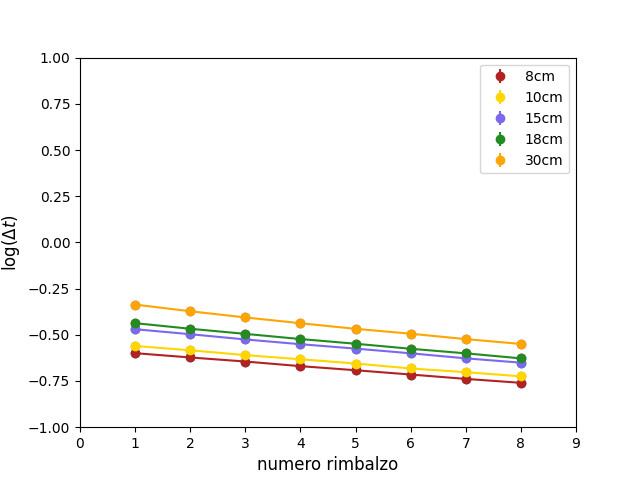
\includegraphics{Metodo2/computed_data/graficoLog_pallina1.png}
			} %close resize
		} %close centering
		\caption{Figura3: \(log\Delta t _{(n)}\) - pallina da ping pong su parquet}
	\end{figure}
	
	\noindent Abbiamo ricavato il coefficiente angolare di ciascuna delle 5 rette tramite il metodo dei minimi quadrati.
	
	\begin{figure}[!ht]
		\captionsetup{labelformat=empty}
		\makebox[1 \textwidth][c]{       %centering table
			\resizebox{0.7 \textwidth}{!}{   %resize table
				%%% Creator: Matplotlib, PGF backend
%%
%% To include the figure in your LaTeX document, write
%%   \input{<filename>.pgf}
%%
%% Make sure the required packages are loaded in your preamble
%%   \usepackage{pgf}
%%
%% and, on pdftex
%%   \usepackage[utf8]{inputenc}\DeclareUnicodeCharacter{2212}{-}
%%
%% or, on luatex and xetex
%%   \usepackage{unicode-math}
%%
%% Figures using additional raster images can only be included by \input if
%% they are in the same directory as the main LaTeX file. For loading figures
%% from other directories you can use the `import` package
%%   \usepackage{import}
%%
%% and then include the figures with
%%   \import{<path to file>}{<filename>.pgf}
%%
%% Matplotlib used the following preamble
%%   \usepackage{fontspec}
%%   \setmainfont{DejaVuSerif.ttf}[Path=C:/Users/giuly/AppData/Local/Programs/Python/Python39/Lib/site-packages/matplotlib/mpl-data/fonts/ttf/]
%%   \setsansfont{DejaVuSans.ttf}[Path=C:/Users/giuly/AppData/Local/Programs/Python/Python39/Lib/site-packages/matplotlib/mpl-data/fonts/ttf/]
%%   \setmonofont{DejaVuSansMono.ttf}[Path=C:/Users/giuly/AppData/Local/Programs/Python/Python39/Lib/site-packages/matplotlib/mpl-data/fonts/ttf/]
%%
\begingroup%
\makeatletter%
\begin{pgfpicture}%
\pgfpathrectangle{\pgfpointorigin}{\pgfqpoint{6.400000in}{4.800000in}}%
\pgfusepath{use as bounding box, clip}%
\begin{pgfscope}%
\pgfsetbuttcap%
\pgfsetmiterjoin%
\definecolor{currentfill}{rgb}{1.000000,1.000000,1.000000}%
\pgfsetfillcolor{currentfill}%
\pgfsetlinewidth{0.000000pt}%
\definecolor{currentstroke}{rgb}{1.000000,1.000000,1.000000}%
\pgfsetstrokecolor{currentstroke}%
\pgfsetdash{}{0pt}%
\pgfpathmoveto{\pgfqpoint{0.000000in}{0.000000in}}%
\pgfpathlineto{\pgfqpoint{6.400000in}{0.000000in}}%
\pgfpathlineto{\pgfqpoint{6.400000in}{4.800000in}}%
\pgfpathlineto{\pgfqpoint{0.000000in}{4.800000in}}%
\pgfpathclose%
\pgfusepath{fill}%
\end{pgfscope}%
\begin{pgfscope}%
\pgfsetbuttcap%
\pgfsetmiterjoin%
\definecolor{currentfill}{rgb}{1.000000,1.000000,1.000000}%
\pgfsetfillcolor{currentfill}%
\pgfsetlinewidth{0.000000pt}%
\definecolor{currentstroke}{rgb}{0.000000,0.000000,0.000000}%
\pgfsetstrokecolor{currentstroke}%
\pgfsetstrokeopacity{0.000000}%
\pgfsetdash{}{0pt}%
\pgfpathmoveto{\pgfqpoint{0.800000in}{0.528000in}}%
\pgfpathlineto{\pgfqpoint{5.760000in}{0.528000in}}%
\pgfpathlineto{\pgfqpoint{5.760000in}{4.224000in}}%
\pgfpathlineto{\pgfqpoint{0.800000in}{4.224000in}}%
\pgfpathclose%
\pgfusepath{fill}%
\end{pgfscope}%
\begin{pgfscope}%
\pgfpathrectangle{\pgfqpoint{0.800000in}{0.528000in}}{\pgfqpoint{4.960000in}{3.696000in}}%
\pgfusepath{clip}%
\pgfsetbuttcap%
\pgfsetmiterjoin%
\definecolor{currentfill}{rgb}{0.400000,0.803922,0.666667}%
\pgfsetfillcolor{currentfill}%
\pgfsetfillopacity{0.800000}%
\pgfsetlinewidth{0.000000pt}%
\definecolor{currentstroke}{rgb}{0.000000,0.000000,0.000000}%
\pgfsetstrokecolor{currentstroke}%
\pgfsetstrokeopacity{0.800000}%
\pgfsetdash{}{0pt}%
\pgfpathmoveto{\pgfqpoint{1.025455in}{0.528000in}}%
\pgfpathlineto{\pgfqpoint{1.401212in}{0.528000in}}%
\pgfpathlineto{\pgfqpoint{1.401212in}{0.848000in}}%
\pgfpathlineto{\pgfqpoint{1.025455in}{0.848000in}}%
\pgfpathclose%
\pgfusepath{fill}%
\end{pgfscope}%
\begin{pgfscope}%
\pgfpathrectangle{\pgfqpoint{0.800000in}{0.528000in}}{\pgfqpoint{4.960000in}{3.696000in}}%
\pgfusepath{clip}%
\pgfsetbuttcap%
\pgfsetmiterjoin%
\definecolor{currentfill}{rgb}{0.400000,0.803922,0.666667}%
\pgfsetfillcolor{currentfill}%
\pgfsetfillopacity{0.800000}%
\pgfsetlinewidth{0.000000pt}%
\definecolor{currentstroke}{rgb}{0.000000,0.000000,0.000000}%
\pgfsetstrokecolor{currentstroke}%
\pgfsetstrokeopacity{0.800000}%
\pgfsetdash{}{0pt}%
\pgfpathmoveto{\pgfqpoint{1.401212in}{0.528000in}}%
\pgfpathlineto{\pgfqpoint{1.776970in}{0.528000in}}%
\pgfpathlineto{\pgfqpoint{1.776970in}{0.848000in}}%
\pgfpathlineto{\pgfqpoint{1.401212in}{0.848000in}}%
\pgfpathclose%
\pgfusepath{fill}%
\end{pgfscope}%
\begin{pgfscope}%
\pgfpathrectangle{\pgfqpoint{0.800000in}{0.528000in}}{\pgfqpoint{4.960000in}{3.696000in}}%
\pgfusepath{clip}%
\pgfsetbuttcap%
\pgfsetmiterjoin%
\definecolor{currentfill}{rgb}{0.400000,0.803922,0.666667}%
\pgfsetfillcolor{currentfill}%
\pgfsetfillopacity{0.800000}%
\pgfsetlinewidth{0.000000pt}%
\definecolor{currentstroke}{rgb}{0.000000,0.000000,0.000000}%
\pgfsetstrokecolor{currentstroke}%
\pgfsetstrokeopacity{0.800000}%
\pgfsetdash{}{0pt}%
\pgfpathmoveto{\pgfqpoint{1.776970in}{0.528000in}}%
\pgfpathlineto{\pgfqpoint{2.152727in}{0.528000in}}%
\pgfpathlineto{\pgfqpoint{2.152727in}{1.168000in}}%
\pgfpathlineto{\pgfqpoint{1.776970in}{1.168000in}}%
\pgfpathclose%
\pgfusepath{fill}%
\end{pgfscope}%
\begin{pgfscope}%
\pgfpathrectangle{\pgfqpoint{0.800000in}{0.528000in}}{\pgfqpoint{4.960000in}{3.696000in}}%
\pgfusepath{clip}%
\pgfsetbuttcap%
\pgfsetmiterjoin%
\definecolor{currentfill}{rgb}{0.400000,0.803922,0.666667}%
\pgfsetfillcolor{currentfill}%
\pgfsetfillopacity{0.800000}%
\pgfsetlinewidth{0.000000pt}%
\definecolor{currentstroke}{rgb}{0.000000,0.000000,0.000000}%
\pgfsetstrokecolor{currentstroke}%
\pgfsetstrokeopacity{0.800000}%
\pgfsetdash{}{0pt}%
\pgfpathmoveto{\pgfqpoint{2.152727in}{0.528000in}}%
\pgfpathlineto{\pgfqpoint{2.528485in}{0.528000in}}%
\pgfpathlineto{\pgfqpoint{2.528485in}{1.968000in}}%
\pgfpathlineto{\pgfqpoint{2.152727in}{1.968000in}}%
\pgfpathclose%
\pgfusepath{fill}%
\end{pgfscope}%
\begin{pgfscope}%
\pgfpathrectangle{\pgfqpoint{0.800000in}{0.528000in}}{\pgfqpoint{4.960000in}{3.696000in}}%
\pgfusepath{clip}%
\pgfsetbuttcap%
\pgfsetmiterjoin%
\definecolor{currentfill}{rgb}{0.400000,0.803922,0.666667}%
\pgfsetfillcolor{currentfill}%
\pgfsetfillopacity{0.800000}%
\pgfsetlinewidth{0.000000pt}%
\definecolor{currentstroke}{rgb}{0.000000,0.000000,0.000000}%
\pgfsetstrokecolor{currentstroke}%
\pgfsetstrokeopacity{0.800000}%
\pgfsetdash{}{0pt}%
\pgfpathmoveto{\pgfqpoint{2.528485in}{0.528000in}}%
\pgfpathlineto{\pgfqpoint{2.904242in}{0.528000in}}%
\pgfpathlineto{\pgfqpoint{2.904242in}{2.448000in}}%
\pgfpathlineto{\pgfqpoint{2.528485in}{2.448000in}}%
\pgfpathclose%
\pgfusepath{fill}%
\end{pgfscope}%
\begin{pgfscope}%
\pgfpathrectangle{\pgfqpoint{0.800000in}{0.528000in}}{\pgfqpoint{4.960000in}{3.696000in}}%
\pgfusepath{clip}%
\pgfsetbuttcap%
\pgfsetmiterjoin%
\definecolor{currentfill}{rgb}{0.400000,0.803922,0.666667}%
\pgfsetfillcolor{currentfill}%
\pgfsetfillopacity{0.800000}%
\pgfsetlinewidth{0.000000pt}%
\definecolor{currentstroke}{rgb}{0.000000,0.000000,0.000000}%
\pgfsetstrokecolor{currentstroke}%
\pgfsetstrokeopacity{0.800000}%
\pgfsetdash{}{0pt}%
\pgfpathmoveto{\pgfqpoint{2.904242in}{0.528000in}}%
\pgfpathlineto{\pgfqpoint{3.280000in}{0.528000in}}%
\pgfpathlineto{\pgfqpoint{3.280000in}{4.048000in}}%
\pgfpathlineto{\pgfqpoint{2.904242in}{4.048000in}}%
\pgfpathclose%
\pgfusepath{fill}%
\end{pgfscope}%
\begin{pgfscope}%
\pgfpathrectangle{\pgfqpoint{0.800000in}{0.528000in}}{\pgfqpoint{4.960000in}{3.696000in}}%
\pgfusepath{clip}%
\pgfsetbuttcap%
\pgfsetmiterjoin%
\definecolor{currentfill}{rgb}{0.400000,0.803922,0.666667}%
\pgfsetfillcolor{currentfill}%
\pgfsetfillopacity{0.800000}%
\pgfsetlinewidth{0.000000pt}%
\definecolor{currentstroke}{rgb}{0.000000,0.000000,0.000000}%
\pgfsetstrokecolor{currentstroke}%
\pgfsetstrokeopacity{0.800000}%
\pgfsetdash{}{0pt}%
\pgfpathmoveto{\pgfqpoint{3.280000in}{0.528000in}}%
\pgfpathlineto{\pgfqpoint{3.655758in}{0.528000in}}%
\pgfpathlineto{\pgfqpoint{3.655758in}{3.248000in}}%
\pgfpathlineto{\pgfqpoint{3.280000in}{3.248000in}}%
\pgfpathclose%
\pgfusepath{fill}%
\end{pgfscope}%
\begin{pgfscope}%
\pgfpathrectangle{\pgfqpoint{0.800000in}{0.528000in}}{\pgfqpoint{4.960000in}{3.696000in}}%
\pgfusepath{clip}%
\pgfsetbuttcap%
\pgfsetmiterjoin%
\definecolor{currentfill}{rgb}{0.400000,0.803922,0.666667}%
\pgfsetfillcolor{currentfill}%
\pgfsetfillopacity{0.800000}%
\pgfsetlinewidth{0.000000pt}%
\definecolor{currentstroke}{rgb}{0.000000,0.000000,0.000000}%
\pgfsetstrokecolor{currentstroke}%
\pgfsetstrokeopacity{0.800000}%
\pgfsetdash{}{0pt}%
\pgfpathmoveto{\pgfqpoint{3.655758in}{0.528000in}}%
\pgfpathlineto{\pgfqpoint{4.031515in}{0.528000in}}%
\pgfpathlineto{\pgfqpoint{4.031515in}{3.248000in}}%
\pgfpathlineto{\pgfqpoint{3.655758in}{3.248000in}}%
\pgfpathclose%
\pgfusepath{fill}%
\end{pgfscope}%
\begin{pgfscope}%
\pgfpathrectangle{\pgfqpoint{0.800000in}{0.528000in}}{\pgfqpoint{4.960000in}{3.696000in}}%
\pgfusepath{clip}%
\pgfsetbuttcap%
\pgfsetmiterjoin%
\definecolor{currentfill}{rgb}{0.400000,0.803922,0.666667}%
\pgfsetfillcolor{currentfill}%
\pgfsetfillopacity{0.800000}%
\pgfsetlinewidth{0.000000pt}%
\definecolor{currentstroke}{rgb}{0.000000,0.000000,0.000000}%
\pgfsetstrokecolor{currentstroke}%
\pgfsetstrokeopacity{0.800000}%
\pgfsetdash{}{0pt}%
\pgfpathmoveto{\pgfqpoint{4.031515in}{0.528000in}}%
\pgfpathlineto{\pgfqpoint{4.407273in}{0.528000in}}%
\pgfpathlineto{\pgfqpoint{4.407273in}{1.968000in}}%
\pgfpathlineto{\pgfqpoint{4.031515in}{1.968000in}}%
\pgfpathclose%
\pgfusepath{fill}%
\end{pgfscope}%
\begin{pgfscope}%
\pgfpathrectangle{\pgfqpoint{0.800000in}{0.528000in}}{\pgfqpoint{4.960000in}{3.696000in}}%
\pgfusepath{clip}%
\pgfsetbuttcap%
\pgfsetmiterjoin%
\definecolor{currentfill}{rgb}{0.400000,0.803922,0.666667}%
\pgfsetfillcolor{currentfill}%
\pgfsetfillopacity{0.800000}%
\pgfsetlinewidth{0.000000pt}%
\definecolor{currentstroke}{rgb}{0.000000,0.000000,0.000000}%
\pgfsetstrokecolor{currentstroke}%
\pgfsetstrokeopacity{0.800000}%
\pgfsetdash{}{0pt}%
\pgfpathmoveto{\pgfqpoint{4.407273in}{0.528000in}}%
\pgfpathlineto{\pgfqpoint{4.783030in}{0.528000in}}%
\pgfpathlineto{\pgfqpoint{4.783030in}{1.168000in}}%
\pgfpathlineto{\pgfqpoint{4.407273in}{1.168000in}}%
\pgfpathclose%
\pgfusepath{fill}%
\end{pgfscope}%
\begin{pgfscope}%
\pgfpathrectangle{\pgfqpoint{0.800000in}{0.528000in}}{\pgfqpoint{4.960000in}{3.696000in}}%
\pgfusepath{clip}%
\pgfsetbuttcap%
\pgfsetmiterjoin%
\definecolor{currentfill}{rgb}{0.400000,0.803922,0.666667}%
\pgfsetfillcolor{currentfill}%
\pgfsetfillopacity{0.800000}%
\pgfsetlinewidth{0.000000pt}%
\definecolor{currentstroke}{rgb}{0.000000,0.000000,0.000000}%
\pgfsetstrokecolor{currentstroke}%
\pgfsetstrokeopacity{0.800000}%
\pgfsetdash{}{0pt}%
\pgfpathmoveto{\pgfqpoint{4.783030in}{0.528000in}}%
\pgfpathlineto{\pgfqpoint{5.158788in}{0.528000in}}%
\pgfpathlineto{\pgfqpoint{5.158788in}{0.688000in}}%
\pgfpathlineto{\pgfqpoint{4.783030in}{0.688000in}}%
\pgfpathclose%
\pgfusepath{fill}%
\end{pgfscope}%
\begin{pgfscope}%
\pgfpathrectangle{\pgfqpoint{0.800000in}{0.528000in}}{\pgfqpoint{4.960000in}{3.696000in}}%
\pgfusepath{clip}%
\pgfsetbuttcap%
\pgfsetmiterjoin%
\definecolor{currentfill}{rgb}{0.400000,0.803922,0.666667}%
\pgfsetfillcolor{currentfill}%
\pgfsetfillopacity{0.800000}%
\pgfsetlinewidth{0.000000pt}%
\definecolor{currentstroke}{rgb}{0.000000,0.000000,0.000000}%
\pgfsetstrokecolor{currentstroke}%
\pgfsetstrokeopacity{0.800000}%
\pgfsetdash{}{0pt}%
\pgfpathmoveto{\pgfqpoint{5.158788in}{0.528000in}}%
\pgfpathlineto{\pgfqpoint{5.534545in}{0.528000in}}%
\pgfpathlineto{\pgfqpoint{5.534545in}{0.688000in}}%
\pgfpathlineto{\pgfqpoint{5.158788in}{0.688000in}}%
\pgfpathclose%
\pgfusepath{fill}%
\end{pgfscope}%
\begin{pgfscope}%
\pgfsetbuttcap%
\pgfsetroundjoin%
\definecolor{currentfill}{rgb}{0.000000,0.000000,0.000000}%
\pgfsetfillcolor{currentfill}%
\pgfsetlinewidth{0.803000pt}%
\definecolor{currentstroke}{rgb}{0.000000,0.000000,0.000000}%
\pgfsetstrokecolor{currentstroke}%
\pgfsetdash{}{0pt}%
\pgfsys@defobject{currentmarker}{\pgfqpoint{0.000000in}{-0.048611in}}{\pgfqpoint{0.000000in}{0.000000in}}{%
\pgfpathmoveto{\pgfqpoint{0.000000in}{0.000000in}}%
\pgfpathlineto{\pgfqpoint{0.000000in}{-0.048611in}}%
\pgfusepath{stroke,fill}%
}%
\begin{pgfscope}%
\pgfsys@transformshift{1.025455in}{0.528000in}%
\pgfsys@useobject{currentmarker}{}%
\end{pgfscope}%
\end{pgfscope}%
\begin{pgfscope}%
\definecolor{textcolor}{rgb}{0.000000,0.000000,0.000000}%
\pgfsetstrokecolor{textcolor}%
\pgfsetfillcolor{textcolor}%
\pgftext[x=1.025455in,y=0.430778in,,top]{\color{textcolor}\sffamily\fontsize{10.000000}{12.000000}\selectfont 1.30}%
\end{pgfscope}%
\begin{pgfscope}%
\pgfsetbuttcap%
\pgfsetroundjoin%
\definecolor{currentfill}{rgb}{0.000000,0.000000,0.000000}%
\pgfsetfillcolor{currentfill}%
\pgfsetlinewidth{0.803000pt}%
\definecolor{currentstroke}{rgb}{0.000000,0.000000,0.000000}%
\pgfsetstrokecolor{currentstroke}%
\pgfsetdash{}{0pt}%
\pgfsys@defobject{currentmarker}{\pgfqpoint{0.000000in}{-0.048611in}}{\pgfqpoint{0.000000in}{0.000000in}}{%
\pgfpathmoveto{\pgfqpoint{0.000000in}{0.000000in}}%
\pgfpathlineto{\pgfqpoint{0.000000in}{-0.048611in}}%
\pgfusepath{stroke,fill}%
}%
\begin{pgfscope}%
\pgfsys@transformshift{1.589091in}{0.528000in}%
\pgfsys@useobject{currentmarker}{}%
\end{pgfscope}%
\end{pgfscope}%
\begin{pgfscope}%
\definecolor{textcolor}{rgb}{0.000000,0.000000,0.000000}%
\pgfsetstrokecolor{textcolor}%
\pgfsetfillcolor{textcolor}%
\pgftext[x=1.589091in,y=0.430778in,,top]{\color{textcolor}\sffamily\fontsize{10.000000}{12.000000}\selectfont 1.35}%
\end{pgfscope}%
\begin{pgfscope}%
\pgfsetbuttcap%
\pgfsetroundjoin%
\definecolor{currentfill}{rgb}{0.000000,0.000000,0.000000}%
\pgfsetfillcolor{currentfill}%
\pgfsetlinewidth{0.803000pt}%
\definecolor{currentstroke}{rgb}{0.000000,0.000000,0.000000}%
\pgfsetstrokecolor{currentstroke}%
\pgfsetdash{}{0pt}%
\pgfsys@defobject{currentmarker}{\pgfqpoint{0.000000in}{-0.048611in}}{\pgfqpoint{0.000000in}{0.000000in}}{%
\pgfpathmoveto{\pgfqpoint{0.000000in}{0.000000in}}%
\pgfpathlineto{\pgfqpoint{0.000000in}{-0.048611in}}%
\pgfusepath{stroke,fill}%
}%
\begin{pgfscope}%
\pgfsys@transformshift{2.152727in}{0.528000in}%
\pgfsys@useobject{currentmarker}{}%
\end{pgfscope}%
\end{pgfscope}%
\begin{pgfscope}%
\definecolor{textcolor}{rgb}{0.000000,0.000000,0.000000}%
\pgfsetstrokecolor{textcolor}%
\pgfsetfillcolor{textcolor}%
\pgftext[x=2.152727in,y=0.430778in,,top]{\color{textcolor}\sffamily\fontsize{10.000000}{12.000000}\selectfont 1.40}%
\end{pgfscope}%
\begin{pgfscope}%
\pgfsetbuttcap%
\pgfsetroundjoin%
\definecolor{currentfill}{rgb}{0.000000,0.000000,0.000000}%
\pgfsetfillcolor{currentfill}%
\pgfsetlinewidth{0.803000pt}%
\definecolor{currentstroke}{rgb}{0.000000,0.000000,0.000000}%
\pgfsetstrokecolor{currentstroke}%
\pgfsetdash{}{0pt}%
\pgfsys@defobject{currentmarker}{\pgfqpoint{0.000000in}{-0.048611in}}{\pgfqpoint{0.000000in}{0.000000in}}{%
\pgfpathmoveto{\pgfqpoint{0.000000in}{0.000000in}}%
\pgfpathlineto{\pgfqpoint{0.000000in}{-0.048611in}}%
\pgfusepath{stroke,fill}%
}%
\begin{pgfscope}%
\pgfsys@transformshift{2.716364in}{0.528000in}%
\pgfsys@useobject{currentmarker}{}%
\end{pgfscope}%
\end{pgfscope}%
\begin{pgfscope}%
\definecolor{textcolor}{rgb}{0.000000,0.000000,0.000000}%
\pgfsetstrokecolor{textcolor}%
\pgfsetfillcolor{textcolor}%
\pgftext[x=2.716364in,y=0.430778in,,top]{\color{textcolor}\sffamily\fontsize{10.000000}{12.000000}\selectfont 1.45}%
\end{pgfscope}%
\begin{pgfscope}%
\pgfsetbuttcap%
\pgfsetroundjoin%
\definecolor{currentfill}{rgb}{0.000000,0.000000,0.000000}%
\pgfsetfillcolor{currentfill}%
\pgfsetlinewidth{0.803000pt}%
\definecolor{currentstroke}{rgb}{0.000000,0.000000,0.000000}%
\pgfsetstrokecolor{currentstroke}%
\pgfsetdash{}{0pt}%
\pgfsys@defobject{currentmarker}{\pgfqpoint{0.000000in}{-0.048611in}}{\pgfqpoint{0.000000in}{0.000000in}}{%
\pgfpathmoveto{\pgfqpoint{0.000000in}{0.000000in}}%
\pgfpathlineto{\pgfqpoint{0.000000in}{-0.048611in}}%
\pgfusepath{stroke,fill}%
}%
\begin{pgfscope}%
\pgfsys@transformshift{3.280000in}{0.528000in}%
\pgfsys@useobject{currentmarker}{}%
\end{pgfscope}%
\end{pgfscope}%
\begin{pgfscope}%
\definecolor{textcolor}{rgb}{0.000000,0.000000,0.000000}%
\pgfsetstrokecolor{textcolor}%
\pgfsetfillcolor{textcolor}%
\pgftext[x=3.280000in,y=0.430778in,,top]{\color{textcolor}\sffamily\fontsize{10.000000}{12.000000}\selectfont 1.50}%
\end{pgfscope}%
\begin{pgfscope}%
\pgfsetbuttcap%
\pgfsetroundjoin%
\definecolor{currentfill}{rgb}{0.000000,0.000000,0.000000}%
\pgfsetfillcolor{currentfill}%
\pgfsetlinewidth{0.803000pt}%
\definecolor{currentstroke}{rgb}{0.000000,0.000000,0.000000}%
\pgfsetstrokecolor{currentstroke}%
\pgfsetdash{}{0pt}%
\pgfsys@defobject{currentmarker}{\pgfqpoint{0.000000in}{-0.048611in}}{\pgfqpoint{0.000000in}{0.000000in}}{%
\pgfpathmoveto{\pgfqpoint{0.000000in}{0.000000in}}%
\pgfpathlineto{\pgfqpoint{0.000000in}{-0.048611in}}%
\pgfusepath{stroke,fill}%
}%
\begin{pgfscope}%
\pgfsys@transformshift{3.843636in}{0.528000in}%
\pgfsys@useobject{currentmarker}{}%
\end{pgfscope}%
\end{pgfscope}%
\begin{pgfscope}%
\definecolor{textcolor}{rgb}{0.000000,0.000000,0.000000}%
\pgfsetstrokecolor{textcolor}%
\pgfsetfillcolor{textcolor}%
\pgftext[x=3.843636in,y=0.430778in,,top]{\color{textcolor}\sffamily\fontsize{10.000000}{12.000000}\selectfont 1.55}%
\end{pgfscope}%
\begin{pgfscope}%
\pgfsetbuttcap%
\pgfsetroundjoin%
\definecolor{currentfill}{rgb}{0.000000,0.000000,0.000000}%
\pgfsetfillcolor{currentfill}%
\pgfsetlinewidth{0.803000pt}%
\definecolor{currentstroke}{rgb}{0.000000,0.000000,0.000000}%
\pgfsetstrokecolor{currentstroke}%
\pgfsetdash{}{0pt}%
\pgfsys@defobject{currentmarker}{\pgfqpoint{0.000000in}{-0.048611in}}{\pgfqpoint{0.000000in}{0.000000in}}{%
\pgfpathmoveto{\pgfqpoint{0.000000in}{0.000000in}}%
\pgfpathlineto{\pgfqpoint{0.000000in}{-0.048611in}}%
\pgfusepath{stroke,fill}%
}%
\begin{pgfscope}%
\pgfsys@transformshift{4.407273in}{0.528000in}%
\pgfsys@useobject{currentmarker}{}%
\end{pgfscope}%
\end{pgfscope}%
\begin{pgfscope}%
\definecolor{textcolor}{rgb}{0.000000,0.000000,0.000000}%
\pgfsetstrokecolor{textcolor}%
\pgfsetfillcolor{textcolor}%
\pgftext[x=4.407273in,y=0.430778in,,top]{\color{textcolor}\sffamily\fontsize{10.000000}{12.000000}\selectfont 1.60}%
\end{pgfscope}%
\begin{pgfscope}%
\pgfsetbuttcap%
\pgfsetroundjoin%
\definecolor{currentfill}{rgb}{0.000000,0.000000,0.000000}%
\pgfsetfillcolor{currentfill}%
\pgfsetlinewidth{0.803000pt}%
\definecolor{currentstroke}{rgb}{0.000000,0.000000,0.000000}%
\pgfsetstrokecolor{currentstroke}%
\pgfsetdash{}{0pt}%
\pgfsys@defobject{currentmarker}{\pgfqpoint{0.000000in}{-0.048611in}}{\pgfqpoint{0.000000in}{0.000000in}}{%
\pgfpathmoveto{\pgfqpoint{0.000000in}{0.000000in}}%
\pgfpathlineto{\pgfqpoint{0.000000in}{-0.048611in}}%
\pgfusepath{stroke,fill}%
}%
\begin{pgfscope}%
\pgfsys@transformshift{4.970909in}{0.528000in}%
\pgfsys@useobject{currentmarker}{}%
\end{pgfscope}%
\end{pgfscope}%
\begin{pgfscope}%
\definecolor{textcolor}{rgb}{0.000000,0.000000,0.000000}%
\pgfsetstrokecolor{textcolor}%
\pgfsetfillcolor{textcolor}%
\pgftext[x=4.970909in,y=0.430778in,,top]{\color{textcolor}\sffamily\fontsize{10.000000}{12.000000}\selectfont 1.65}%
\end{pgfscope}%
\begin{pgfscope}%
\pgfsetbuttcap%
\pgfsetroundjoin%
\definecolor{currentfill}{rgb}{0.000000,0.000000,0.000000}%
\pgfsetfillcolor{currentfill}%
\pgfsetlinewidth{0.803000pt}%
\definecolor{currentstroke}{rgb}{0.000000,0.000000,0.000000}%
\pgfsetstrokecolor{currentstroke}%
\pgfsetdash{}{0pt}%
\pgfsys@defobject{currentmarker}{\pgfqpoint{0.000000in}{-0.048611in}}{\pgfqpoint{0.000000in}{0.000000in}}{%
\pgfpathmoveto{\pgfqpoint{0.000000in}{0.000000in}}%
\pgfpathlineto{\pgfqpoint{0.000000in}{-0.048611in}}%
\pgfusepath{stroke,fill}%
}%
\begin{pgfscope}%
\pgfsys@transformshift{5.534545in}{0.528000in}%
\pgfsys@useobject{currentmarker}{}%
\end{pgfscope}%
\end{pgfscope}%
\begin{pgfscope}%
\definecolor{textcolor}{rgb}{0.000000,0.000000,0.000000}%
\pgfsetstrokecolor{textcolor}%
\pgfsetfillcolor{textcolor}%
\pgftext[x=5.534545in,y=0.430778in,,top]{\color{textcolor}\sffamily\fontsize{10.000000}{12.000000}\selectfont 1.70}%
\end{pgfscope}%
\begin{pgfscope}%
\definecolor{textcolor}{rgb}{0.000000,0.000000,0.000000}%
\pgfsetstrokecolor{textcolor}%
\pgfsetfillcolor{textcolor}%
\pgftext[x=3.280000in,y=0.240809in,,top]{\color{textcolor}\sffamily\fontsize{10.000000}{12.000000}\selectfont \(\displaystyle x_k\) (s)}%
\end{pgfscope}%
\begin{pgfscope}%
\pgfsetbuttcap%
\pgfsetroundjoin%
\definecolor{currentfill}{rgb}{0.000000,0.000000,0.000000}%
\pgfsetfillcolor{currentfill}%
\pgfsetlinewidth{0.803000pt}%
\definecolor{currentstroke}{rgb}{0.000000,0.000000,0.000000}%
\pgfsetstrokecolor{currentstroke}%
\pgfsetdash{}{0pt}%
\pgfsys@defobject{currentmarker}{\pgfqpoint{-0.048611in}{0.000000in}}{\pgfqpoint{-0.000000in}{0.000000in}}{%
\pgfpathmoveto{\pgfqpoint{-0.000000in}{0.000000in}}%
\pgfpathlineto{\pgfqpoint{-0.048611in}{0.000000in}}%
\pgfusepath{stroke,fill}%
}%
\begin{pgfscope}%
\pgfsys@transformshift{0.800000in}{0.528000in}%
\pgfsys@useobject{currentmarker}{}%
\end{pgfscope}%
\end{pgfscope}%
\begin{pgfscope}%
\definecolor{textcolor}{rgb}{0.000000,0.000000,0.000000}%
\pgfsetstrokecolor{textcolor}%
\pgfsetfillcolor{textcolor}%
\pgftext[x=0.614412in, y=0.475238in, left, base]{\color{textcolor}\sffamily\fontsize{10.000000}{12.000000}\selectfont 0}%
\end{pgfscope}%
\begin{pgfscope}%
\pgfsetbuttcap%
\pgfsetroundjoin%
\definecolor{currentfill}{rgb}{0.000000,0.000000,0.000000}%
\pgfsetfillcolor{currentfill}%
\pgfsetlinewidth{0.803000pt}%
\definecolor{currentstroke}{rgb}{0.000000,0.000000,0.000000}%
\pgfsetstrokecolor{currentstroke}%
\pgfsetdash{}{0pt}%
\pgfsys@defobject{currentmarker}{\pgfqpoint{-0.048611in}{0.000000in}}{\pgfqpoint{-0.000000in}{0.000000in}}{%
\pgfpathmoveto{\pgfqpoint{-0.000000in}{0.000000in}}%
\pgfpathlineto{\pgfqpoint{-0.048611in}{0.000000in}}%
\pgfusepath{stroke,fill}%
}%
\begin{pgfscope}%
\pgfsys@transformshift{0.800000in}{1.061333in}%
\pgfsys@useobject{currentmarker}{}%
\end{pgfscope}%
\end{pgfscope}%
\begin{pgfscope}%
\definecolor{textcolor}{rgb}{0.000000,0.000000,0.000000}%
\pgfsetstrokecolor{textcolor}%
\pgfsetfillcolor{textcolor}%
\pgftext[x=0.614412in, y=1.008572in, left, base]{\color{textcolor}\sffamily\fontsize{10.000000}{12.000000}\selectfont 1}%
\end{pgfscope}%
\begin{pgfscope}%
\pgfsetbuttcap%
\pgfsetroundjoin%
\definecolor{currentfill}{rgb}{0.000000,0.000000,0.000000}%
\pgfsetfillcolor{currentfill}%
\pgfsetlinewidth{0.803000pt}%
\definecolor{currentstroke}{rgb}{0.000000,0.000000,0.000000}%
\pgfsetstrokecolor{currentstroke}%
\pgfsetdash{}{0pt}%
\pgfsys@defobject{currentmarker}{\pgfqpoint{-0.048611in}{0.000000in}}{\pgfqpoint{-0.000000in}{0.000000in}}{%
\pgfpathmoveto{\pgfqpoint{-0.000000in}{0.000000in}}%
\pgfpathlineto{\pgfqpoint{-0.048611in}{0.000000in}}%
\pgfusepath{stroke,fill}%
}%
\begin{pgfscope}%
\pgfsys@transformshift{0.800000in}{1.594667in}%
\pgfsys@useobject{currentmarker}{}%
\end{pgfscope}%
\end{pgfscope}%
\begin{pgfscope}%
\definecolor{textcolor}{rgb}{0.000000,0.000000,0.000000}%
\pgfsetstrokecolor{textcolor}%
\pgfsetfillcolor{textcolor}%
\pgftext[x=0.614412in, y=1.541905in, left, base]{\color{textcolor}\sffamily\fontsize{10.000000}{12.000000}\selectfont 2}%
\end{pgfscope}%
\begin{pgfscope}%
\pgfsetbuttcap%
\pgfsetroundjoin%
\definecolor{currentfill}{rgb}{0.000000,0.000000,0.000000}%
\pgfsetfillcolor{currentfill}%
\pgfsetlinewidth{0.803000pt}%
\definecolor{currentstroke}{rgb}{0.000000,0.000000,0.000000}%
\pgfsetstrokecolor{currentstroke}%
\pgfsetdash{}{0pt}%
\pgfsys@defobject{currentmarker}{\pgfqpoint{-0.048611in}{0.000000in}}{\pgfqpoint{-0.000000in}{0.000000in}}{%
\pgfpathmoveto{\pgfqpoint{-0.000000in}{0.000000in}}%
\pgfpathlineto{\pgfqpoint{-0.048611in}{0.000000in}}%
\pgfusepath{stroke,fill}%
}%
\begin{pgfscope}%
\pgfsys@transformshift{0.800000in}{2.128000in}%
\pgfsys@useobject{currentmarker}{}%
\end{pgfscope}%
\end{pgfscope}%
\begin{pgfscope}%
\definecolor{textcolor}{rgb}{0.000000,0.000000,0.000000}%
\pgfsetstrokecolor{textcolor}%
\pgfsetfillcolor{textcolor}%
\pgftext[x=0.614412in, y=2.075238in, left, base]{\color{textcolor}\sffamily\fontsize{10.000000}{12.000000}\selectfont 3}%
\end{pgfscope}%
\begin{pgfscope}%
\pgfsetbuttcap%
\pgfsetroundjoin%
\definecolor{currentfill}{rgb}{0.000000,0.000000,0.000000}%
\pgfsetfillcolor{currentfill}%
\pgfsetlinewidth{0.803000pt}%
\definecolor{currentstroke}{rgb}{0.000000,0.000000,0.000000}%
\pgfsetstrokecolor{currentstroke}%
\pgfsetdash{}{0pt}%
\pgfsys@defobject{currentmarker}{\pgfqpoint{-0.048611in}{0.000000in}}{\pgfqpoint{-0.000000in}{0.000000in}}{%
\pgfpathmoveto{\pgfqpoint{-0.000000in}{0.000000in}}%
\pgfpathlineto{\pgfqpoint{-0.048611in}{0.000000in}}%
\pgfusepath{stroke,fill}%
}%
\begin{pgfscope}%
\pgfsys@transformshift{0.800000in}{2.661333in}%
\pgfsys@useobject{currentmarker}{}%
\end{pgfscope}%
\end{pgfscope}%
\begin{pgfscope}%
\definecolor{textcolor}{rgb}{0.000000,0.000000,0.000000}%
\pgfsetstrokecolor{textcolor}%
\pgfsetfillcolor{textcolor}%
\pgftext[x=0.614412in, y=2.608572in, left, base]{\color{textcolor}\sffamily\fontsize{10.000000}{12.000000}\selectfont 4}%
\end{pgfscope}%
\begin{pgfscope}%
\pgfsetbuttcap%
\pgfsetroundjoin%
\definecolor{currentfill}{rgb}{0.000000,0.000000,0.000000}%
\pgfsetfillcolor{currentfill}%
\pgfsetlinewidth{0.803000pt}%
\definecolor{currentstroke}{rgb}{0.000000,0.000000,0.000000}%
\pgfsetstrokecolor{currentstroke}%
\pgfsetdash{}{0pt}%
\pgfsys@defobject{currentmarker}{\pgfqpoint{-0.048611in}{0.000000in}}{\pgfqpoint{-0.000000in}{0.000000in}}{%
\pgfpathmoveto{\pgfqpoint{-0.000000in}{0.000000in}}%
\pgfpathlineto{\pgfqpoint{-0.048611in}{0.000000in}}%
\pgfusepath{stroke,fill}%
}%
\begin{pgfscope}%
\pgfsys@transformshift{0.800000in}{3.194667in}%
\pgfsys@useobject{currentmarker}{}%
\end{pgfscope}%
\end{pgfscope}%
\begin{pgfscope}%
\definecolor{textcolor}{rgb}{0.000000,0.000000,0.000000}%
\pgfsetstrokecolor{textcolor}%
\pgfsetfillcolor{textcolor}%
\pgftext[x=0.614412in, y=3.141905in, left, base]{\color{textcolor}\sffamily\fontsize{10.000000}{12.000000}\selectfont 5}%
\end{pgfscope}%
\begin{pgfscope}%
\pgfsetbuttcap%
\pgfsetroundjoin%
\definecolor{currentfill}{rgb}{0.000000,0.000000,0.000000}%
\pgfsetfillcolor{currentfill}%
\pgfsetlinewidth{0.803000pt}%
\definecolor{currentstroke}{rgb}{0.000000,0.000000,0.000000}%
\pgfsetstrokecolor{currentstroke}%
\pgfsetdash{}{0pt}%
\pgfsys@defobject{currentmarker}{\pgfqpoint{-0.048611in}{0.000000in}}{\pgfqpoint{-0.000000in}{0.000000in}}{%
\pgfpathmoveto{\pgfqpoint{-0.000000in}{0.000000in}}%
\pgfpathlineto{\pgfqpoint{-0.048611in}{0.000000in}}%
\pgfusepath{stroke,fill}%
}%
\begin{pgfscope}%
\pgfsys@transformshift{0.800000in}{3.728000in}%
\pgfsys@useobject{currentmarker}{}%
\end{pgfscope}%
\end{pgfscope}%
\begin{pgfscope}%
\definecolor{textcolor}{rgb}{0.000000,0.000000,0.000000}%
\pgfsetstrokecolor{textcolor}%
\pgfsetfillcolor{textcolor}%
\pgftext[x=0.614412in, y=3.675238in, left, base]{\color{textcolor}\sffamily\fontsize{10.000000}{12.000000}\selectfont 6}%
\end{pgfscope}%
\begin{pgfscope}%
\definecolor{textcolor}{rgb}{0.000000,0.000000,0.000000}%
\pgfsetstrokecolor{textcolor}%
\pgfsetfillcolor{textcolor}%
\pgftext[x=0.558857in,y=2.376000in,,bottom,rotate=90.000000]{\color{textcolor}\sffamily\fontsize{10.000000}{12.000000}\selectfont Densità di Frequenza}%
\end{pgfscope}%
\begin{pgfscope}%
\pgfpathrectangle{\pgfqpoint{0.800000in}{0.528000in}}{\pgfqpoint{4.960000in}{3.696000in}}%
\pgfusepath{clip}%
\pgfsetrectcap%
\pgfsetroundjoin%
\pgfsetlinewidth{1.505625pt}%
\definecolor{currentstroke}{rgb}{1.000000,0.549020,0.000000}%
\pgfsetstrokecolor{currentstroke}%
\pgfsetdash{}{0pt}%
\pgfpathmoveto{\pgfqpoint{1.025455in}{0.574044in}}%
\pgfpathlineto{\pgfqpoint{1.117477in}{0.593003in}}%
\pgfpathlineto{\pgfqpoint{1.209499in}{0.618431in}}%
\pgfpathlineto{\pgfqpoint{1.301521in}{0.651974in}}%
\pgfpathlineto{\pgfqpoint{1.393544in}{0.695485in}}%
\pgfpathlineto{\pgfqpoint{1.485566in}{0.750973in}}%
\pgfpathlineto{\pgfqpoint{1.577588in}{0.820521in}}%
\pgfpathlineto{\pgfqpoint{1.669610in}{0.906175in}}%
\pgfpathlineto{\pgfqpoint{1.761633in}{1.009791in}}%
\pgfpathlineto{\pgfqpoint{1.853655in}{1.132860in}}%
\pgfpathlineto{\pgfqpoint{1.945677in}{1.276309in}}%
\pgfpathlineto{\pgfqpoint{2.037699in}{1.440300in}}%
\pgfpathlineto{\pgfqpoint{2.129722in}{1.624034in}}%
\pgfpathlineto{\pgfqpoint{2.221744in}{1.825600in}}%
\pgfpathlineto{\pgfqpoint{2.313766in}{2.041867in}}%
\pgfpathlineto{\pgfqpoint{2.405788in}{2.268464in}}%
\pgfpathlineto{\pgfqpoint{2.497811in}{2.499842in}}%
\pgfpathlineto{\pgfqpoint{2.589833in}{2.729454in}}%
\pgfpathlineto{\pgfqpoint{2.681855in}{2.950017in}}%
\pgfpathlineto{\pgfqpoint{2.773878in}{3.153881in}}%
\pgfpathlineto{\pgfqpoint{2.865900in}{3.333452in}}%
\pgfpathlineto{\pgfqpoint{2.957922in}{3.481663in}}%
\pgfpathlineto{\pgfqpoint{3.049944in}{3.592427in}}%
\pgfpathlineto{\pgfqpoint{3.141967in}{3.661053in}}%
\pgfpathlineto{\pgfqpoint{3.233989in}{3.684577in}}%
\pgfpathlineto{\pgfqpoint{3.326011in}{3.661972in}}%
\pgfpathlineto{\pgfqpoint{3.418033in}{3.594225in}}%
\pgfpathlineto{\pgfqpoint{3.510056in}{3.484264in}}%
\pgfpathlineto{\pgfqpoint{3.602078in}{3.336746in}}%
\pgfpathlineto{\pgfqpoint{3.694100in}{3.157735in}}%
\pgfpathlineto{\pgfqpoint{3.786122in}{2.954284in}}%
\pgfpathlineto{\pgfqpoint{3.878145in}{2.733979in}}%
\pgfpathlineto{\pgfqpoint{3.970167in}{2.504475in}}%
\pgfpathlineto{\pgfqpoint{4.062189in}{2.273065in}}%
\pgfpathlineto{\pgfqpoint{4.154212in}{2.046315in}}%
\pgfpathlineto{\pgfqpoint{4.246234in}{1.829794in}}%
\pgfpathlineto{\pgfqpoint{4.338256in}{1.627899in}}%
\pgfpathlineto{\pgfqpoint{4.430278in}{1.443785in}}%
\pgfpathlineto{\pgfqpoint{4.522301in}{1.279389in}}%
\pgfpathlineto{\pgfqpoint{4.614323in}{1.135527in}}%
\pgfpathlineto{\pgfqpoint{4.706345in}{1.012058in}}%
\pgfpathlineto{\pgfqpoint{4.798367in}{0.908066in}}%
\pgfpathlineto{\pgfqpoint{4.890390in}{0.822070in}}%
\pgfpathlineto{\pgfqpoint{4.982412in}{0.752219in}}%
\pgfpathlineto{\pgfqpoint{5.074434in}{0.696471in}}%
\pgfpathlineto{\pgfqpoint{5.166456in}{0.652740in}}%
\pgfpathlineto{\pgfqpoint{5.258479in}{0.619016in}}%
\pgfpathlineto{\pgfqpoint{5.350501in}{0.593443in}}%
\pgfpathlineto{\pgfqpoint{5.442523in}{0.574370in}}%
\pgfpathlineto{\pgfqpoint{5.534545in}{0.560377in}}%
\pgfusepath{stroke}%
\end{pgfscope}%
\begin{pgfscope}%
\pgfsetrectcap%
\pgfsetmiterjoin%
\pgfsetlinewidth{0.803000pt}%
\definecolor{currentstroke}{rgb}{0.000000,0.000000,0.000000}%
\pgfsetstrokecolor{currentstroke}%
\pgfsetdash{}{0pt}%
\pgfpathmoveto{\pgfqpoint{0.800000in}{0.528000in}}%
\pgfpathlineto{\pgfqpoint{0.800000in}{4.224000in}}%
\pgfusepath{stroke}%
\end{pgfscope}%
\begin{pgfscope}%
\pgfsetrectcap%
\pgfsetmiterjoin%
\pgfsetlinewidth{0.803000pt}%
\definecolor{currentstroke}{rgb}{0.000000,0.000000,0.000000}%
\pgfsetstrokecolor{currentstroke}%
\pgfsetdash{}{0pt}%
\pgfpathmoveto{\pgfqpoint{5.760000in}{0.528000in}}%
\pgfpathlineto{\pgfqpoint{5.760000in}{4.224000in}}%
\pgfusepath{stroke}%
\end{pgfscope}%
\begin{pgfscope}%
\pgfsetrectcap%
\pgfsetmiterjoin%
\pgfsetlinewidth{0.803000pt}%
\definecolor{currentstroke}{rgb}{0.000000,0.000000,0.000000}%
\pgfsetstrokecolor{currentstroke}%
\pgfsetdash{}{0pt}%
\pgfpathmoveto{\pgfqpoint{0.800000in}{0.528000in}}%
\pgfpathlineto{\pgfqpoint{5.760000in}{0.528000in}}%
\pgfusepath{stroke}%
\end{pgfscope}%
\begin{pgfscope}%
\pgfsetrectcap%
\pgfsetmiterjoin%
\pgfsetlinewidth{0.803000pt}%
\definecolor{currentstroke}{rgb}{0.000000,0.000000,0.000000}%
\pgfsetstrokecolor{currentstroke}%
\pgfsetdash{}{0pt}%
\pgfpathmoveto{\pgfqpoint{0.800000in}{4.224000in}}%
\pgfpathlineto{\pgfqpoint{5.760000in}{4.224000in}}%
\pgfusepath{stroke}%
\end{pgfscope}%
\begin{pgfscope}%
\pgfsetbuttcap%
\pgfsetmiterjoin%
\definecolor{currentfill}{rgb}{1.000000,1.000000,1.000000}%
\pgfsetfillcolor{currentfill}%
\pgfsetfillopacity{0.800000}%
\pgfsetlinewidth{1.003750pt}%
\definecolor{currentstroke}{rgb}{0.800000,0.800000,0.800000}%
\pgfsetstrokecolor{currentstroke}%
\pgfsetstrokeopacity{0.800000}%
\pgfsetdash{}{0pt}%
\pgfpathmoveto{\pgfqpoint{4.613473in}{3.690899in}}%
\pgfpathlineto{\pgfqpoint{5.662778in}{3.690899in}}%
\pgfpathquadraticcurveto{\pgfqpoint{5.690556in}{3.690899in}}{\pgfqpoint{5.690556in}{3.718677in}}%
\pgfpathlineto{\pgfqpoint{5.690556in}{4.126778in}}%
\pgfpathquadraticcurveto{\pgfqpoint{5.690556in}{4.154556in}}{\pgfqpoint{5.662778in}{4.154556in}}%
\pgfpathlineto{\pgfqpoint{4.613473in}{4.154556in}}%
\pgfpathquadraticcurveto{\pgfqpoint{4.585695in}{4.154556in}}{\pgfqpoint{4.585695in}{4.126778in}}%
\pgfpathlineto{\pgfqpoint{4.585695in}{3.718677in}}%
\pgfpathquadraticcurveto{\pgfqpoint{4.585695in}{3.690899in}}{\pgfqpoint{4.613473in}{3.690899in}}%
\pgfpathclose%
\pgfusepath{stroke,fill}%
\end{pgfscope}%
\begin{pgfscope}%
\pgfsetrectcap%
\pgfsetroundjoin%
\pgfsetlinewidth{1.505625pt}%
\definecolor{currentstroke}{rgb}{1.000000,0.549020,0.000000}%
\pgfsetstrokecolor{currentstroke}%
\pgfsetdash{}{0pt}%
\pgfpathmoveto{\pgfqpoint{4.641251in}{4.033645in}}%
\pgfpathlineto{\pgfqpoint{4.919029in}{4.033645in}}%
\pgfusepath{stroke}%
\end{pgfscope}%
\begin{pgfscope}%
\definecolor{textcolor}{rgb}{0.000000,0.000000,0.000000}%
\pgfsetstrokecolor{textcolor}%
\pgfsetfillcolor{textcolor}%
\pgftext[x=5.030140in,y=3.985034in,left,base]{\color{textcolor}\sffamily\fontsize{10.000000}{12.000000}\selectfont \(\displaystyle G(x;\bar{T},\sigma)\)}%
\end{pgfscope}%
\begin{pgfscope}%
\pgfsetbuttcap%
\pgfsetmiterjoin%
\definecolor{currentfill}{rgb}{0.400000,0.803922,0.666667}%
\pgfsetfillcolor{currentfill}%
\pgfsetfillopacity{0.800000}%
\pgfsetlinewidth{0.000000pt}%
\definecolor{currentstroke}{rgb}{0.000000,0.000000,0.000000}%
\pgfsetstrokecolor{currentstroke}%
\pgfsetstrokeopacity{0.800000}%
\pgfsetdash{}{0pt}%
\pgfpathmoveto{\pgfqpoint{4.641251in}{3.775344in}}%
\pgfpathlineto{\pgfqpoint{4.919029in}{3.775344in}}%
\pgfpathlineto{\pgfqpoint{4.919029in}{3.872567in}}%
\pgfpathlineto{\pgfqpoint{4.641251in}{3.872567in}}%
\pgfpathclose%
\pgfusepath{fill}%
\end{pgfscope}%
\begin{pgfscope}%
\definecolor{textcolor}{rgb}{0.000000,0.000000,0.000000}%
\pgfsetstrokecolor{textcolor}%
\pgfsetfillcolor{textcolor}%
\pgftext[x=5.030140in,y=3.775344in,left,base]{\color{textcolor}\sffamily\fontsize{10.000000}{12.000000}\selectfont data}%
\end{pgfscope}%
\end{pgfpicture}%
\makeatother%
\endgroup%

				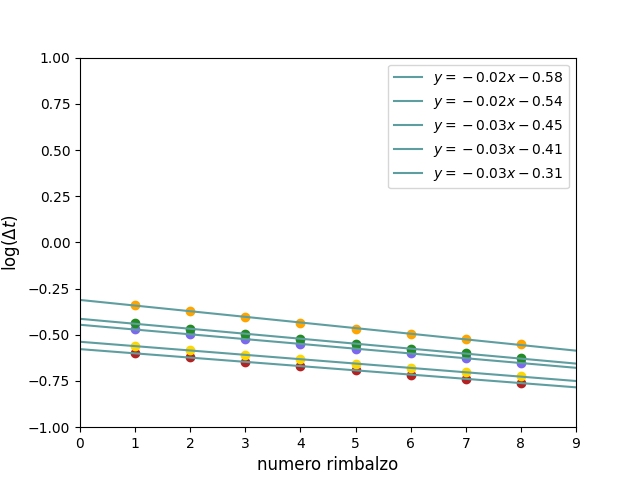
\includegraphics{Metodo2/computed_data/graficoLog_interpolato_pallina1.png}
			} %close resize
		} %close centering
		\caption{ Figura4: \(log\Delta t _{(n)}\) - pallina da ping pong - interpolazione}
	\end{figure}
	
	\noindent Così facendo si ottengono 5 stime del coefficiente di restituzione che possono essere combinate in una media pesata come \[\bar{e_{v}}=\frac{\sum\frac{e_{vi}}{\sigma_{i}^{2}}}{\sum\frac{1}{\sigma _{i}^{2}}} \pm \sqrt{\frac{1}{\sum \frac{1}{\sigma _{i}^{2}}}}\].
	
	\[\begin{matrix}
		$8cm:$ & $\(B = -0.0230 \pm 0.0001 \rightarrow\)$&$\(ev = 0.94848\pm0.00023\)$ &  \\ 
		$10cm:$ & $\(B = -0.02400\pm 0.00014\rightarrow\)$& $\(ev =0.9471 \pm 0.0003\)$ &  \\ 
		$15cm:$ & $\(B=-0.026 \pm 0.00009\rightarrow\)$&$\(ev = 0.94215\pm0.00019\)$ & $\(\qquad \Rightarrow \quad \bar{e_{v}} = 0.9423 \pm 0.0001\)$\\ 
		$18cm:$ & $\(B=-0.027\pm 0.00018\rightarrow\)$& $\(ev = 0.9399\pm0.0004\)$ &  \\ 
		$30cm:$ & $\(B=-0.030\pm 0.00012\rightarrow\)$&$\(ev =  0.9322\pm0.0003\)$ & 
	\end{matrix}\]
	dove \(e_{v}= 10^{B}\), \(\sigma_{ev} = \sigma_{B}10^{B}ln(10)\). Notiamo che questa stima è molto più precisa di quella ottenuta con il metodo 1.\\
	\[t = \frac{ \left |ev_{metodo1}  - ev_{metodo2} \right |}{\sqrt{\sigma_{1}^{2}+ \sigma_{2}^{2}}} = 3,6  \]
	\noindent \(\rightarrow\) la probabilità che la differenza sia dovuta solo ad errori casuali è inferiore al 0.3\(\%\) consideriamo non accettabile l'ipotesi di compatibilità delle due misure.
	\section*{pallina da tennis su gres porcellanato}
	\subsubsection*{metodo 1}
	%tabelle per la pallina 3
	Altezza di partenza : \(h_{0}\) = 65cm
	
	\begin{table}[!ht]
		\centering
		
        \begin{tabular}{c|*{10}{c}}
            \hline
            \hline
                \(h_{1}\) & 33.000 & 33.500 & 32.000 & 32.800 & 32.100 & 33.100 & 32.700 & 33.600 & 33.100 & 32.1 \\
            \hline
            
            \hline
            \hline
        \end{tabular}
        
	\end{table}
		\noindent Altezza di partenza : \(h_{0}\) = 55cm
		
	\begin{table}[!ht]
		\centering
		
        \begin{tabular}{c|*{11}{c}}
            \hline
            \hline
                \(h_{1}\) & 28.5 & 29.9 & 28.2 & 28.6 & 29.0 & 30.0 & 29.5 & 28.6 & 28.5 & 30.0 \\
            \hline
            \hline
        \end{tabular}
        
	\end{table}
	\noindent	Altezza di partenza : \(h_{0}\) = 45cm
		
	\begin{table}[!ht]
		\centering
		
        \begin{tabular}{c|*{10}{c}}
            \hline
            \hline
                \(h_{1}\) & 25.0 & 25.2 & 24.6 & 25.1 & 24.8 & 25.0 & 25.4 & 24.8 & 24.7 & 25.5 \\
            \hline
            
            \hline
            \hline
        \end{tabular}
        
	\end{table}
	\noindent	Altezza di partenza : \(h_{0}\) = 35cm
		
	\begin{table}[!ht]
		\centering
		
        \begin{tabular}{c|*{10}{c}}
            \hline
            \hline
                \(h_{1}\) & 19.5 & 20.5 & 19.4 & 19.8 & 19.0 & 20.4 & 19.4 & 19.8 & 20.3 & 19.5 \\
            \hline
            
            \hline
            \hline
        \end{tabular}
        
	\end{table}
	\noindent	Altezza di partenza : \(h_{0}\) = 25cm
			
	\begin{table}[!ht]
		\centering
		
        \begin{tabular}{c|*{10}{c}}
            \hline
            \hline
                \(h_{1}\) & 12.200 & 12.800 & 13.000 & 12.700 & 12.500 & 13.100 & 13.200 & 13.200 & 13.000 & 13.0 \\
            \hline
            
            \hline
            \hline
        \end{tabular}
        
	\end{table}
	
	\begin{figure}[!htbp]
		\captionsetup{labelformat=empty}
			\caption{pallina da tennis: media ed errore sulla media delle altezze \(h_{1}\):}
		\makebox[1 \textwidth][c]{       %centering table
			\begin{tabular}{c|c|c}
				
				\(h_{0}\) (cm) & media \(h_{1}\) (cm) & \(\sigma_{m}\) (cm)\\
				\hline
				
				25 & 12.87 &  0.102\\
				
				35 & 19.76 &  0.157\\
				
				45 & 25.01 & 0.094\\
				
				55 & 29.05 & 0.222\\
				
				65 & 32.8 & 0.182\\
				\hline
			\end{tabular}
		} %close centering
	\end{figure}
	.\\\\\\\\\\\\\\\\\\\\\\
	%grafico dei punti pallina3
	\begin{figure}[!htbp]
		\captionsetup{labelformat=empty}
		\makebox[1 \textwidth][c]{       %centering table
			\resizebox{0.7 \textwidth}{!}{   %resize table
				%%% Creator: Matplotlib, PGF backend
%%
%% To include the figure in your LaTeX document, write
%%   \input{<filename>.pgf}
%%
%% Make sure the required packages are loaded in your preamble
%%   \usepackage{pgf}
%%
%% and, on pdftex
%%   \usepackage[utf8]{inputenc}\DeclareUnicodeCharacter{2212}{-}
%%
%% or, on luatex and xetex
%%   \usepackage{unicode-math}
%%
%% Figures using additional raster images can only be included by \input if
%% they are in the same directory as the main LaTeX file. For loading figures
%% from other directories you can use the `import` package
%%   \usepackage{import}
%%
%% and then include the figures with
%%   \import{<path to file>}{<filename>.pgf}
%%
%% Matplotlib used the following preamble
%%   \usepackage{fontspec}
%%   \setmainfont{DejaVuSerif.ttf}[Path=C:/Users/giuly/AppData/Local/Programs/Python/Python39/Lib/site-packages/matplotlib/mpl-data/fonts/ttf/]
%%   \setsansfont{DejaVuSans.ttf}[Path=C:/Users/giuly/AppData/Local/Programs/Python/Python39/Lib/site-packages/matplotlib/mpl-data/fonts/ttf/]
%%   \setmonofont{DejaVuSansMono.ttf}[Path=C:/Users/giuly/AppData/Local/Programs/Python/Python39/Lib/site-packages/matplotlib/mpl-data/fonts/ttf/]
%%
\begingroup%
\makeatletter%
\begin{pgfpicture}%
\pgfpathrectangle{\pgfpointorigin}{\pgfqpoint{6.400000in}{4.800000in}}%
\pgfusepath{use as bounding box, clip}%
\begin{pgfscope}%
\pgfsetbuttcap%
\pgfsetmiterjoin%
\definecolor{currentfill}{rgb}{1.000000,1.000000,1.000000}%
\pgfsetfillcolor{currentfill}%
\pgfsetlinewidth{0.000000pt}%
\definecolor{currentstroke}{rgb}{1.000000,1.000000,1.000000}%
\pgfsetstrokecolor{currentstroke}%
\pgfsetdash{}{0pt}%
\pgfpathmoveto{\pgfqpoint{0.000000in}{0.000000in}}%
\pgfpathlineto{\pgfqpoint{6.400000in}{0.000000in}}%
\pgfpathlineto{\pgfqpoint{6.400000in}{4.800000in}}%
\pgfpathlineto{\pgfqpoint{0.000000in}{4.800000in}}%
\pgfpathclose%
\pgfusepath{fill}%
\end{pgfscope}%
\begin{pgfscope}%
\pgfsetbuttcap%
\pgfsetmiterjoin%
\definecolor{currentfill}{rgb}{1.000000,1.000000,1.000000}%
\pgfsetfillcolor{currentfill}%
\pgfsetlinewidth{0.000000pt}%
\definecolor{currentstroke}{rgb}{0.000000,0.000000,0.000000}%
\pgfsetstrokecolor{currentstroke}%
\pgfsetstrokeopacity{0.000000}%
\pgfsetdash{}{0pt}%
\pgfpathmoveto{\pgfqpoint{0.800000in}{0.528000in}}%
\pgfpathlineto{\pgfqpoint{5.760000in}{0.528000in}}%
\pgfpathlineto{\pgfqpoint{5.760000in}{4.224000in}}%
\pgfpathlineto{\pgfqpoint{0.800000in}{4.224000in}}%
\pgfpathclose%
\pgfusepath{fill}%
\end{pgfscope}%
\begin{pgfscope}%
\pgfpathrectangle{\pgfqpoint{0.800000in}{0.528000in}}{\pgfqpoint{4.960000in}{3.696000in}}%
\pgfusepath{clip}%
\pgfsetbuttcap%
\pgfsetmiterjoin%
\definecolor{currentfill}{rgb}{0.400000,0.803922,0.666667}%
\pgfsetfillcolor{currentfill}%
\pgfsetfillopacity{0.800000}%
\pgfsetlinewidth{0.000000pt}%
\definecolor{currentstroke}{rgb}{0.000000,0.000000,0.000000}%
\pgfsetstrokecolor{currentstroke}%
\pgfsetstrokeopacity{0.800000}%
\pgfsetdash{}{0pt}%
\pgfpathmoveto{\pgfqpoint{1.025455in}{0.528000in}}%
\pgfpathlineto{\pgfqpoint{1.401212in}{0.528000in}}%
\pgfpathlineto{\pgfqpoint{1.401212in}{0.848000in}}%
\pgfpathlineto{\pgfqpoint{1.025455in}{0.848000in}}%
\pgfpathclose%
\pgfusepath{fill}%
\end{pgfscope}%
\begin{pgfscope}%
\pgfpathrectangle{\pgfqpoint{0.800000in}{0.528000in}}{\pgfqpoint{4.960000in}{3.696000in}}%
\pgfusepath{clip}%
\pgfsetbuttcap%
\pgfsetmiterjoin%
\definecolor{currentfill}{rgb}{0.400000,0.803922,0.666667}%
\pgfsetfillcolor{currentfill}%
\pgfsetfillopacity{0.800000}%
\pgfsetlinewidth{0.000000pt}%
\definecolor{currentstroke}{rgb}{0.000000,0.000000,0.000000}%
\pgfsetstrokecolor{currentstroke}%
\pgfsetstrokeopacity{0.800000}%
\pgfsetdash{}{0pt}%
\pgfpathmoveto{\pgfqpoint{1.401212in}{0.528000in}}%
\pgfpathlineto{\pgfqpoint{1.776970in}{0.528000in}}%
\pgfpathlineto{\pgfqpoint{1.776970in}{0.848000in}}%
\pgfpathlineto{\pgfqpoint{1.401212in}{0.848000in}}%
\pgfpathclose%
\pgfusepath{fill}%
\end{pgfscope}%
\begin{pgfscope}%
\pgfpathrectangle{\pgfqpoint{0.800000in}{0.528000in}}{\pgfqpoint{4.960000in}{3.696000in}}%
\pgfusepath{clip}%
\pgfsetbuttcap%
\pgfsetmiterjoin%
\definecolor{currentfill}{rgb}{0.400000,0.803922,0.666667}%
\pgfsetfillcolor{currentfill}%
\pgfsetfillopacity{0.800000}%
\pgfsetlinewidth{0.000000pt}%
\definecolor{currentstroke}{rgb}{0.000000,0.000000,0.000000}%
\pgfsetstrokecolor{currentstroke}%
\pgfsetstrokeopacity{0.800000}%
\pgfsetdash{}{0pt}%
\pgfpathmoveto{\pgfqpoint{1.776970in}{0.528000in}}%
\pgfpathlineto{\pgfqpoint{2.152727in}{0.528000in}}%
\pgfpathlineto{\pgfqpoint{2.152727in}{1.168000in}}%
\pgfpathlineto{\pgfqpoint{1.776970in}{1.168000in}}%
\pgfpathclose%
\pgfusepath{fill}%
\end{pgfscope}%
\begin{pgfscope}%
\pgfpathrectangle{\pgfqpoint{0.800000in}{0.528000in}}{\pgfqpoint{4.960000in}{3.696000in}}%
\pgfusepath{clip}%
\pgfsetbuttcap%
\pgfsetmiterjoin%
\definecolor{currentfill}{rgb}{0.400000,0.803922,0.666667}%
\pgfsetfillcolor{currentfill}%
\pgfsetfillopacity{0.800000}%
\pgfsetlinewidth{0.000000pt}%
\definecolor{currentstroke}{rgb}{0.000000,0.000000,0.000000}%
\pgfsetstrokecolor{currentstroke}%
\pgfsetstrokeopacity{0.800000}%
\pgfsetdash{}{0pt}%
\pgfpathmoveto{\pgfqpoint{2.152727in}{0.528000in}}%
\pgfpathlineto{\pgfqpoint{2.528485in}{0.528000in}}%
\pgfpathlineto{\pgfqpoint{2.528485in}{1.968000in}}%
\pgfpathlineto{\pgfqpoint{2.152727in}{1.968000in}}%
\pgfpathclose%
\pgfusepath{fill}%
\end{pgfscope}%
\begin{pgfscope}%
\pgfpathrectangle{\pgfqpoint{0.800000in}{0.528000in}}{\pgfqpoint{4.960000in}{3.696000in}}%
\pgfusepath{clip}%
\pgfsetbuttcap%
\pgfsetmiterjoin%
\definecolor{currentfill}{rgb}{0.400000,0.803922,0.666667}%
\pgfsetfillcolor{currentfill}%
\pgfsetfillopacity{0.800000}%
\pgfsetlinewidth{0.000000pt}%
\definecolor{currentstroke}{rgb}{0.000000,0.000000,0.000000}%
\pgfsetstrokecolor{currentstroke}%
\pgfsetstrokeopacity{0.800000}%
\pgfsetdash{}{0pt}%
\pgfpathmoveto{\pgfqpoint{2.528485in}{0.528000in}}%
\pgfpathlineto{\pgfqpoint{2.904242in}{0.528000in}}%
\pgfpathlineto{\pgfqpoint{2.904242in}{2.448000in}}%
\pgfpathlineto{\pgfqpoint{2.528485in}{2.448000in}}%
\pgfpathclose%
\pgfusepath{fill}%
\end{pgfscope}%
\begin{pgfscope}%
\pgfpathrectangle{\pgfqpoint{0.800000in}{0.528000in}}{\pgfqpoint{4.960000in}{3.696000in}}%
\pgfusepath{clip}%
\pgfsetbuttcap%
\pgfsetmiterjoin%
\definecolor{currentfill}{rgb}{0.400000,0.803922,0.666667}%
\pgfsetfillcolor{currentfill}%
\pgfsetfillopacity{0.800000}%
\pgfsetlinewidth{0.000000pt}%
\definecolor{currentstroke}{rgb}{0.000000,0.000000,0.000000}%
\pgfsetstrokecolor{currentstroke}%
\pgfsetstrokeopacity{0.800000}%
\pgfsetdash{}{0pt}%
\pgfpathmoveto{\pgfqpoint{2.904242in}{0.528000in}}%
\pgfpathlineto{\pgfqpoint{3.280000in}{0.528000in}}%
\pgfpathlineto{\pgfqpoint{3.280000in}{4.048000in}}%
\pgfpathlineto{\pgfqpoint{2.904242in}{4.048000in}}%
\pgfpathclose%
\pgfusepath{fill}%
\end{pgfscope}%
\begin{pgfscope}%
\pgfpathrectangle{\pgfqpoint{0.800000in}{0.528000in}}{\pgfqpoint{4.960000in}{3.696000in}}%
\pgfusepath{clip}%
\pgfsetbuttcap%
\pgfsetmiterjoin%
\definecolor{currentfill}{rgb}{0.400000,0.803922,0.666667}%
\pgfsetfillcolor{currentfill}%
\pgfsetfillopacity{0.800000}%
\pgfsetlinewidth{0.000000pt}%
\definecolor{currentstroke}{rgb}{0.000000,0.000000,0.000000}%
\pgfsetstrokecolor{currentstroke}%
\pgfsetstrokeopacity{0.800000}%
\pgfsetdash{}{0pt}%
\pgfpathmoveto{\pgfqpoint{3.280000in}{0.528000in}}%
\pgfpathlineto{\pgfqpoint{3.655758in}{0.528000in}}%
\pgfpathlineto{\pgfqpoint{3.655758in}{3.248000in}}%
\pgfpathlineto{\pgfqpoint{3.280000in}{3.248000in}}%
\pgfpathclose%
\pgfusepath{fill}%
\end{pgfscope}%
\begin{pgfscope}%
\pgfpathrectangle{\pgfqpoint{0.800000in}{0.528000in}}{\pgfqpoint{4.960000in}{3.696000in}}%
\pgfusepath{clip}%
\pgfsetbuttcap%
\pgfsetmiterjoin%
\definecolor{currentfill}{rgb}{0.400000,0.803922,0.666667}%
\pgfsetfillcolor{currentfill}%
\pgfsetfillopacity{0.800000}%
\pgfsetlinewidth{0.000000pt}%
\definecolor{currentstroke}{rgb}{0.000000,0.000000,0.000000}%
\pgfsetstrokecolor{currentstroke}%
\pgfsetstrokeopacity{0.800000}%
\pgfsetdash{}{0pt}%
\pgfpathmoveto{\pgfqpoint{3.655758in}{0.528000in}}%
\pgfpathlineto{\pgfqpoint{4.031515in}{0.528000in}}%
\pgfpathlineto{\pgfqpoint{4.031515in}{3.248000in}}%
\pgfpathlineto{\pgfqpoint{3.655758in}{3.248000in}}%
\pgfpathclose%
\pgfusepath{fill}%
\end{pgfscope}%
\begin{pgfscope}%
\pgfpathrectangle{\pgfqpoint{0.800000in}{0.528000in}}{\pgfqpoint{4.960000in}{3.696000in}}%
\pgfusepath{clip}%
\pgfsetbuttcap%
\pgfsetmiterjoin%
\definecolor{currentfill}{rgb}{0.400000,0.803922,0.666667}%
\pgfsetfillcolor{currentfill}%
\pgfsetfillopacity{0.800000}%
\pgfsetlinewidth{0.000000pt}%
\definecolor{currentstroke}{rgb}{0.000000,0.000000,0.000000}%
\pgfsetstrokecolor{currentstroke}%
\pgfsetstrokeopacity{0.800000}%
\pgfsetdash{}{0pt}%
\pgfpathmoveto{\pgfqpoint{4.031515in}{0.528000in}}%
\pgfpathlineto{\pgfqpoint{4.407273in}{0.528000in}}%
\pgfpathlineto{\pgfqpoint{4.407273in}{1.968000in}}%
\pgfpathlineto{\pgfqpoint{4.031515in}{1.968000in}}%
\pgfpathclose%
\pgfusepath{fill}%
\end{pgfscope}%
\begin{pgfscope}%
\pgfpathrectangle{\pgfqpoint{0.800000in}{0.528000in}}{\pgfqpoint{4.960000in}{3.696000in}}%
\pgfusepath{clip}%
\pgfsetbuttcap%
\pgfsetmiterjoin%
\definecolor{currentfill}{rgb}{0.400000,0.803922,0.666667}%
\pgfsetfillcolor{currentfill}%
\pgfsetfillopacity{0.800000}%
\pgfsetlinewidth{0.000000pt}%
\definecolor{currentstroke}{rgb}{0.000000,0.000000,0.000000}%
\pgfsetstrokecolor{currentstroke}%
\pgfsetstrokeopacity{0.800000}%
\pgfsetdash{}{0pt}%
\pgfpathmoveto{\pgfqpoint{4.407273in}{0.528000in}}%
\pgfpathlineto{\pgfqpoint{4.783030in}{0.528000in}}%
\pgfpathlineto{\pgfqpoint{4.783030in}{1.168000in}}%
\pgfpathlineto{\pgfqpoint{4.407273in}{1.168000in}}%
\pgfpathclose%
\pgfusepath{fill}%
\end{pgfscope}%
\begin{pgfscope}%
\pgfpathrectangle{\pgfqpoint{0.800000in}{0.528000in}}{\pgfqpoint{4.960000in}{3.696000in}}%
\pgfusepath{clip}%
\pgfsetbuttcap%
\pgfsetmiterjoin%
\definecolor{currentfill}{rgb}{0.400000,0.803922,0.666667}%
\pgfsetfillcolor{currentfill}%
\pgfsetfillopacity{0.800000}%
\pgfsetlinewidth{0.000000pt}%
\definecolor{currentstroke}{rgb}{0.000000,0.000000,0.000000}%
\pgfsetstrokecolor{currentstroke}%
\pgfsetstrokeopacity{0.800000}%
\pgfsetdash{}{0pt}%
\pgfpathmoveto{\pgfqpoint{4.783030in}{0.528000in}}%
\pgfpathlineto{\pgfqpoint{5.158788in}{0.528000in}}%
\pgfpathlineto{\pgfqpoint{5.158788in}{0.688000in}}%
\pgfpathlineto{\pgfqpoint{4.783030in}{0.688000in}}%
\pgfpathclose%
\pgfusepath{fill}%
\end{pgfscope}%
\begin{pgfscope}%
\pgfpathrectangle{\pgfqpoint{0.800000in}{0.528000in}}{\pgfqpoint{4.960000in}{3.696000in}}%
\pgfusepath{clip}%
\pgfsetbuttcap%
\pgfsetmiterjoin%
\definecolor{currentfill}{rgb}{0.400000,0.803922,0.666667}%
\pgfsetfillcolor{currentfill}%
\pgfsetfillopacity{0.800000}%
\pgfsetlinewidth{0.000000pt}%
\definecolor{currentstroke}{rgb}{0.000000,0.000000,0.000000}%
\pgfsetstrokecolor{currentstroke}%
\pgfsetstrokeopacity{0.800000}%
\pgfsetdash{}{0pt}%
\pgfpathmoveto{\pgfqpoint{5.158788in}{0.528000in}}%
\pgfpathlineto{\pgfqpoint{5.534545in}{0.528000in}}%
\pgfpathlineto{\pgfqpoint{5.534545in}{0.688000in}}%
\pgfpathlineto{\pgfqpoint{5.158788in}{0.688000in}}%
\pgfpathclose%
\pgfusepath{fill}%
\end{pgfscope}%
\begin{pgfscope}%
\pgfsetbuttcap%
\pgfsetroundjoin%
\definecolor{currentfill}{rgb}{0.000000,0.000000,0.000000}%
\pgfsetfillcolor{currentfill}%
\pgfsetlinewidth{0.803000pt}%
\definecolor{currentstroke}{rgb}{0.000000,0.000000,0.000000}%
\pgfsetstrokecolor{currentstroke}%
\pgfsetdash{}{0pt}%
\pgfsys@defobject{currentmarker}{\pgfqpoint{0.000000in}{-0.048611in}}{\pgfqpoint{0.000000in}{0.000000in}}{%
\pgfpathmoveto{\pgfqpoint{0.000000in}{0.000000in}}%
\pgfpathlineto{\pgfqpoint{0.000000in}{-0.048611in}}%
\pgfusepath{stroke,fill}%
}%
\begin{pgfscope}%
\pgfsys@transformshift{1.025455in}{0.528000in}%
\pgfsys@useobject{currentmarker}{}%
\end{pgfscope}%
\end{pgfscope}%
\begin{pgfscope}%
\definecolor{textcolor}{rgb}{0.000000,0.000000,0.000000}%
\pgfsetstrokecolor{textcolor}%
\pgfsetfillcolor{textcolor}%
\pgftext[x=1.025455in,y=0.430778in,,top]{\color{textcolor}\sffamily\fontsize{10.000000}{12.000000}\selectfont 1.30}%
\end{pgfscope}%
\begin{pgfscope}%
\pgfsetbuttcap%
\pgfsetroundjoin%
\definecolor{currentfill}{rgb}{0.000000,0.000000,0.000000}%
\pgfsetfillcolor{currentfill}%
\pgfsetlinewidth{0.803000pt}%
\definecolor{currentstroke}{rgb}{0.000000,0.000000,0.000000}%
\pgfsetstrokecolor{currentstroke}%
\pgfsetdash{}{0pt}%
\pgfsys@defobject{currentmarker}{\pgfqpoint{0.000000in}{-0.048611in}}{\pgfqpoint{0.000000in}{0.000000in}}{%
\pgfpathmoveto{\pgfqpoint{0.000000in}{0.000000in}}%
\pgfpathlineto{\pgfqpoint{0.000000in}{-0.048611in}}%
\pgfusepath{stroke,fill}%
}%
\begin{pgfscope}%
\pgfsys@transformshift{1.589091in}{0.528000in}%
\pgfsys@useobject{currentmarker}{}%
\end{pgfscope}%
\end{pgfscope}%
\begin{pgfscope}%
\definecolor{textcolor}{rgb}{0.000000,0.000000,0.000000}%
\pgfsetstrokecolor{textcolor}%
\pgfsetfillcolor{textcolor}%
\pgftext[x=1.589091in,y=0.430778in,,top]{\color{textcolor}\sffamily\fontsize{10.000000}{12.000000}\selectfont 1.35}%
\end{pgfscope}%
\begin{pgfscope}%
\pgfsetbuttcap%
\pgfsetroundjoin%
\definecolor{currentfill}{rgb}{0.000000,0.000000,0.000000}%
\pgfsetfillcolor{currentfill}%
\pgfsetlinewidth{0.803000pt}%
\definecolor{currentstroke}{rgb}{0.000000,0.000000,0.000000}%
\pgfsetstrokecolor{currentstroke}%
\pgfsetdash{}{0pt}%
\pgfsys@defobject{currentmarker}{\pgfqpoint{0.000000in}{-0.048611in}}{\pgfqpoint{0.000000in}{0.000000in}}{%
\pgfpathmoveto{\pgfqpoint{0.000000in}{0.000000in}}%
\pgfpathlineto{\pgfqpoint{0.000000in}{-0.048611in}}%
\pgfusepath{stroke,fill}%
}%
\begin{pgfscope}%
\pgfsys@transformshift{2.152727in}{0.528000in}%
\pgfsys@useobject{currentmarker}{}%
\end{pgfscope}%
\end{pgfscope}%
\begin{pgfscope}%
\definecolor{textcolor}{rgb}{0.000000,0.000000,0.000000}%
\pgfsetstrokecolor{textcolor}%
\pgfsetfillcolor{textcolor}%
\pgftext[x=2.152727in,y=0.430778in,,top]{\color{textcolor}\sffamily\fontsize{10.000000}{12.000000}\selectfont 1.40}%
\end{pgfscope}%
\begin{pgfscope}%
\pgfsetbuttcap%
\pgfsetroundjoin%
\definecolor{currentfill}{rgb}{0.000000,0.000000,0.000000}%
\pgfsetfillcolor{currentfill}%
\pgfsetlinewidth{0.803000pt}%
\definecolor{currentstroke}{rgb}{0.000000,0.000000,0.000000}%
\pgfsetstrokecolor{currentstroke}%
\pgfsetdash{}{0pt}%
\pgfsys@defobject{currentmarker}{\pgfqpoint{0.000000in}{-0.048611in}}{\pgfqpoint{0.000000in}{0.000000in}}{%
\pgfpathmoveto{\pgfqpoint{0.000000in}{0.000000in}}%
\pgfpathlineto{\pgfqpoint{0.000000in}{-0.048611in}}%
\pgfusepath{stroke,fill}%
}%
\begin{pgfscope}%
\pgfsys@transformshift{2.716364in}{0.528000in}%
\pgfsys@useobject{currentmarker}{}%
\end{pgfscope}%
\end{pgfscope}%
\begin{pgfscope}%
\definecolor{textcolor}{rgb}{0.000000,0.000000,0.000000}%
\pgfsetstrokecolor{textcolor}%
\pgfsetfillcolor{textcolor}%
\pgftext[x=2.716364in,y=0.430778in,,top]{\color{textcolor}\sffamily\fontsize{10.000000}{12.000000}\selectfont 1.45}%
\end{pgfscope}%
\begin{pgfscope}%
\pgfsetbuttcap%
\pgfsetroundjoin%
\definecolor{currentfill}{rgb}{0.000000,0.000000,0.000000}%
\pgfsetfillcolor{currentfill}%
\pgfsetlinewidth{0.803000pt}%
\definecolor{currentstroke}{rgb}{0.000000,0.000000,0.000000}%
\pgfsetstrokecolor{currentstroke}%
\pgfsetdash{}{0pt}%
\pgfsys@defobject{currentmarker}{\pgfqpoint{0.000000in}{-0.048611in}}{\pgfqpoint{0.000000in}{0.000000in}}{%
\pgfpathmoveto{\pgfqpoint{0.000000in}{0.000000in}}%
\pgfpathlineto{\pgfqpoint{0.000000in}{-0.048611in}}%
\pgfusepath{stroke,fill}%
}%
\begin{pgfscope}%
\pgfsys@transformshift{3.280000in}{0.528000in}%
\pgfsys@useobject{currentmarker}{}%
\end{pgfscope}%
\end{pgfscope}%
\begin{pgfscope}%
\definecolor{textcolor}{rgb}{0.000000,0.000000,0.000000}%
\pgfsetstrokecolor{textcolor}%
\pgfsetfillcolor{textcolor}%
\pgftext[x=3.280000in,y=0.430778in,,top]{\color{textcolor}\sffamily\fontsize{10.000000}{12.000000}\selectfont 1.50}%
\end{pgfscope}%
\begin{pgfscope}%
\pgfsetbuttcap%
\pgfsetroundjoin%
\definecolor{currentfill}{rgb}{0.000000,0.000000,0.000000}%
\pgfsetfillcolor{currentfill}%
\pgfsetlinewidth{0.803000pt}%
\definecolor{currentstroke}{rgb}{0.000000,0.000000,0.000000}%
\pgfsetstrokecolor{currentstroke}%
\pgfsetdash{}{0pt}%
\pgfsys@defobject{currentmarker}{\pgfqpoint{0.000000in}{-0.048611in}}{\pgfqpoint{0.000000in}{0.000000in}}{%
\pgfpathmoveto{\pgfqpoint{0.000000in}{0.000000in}}%
\pgfpathlineto{\pgfqpoint{0.000000in}{-0.048611in}}%
\pgfusepath{stroke,fill}%
}%
\begin{pgfscope}%
\pgfsys@transformshift{3.843636in}{0.528000in}%
\pgfsys@useobject{currentmarker}{}%
\end{pgfscope}%
\end{pgfscope}%
\begin{pgfscope}%
\definecolor{textcolor}{rgb}{0.000000,0.000000,0.000000}%
\pgfsetstrokecolor{textcolor}%
\pgfsetfillcolor{textcolor}%
\pgftext[x=3.843636in,y=0.430778in,,top]{\color{textcolor}\sffamily\fontsize{10.000000}{12.000000}\selectfont 1.55}%
\end{pgfscope}%
\begin{pgfscope}%
\pgfsetbuttcap%
\pgfsetroundjoin%
\definecolor{currentfill}{rgb}{0.000000,0.000000,0.000000}%
\pgfsetfillcolor{currentfill}%
\pgfsetlinewidth{0.803000pt}%
\definecolor{currentstroke}{rgb}{0.000000,0.000000,0.000000}%
\pgfsetstrokecolor{currentstroke}%
\pgfsetdash{}{0pt}%
\pgfsys@defobject{currentmarker}{\pgfqpoint{0.000000in}{-0.048611in}}{\pgfqpoint{0.000000in}{0.000000in}}{%
\pgfpathmoveto{\pgfqpoint{0.000000in}{0.000000in}}%
\pgfpathlineto{\pgfqpoint{0.000000in}{-0.048611in}}%
\pgfusepath{stroke,fill}%
}%
\begin{pgfscope}%
\pgfsys@transformshift{4.407273in}{0.528000in}%
\pgfsys@useobject{currentmarker}{}%
\end{pgfscope}%
\end{pgfscope}%
\begin{pgfscope}%
\definecolor{textcolor}{rgb}{0.000000,0.000000,0.000000}%
\pgfsetstrokecolor{textcolor}%
\pgfsetfillcolor{textcolor}%
\pgftext[x=4.407273in,y=0.430778in,,top]{\color{textcolor}\sffamily\fontsize{10.000000}{12.000000}\selectfont 1.60}%
\end{pgfscope}%
\begin{pgfscope}%
\pgfsetbuttcap%
\pgfsetroundjoin%
\definecolor{currentfill}{rgb}{0.000000,0.000000,0.000000}%
\pgfsetfillcolor{currentfill}%
\pgfsetlinewidth{0.803000pt}%
\definecolor{currentstroke}{rgb}{0.000000,0.000000,0.000000}%
\pgfsetstrokecolor{currentstroke}%
\pgfsetdash{}{0pt}%
\pgfsys@defobject{currentmarker}{\pgfqpoint{0.000000in}{-0.048611in}}{\pgfqpoint{0.000000in}{0.000000in}}{%
\pgfpathmoveto{\pgfqpoint{0.000000in}{0.000000in}}%
\pgfpathlineto{\pgfqpoint{0.000000in}{-0.048611in}}%
\pgfusepath{stroke,fill}%
}%
\begin{pgfscope}%
\pgfsys@transformshift{4.970909in}{0.528000in}%
\pgfsys@useobject{currentmarker}{}%
\end{pgfscope}%
\end{pgfscope}%
\begin{pgfscope}%
\definecolor{textcolor}{rgb}{0.000000,0.000000,0.000000}%
\pgfsetstrokecolor{textcolor}%
\pgfsetfillcolor{textcolor}%
\pgftext[x=4.970909in,y=0.430778in,,top]{\color{textcolor}\sffamily\fontsize{10.000000}{12.000000}\selectfont 1.65}%
\end{pgfscope}%
\begin{pgfscope}%
\pgfsetbuttcap%
\pgfsetroundjoin%
\definecolor{currentfill}{rgb}{0.000000,0.000000,0.000000}%
\pgfsetfillcolor{currentfill}%
\pgfsetlinewidth{0.803000pt}%
\definecolor{currentstroke}{rgb}{0.000000,0.000000,0.000000}%
\pgfsetstrokecolor{currentstroke}%
\pgfsetdash{}{0pt}%
\pgfsys@defobject{currentmarker}{\pgfqpoint{0.000000in}{-0.048611in}}{\pgfqpoint{0.000000in}{0.000000in}}{%
\pgfpathmoveto{\pgfqpoint{0.000000in}{0.000000in}}%
\pgfpathlineto{\pgfqpoint{0.000000in}{-0.048611in}}%
\pgfusepath{stroke,fill}%
}%
\begin{pgfscope}%
\pgfsys@transformshift{5.534545in}{0.528000in}%
\pgfsys@useobject{currentmarker}{}%
\end{pgfscope}%
\end{pgfscope}%
\begin{pgfscope}%
\definecolor{textcolor}{rgb}{0.000000,0.000000,0.000000}%
\pgfsetstrokecolor{textcolor}%
\pgfsetfillcolor{textcolor}%
\pgftext[x=5.534545in,y=0.430778in,,top]{\color{textcolor}\sffamily\fontsize{10.000000}{12.000000}\selectfont 1.70}%
\end{pgfscope}%
\begin{pgfscope}%
\definecolor{textcolor}{rgb}{0.000000,0.000000,0.000000}%
\pgfsetstrokecolor{textcolor}%
\pgfsetfillcolor{textcolor}%
\pgftext[x=3.280000in,y=0.240809in,,top]{\color{textcolor}\sffamily\fontsize{10.000000}{12.000000}\selectfont \(\displaystyle x_k\) (s)}%
\end{pgfscope}%
\begin{pgfscope}%
\pgfsetbuttcap%
\pgfsetroundjoin%
\definecolor{currentfill}{rgb}{0.000000,0.000000,0.000000}%
\pgfsetfillcolor{currentfill}%
\pgfsetlinewidth{0.803000pt}%
\definecolor{currentstroke}{rgb}{0.000000,0.000000,0.000000}%
\pgfsetstrokecolor{currentstroke}%
\pgfsetdash{}{0pt}%
\pgfsys@defobject{currentmarker}{\pgfqpoint{-0.048611in}{0.000000in}}{\pgfqpoint{-0.000000in}{0.000000in}}{%
\pgfpathmoveto{\pgfqpoint{-0.000000in}{0.000000in}}%
\pgfpathlineto{\pgfqpoint{-0.048611in}{0.000000in}}%
\pgfusepath{stroke,fill}%
}%
\begin{pgfscope}%
\pgfsys@transformshift{0.800000in}{0.528000in}%
\pgfsys@useobject{currentmarker}{}%
\end{pgfscope}%
\end{pgfscope}%
\begin{pgfscope}%
\definecolor{textcolor}{rgb}{0.000000,0.000000,0.000000}%
\pgfsetstrokecolor{textcolor}%
\pgfsetfillcolor{textcolor}%
\pgftext[x=0.614412in, y=0.475238in, left, base]{\color{textcolor}\sffamily\fontsize{10.000000}{12.000000}\selectfont 0}%
\end{pgfscope}%
\begin{pgfscope}%
\pgfsetbuttcap%
\pgfsetroundjoin%
\definecolor{currentfill}{rgb}{0.000000,0.000000,0.000000}%
\pgfsetfillcolor{currentfill}%
\pgfsetlinewidth{0.803000pt}%
\definecolor{currentstroke}{rgb}{0.000000,0.000000,0.000000}%
\pgfsetstrokecolor{currentstroke}%
\pgfsetdash{}{0pt}%
\pgfsys@defobject{currentmarker}{\pgfqpoint{-0.048611in}{0.000000in}}{\pgfqpoint{-0.000000in}{0.000000in}}{%
\pgfpathmoveto{\pgfqpoint{-0.000000in}{0.000000in}}%
\pgfpathlineto{\pgfqpoint{-0.048611in}{0.000000in}}%
\pgfusepath{stroke,fill}%
}%
\begin{pgfscope}%
\pgfsys@transformshift{0.800000in}{1.061333in}%
\pgfsys@useobject{currentmarker}{}%
\end{pgfscope}%
\end{pgfscope}%
\begin{pgfscope}%
\definecolor{textcolor}{rgb}{0.000000,0.000000,0.000000}%
\pgfsetstrokecolor{textcolor}%
\pgfsetfillcolor{textcolor}%
\pgftext[x=0.614412in, y=1.008572in, left, base]{\color{textcolor}\sffamily\fontsize{10.000000}{12.000000}\selectfont 1}%
\end{pgfscope}%
\begin{pgfscope}%
\pgfsetbuttcap%
\pgfsetroundjoin%
\definecolor{currentfill}{rgb}{0.000000,0.000000,0.000000}%
\pgfsetfillcolor{currentfill}%
\pgfsetlinewidth{0.803000pt}%
\definecolor{currentstroke}{rgb}{0.000000,0.000000,0.000000}%
\pgfsetstrokecolor{currentstroke}%
\pgfsetdash{}{0pt}%
\pgfsys@defobject{currentmarker}{\pgfqpoint{-0.048611in}{0.000000in}}{\pgfqpoint{-0.000000in}{0.000000in}}{%
\pgfpathmoveto{\pgfqpoint{-0.000000in}{0.000000in}}%
\pgfpathlineto{\pgfqpoint{-0.048611in}{0.000000in}}%
\pgfusepath{stroke,fill}%
}%
\begin{pgfscope}%
\pgfsys@transformshift{0.800000in}{1.594667in}%
\pgfsys@useobject{currentmarker}{}%
\end{pgfscope}%
\end{pgfscope}%
\begin{pgfscope}%
\definecolor{textcolor}{rgb}{0.000000,0.000000,0.000000}%
\pgfsetstrokecolor{textcolor}%
\pgfsetfillcolor{textcolor}%
\pgftext[x=0.614412in, y=1.541905in, left, base]{\color{textcolor}\sffamily\fontsize{10.000000}{12.000000}\selectfont 2}%
\end{pgfscope}%
\begin{pgfscope}%
\pgfsetbuttcap%
\pgfsetroundjoin%
\definecolor{currentfill}{rgb}{0.000000,0.000000,0.000000}%
\pgfsetfillcolor{currentfill}%
\pgfsetlinewidth{0.803000pt}%
\definecolor{currentstroke}{rgb}{0.000000,0.000000,0.000000}%
\pgfsetstrokecolor{currentstroke}%
\pgfsetdash{}{0pt}%
\pgfsys@defobject{currentmarker}{\pgfqpoint{-0.048611in}{0.000000in}}{\pgfqpoint{-0.000000in}{0.000000in}}{%
\pgfpathmoveto{\pgfqpoint{-0.000000in}{0.000000in}}%
\pgfpathlineto{\pgfqpoint{-0.048611in}{0.000000in}}%
\pgfusepath{stroke,fill}%
}%
\begin{pgfscope}%
\pgfsys@transformshift{0.800000in}{2.128000in}%
\pgfsys@useobject{currentmarker}{}%
\end{pgfscope}%
\end{pgfscope}%
\begin{pgfscope}%
\definecolor{textcolor}{rgb}{0.000000,0.000000,0.000000}%
\pgfsetstrokecolor{textcolor}%
\pgfsetfillcolor{textcolor}%
\pgftext[x=0.614412in, y=2.075238in, left, base]{\color{textcolor}\sffamily\fontsize{10.000000}{12.000000}\selectfont 3}%
\end{pgfscope}%
\begin{pgfscope}%
\pgfsetbuttcap%
\pgfsetroundjoin%
\definecolor{currentfill}{rgb}{0.000000,0.000000,0.000000}%
\pgfsetfillcolor{currentfill}%
\pgfsetlinewidth{0.803000pt}%
\definecolor{currentstroke}{rgb}{0.000000,0.000000,0.000000}%
\pgfsetstrokecolor{currentstroke}%
\pgfsetdash{}{0pt}%
\pgfsys@defobject{currentmarker}{\pgfqpoint{-0.048611in}{0.000000in}}{\pgfqpoint{-0.000000in}{0.000000in}}{%
\pgfpathmoveto{\pgfqpoint{-0.000000in}{0.000000in}}%
\pgfpathlineto{\pgfqpoint{-0.048611in}{0.000000in}}%
\pgfusepath{stroke,fill}%
}%
\begin{pgfscope}%
\pgfsys@transformshift{0.800000in}{2.661333in}%
\pgfsys@useobject{currentmarker}{}%
\end{pgfscope}%
\end{pgfscope}%
\begin{pgfscope}%
\definecolor{textcolor}{rgb}{0.000000,0.000000,0.000000}%
\pgfsetstrokecolor{textcolor}%
\pgfsetfillcolor{textcolor}%
\pgftext[x=0.614412in, y=2.608572in, left, base]{\color{textcolor}\sffamily\fontsize{10.000000}{12.000000}\selectfont 4}%
\end{pgfscope}%
\begin{pgfscope}%
\pgfsetbuttcap%
\pgfsetroundjoin%
\definecolor{currentfill}{rgb}{0.000000,0.000000,0.000000}%
\pgfsetfillcolor{currentfill}%
\pgfsetlinewidth{0.803000pt}%
\definecolor{currentstroke}{rgb}{0.000000,0.000000,0.000000}%
\pgfsetstrokecolor{currentstroke}%
\pgfsetdash{}{0pt}%
\pgfsys@defobject{currentmarker}{\pgfqpoint{-0.048611in}{0.000000in}}{\pgfqpoint{-0.000000in}{0.000000in}}{%
\pgfpathmoveto{\pgfqpoint{-0.000000in}{0.000000in}}%
\pgfpathlineto{\pgfqpoint{-0.048611in}{0.000000in}}%
\pgfusepath{stroke,fill}%
}%
\begin{pgfscope}%
\pgfsys@transformshift{0.800000in}{3.194667in}%
\pgfsys@useobject{currentmarker}{}%
\end{pgfscope}%
\end{pgfscope}%
\begin{pgfscope}%
\definecolor{textcolor}{rgb}{0.000000,0.000000,0.000000}%
\pgfsetstrokecolor{textcolor}%
\pgfsetfillcolor{textcolor}%
\pgftext[x=0.614412in, y=3.141905in, left, base]{\color{textcolor}\sffamily\fontsize{10.000000}{12.000000}\selectfont 5}%
\end{pgfscope}%
\begin{pgfscope}%
\pgfsetbuttcap%
\pgfsetroundjoin%
\definecolor{currentfill}{rgb}{0.000000,0.000000,0.000000}%
\pgfsetfillcolor{currentfill}%
\pgfsetlinewidth{0.803000pt}%
\definecolor{currentstroke}{rgb}{0.000000,0.000000,0.000000}%
\pgfsetstrokecolor{currentstroke}%
\pgfsetdash{}{0pt}%
\pgfsys@defobject{currentmarker}{\pgfqpoint{-0.048611in}{0.000000in}}{\pgfqpoint{-0.000000in}{0.000000in}}{%
\pgfpathmoveto{\pgfqpoint{-0.000000in}{0.000000in}}%
\pgfpathlineto{\pgfqpoint{-0.048611in}{0.000000in}}%
\pgfusepath{stroke,fill}%
}%
\begin{pgfscope}%
\pgfsys@transformshift{0.800000in}{3.728000in}%
\pgfsys@useobject{currentmarker}{}%
\end{pgfscope}%
\end{pgfscope}%
\begin{pgfscope}%
\definecolor{textcolor}{rgb}{0.000000,0.000000,0.000000}%
\pgfsetstrokecolor{textcolor}%
\pgfsetfillcolor{textcolor}%
\pgftext[x=0.614412in, y=3.675238in, left, base]{\color{textcolor}\sffamily\fontsize{10.000000}{12.000000}\selectfont 6}%
\end{pgfscope}%
\begin{pgfscope}%
\definecolor{textcolor}{rgb}{0.000000,0.000000,0.000000}%
\pgfsetstrokecolor{textcolor}%
\pgfsetfillcolor{textcolor}%
\pgftext[x=0.558857in,y=2.376000in,,bottom,rotate=90.000000]{\color{textcolor}\sffamily\fontsize{10.000000}{12.000000}\selectfont Densità di Frequenza}%
\end{pgfscope}%
\begin{pgfscope}%
\pgfpathrectangle{\pgfqpoint{0.800000in}{0.528000in}}{\pgfqpoint{4.960000in}{3.696000in}}%
\pgfusepath{clip}%
\pgfsetrectcap%
\pgfsetroundjoin%
\pgfsetlinewidth{1.505625pt}%
\definecolor{currentstroke}{rgb}{1.000000,0.549020,0.000000}%
\pgfsetstrokecolor{currentstroke}%
\pgfsetdash{}{0pt}%
\pgfpathmoveto{\pgfqpoint{1.025455in}{0.574044in}}%
\pgfpathlineto{\pgfqpoint{1.117477in}{0.593003in}}%
\pgfpathlineto{\pgfqpoint{1.209499in}{0.618431in}}%
\pgfpathlineto{\pgfqpoint{1.301521in}{0.651974in}}%
\pgfpathlineto{\pgfqpoint{1.393544in}{0.695485in}}%
\pgfpathlineto{\pgfqpoint{1.485566in}{0.750973in}}%
\pgfpathlineto{\pgfqpoint{1.577588in}{0.820521in}}%
\pgfpathlineto{\pgfqpoint{1.669610in}{0.906175in}}%
\pgfpathlineto{\pgfqpoint{1.761633in}{1.009791in}}%
\pgfpathlineto{\pgfqpoint{1.853655in}{1.132860in}}%
\pgfpathlineto{\pgfqpoint{1.945677in}{1.276309in}}%
\pgfpathlineto{\pgfqpoint{2.037699in}{1.440300in}}%
\pgfpathlineto{\pgfqpoint{2.129722in}{1.624034in}}%
\pgfpathlineto{\pgfqpoint{2.221744in}{1.825600in}}%
\pgfpathlineto{\pgfqpoint{2.313766in}{2.041867in}}%
\pgfpathlineto{\pgfqpoint{2.405788in}{2.268464in}}%
\pgfpathlineto{\pgfqpoint{2.497811in}{2.499842in}}%
\pgfpathlineto{\pgfqpoint{2.589833in}{2.729454in}}%
\pgfpathlineto{\pgfqpoint{2.681855in}{2.950017in}}%
\pgfpathlineto{\pgfqpoint{2.773878in}{3.153881in}}%
\pgfpathlineto{\pgfqpoint{2.865900in}{3.333452in}}%
\pgfpathlineto{\pgfqpoint{2.957922in}{3.481663in}}%
\pgfpathlineto{\pgfqpoint{3.049944in}{3.592427in}}%
\pgfpathlineto{\pgfqpoint{3.141967in}{3.661053in}}%
\pgfpathlineto{\pgfqpoint{3.233989in}{3.684577in}}%
\pgfpathlineto{\pgfqpoint{3.326011in}{3.661972in}}%
\pgfpathlineto{\pgfqpoint{3.418033in}{3.594225in}}%
\pgfpathlineto{\pgfqpoint{3.510056in}{3.484264in}}%
\pgfpathlineto{\pgfqpoint{3.602078in}{3.336746in}}%
\pgfpathlineto{\pgfqpoint{3.694100in}{3.157735in}}%
\pgfpathlineto{\pgfqpoint{3.786122in}{2.954284in}}%
\pgfpathlineto{\pgfqpoint{3.878145in}{2.733979in}}%
\pgfpathlineto{\pgfqpoint{3.970167in}{2.504475in}}%
\pgfpathlineto{\pgfqpoint{4.062189in}{2.273065in}}%
\pgfpathlineto{\pgfqpoint{4.154212in}{2.046315in}}%
\pgfpathlineto{\pgfqpoint{4.246234in}{1.829794in}}%
\pgfpathlineto{\pgfqpoint{4.338256in}{1.627899in}}%
\pgfpathlineto{\pgfqpoint{4.430278in}{1.443785in}}%
\pgfpathlineto{\pgfqpoint{4.522301in}{1.279389in}}%
\pgfpathlineto{\pgfqpoint{4.614323in}{1.135527in}}%
\pgfpathlineto{\pgfqpoint{4.706345in}{1.012058in}}%
\pgfpathlineto{\pgfqpoint{4.798367in}{0.908066in}}%
\pgfpathlineto{\pgfqpoint{4.890390in}{0.822070in}}%
\pgfpathlineto{\pgfqpoint{4.982412in}{0.752219in}}%
\pgfpathlineto{\pgfqpoint{5.074434in}{0.696471in}}%
\pgfpathlineto{\pgfqpoint{5.166456in}{0.652740in}}%
\pgfpathlineto{\pgfqpoint{5.258479in}{0.619016in}}%
\pgfpathlineto{\pgfqpoint{5.350501in}{0.593443in}}%
\pgfpathlineto{\pgfqpoint{5.442523in}{0.574370in}}%
\pgfpathlineto{\pgfqpoint{5.534545in}{0.560377in}}%
\pgfusepath{stroke}%
\end{pgfscope}%
\begin{pgfscope}%
\pgfsetrectcap%
\pgfsetmiterjoin%
\pgfsetlinewidth{0.803000pt}%
\definecolor{currentstroke}{rgb}{0.000000,0.000000,0.000000}%
\pgfsetstrokecolor{currentstroke}%
\pgfsetdash{}{0pt}%
\pgfpathmoveto{\pgfqpoint{0.800000in}{0.528000in}}%
\pgfpathlineto{\pgfqpoint{0.800000in}{4.224000in}}%
\pgfusepath{stroke}%
\end{pgfscope}%
\begin{pgfscope}%
\pgfsetrectcap%
\pgfsetmiterjoin%
\pgfsetlinewidth{0.803000pt}%
\definecolor{currentstroke}{rgb}{0.000000,0.000000,0.000000}%
\pgfsetstrokecolor{currentstroke}%
\pgfsetdash{}{0pt}%
\pgfpathmoveto{\pgfqpoint{5.760000in}{0.528000in}}%
\pgfpathlineto{\pgfqpoint{5.760000in}{4.224000in}}%
\pgfusepath{stroke}%
\end{pgfscope}%
\begin{pgfscope}%
\pgfsetrectcap%
\pgfsetmiterjoin%
\pgfsetlinewidth{0.803000pt}%
\definecolor{currentstroke}{rgb}{0.000000,0.000000,0.000000}%
\pgfsetstrokecolor{currentstroke}%
\pgfsetdash{}{0pt}%
\pgfpathmoveto{\pgfqpoint{0.800000in}{0.528000in}}%
\pgfpathlineto{\pgfqpoint{5.760000in}{0.528000in}}%
\pgfusepath{stroke}%
\end{pgfscope}%
\begin{pgfscope}%
\pgfsetrectcap%
\pgfsetmiterjoin%
\pgfsetlinewidth{0.803000pt}%
\definecolor{currentstroke}{rgb}{0.000000,0.000000,0.000000}%
\pgfsetstrokecolor{currentstroke}%
\pgfsetdash{}{0pt}%
\pgfpathmoveto{\pgfqpoint{0.800000in}{4.224000in}}%
\pgfpathlineto{\pgfqpoint{5.760000in}{4.224000in}}%
\pgfusepath{stroke}%
\end{pgfscope}%
\begin{pgfscope}%
\pgfsetbuttcap%
\pgfsetmiterjoin%
\definecolor{currentfill}{rgb}{1.000000,1.000000,1.000000}%
\pgfsetfillcolor{currentfill}%
\pgfsetfillopacity{0.800000}%
\pgfsetlinewidth{1.003750pt}%
\definecolor{currentstroke}{rgb}{0.800000,0.800000,0.800000}%
\pgfsetstrokecolor{currentstroke}%
\pgfsetstrokeopacity{0.800000}%
\pgfsetdash{}{0pt}%
\pgfpathmoveto{\pgfqpoint{4.613473in}{3.690899in}}%
\pgfpathlineto{\pgfqpoint{5.662778in}{3.690899in}}%
\pgfpathquadraticcurveto{\pgfqpoint{5.690556in}{3.690899in}}{\pgfqpoint{5.690556in}{3.718677in}}%
\pgfpathlineto{\pgfqpoint{5.690556in}{4.126778in}}%
\pgfpathquadraticcurveto{\pgfqpoint{5.690556in}{4.154556in}}{\pgfqpoint{5.662778in}{4.154556in}}%
\pgfpathlineto{\pgfqpoint{4.613473in}{4.154556in}}%
\pgfpathquadraticcurveto{\pgfqpoint{4.585695in}{4.154556in}}{\pgfqpoint{4.585695in}{4.126778in}}%
\pgfpathlineto{\pgfqpoint{4.585695in}{3.718677in}}%
\pgfpathquadraticcurveto{\pgfqpoint{4.585695in}{3.690899in}}{\pgfqpoint{4.613473in}{3.690899in}}%
\pgfpathclose%
\pgfusepath{stroke,fill}%
\end{pgfscope}%
\begin{pgfscope}%
\pgfsetrectcap%
\pgfsetroundjoin%
\pgfsetlinewidth{1.505625pt}%
\definecolor{currentstroke}{rgb}{1.000000,0.549020,0.000000}%
\pgfsetstrokecolor{currentstroke}%
\pgfsetdash{}{0pt}%
\pgfpathmoveto{\pgfqpoint{4.641251in}{4.033645in}}%
\pgfpathlineto{\pgfqpoint{4.919029in}{4.033645in}}%
\pgfusepath{stroke}%
\end{pgfscope}%
\begin{pgfscope}%
\definecolor{textcolor}{rgb}{0.000000,0.000000,0.000000}%
\pgfsetstrokecolor{textcolor}%
\pgfsetfillcolor{textcolor}%
\pgftext[x=5.030140in,y=3.985034in,left,base]{\color{textcolor}\sffamily\fontsize{10.000000}{12.000000}\selectfont \(\displaystyle G(x;\bar{T},\sigma)\)}%
\end{pgfscope}%
\begin{pgfscope}%
\pgfsetbuttcap%
\pgfsetmiterjoin%
\definecolor{currentfill}{rgb}{0.400000,0.803922,0.666667}%
\pgfsetfillcolor{currentfill}%
\pgfsetfillopacity{0.800000}%
\pgfsetlinewidth{0.000000pt}%
\definecolor{currentstroke}{rgb}{0.000000,0.000000,0.000000}%
\pgfsetstrokecolor{currentstroke}%
\pgfsetstrokeopacity{0.800000}%
\pgfsetdash{}{0pt}%
\pgfpathmoveto{\pgfqpoint{4.641251in}{3.775344in}}%
\pgfpathlineto{\pgfqpoint{4.919029in}{3.775344in}}%
\pgfpathlineto{\pgfqpoint{4.919029in}{3.872567in}}%
\pgfpathlineto{\pgfqpoint{4.641251in}{3.872567in}}%
\pgfpathclose%
\pgfusepath{fill}%
\end{pgfscope}%
\begin{pgfscope}%
\definecolor{textcolor}{rgb}{0.000000,0.000000,0.000000}%
\pgfsetstrokecolor{textcolor}%
\pgfsetfillcolor{textcolor}%
\pgftext[x=5.030140in,y=3.775344in,left,base]{\color{textcolor}\sffamily\fontsize{10.000000}{12.000000}\selectfont data}%
\end{pgfscope}%
\end{pgfpicture}%
\makeatother%
\endgroup%

				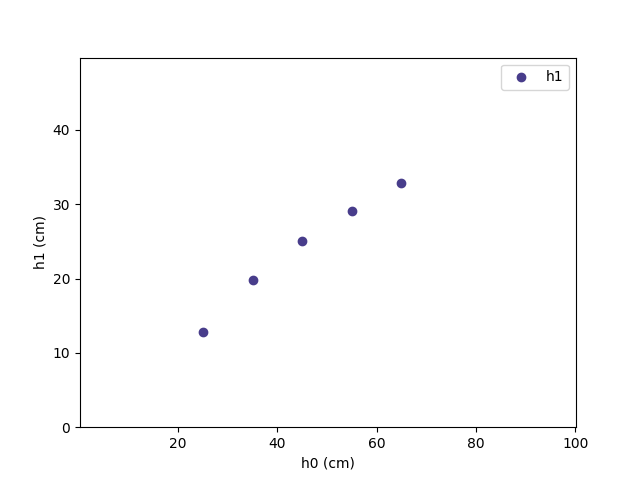
\includegraphics{Metodo1/computed_data/zoom_pallina3.png}
			} %close resize
		} %close centering
	\caption{Figura5: \(h1_{(h_{0})}\) - pallina da tennis su gres porcellanato}
	\end{figure}

	\noindent Interpolazione con il metodo dei minimi quadrati pesati:\\
	\[ con\quad\Delta = N(\sum \frac{x_{i}^{2}}{\sigma _{y_{i}}^{2}})-(\sum \frac{x_{i}}{\sigma _{y_{i}}^{2}})^{2}\]\\
	\[B = \frac{N(\sum\frac{x_{i}y_{i}}{\sigma _{y_{i}}^{2}})-\sum\frac{x_{i}}{\sigma _{y_{i}}^{2}}\sum\frac{y_{i}}{\sigma _{y_{i}}^{2}}}{\Delta } \quad
	\sigma _{B} = \sqrt{\frac{\sum \frac{1}{\sigma _{y_{i}}^{2}}}{\Delta}} \qquad
	\Rightarrow \qquad B = 0.524 \pm 0.005\]\\
	\[A = \frac{\sum \frac{(x_{i})^{2}}{\sigma _{y_{i}}^{2}}\sum \frac{(y_{i})^{2}}{\sigma _{y_{i}}^{2}}-\sum \frac{x_{i}}{\sigma _{y_{i}}^{2}}\sum \frac{x_{i}y_{i}}{\sigma _{y_{i}}^{2}}}{\Delta} \quad  \sigma _{A} = \sqrt{\frac{\sum \frac{x^{2}}{\sigma _{y_{i}}^{2}}}{\Delta}} \qquad \Rightarrow \qquad A = 0.559 \pm 0.2\]\\\\\\\\
	
	%retta interpolata pallina 3
	\begin{figure}[!ht]
				\captionsetup{labelformat=empty}
		\captionsetup{labelformat=empty}
		\makebox[1 \textwidth][c]{       %centering table
			\resizebox{0.7 \textwidth}{!}{   %resize table
				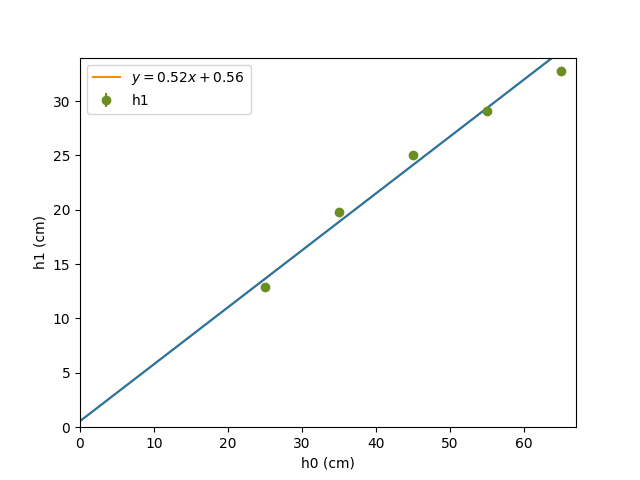
\includegraphics{Metodo1/computed_data/interpolazione_pallina3.png}
			} %close resize
		} %close centering
	\caption{Figura6: \(h1_{(h_{0})}\) - pallina da tennis - interpolazione}
	\end{figure}

	\noindent Stima del coefficiente di restituzione e della sua incertezza
	
	\[ev = \sqrt{\frac{h_{1}}{h_{0}}} \rightarrow ev = \sqrt{B}\]

	\makebox[\textwidth]{
		{	
			\normalsize
			propagazione degli errori \(\rightarrow \quad  \sigma _{ev} = \frac{\sigma _{B}}{2\sqrt{B}} \)
		}
	}
	\[ev = 0.724 \pm 0.003\]
\noindent Test del chi quadro\\
\[\chi ^{2} = \sum \left ( \frac{y_{i}-A-BX_{i}}{\sigma_{i}} \right )^{2} = 27.8\]
\noindent considerando 3 gradi di libertà \(\tilde{\chi}^{2} = 13.9 \rightarrow \) probabilità inferiore al 0.05\(\%\) che le misure abbiano seguito la distribuzione lineare assunta.\\\\
Considerando \(h_{lim} = 50 cm\), la massa della pallina come 0.056Kg ed il diametro d = 0.202 metri, il contributo dell'attrito aereo su altezze di 50cm o superiori è almeno di:
\[\frac{F_{attrito \quad aereo}}{F_{peso}} = \frac{\rho_{aria} \pi \cdot 0.4 d^{2}}{4m}h_{lim} =  0.14\]
poichè al di sopra dei 50cm la pallina da tennis viene trattenuta da una forza pari al 14 \(\%\) del suo peso, abbiamo ridotto la regione di interpolazione al di sotto dei 50 cm: i parametri della retta interpolata corretta sono
\[B =0.606 \pm 0.007\]
\[A =(-2.13 \pm 0.26) cm\]
e ci portano a stimare il coefficiente di restituzione corretto come: \(ev =  0.778 \pm 0.004\).
\[\chi ^{2}corretto = 2.28\]
nel caso con soli 3 punti possiamo considerare l'ipotesi vera, con una sicurezza del 14 \(\%\).\\
	%metodo due pallina 3
	\subsubsection*{metodo 2}

	Intervalli misurati da 65cm in secondi:
	\begin{figure}[!h]
		\makebox[1 \textwidth][c]{
			\begin{tabular}{c|*{7}{c}}
				numero rimbalzo & lancio1 & lancio2 & lancio3 & lancio4 & lancio5 & media\\
				\hline
				1 & 0.547 & 0.510 & 0.535 & 0.535 & 0.533 & \(	0.5319\pm 0.006\)\\
				\hline
				2 & 0.412 & 0.383 & 0.402 & 0.398 & 0.404 &\( 0.3996 \pm0.005\) \\
				\hline
				3 & 0.314 & 0.306 & 0.315 & 0.303 & 0.306 & \( 0.3087\pm0.0024\)\\
				\hline
				4 & 0.245 & 0.225 & 0.231 & 0.242 & 0.234 & \(0.235\pm0.004\)\\
				
				\hline
			\end{tabular}
		} 
	\end{figure}

	\noindent Intervalli misurati da 55cm in secondi:
	\begin{figure}[!h]
		\makebox[1 \textwidth][c]{
			\begin{tabular}{c|*{7}{c}}
				numero rimbalzo & lancio1 & lancio2 & lancio3 & lancio4 & lancio5 & media\\
				\hline
				1 & 0.496 & 0.505 & 0.504 & 0.500 & 0.499 & \(0.5007\pm0.0016\)\\
				\hline
				2 & 0.384 & 0.386 & 0.375 & 0.375 & 0.382 & \( 0.3805\pm0.0023\)\\
				\hline
				3 & 0.290 & 0.293 & 0.284 & 0.293 & 0.286 &\( 0.2894\pm0.0018 \) \\
				\hline
				4 & 0.230 & 0.233 & 0.226 & 0.235 & 0.228 & \( 0.2303\pm0.0017\) \\
				
				\hline
			\end{tabular}
		} 
	\end{figure}

	\noindent Intervalli misurati da 45cm in secondi:
	
	\begin{figure}[!h]
		\makebox[1 \textwidth][c]{
			\begin{tabular}{c|*{7}{c}}
				numero rimbalzo & lancio1 & lancio2 & lancio3 & lancio4 & lancio5 & media\\
				\hline
				1 & 0.453 & 0.459 & 0.456 & 0.458 & 0.458 &\(0.4567\pm 0.0010 \) \\
				\hline
				2 & 0.354 & 0.343 & 0.351 & 0.345 & 0.348 & \( 0.3483 \pm0.0021 \)\\
				\hline
				3 & 0.263 & 0.256 & 0.264 & 0.276 & 0.270 &\(	0.266\pm0.003 \) \\
				\hline
				4 & 0.199 & 0.206 & 0.212 & 0.190 & 0.210 &\( 0.203 \pm0.004\) \\
				
				\hline
			\end{tabular}
		} 
	\end{figure}

\noindent Intervalli misurati da 35cm in secondi:
	\begin{figure}[!h]
		\makebox[1 \textwidth][c]{
			\begin{tabular}{c|*{7}{c}}
				numero rimbalzo & lancio1 & lancio2 & lancio3 & lancio4 & lancio5 & media\\
				\hline
				1 & 0.411 & 0.407 & 0.408 & 0.410 & 0.407 & \(0.4087\pm0.0009 \)\\
				\hline
				2 & 0.305 & 0.309 & 0.308 & 0.311 & 0.311 &\(0.3090 \pm 0.0011\) \\
				\hline
				3 & 0.242 & 0.240 & 0.235 & 0.236 & 0.240 &\(  0.2386\pm 0.0012\) \\
				\hline
				4 & 0.178 & 0.183 & 0.177 & 0.177 & 0.186 & \( 0.1802 \pm 0.0017\)\\
				\hline
			\end{tabular}
		} 
	\end{figure}

\noindent Intervalli misurati da 25cm in secondi:
	\begin{figure}[!h]
		\makebox[1 \textwidth][c]{
			\begin{tabular}{c|*{7}{c}}
				numero rimbalzo & lancio1 & lancio2 & lancio3 & lancio4 & lancio5 & media\\
				\hline
				1 & 0.350 & 0.349 & 0.352 & 0.347 & 0.355 & \(0.3505\pm0.0013\)\\
				\hline
				2 & 0.267 & 0.268 & 0.271 & 0.268 & 0.272 & \( 0.2692 \pm 0.0010\)\\
				\hline
				3 & 0.203 & 0.215 & 0.209 & 0.203 & 0.206 &\(  0.2073 \pm0.0023 \) \\
				\hline
				4 & 0.153 & 0.144 & 0.146 & 0.150 & 0.160 &\( 0.1508\pm0.0027\) \\
				\hline
			\end{tabular}
		} 
	\end{figure}
	
.\\\\\\\\\\\\
	\begin{figure}[!ht]
				\captionsetup{labelformat=empty}
		\makebox[1 \textwidth][c]{       %centering table
			\resizebox{0.7 \textwidth}{!}{   %resize table
				%%% Creator: Matplotlib, PGF backend
%%
%% To include the figure in your LaTeX document, write
%%   \input{<filename>.pgf}
%%
%% Make sure the required packages are loaded in your preamble
%%   \usepackage{pgf}
%%
%% and, on pdftex
%%   \usepackage[utf8]{inputenc}\DeclareUnicodeCharacter{2212}{-}
%%
%% or, on luatex and xetex
%%   \usepackage{unicode-math}
%%
%% Figures using additional raster images can only be included by \input if
%% they are in the same directory as the main LaTeX file. For loading figures
%% from other directories you can use the `import` package
%%   \usepackage{import}
%%
%% and then include the figures with
%%   \import{<path to file>}{<filename>.pgf}
%%
%% Matplotlib used the following preamble
%%   \usepackage{fontspec}
%%   \setmainfont{DejaVuSerif.ttf}[Path=C:/Users/giuly/AppData/Local/Programs/Python/Python39/Lib/site-packages/matplotlib/mpl-data/fonts/ttf/]
%%   \setsansfont{DejaVuSans.ttf}[Path=C:/Users/giuly/AppData/Local/Programs/Python/Python39/Lib/site-packages/matplotlib/mpl-data/fonts/ttf/]
%%   \setmonofont{DejaVuSansMono.ttf}[Path=C:/Users/giuly/AppData/Local/Programs/Python/Python39/Lib/site-packages/matplotlib/mpl-data/fonts/ttf/]
%%
\begingroup%
\makeatletter%
\begin{pgfpicture}%
\pgfpathrectangle{\pgfpointorigin}{\pgfqpoint{6.400000in}{4.800000in}}%
\pgfusepath{use as bounding box, clip}%
\begin{pgfscope}%
\pgfsetbuttcap%
\pgfsetmiterjoin%
\definecolor{currentfill}{rgb}{1.000000,1.000000,1.000000}%
\pgfsetfillcolor{currentfill}%
\pgfsetlinewidth{0.000000pt}%
\definecolor{currentstroke}{rgb}{1.000000,1.000000,1.000000}%
\pgfsetstrokecolor{currentstroke}%
\pgfsetdash{}{0pt}%
\pgfpathmoveto{\pgfqpoint{0.000000in}{0.000000in}}%
\pgfpathlineto{\pgfqpoint{6.400000in}{0.000000in}}%
\pgfpathlineto{\pgfqpoint{6.400000in}{4.800000in}}%
\pgfpathlineto{\pgfqpoint{0.000000in}{4.800000in}}%
\pgfpathclose%
\pgfusepath{fill}%
\end{pgfscope}%
\begin{pgfscope}%
\pgfsetbuttcap%
\pgfsetmiterjoin%
\definecolor{currentfill}{rgb}{1.000000,1.000000,1.000000}%
\pgfsetfillcolor{currentfill}%
\pgfsetlinewidth{0.000000pt}%
\definecolor{currentstroke}{rgb}{0.000000,0.000000,0.000000}%
\pgfsetstrokecolor{currentstroke}%
\pgfsetstrokeopacity{0.000000}%
\pgfsetdash{}{0pt}%
\pgfpathmoveto{\pgfqpoint{0.800000in}{0.528000in}}%
\pgfpathlineto{\pgfqpoint{5.760000in}{0.528000in}}%
\pgfpathlineto{\pgfqpoint{5.760000in}{4.224000in}}%
\pgfpathlineto{\pgfqpoint{0.800000in}{4.224000in}}%
\pgfpathclose%
\pgfusepath{fill}%
\end{pgfscope}%
\begin{pgfscope}%
\pgfpathrectangle{\pgfqpoint{0.800000in}{0.528000in}}{\pgfqpoint{4.960000in}{3.696000in}}%
\pgfusepath{clip}%
\pgfsetbuttcap%
\pgfsetmiterjoin%
\definecolor{currentfill}{rgb}{0.400000,0.803922,0.666667}%
\pgfsetfillcolor{currentfill}%
\pgfsetfillopacity{0.800000}%
\pgfsetlinewidth{0.000000pt}%
\definecolor{currentstroke}{rgb}{0.000000,0.000000,0.000000}%
\pgfsetstrokecolor{currentstroke}%
\pgfsetstrokeopacity{0.800000}%
\pgfsetdash{}{0pt}%
\pgfpathmoveto{\pgfqpoint{1.025455in}{0.528000in}}%
\pgfpathlineto{\pgfqpoint{1.401212in}{0.528000in}}%
\pgfpathlineto{\pgfqpoint{1.401212in}{0.848000in}}%
\pgfpathlineto{\pgfqpoint{1.025455in}{0.848000in}}%
\pgfpathclose%
\pgfusepath{fill}%
\end{pgfscope}%
\begin{pgfscope}%
\pgfpathrectangle{\pgfqpoint{0.800000in}{0.528000in}}{\pgfqpoint{4.960000in}{3.696000in}}%
\pgfusepath{clip}%
\pgfsetbuttcap%
\pgfsetmiterjoin%
\definecolor{currentfill}{rgb}{0.400000,0.803922,0.666667}%
\pgfsetfillcolor{currentfill}%
\pgfsetfillopacity{0.800000}%
\pgfsetlinewidth{0.000000pt}%
\definecolor{currentstroke}{rgb}{0.000000,0.000000,0.000000}%
\pgfsetstrokecolor{currentstroke}%
\pgfsetstrokeopacity{0.800000}%
\pgfsetdash{}{0pt}%
\pgfpathmoveto{\pgfqpoint{1.401212in}{0.528000in}}%
\pgfpathlineto{\pgfqpoint{1.776970in}{0.528000in}}%
\pgfpathlineto{\pgfqpoint{1.776970in}{0.848000in}}%
\pgfpathlineto{\pgfqpoint{1.401212in}{0.848000in}}%
\pgfpathclose%
\pgfusepath{fill}%
\end{pgfscope}%
\begin{pgfscope}%
\pgfpathrectangle{\pgfqpoint{0.800000in}{0.528000in}}{\pgfqpoint{4.960000in}{3.696000in}}%
\pgfusepath{clip}%
\pgfsetbuttcap%
\pgfsetmiterjoin%
\definecolor{currentfill}{rgb}{0.400000,0.803922,0.666667}%
\pgfsetfillcolor{currentfill}%
\pgfsetfillopacity{0.800000}%
\pgfsetlinewidth{0.000000pt}%
\definecolor{currentstroke}{rgb}{0.000000,0.000000,0.000000}%
\pgfsetstrokecolor{currentstroke}%
\pgfsetstrokeopacity{0.800000}%
\pgfsetdash{}{0pt}%
\pgfpathmoveto{\pgfqpoint{1.776970in}{0.528000in}}%
\pgfpathlineto{\pgfqpoint{2.152727in}{0.528000in}}%
\pgfpathlineto{\pgfqpoint{2.152727in}{1.168000in}}%
\pgfpathlineto{\pgfqpoint{1.776970in}{1.168000in}}%
\pgfpathclose%
\pgfusepath{fill}%
\end{pgfscope}%
\begin{pgfscope}%
\pgfpathrectangle{\pgfqpoint{0.800000in}{0.528000in}}{\pgfqpoint{4.960000in}{3.696000in}}%
\pgfusepath{clip}%
\pgfsetbuttcap%
\pgfsetmiterjoin%
\definecolor{currentfill}{rgb}{0.400000,0.803922,0.666667}%
\pgfsetfillcolor{currentfill}%
\pgfsetfillopacity{0.800000}%
\pgfsetlinewidth{0.000000pt}%
\definecolor{currentstroke}{rgb}{0.000000,0.000000,0.000000}%
\pgfsetstrokecolor{currentstroke}%
\pgfsetstrokeopacity{0.800000}%
\pgfsetdash{}{0pt}%
\pgfpathmoveto{\pgfqpoint{2.152727in}{0.528000in}}%
\pgfpathlineto{\pgfqpoint{2.528485in}{0.528000in}}%
\pgfpathlineto{\pgfqpoint{2.528485in}{1.968000in}}%
\pgfpathlineto{\pgfqpoint{2.152727in}{1.968000in}}%
\pgfpathclose%
\pgfusepath{fill}%
\end{pgfscope}%
\begin{pgfscope}%
\pgfpathrectangle{\pgfqpoint{0.800000in}{0.528000in}}{\pgfqpoint{4.960000in}{3.696000in}}%
\pgfusepath{clip}%
\pgfsetbuttcap%
\pgfsetmiterjoin%
\definecolor{currentfill}{rgb}{0.400000,0.803922,0.666667}%
\pgfsetfillcolor{currentfill}%
\pgfsetfillopacity{0.800000}%
\pgfsetlinewidth{0.000000pt}%
\definecolor{currentstroke}{rgb}{0.000000,0.000000,0.000000}%
\pgfsetstrokecolor{currentstroke}%
\pgfsetstrokeopacity{0.800000}%
\pgfsetdash{}{0pt}%
\pgfpathmoveto{\pgfqpoint{2.528485in}{0.528000in}}%
\pgfpathlineto{\pgfqpoint{2.904242in}{0.528000in}}%
\pgfpathlineto{\pgfqpoint{2.904242in}{2.448000in}}%
\pgfpathlineto{\pgfqpoint{2.528485in}{2.448000in}}%
\pgfpathclose%
\pgfusepath{fill}%
\end{pgfscope}%
\begin{pgfscope}%
\pgfpathrectangle{\pgfqpoint{0.800000in}{0.528000in}}{\pgfqpoint{4.960000in}{3.696000in}}%
\pgfusepath{clip}%
\pgfsetbuttcap%
\pgfsetmiterjoin%
\definecolor{currentfill}{rgb}{0.400000,0.803922,0.666667}%
\pgfsetfillcolor{currentfill}%
\pgfsetfillopacity{0.800000}%
\pgfsetlinewidth{0.000000pt}%
\definecolor{currentstroke}{rgb}{0.000000,0.000000,0.000000}%
\pgfsetstrokecolor{currentstroke}%
\pgfsetstrokeopacity{0.800000}%
\pgfsetdash{}{0pt}%
\pgfpathmoveto{\pgfqpoint{2.904242in}{0.528000in}}%
\pgfpathlineto{\pgfqpoint{3.280000in}{0.528000in}}%
\pgfpathlineto{\pgfqpoint{3.280000in}{4.048000in}}%
\pgfpathlineto{\pgfqpoint{2.904242in}{4.048000in}}%
\pgfpathclose%
\pgfusepath{fill}%
\end{pgfscope}%
\begin{pgfscope}%
\pgfpathrectangle{\pgfqpoint{0.800000in}{0.528000in}}{\pgfqpoint{4.960000in}{3.696000in}}%
\pgfusepath{clip}%
\pgfsetbuttcap%
\pgfsetmiterjoin%
\definecolor{currentfill}{rgb}{0.400000,0.803922,0.666667}%
\pgfsetfillcolor{currentfill}%
\pgfsetfillopacity{0.800000}%
\pgfsetlinewidth{0.000000pt}%
\definecolor{currentstroke}{rgb}{0.000000,0.000000,0.000000}%
\pgfsetstrokecolor{currentstroke}%
\pgfsetstrokeopacity{0.800000}%
\pgfsetdash{}{0pt}%
\pgfpathmoveto{\pgfqpoint{3.280000in}{0.528000in}}%
\pgfpathlineto{\pgfqpoint{3.655758in}{0.528000in}}%
\pgfpathlineto{\pgfqpoint{3.655758in}{3.248000in}}%
\pgfpathlineto{\pgfqpoint{3.280000in}{3.248000in}}%
\pgfpathclose%
\pgfusepath{fill}%
\end{pgfscope}%
\begin{pgfscope}%
\pgfpathrectangle{\pgfqpoint{0.800000in}{0.528000in}}{\pgfqpoint{4.960000in}{3.696000in}}%
\pgfusepath{clip}%
\pgfsetbuttcap%
\pgfsetmiterjoin%
\definecolor{currentfill}{rgb}{0.400000,0.803922,0.666667}%
\pgfsetfillcolor{currentfill}%
\pgfsetfillopacity{0.800000}%
\pgfsetlinewidth{0.000000pt}%
\definecolor{currentstroke}{rgb}{0.000000,0.000000,0.000000}%
\pgfsetstrokecolor{currentstroke}%
\pgfsetstrokeopacity{0.800000}%
\pgfsetdash{}{0pt}%
\pgfpathmoveto{\pgfqpoint{3.655758in}{0.528000in}}%
\pgfpathlineto{\pgfqpoint{4.031515in}{0.528000in}}%
\pgfpathlineto{\pgfqpoint{4.031515in}{3.248000in}}%
\pgfpathlineto{\pgfqpoint{3.655758in}{3.248000in}}%
\pgfpathclose%
\pgfusepath{fill}%
\end{pgfscope}%
\begin{pgfscope}%
\pgfpathrectangle{\pgfqpoint{0.800000in}{0.528000in}}{\pgfqpoint{4.960000in}{3.696000in}}%
\pgfusepath{clip}%
\pgfsetbuttcap%
\pgfsetmiterjoin%
\definecolor{currentfill}{rgb}{0.400000,0.803922,0.666667}%
\pgfsetfillcolor{currentfill}%
\pgfsetfillopacity{0.800000}%
\pgfsetlinewidth{0.000000pt}%
\definecolor{currentstroke}{rgb}{0.000000,0.000000,0.000000}%
\pgfsetstrokecolor{currentstroke}%
\pgfsetstrokeopacity{0.800000}%
\pgfsetdash{}{0pt}%
\pgfpathmoveto{\pgfqpoint{4.031515in}{0.528000in}}%
\pgfpathlineto{\pgfqpoint{4.407273in}{0.528000in}}%
\pgfpathlineto{\pgfqpoint{4.407273in}{1.968000in}}%
\pgfpathlineto{\pgfqpoint{4.031515in}{1.968000in}}%
\pgfpathclose%
\pgfusepath{fill}%
\end{pgfscope}%
\begin{pgfscope}%
\pgfpathrectangle{\pgfqpoint{0.800000in}{0.528000in}}{\pgfqpoint{4.960000in}{3.696000in}}%
\pgfusepath{clip}%
\pgfsetbuttcap%
\pgfsetmiterjoin%
\definecolor{currentfill}{rgb}{0.400000,0.803922,0.666667}%
\pgfsetfillcolor{currentfill}%
\pgfsetfillopacity{0.800000}%
\pgfsetlinewidth{0.000000pt}%
\definecolor{currentstroke}{rgb}{0.000000,0.000000,0.000000}%
\pgfsetstrokecolor{currentstroke}%
\pgfsetstrokeopacity{0.800000}%
\pgfsetdash{}{0pt}%
\pgfpathmoveto{\pgfqpoint{4.407273in}{0.528000in}}%
\pgfpathlineto{\pgfqpoint{4.783030in}{0.528000in}}%
\pgfpathlineto{\pgfqpoint{4.783030in}{1.168000in}}%
\pgfpathlineto{\pgfqpoint{4.407273in}{1.168000in}}%
\pgfpathclose%
\pgfusepath{fill}%
\end{pgfscope}%
\begin{pgfscope}%
\pgfpathrectangle{\pgfqpoint{0.800000in}{0.528000in}}{\pgfqpoint{4.960000in}{3.696000in}}%
\pgfusepath{clip}%
\pgfsetbuttcap%
\pgfsetmiterjoin%
\definecolor{currentfill}{rgb}{0.400000,0.803922,0.666667}%
\pgfsetfillcolor{currentfill}%
\pgfsetfillopacity{0.800000}%
\pgfsetlinewidth{0.000000pt}%
\definecolor{currentstroke}{rgb}{0.000000,0.000000,0.000000}%
\pgfsetstrokecolor{currentstroke}%
\pgfsetstrokeopacity{0.800000}%
\pgfsetdash{}{0pt}%
\pgfpathmoveto{\pgfqpoint{4.783030in}{0.528000in}}%
\pgfpathlineto{\pgfqpoint{5.158788in}{0.528000in}}%
\pgfpathlineto{\pgfqpoint{5.158788in}{0.688000in}}%
\pgfpathlineto{\pgfqpoint{4.783030in}{0.688000in}}%
\pgfpathclose%
\pgfusepath{fill}%
\end{pgfscope}%
\begin{pgfscope}%
\pgfpathrectangle{\pgfqpoint{0.800000in}{0.528000in}}{\pgfqpoint{4.960000in}{3.696000in}}%
\pgfusepath{clip}%
\pgfsetbuttcap%
\pgfsetmiterjoin%
\definecolor{currentfill}{rgb}{0.400000,0.803922,0.666667}%
\pgfsetfillcolor{currentfill}%
\pgfsetfillopacity{0.800000}%
\pgfsetlinewidth{0.000000pt}%
\definecolor{currentstroke}{rgb}{0.000000,0.000000,0.000000}%
\pgfsetstrokecolor{currentstroke}%
\pgfsetstrokeopacity{0.800000}%
\pgfsetdash{}{0pt}%
\pgfpathmoveto{\pgfqpoint{5.158788in}{0.528000in}}%
\pgfpathlineto{\pgfqpoint{5.534545in}{0.528000in}}%
\pgfpathlineto{\pgfqpoint{5.534545in}{0.688000in}}%
\pgfpathlineto{\pgfqpoint{5.158788in}{0.688000in}}%
\pgfpathclose%
\pgfusepath{fill}%
\end{pgfscope}%
\begin{pgfscope}%
\pgfsetbuttcap%
\pgfsetroundjoin%
\definecolor{currentfill}{rgb}{0.000000,0.000000,0.000000}%
\pgfsetfillcolor{currentfill}%
\pgfsetlinewidth{0.803000pt}%
\definecolor{currentstroke}{rgb}{0.000000,0.000000,0.000000}%
\pgfsetstrokecolor{currentstroke}%
\pgfsetdash{}{0pt}%
\pgfsys@defobject{currentmarker}{\pgfqpoint{0.000000in}{-0.048611in}}{\pgfqpoint{0.000000in}{0.000000in}}{%
\pgfpathmoveto{\pgfqpoint{0.000000in}{0.000000in}}%
\pgfpathlineto{\pgfqpoint{0.000000in}{-0.048611in}}%
\pgfusepath{stroke,fill}%
}%
\begin{pgfscope}%
\pgfsys@transformshift{1.025455in}{0.528000in}%
\pgfsys@useobject{currentmarker}{}%
\end{pgfscope}%
\end{pgfscope}%
\begin{pgfscope}%
\definecolor{textcolor}{rgb}{0.000000,0.000000,0.000000}%
\pgfsetstrokecolor{textcolor}%
\pgfsetfillcolor{textcolor}%
\pgftext[x=1.025455in,y=0.430778in,,top]{\color{textcolor}\sffamily\fontsize{10.000000}{12.000000}\selectfont 1.30}%
\end{pgfscope}%
\begin{pgfscope}%
\pgfsetbuttcap%
\pgfsetroundjoin%
\definecolor{currentfill}{rgb}{0.000000,0.000000,0.000000}%
\pgfsetfillcolor{currentfill}%
\pgfsetlinewidth{0.803000pt}%
\definecolor{currentstroke}{rgb}{0.000000,0.000000,0.000000}%
\pgfsetstrokecolor{currentstroke}%
\pgfsetdash{}{0pt}%
\pgfsys@defobject{currentmarker}{\pgfqpoint{0.000000in}{-0.048611in}}{\pgfqpoint{0.000000in}{0.000000in}}{%
\pgfpathmoveto{\pgfqpoint{0.000000in}{0.000000in}}%
\pgfpathlineto{\pgfqpoint{0.000000in}{-0.048611in}}%
\pgfusepath{stroke,fill}%
}%
\begin{pgfscope}%
\pgfsys@transformshift{1.589091in}{0.528000in}%
\pgfsys@useobject{currentmarker}{}%
\end{pgfscope}%
\end{pgfscope}%
\begin{pgfscope}%
\definecolor{textcolor}{rgb}{0.000000,0.000000,0.000000}%
\pgfsetstrokecolor{textcolor}%
\pgfsetfillcolor{textcolor}%
\pgftext[x=1.589091in,y=0.430778in,,top]{\color{textcolor}\sffamily\fontsize{10.000000}{12.000000}\selectfont 1.35}%
\end{pgfscope}%
\begin{pgfscope}%
\pgfsetbuttcap%
\pgfsetroundjoin%
\definecolor{currentfill}{rgb}{0.000000,0.000000,0.000000}%
\pgfsetfillcolor{currentfill}%
\pgfsetlinewidth{0.803000pt}%
\definecolor{currentstroke}{rgb}{0.000000,0.000000,0.000000}%
\pgfsetstrokecolor{currentstroke}%
\pgfsetdash{}{0pt}%
\pgfsys@defobject{currentmarker}{\pgfqpoint{0.000000in}{-0.048611in}}{\pgfqpoint{0.000000in}{0.000000in}}{%
\pgfpathmoveto{\pgfqpoint{0.000000in}{0.000000in}}%
\pgfpathlineto{\pgfqpoint{0.000000in}{-0.048611in}}%
\pgfusepath{stroke,fill}%
}%
\begin{pgfscope}%
\pgfsys@transformshift{2.152727in}{0.528000in}%
\pgfsys@useobject{currentmarker}{}%
\end{pgfscope}%
\end{pgfscope}%
\begin{pgfscope}%
\definecolor{textcolor}{rgb}{0.000000,0.000000,0.000000}%
\pgfsetstrokecolor{textcolor}%
\pgfsetfillcolor{textcolor}%
\pgftext[x=2.152727in,y=0.430778in,,top]{\color{textcolor}\sffamily\fontsize{10.000000}{12.000000}\selectfont 1.40}%
\end{pgfscope}%
\begin{pgfscope}%
\pgfsetbuttcap%
\pgfsetroundjoin%
\definecolor{currentfill}{rgb}{0.000000,0.000000,0.000000}%
\pgfsetfillcolor{currentfill}%
\pgfsetlinewidth{0.803000pt}%
\definecolor{currentstroke}{rgb}{0.000000,0.000000,0.000000}%
\pgfsetstrokecolor{currentstroke}%
\pgfsetdash{}{0pt}%
\pgfsys@defobject{currentmarker}{\pgfqpoint{0.000000in}{-0.048611in}}{\pgfqpoint{0.000000in}{0.000000in}}{%
\pgfpathmoveto{\pgfqpoint{0.000000in}{0.000000in}}%
\pgfpathlineto{\pgfqpoint{0.000000in}{-0.048611in}}%
\pgfusepath{stroke,fill}%
}%
\begin{pgfscope}%
\pgfsys@transformshift{2.716364in}{0.528000in}%
\pgfsys@useobject{currentmarker}{}%
\end{pgfscope}%
\end{pgfscope}%
\begin{pgfscope}%
\definecolor{textcolor}{rgb}{0.000000,0.000000,0.000000}%
\pgfsetstrokecolor{textcolor}%
\pgfsetfillcolor{textcolor}%
\pgftext[x=2.716364in,y=0.430778in,,top]{\color{textcolor}\sffamily\fontsize{10.000000}{12.000000}\selectfont 1.45}%
\end{pgfscope}%
\begin{pgfscope}%
\pgfsetbuttcap%
\pgfsetroundjoin%
\definecolor{currentfill}{rgb}{0.000000,0.000000,0.000000}%
\pgfsetfillcolor{currentfill}%
\pgfsetlinewidth{0.803000pt}%
\definecolor{currentstroke}{rgb}{0.000000,0.000000,0.000000}%
\pgfsetstrokecolor{currentstroke}%
\pgfsetdash{}{0pt}%
\pgfsys@defobject{currentmarker}{\pgfqpoint{0.000000in}{-0.048611in}}{\pgfqpoint{0.000000in}{0.000000in}}{%
\pgfpathmoveto{\pgfqpoint{0.000000in}{0.000000in}}%
\pgfpathlineto{\pgfqpoint{0.000000in}{-0.048611in}}%
\pgfusepath{stroke,fill}%
}%
\begin{pgfscope}%
\pgfsys@transformshift{3.280000in}{0.528000in}%
\pgfsys@useobject{currentmarker}{}%
\end{pgfscope}%
\end{pgfscope}%
\begin{pgfscope}%
\definecolor{textcolor}{rgb}{0.000000,0.000000,0.000000}%
\pgfsetstrokecolor{textcolor}%
\pgfsetfillcolor{textcolor}%
\pgftext[x=3.280000in,y=0.430778in,,top]{\color{textcolor}\sffamily\fontsize{10.000000}{12.000000}\selectfont 1.50}%
\end{pgfscope}%
\begin{pgfscope}%
\pgfsetbuttcap%
\pgfsetroundjoin%
\definecolor{currentfill}{rgb}{0.000000,0.000000,0.000000}%
\pgfsetfillcolor{currentfill}%
\pgfsetlinewidth{0.803000pt}%
\definecolor{currentstroke}{rgb}{0.000000,0.000000,0.000000}%
\pgfsetstrokecolor{currentstroke}%
\pgfsetdash{}{0pt}%
\pgfsys@defobject{currentmarker}{\pgfqpoint{0.000000in}{-0.048611in}}{\pgfqpoint{0.000000in}{0.000000in}}{%
\pgfpathmoveto{\pgfqpoint{0.000000in}{0.000000in}}%
\pgfpathlineto{\pgfqpoint{0.000000in}{-0.048611in}}%
\pgfusepath{stroke,fill}%
}%
\begin{pgfscope}%
\pgfsys@transformshift{3.843636in}{0.528000in}%
\pgfsys@useobject{currentmarker}{}%
\end{pgfscope}%
\end{pgfscope}%
\begin{pgfscope}%
\definecolor{textcolor}{rgb}{0.000000,0.000000,0.000000}%
\pgfsetstrokecolor{textcolor}%
\pgfsetfillcolor{textcolor}%
\pgftext[x=3.843636in,y=0.430778in,,top]{\color{textcolor}\sffamily\fontsize{10.000000}{12.000000}\selectfont 1.55}%
\end{pgfscope}%
\begin{pgfscope}%
\pgfsetbuttcap%
\pgfsetroundjoin%
\definecolor{currentfill}{rgb}{0.000000,0.000000,0.000000}%
\pgfsetfillcolor{currentfill}%
\pgfsetlinewidth{0.803000pt}%
\definecolor{currentstroke}{rgb}{0.000000,0.000000,0.000000}%
\pgfsetstrokecolor{currentstroke}%
\pgfsetdash{}{0pt}%
\pgfsys@defobject{currentmarker}{\pgfqpoint{0.000000in}{-0.048611in}}{\pgfqpoint{0.000000in}{0.000000in}}{%
\pgfpathmoveto{\pgfqpoint{0.000000in}{0.000000in}}%
\pgfpathlineto{\pgfqpoint{0.000000in}{-0.048611in}}%
\pgfusepath{stroke,fill}%
}%
\begin{pgfscope}%
\pgfsys@transformshift{4.407273in}{0.528000in}%
\pgfsys@useobject{currentmarker}{}%
\end{pgfscope}%
\end{pgfscope}%
\begin{pgfscope}%
\definecolor{textcolor}{rgb}{0.000000,0.000000,0.000000}%
\pgfsetstrokecolor{textcolor}%
\pgfsetfillcolor{textcolor}%
\pgftext[x=4.407273in,y=0.430778in,,top]{\color{textcolor}\sffamily\fontsize{10.000000}{12.000000}\selectfont 1.60}%
\end{pgfscope}%
\begin{pgfscope}%
\pgfsetbuttcap%
\pgfsetroundjoin%
\definecolor{currentfill}{rgb}{0.000000,0.000000,0.000000}%
\pgfsetfillcolor{currentfill}%
\pgfsetlinewidth{0.803000pt}%
\definecolor{currentstroke}{rgb}{0.000000,0.000000,0.000000}%
\pgfsetstrokecolor{currentstroke}%
\pgfsetdash{}{0pt}%
\pgfsys@defobject{currentmarker}{\pgfqpoint{0.000000in}{-0.048611in}}{\pgfqpoint{0.000000in}{0.000000in}}{%
\pgfpathmoveto{\pgfqpoint{0.000000in}{0.000000in}}%
\pgfpathlineto{\pgfqpoint{0.000000in}{-0.048611in}}%
\pgfusepath{stroke,fill}%
}%
\begin{pgfscope}%
\pgfsys@transformshift{4.970909in}{0.528000in}%
\pgfsys@useobject{currentmarker}{}%
\end{pgfscope}%
\end{pgfscope}%
\begin{pgfscope}%
\definecolor{textcolor}{rgb}{0.000000,0.000000,0.000000}%
\pgfsetstrokecolor{textcolor}%
\pgfsetfillcolor{textcolor}%
\pgftext[x=4.970909in,y=0.430778in,,top]{\color{textcolor}\sffamily\fontsize{10.000000}{12.000000}\selectfont 1.65}%
\end{pgfscope}%
\begin{pgfscope}%
\pgfsetbuttcap%
\pgfsetroundjoin%
\definecolor{currentfill}{rgb}{0.000000,0.000000,0.000000}%
\pgfsetfillcolor{currentfill}%
\pgfsetlinewidth{0.803000pt}%
\definecolor{currentstroke}{rgb}{0.000000,0.000000,0.000000}%
\pgfsetstrokecolor{currentstroke}%
\pgfsetdash{}{0pt}%
\pgfsys@defobject{currentmarker}{\pgfqpoint{0.000000in}{-0.048611in}}{\pgfqpoint{0.000000in}{0.000000in}}{%
\pgfpathmoveto{\pgfqpoint{0.000000in}{0.000000in}}%
\pgfpathlineto{\pgfqpoint{0.000000in}{-0.048611in}}%
\pgfusepath{stroke,fill}%
}%
\begin{pgfscope}%
\pgfsys@transformshift{5.534545in}{0.528000in}%
\pgfsys@useobject{currentmarker}{}%
\end{pgfscope}%
\end{pgfscope}%
\begin{pgfscope}%
\definecolor{textcolor}{rgb}{0.000000,0.000000,0.000000}%
\pgfsetstrokecolor{textcolor}%
\pgfsetfillcolor{textcolor}%
\pgftext[x=5.534545in,y=0.430778in,,top]{\color{textcolor}\sffamily\fontsize{10.000000}{12.000000}\selectfont 1.70}%
\end{pgfscope}%
\begin{pgfscope}%
\definecolor{textcolor}{rgb}{0.000000,0.000000,0.000000}%
\pgfsetstrokecolor{textcolor}%
\pgfsetfillcolor{textcolor}%
\pgftext[x=3.280000in,y=0.240809in,,top]{\color{textcolor}\sffamily\fontsize{10.000000}{12.000000}\selectfont \(\displaystyle x_k\) (s)}%
\end{pgfscope}%
\begin{pgfscope}%
\pgfsetbuttcap%
\pgfsetroundjoin%
\definecolor{currentfill}{rgb}{0.000000,0.000000,0.000000}%
\pgfsetfillcolor{currentfill}%
\pgfsetlinewidth{0.803000pt}%
\definecolor{currentstroke}{rgb}{0.000000,0.000000,0.000000}%
\pgfsetstrokecolor{currentstroke}%
\pgfsetdash{}{0pt}%
\pgfsys@defobject{currentmarker}{\pgfqpoint{-0.048611in}{0.000000in}}{\pgfqpoint{-0.000000in}{0.000000in}}{%
\pgfpathmoveto{\pgfqpoint{-0.000000in}{0.000000in}}%
\pgfpathlineto{\pgfqpoint{-0.048611in}{0.000000in}}%
\pgfusepath{stroke,fill}%
}%
\begin{pgfscope}%
\pgfsys@transformshift{0.800000in}{0.528000in}%
\pgfsys@useobject{currentmarker}{}%
\end{pgfscope}%
\end{pgfscope}%
\begin{pgfscope}%
\definecolor{textcolor}{rgb}{0.000000,0.000000,0.000000}%
\pgfsetstrokecolor{textcolor}%
\pgfsetfillcolor{textcolor}%
\pgftext[x=0.614412in, y=0.475238in, left, base]{\color{textcolor}\sffamily\fontsize{10.000000}{12.000000}\selectfont 0}%
\end{pgfscope}%
\begin{pgfscope}%
\pgfsetbuttcap%
\pgfsetroundjoin%
\definecolor{currentfill}{rgb}{0.000000,0.000000,0.000000}%
\pgfsetfillcolor{currentfill}%
\pgfsetlinewidth{0.803000pt}%
\definecolor{currentstroke}{rgb}{0.000000,0.000000,0.000000}%
\pgfsetstrokecolor{currentstroke}%
\pgfsetdash{}{0pt}%
\pgfsys@defobject{currentmarker}{\pgfqpoint{-0.048611in}{0.000000in}}{\pgfqpoint{-0.000000in}{0.000000in}}{%
\pgfpathmoveto{\pgfqpoint{-0.000000in}{0.000000in}}%
\pgfpathlineto{\pgfqpoint{-0.048611in}{0.000000in}}%
\pgfusepath{stroke,fill}%
}%
\begin{pgfscope}%
\pgfsys@transformshift{0.800000in}{1.061333in}%
\pgfsys@useobject{currentmarker}{}%
\end{pgfscope}%
\end{pgfscope}%
\begin{pgfscope}%
\definecolor{textcolor}{rgb}{0.000000,0.000000,0.000000}%
\pgfsetstrokecolor{textcolor}%
\pgfsetfillcolor{textcolor}%
\pgftext[x=0.614412in, y=1.008572in, left, base]{\color{textcolor}\sffamily\fontsize{10.000000}{12.000000}\selectfont 1}%
\end{pgfscope}%
\begin{pgfscope}%
\pgfsetbuttcap%
\pgfsetroundjoin%
\definecolor{currentfill}{rgb}{0.000000,0.000000,0.000000}%
\pgfsetfillcolor{currentfill}%
\pgfsetlinewidth{0.803000pt}%
\definecolor{currentstroke}{rgb}{0.000000,0.000000,0.000000}%
\pgfsetstrokecolor{currentstroke}%
\pgfsetdash{}{0pt}%
\pgfsys@defobject{currentmarker}{\pgfqpoint{-0.048611in}{0.000000in}}{\pgfqpoint{-0.000000in}{0.000000in}}{%
\pgfpathmoveto{\pgfqpoint{-0.000000in}{0.000000in}}%
\pgfpathlineto{\pgfqpoint{-0.048611in}{0.000000in}}%
\pgfusepath{stroke,fill}%
}%
\begin{pgfscope}%
\pgfsys@transformshift{0.800000in}{1.594667in}%
\pgfsys@useobject{currentmarker}{}%
\end{pgfscope}%
\end{pgfscope}%
\begin{pgfscope}%
\definecolor{textcolor}{rgb}{0.000000,0.000000,0.000000}%
\pgfsetstrokecolor{textcolor}%
\pgfsetfillcolor{textcolor}%
\pgftext[x=0.614412in, y=1.541905in, left, base]{\color{textcolor}\sffamily\fontsize{10.000000}{12.000000}\selectfont 2}%
\end{pgfscope}%
\begin{pgfscope}%
\pgfsetbuttcap%
\pgfsetroundjoin%
\definecolor{currentfill}{rgb}{0.000000,0.000000,0.000000}%
\pgfsetfillcolor{currentfill}%
\pgfsetlinewidth{0.803000pt}%
\definecolor{currentstroke}{rgb}{0.000000,0.000000,0.000000}%
\pgfsetstrokecolor{currentstroke}%
\pgfsetdash{}{0pt}%
\pgfsys@defobject{currentmarker}{\pgfqpoint{-0.048611in}{0.000000in}}{\pgfqpoint{-0.000000in}{0.000000in}}{%
\pgfpathmoveto{\pgfqpoint{-0.000000in}{0.000000in}}%
\pgfpathlineto{\pgfqpoint{-0.048611in}{0.000000in}}%
\pgfusepath{stroke,fill}%
}%
\begin{pgfscope}%
\pgfsys@transformshift{0.800000in}{2.128000in}%
\pgfsys@useobject{currentmarker}{}%
\end{pgfscope}%
\end{pgfscope}%
\begin{pgfscope}%
\definecolor{textcolor}{rgb}{0.000000,0.000000,0.000000}%
\pgfsetstrokecolor{textcolor}%
\pgfsetfillcolor{textcolor}%
\pgftext[x=0.614412in, y=2.075238in, left, base]{\color{textcolor}\sffamily\fontsize{10.000000}{12.000000}\selectfont 3}%
\end{pgfscope}%
\begin{pgfscope}%
\pgfsetbuttcap%
\pgfsetroundjoin%
\definecolor{currentfill}{rgb}{0.000000,0.000000,0.000000}%
\pgfsetfillcolor{currentfill}%
\pgfsetlinewidth{0.803000pt}%
\definecolor{currentstroke}{rgb}{0.000000,0.000000,0.000000}%
\pgfsetstrokecolor{currentstroke}%
\pgfsetdash{}{0pt}%
\pgfsys@defobject{currentmarker}{\pgfqpoint{-0.048611in}{0.000000in}}{\pgfqpoint{-0.000000in}{0.000000in}}{%
\pgfpathmoveto{\pgfqpoint{-0.000000in}{0.000000in}}%
\pgfpathlineto{\pgfqpoint{-0.048611in}{0.000000in}}%
\pgfusepath{stroke,fill}%
}%
\begin{pgfscope}%
\pgfsys@transformshift{0.800000in}{2.661333in}%
\pgfsys@useobject{currentmarker}{}%
\end{pgfscope}%
\end{pgfscope}%
\begin{pgfscope}%
\definecolor{textcolor}{rgb}{0.000000,0.000000,0.000000}%
\pgfsetstrokecolor{textcolor}%
\pgfsetfillcolor{textcolor}%
\pgftext[x=0.614412in, y=2.608572in, left, base]{\color{textcolor}\sffamily\fontsize{10.000000}{12.000000}\selectfont 4}%
\end{pgfscope}%
\begin{pgfscope}%
\pgfsetbuttcap%
\pgfsetroundjoin%
\definecolor{currentfill}{rgb}{0.000000,0.000000,0.000000}%
\pgfsetfillcolor{currentfill}%
\pgfsetlinewidth{0.803000pt}%
\definecolor{currentstroke}{rgb}{0.000000,0.000000,0.000000}%
\pgfsetstrokecolor{currentstroke}%
\pgfsetdash{}{0pt}%
\pgfsys@defobject{currentmarker}{\pgfqpoint{-0.048611in}{0.000000in}}{\pgfqpoint{-0.000000in}{0.000000in}}{%
\pgfpathmoveto{\pgfqpoint{-0.000000in}{0.000000in}}%
\pgfpathlineto{\pgfqpoint{-0.048611in}{0.000000in}}%
\pgfusepath{stroke,fill}%
}%
\begin{pgfscope}%
\pgfsys@transformshift{0.800000in}{3.194667in}%
\pgfsys@useobject{currentmarker}{}%
\end{pgfscope}%
\end{pgfscope}%
\begin{pgfscope}%
\definecolor{textcolor}{rgb}{0.000000,0.000000,0.000000}%
\pgfsetstrokecolor{textcolor}%
\pgfsetfillcolor{textcolor}%
\pgftext[x=0.614412in, y=3.141905in, left, base]{\color{textcolor}\sffamily\fontsize{10.000000}{12.000000}\selectfont 5}%
\end{pgfscope}%
\begin{pgfscope}%
\pgfsetbuttcap%
\pgfsetroundjoin%
\definecolor{currentfill}{rgb}{0.000000,0.000000,0.000000}%
\pgfsetfillcolor{currentfill}%
\pgfsetlinewidth{0.803000pt}%
\definecolor{currentstroke}{rgb}{0.000000,0.000000,0.000000}%
\pgfsetstrokecolor{currentstroke}%
\pgfsetdash{}{0pt}%
\pgfsys@defobject{currentmarker}{\pgfqpoint{-0.048611in}{0.000000in}}{\pgfqpoint{-0.000000in}{0.000000in}}{%
\pgfpathmoveto{\pgfqpoint{-0.000000in}{0.000000in}}%
\pgfpathlineto{\pgfqpoint{-0.048611in}{0.000000in}}%
\pgfusepath{stroke,fill}%
}%
\begin{pgfscope}%
\pgfsys@transformshift{0.800000in}{3.728000in}%
\pgfsys@useobject{currentmarker}{}%
\end{pgfscope}%
\end{pgfscope}%
\begin{pgfscope}%
\definecolor{textcolor}{rgb}{0.000000,0.000000,0.000000}%
\pgfsetstrokecolor{textcolor}%
\pgfsetfillcolor{textcolor}%
\pgftext[x=0.614412in, y=3.675238in, left, base]{\color{textcolor}\sffamily\fontsize{10.000000}{12.000000}\selectfont 6}%
\end{pgfscope}%
\begin{pgfscope}%
\definecolor{textcolor}{rgb}{0.000000,0.000000,0.000000}%
\pgfsetstrokecolor{textcolor}%
\pgfsetfillcolor{textcolor}%
\pgftext[x=0.558857in,y=2.376000in,,bottom,rotate=90.000000]{\color{textcolor}\sffamily\fontsize{10.000000}{12.000000}\selectfont Densità di Frequenza}%
\end{pgfscope}%
\begin{pgfscope}%
\pgfpathrectangle{\pgfqpoint{0.800000in}{0.528000in}}{\pgfqpoint{4.960000in}{3.696000in}}%
\pgfusepath{clip}%
\pgfsetrectcap%
\pgfsetroundjoin%
\pgfsetlinewidth{1.505625pt}%
\definecolor{currentstroke}{rgb}{1.000000,0.549020,0.000000}%
\pgfsetstrokecolor{currentstroke}%
\pgfsetdash{}{0pt}%
\pgfpathmoveto{\pgfqpoint{1.025455in}{0.574044in}}%
\pgfpathlineto{\pgfqpoint{1.117477in}{0.593003in}}%
\pgfpathlineto{\pgfqpoint{1.209499in}{0.618431in}}%
\pgfpathlineto{\pgfqpoint{1.301521in}{0.651974in}}%
\pgfpathlineto{\pgfqpoint{1.393544in}{0.695485in}}%
\pgfpathlineto{\pgfqpoint{1.485566in}{0.750973in}}%
\pgfpathlineto{\pgfqpoint{1.577588in}{0.820521in}}%
\pgfpathlineto{\pgfqpoint{1.669610in}{0.906175in}}%
\pgfpathlineto{\pgfqpoint{1.761633in}{1.009791in}}%
\pgfpathlineto{\pgfqpoint{1.853655in}{1.132860in}}%
\pgfpathlineto{\pgfqpoint{1.945677in}{1.276309in}}%
\pgfpathlineto{\pgfqpoint{2.037699in}{1.440300in}}%
\pgfpathlineto{\pgfqpoint{2.129722in}{1.624034in}}%
\pgfpathlineto{\pgfqpoint{2.221744in}{1.825600in}}%
\pgfpathlineto{\pgfqpoint{2.313766in}{2.041867in}}%
\pgfpathlineto{\pgfqpoint{2.405788in}{2.268464in}}%
\pgfpathlineto{\pgfqpoint{2.497811in}{2.499842in}}%
\pgfpathlineto{\pgfqpoint{2.589833in}{2.729454in}}%
\pgfpathlineto{\pgfqpoint{2.681855in}{2.950017in}}%
\pgfpathlineto{\pgfqpoint{2.773878in}{3.153881in}}%
\pgfpathlineto{\pgfqpoint{2.865900in}{3.333452in}}%
\pgfpathlineto{\pgfqpoint{2.957922in}{3.481663in}}%
\pgfpathlineto{\pgfqpoint{3.049944in}{3.592427in}}%
\pgfpathlineto{\pgfqpoint{3.141967in}{3.661053in}}%
\pgfpathlineto{\pgfqpoint{3.233989in}{3.684577in}}%
\pgfpathlineto{\pgfqpoint{3.326011in}{3.661972in}}%
\pgfpathlineto{\pgfqpoint{3.418033in}{3.594225in}}%
\pgfpathlineto{\pgfqpoint{3.510056in}{3.484264in}}%
\pgfpathlineto{\pgfqpoint{3.602078in}{3.336746in}}%
\pgfpathlineto{\pgfqpoint{3.694100in}{3.157735in}}%
\pgfpathlineto{\pgfqpoint{3.786122in}{2.954284in}}%
\pgfpathlineto{\pgfqpoint{3.878145in}{2.733979in}}%
\pgfpathlineto{\pgfqpoint{3.970167in}{2.504475in}}%
\pgfpathlineto{\pgfqpoint{4.062189in}{2.273065in}}%
\pgfpathlineto{\pgfqpoint{4.154212in}{2.046315in}}%
\pgfpathlineto{\pgfqpoint{4.246234in}{1.829794in}}%
\pgfpathlineto{\pgfqpoint{4.338256in}{1.627899in}}%
\pgfpathlineto{\pgfqpoint{4.430278in}{1.443785in}}%
\pgfpathlineto{\pgfqpoint{4.522301in}{1.279389in}}%
\pgfpathlineto{\pgfqpoint{4.614323in}{1.135527in}}%
\pgfpathlineto{\pgfqpoint{4.706345in}{1.012058in}}%
\pgfpathlineto{\pgfqpoint{4.798367in}{0.908066in}}%
\pgfpathlineto{\pgfqpoint{4.890390in}{0.822070in}}%
\pgfpathlineto{\pgfqpoint{4.982412in}{0.752219in}}%
\pgfpathlineto{\pgfqpoint{5.074434in}{0.696471in}}%
\pgfpathlineto{\pgfqpoint{5.166456in}{0.652740in}}%
\pgfpathlineto{\pgfqpoint{5.258479in}{0.619016in}}%
\pgfpathlineto{\pgfqpoint{5.350501in}{0.593443in}}%
\pgfpathlineto{\pgfqpoint{5.442523in}{0.574370in}}%
\pgfpathlineto{\pgfqpoint{5.534545in}{0.560377in}}%
\pgfusepath{stroke}%
\end{pgfscope}%
\begin{pgfscope}%
\pgfsetrectcap%
\pgfsetmiterjoin%
\pgfsetlinewidth{0.803000pt}%
\definecolor{currentstroke}{rgb}{0.000000,0.000000,0.000000}%
\pgfsetstrokecolor{currentstroke}%
\pgfsetdash{}{0pt}%
\pgfpathmoveto{\pgfqpoint{0.800000in}{0.528000in}}%
\pgfpathlineto{\pgfqpoint{0.800000in}{4.224000in}}%
\pgfusepath{stroke}%
\end{pgfscope}%
\begin{pgfscope}%
\pgfsetrectcap%
\pgfsetmiterjoin%
\pgfsetlinewidth{0.803000pt}%
\definecolor{currentstroke}{rgb}{0.000000,0.000000,0.000000}%
\pgfsetstrokecolor{currentstroke}%
\pgfsetdash{}{0pt}%
\pgfpathmoveto{\pgfqpoint{5.760000in}{0.528000in}}%
\pgfpathlineto{\pgfqpoint{5.760000in}{4.224000in}}%
\pgfusepath{stroke}%
\end{pgfscope}%
\begin{pgfscope}%
\pgfsetrectcap%
\pgfsetmiterjoin%
\pgfsetlinewidth{0.803000pt}%
\definecolor{currentstroke}{rgb}{0.000000,0.000000,0.000000}%
\pgfsetstrokecolor{currentstroke}%
\pgfsetdash{}{0pt}%
\pgfpathmoveto{\pgfqpoint{0.800000in}{0.528000in}}%
\pgfpathlineto{\pgfqpoint{5.760000in}{0.528000in}}%
\pgfusepath{stroke}%
\end{pgfscope}%
\begin{pgfscope}%
\pgfsetrectcap%
\pgfsetmiterjoin%
\pgfsetlinewidth{0.803000pt}%
\definecolor{currentstroke}{rgb}{0.000000,0.000000,0.000000}%
\pgfsetstrokecolor{currentstroke}%
\pgfsetdash{}{0pt}%
\pgfpathmoveto{\pgfqpoint{0.800000in}{4.224000in}}%
\pgfpathlineto{\pgfqpoint{5.760000in}{4.224000in}}%
\pgfusepath{stroke}%
\end{pgfscope}%
\begin{pgfscope}%
\pgfsetbuttcap%
\pgfsetmiterjoin%
\definecolor{currentfill}{rgb}{1.000000,1.000000,1.000000}%
\pgfsetfillcolor{currentfill}%
\pgfsetfillopacity{0.800000}%
\pgfsetlinewidth{1.003750pt}%
\definecolor{currentstroke}{rgb}{0.800000,0.800000,0.800000}%
\pgfsetstrokecolor{currentstroke}%
\pgfsetstrokeopacity{0.800000}%
\pgfsetdash{}{0pt}%
\pgfpathmoveto{\pgfqpoint{4.613473in}{3.690899in}}%
\pgfpathlineto{\pgfqpoint{5.662778in}{3.690899in}}%
\pgfpathquadraticcurveto{\pgfqpoint{5.690556in}{3.690899in}}{\pgfqpoint{5.690556in}{3.718677in}}%
\pgfpathlineto{\pgfqpoint{5.690556in}{4.126778in}}%
\pgfpathquadraticcurveto{\pgfqpoint{5.690556in}{4.154556in}}{\pgfqpoint{5.662778in}{4.154556in}}%
\pgfpathlineto{\pgfqpoint{4.613473in}{4.154556in}}%
\pgfpathquadraticcurveto{\pgfqpoint{4.585695in}{4.154556in}}{\pgfqpoint{4.585695in}{4.126778in}}%
\pgfpathlineto{\pgfqpoint{4.585695in}{3.718677in}}%
\pgfpathquadraticcurveto{\pgfqpoint{4.585695in}{3.690899in}}{\pgfqpoint{4.613473in}{3.690899in}}%
\pgfpathclose%
\pgfusepath{stroke,fill}%
\end{pgfscope}%
\begin{pgfscope}%
\pgfsetrectcap%
\pgfsetroundjoin%
\pgfsetlinewidth{1.505625pt}%
\definecolor{currentstroke}{rgb}{1.000000,0.549020,0.000000}%
\pgfsetstrokecolor{currentstroke}%
\pgfsetdash{}{0pt}%
\pgfpathmoveto{\pgfqpoint{4.641251in}{4.033645in}}%
\pgfpathlineto{\pgfqpoint{4.919029in}{4.033645in}}%
\pgfusepath{stroke}%
\end{pgfscope}%
\begin{pgfscope}%
\definecolor{textcolor}{rgb}{0.000000,0.000000,0.000000}%
\pgfsetstrokecolor{textcolor}%
\pgfsetfillcolor{textcolor}%
\pgftext[x=5.030140in,y=3.985034in,left,base]{\color{textcolor}\sffamily\fontsize{10.000000}{12.000000}\selectfont \(\displaystyle G(x;\bar{T},\sigma)\)}%
\end{pgfscope}%
\begin{pgfscope}%
\pgfsetbuttcap%
\pgfsetmiterjoin%
\definecolor{currentfill}{rgb}{0.400000,0.803922,0.666667}%
\pgfsetfillcolor{currentfill}%
\pgfsetfillopacity{0.800000}%
\pgfsetlinewidth{0.000000pt}%
\definecolor{currentstroke}{rgb}{0.000000,0.000000,0.000000}%
\pgfsetstrokecolor{currentstroke}%
\pgfsetstrokeopacity{0.800000}%
\pgfsetdash{}{0pt}%
\pgfpathmoveto{\pgfqpoint{4.641251in}{3.775344in}}%
\pgfpathlineto{\pgfqpoint{4.919029in}{3.775344in}}%
\pgfpathlineto{\pgfqpoint{4.919029in}{3.872567in}}%
\pgfpathlineto{\pgfqpoint{4.641251in}{3.872567in}}%
\pgfpathclose%
\pgfusepath{fill}%
\end{pgfscope}%
\begin{pgfscope}%
\definecolor{textcolor}{rgb}{0.000000,0.000000,0.000000}%
\pgfsetstrokecolor{textcolor}%
\pgfsetfillcolor{textcolor}%
\pgftext[x=5.030140in,y=3.775344in,left,base]{\color{textcolor}\sffamily\fontsize{10.000000}{12.000000}\selectfont data}%
\end{pgfscope}%
\end{pgfpicture}%
\makeatother%
\endgroup%

				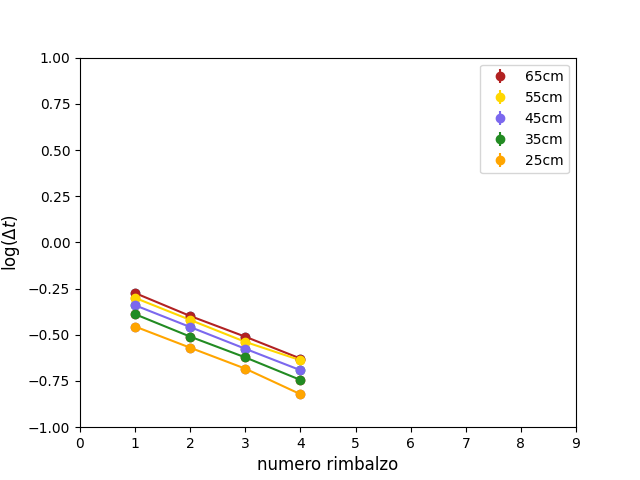
\includegraphics{Metodo2/computed_data/graficoLog_pallina3.png}
			} %close resize
		} %close centering
		\caption{Figura7:\(log\Delta t _{(n)}\) - pallina da tennis su gres porcellanato}
	\end{figure}
	
	\noindent Abbiamo ricavato il coefficiente angolare di ciascuna delle 5 rette tramite il metodo dei minimi quadrati.\\\\\\
	\begin{figure}[!ht]
		\captionsetup{labelformat=empty}
		\makebox[1 \textwidth][c]{       %centering table
			\resizebox{0.7 \textwidth}{!}{   %resize table
				%%% Creator: Matplotlib, PGF backend
%%
%% To include the figure in your LaTeX document, write
%%   \input{<filename>.pgf}
%%
%% Make sure the required packages are loaded in your preamble
%%   \usepackage{pgf}
%%
%% and, on pdftex
%%   \usepackage[utf8]{inputenc}\DeclareUnicodeCharacter{2212}{-}
%%
%% or, on luatex and xetex
%%   \usepackage{unicode-math}
%%
%% Figures using additional raster images can only be included by \input if
%% they are in the same directory as the main LaTeX file. For loading figures
%% from other directories you can use the `import` package
%%   \usepackage{import}
%%
%% and then include the figures with
%%   \import{<path to file>}{<filename>.pgf}
%%
%% Matplotlib used the following preamble
%%   \usepackage{fontspec}
%%   \setmainfont{DejaVuSerif.ttf}[Path=C:/Users/giuly/AppData/Local/Programs/Python/Python39/Lib/site-packages/matplotlib/mpl-data/fonts/ttf/]
%%   \setsansfont{DejaVuSans.ttf}[Path=C:/Users/giuly/AppData/Local/Programs/Python/Python39/Lib/site-packages/matplotlib/mpl-data/fonts/ttf/]
%%   \setmonofont{DejaVuSansMono.ttf}[Path=C:/Users/giuly/AppData/Local/Programs/Python/Python39/Lib/site-packages/matplotlib/mpl-data/fonts/ttf/]
%%
\begingroup%
\makeatletter%
\begin{pgfpicture}%
\pgfpathrectangle{\pgfpointorigin}{\pgfqpoint{6.400000in}{4.800000in}}%
\pgfusepath{use as bounding box, clip}%
\begin{pgfscope}%
\pgfsetbuttcap%
\pgfsetmiterjoin%
\definecolor{currentfill}{rgb}{1.000000,1.000000,1.000000}%
\pgfsetfillcolor{currentfill}%
\pgfsetlinewidth{0.000000pt}%
\definecolor{currentstroke}{rgb}{1.000000,1.000000,1.000000}%
\pgfsetstrokecolor{currentstroke}%
\pgfsetdash{}{0pt}%
\pgfpathmoveto{\pgfqpoint{0.000000in}{0.000000in}}%
\pgfpathlineto{\pgfqpoint{6.400000in}{0.000000in}}%
\pgfpathlineto{\pgfqpoint{6.400000in}{4.800000in}}%
\pgfpathlineto{\pgfqpoint{0.000000in}{4.800000in}}%
\pgfpathclose%
\pgfusepath{fill}%
\end{pgfscope}%
\begin{pgfscope}%
\pgfsetbuttcap%
\pgfsetmiterjoin%
\definecolor{currentfill}{rgb}{1.000000,1.000000,1.000000}%
\pgfsetfillcolor{currentfill}%
\pgfsetlinewidth{0.000000pt}%
\definecolor{currentstroke}{rgb}{0.000000,0.000000,0.000000}%
\pgfsetstrokecolor{currentstroke}%
\pgfsetstrokeopacity{0.000000}%
\pgfsetdash{}{0pt}%
\pgfpathmoveto{\pgfqpoint{0.800000in}{0.528000in}}%
\pgfpathlineto{\pgfqpoint{5.760000in}{0.528000in}}%
\pgfpathlineto{\pgfqpoint{5.760000in}{4.224000in}}%
\pgfpathlineto{\pgfqpoint{0.800000in}{4.224000in}}%
\pgfpathclose%
\pgfusepath{fill}%
\end{pgfscope}%
\begin{pgfscope}%
\pgfpathrectangle{\pgfqpoint{0.800000in}{0.528000in}}{\pgfqpoint{4.960000in}{3.696000in}}%
\pgfusepath{clip}%
\pgfsetbuttcap%
\pgfsetmiterjoin%
\definecolor{currentfill}{rgb}{0.400000,0.803922,0.666667}%
\pgfsetfillcolor{currentfill}%
\pgfsetfillopacity{0.800000}%
\pgfsetlinewidth{0.000000pt}%
\definecolor{currentstroke}{rgb}{0.000000,0.000000,0.000000}%
\pgfsetstrokecolor{currentstroke}%
\pgfsetstrokeopacity{0.800000}%
\pgfsetdash{}{0pt}%
\pgfpathmoveto{\pgfqpoint{1.025455in}{0.528000in}}%
\pgfpathlineto{\pgfqpoint{1.401212in}{0.528000in}}%
\pgfpathlineto{\pgfqpoint{1.401212in}{0.848000in}}%
\pgfpathlineto{\pgfqpoint{1.025455in}{0.848000in}}%
\pgfpathclose%
\pgfusepath{fill}%
\end{pgfscope}%
\begin{pgfscope}%
\pgfpathrectangle{\pgfqpoint{0.800000in}{0.528000in}}{\pgfqpoint{4.960000in}{3.696000in}}%
\pgfusepath{clip}%
\pgfsetbuttcap%
\pgfsetmiterjoin%
\definecolor{currentfill}{rgb}{0.400000,0.803922,0.666667}%
\pgfsetfillcolor{currentfill}%
\pgfsetfillopacity{0.800000}%
\pgfsetlinewidth{0.000000pt}%
\definecolor{currentstroke}{rgb}{0.000000,0.000000,0.000000}%
\pgfsetstrokecolor{currentstroke}%
\pgfsetstrokeopacity{0.800000}%
\pgfsetdash{}{0pt}%
\pgfpathmoveto{\pgfqpoint{1.401212in}{0.528000in}}%
\pgfpathlineto{\pgfqpoint{1.776970in}{0.528000in}}%
\pgfpathlineto{\pgfqpoint{1.776970in}{0.848000in}}%
\pgfpathlineto{\pgfqpoint{1.401212in}{0.848000in}}%
\pgfpathclose%
\pgfusepath{fill}%
\end{pgfscope}%
\begin{pgfscope}%
\pgfpathrectangle{\pgfqpoint{0.800000in}{0.528000in}}{\pgfqpoint{4.960000in}{3.696000in}}%
\pgfusepath{clip}%
\pgfsetbuttcap%
\pgfsetmiterjoin%
\definecolor{currentfill}{rgb}{0.400000,0.803922,0.666667}%
\pgfsetfillcolor{currentfill}%
\pgfsetfillopacity{0.800000}%
\pgfsetlinewidth{0.000000pt}%
\definecolor{currentstroke}{rgb}{0.000000,0.000000,0.000000}%
\pgfsetstrokecolor{currentstroke}%
\pgfsetstrokeopacity{0.800000}%
\pgfsetdash{}{0pt}%
\pgfpathmoveto{\pgfqpoint{1.776970in}{0.528000in}}%
\pgfpathlineto{\pgfqpoint{2.152727in}{0.528000in}}%
\pgfpathlineto{\pgfqpoint{2.152727in}{1.168000in}}%
\pgfpathlineto{\pgfqpoint{1.776970in}{1.168000in}}%
\pgfpathclose%
\pgfusepath{fill}%
\end{pgfscope}%
\begin{pgfscope}%
\pgfpathrectangle{\pgfqpoint{0.800000in}{0.528000in}}{\pgfqpoint{4.960000in}{3.696000in}}%
\pgfusepath{clip}%
\pgfsetbuttcap%
\pgfsetmiterjoin%
\definecolor{currentfill}{rgb}{0.400000,0.803922,0.666667}%
\pgfsetfillcolor{currentfill}%
\pgfsetfillopacity{0.800000}%
\pgfsetlinewidth{0.000000pt}%
\definecolor{currentstroke}{rgb}{0.000000,0.000000,0.000000}%
\pgfsetstrokecolor{currentstroke}%
\pgfsetstrokeopacity{0.800000}%
\pgfsetdash{}{0pt}%
\pgfpathmoveto{\pgfqpoint{2.152727in}{0.528000in}}%
\pgfpathlineto{\pgfqpoint{2.528485in}{0.528000in}}%
\pgfpathlineto{\pgfqpoint{2.528485in}{1.968000in}}%
\pgfpathlineto{\pgfqpoint{2.152727in}{1.968000in}}%
\pgfpathclose%
\pgfusepath{fill}%
\end{pgfscope}%
\begin{pgfscope}%
\pgfpathrectangle{\pgfqpoint{0.800000in}{0.528000in}}{\pgfqpoint{4.960000in}{3.696000in}}%
\pgfusepath{clip}%
\pgfsetbuttcap%
\pgfsetmiterjoin%
\definecolor{currentfill}{rgb}{0.400000,0.803922,0.666667}%
\pgfsetfillcolor{currentfill}%
\pgfsetfillopacity{0.800000}%
\pgfsetlinewidth{0.000000pt}%
\definecolor{currentstroke}{rgb}{0.000000,0.000000,0.000000}%
\pgfsetstrokecolor{currentstroke}%
\pgfsetstrokeopacity{0.800000}%
\pgfsetdash{}{0pt}%
\pgfpathmoveto{\pgfqpoint{2.528485in}{0.528000in}}%
\pgfpathlineto{\pgfqpoint{2.904242in}{0.528000in}}%
\pgfpathlineto{\pgfqpoint{2.904242in}{2.448000in}}%
\pgfpathlineto{\pgfqpoint{2.528485in}{2.448000in}}%
\pgfpathclose%
\pgfusepath{fill}%
\end{pgfscope}%
\begin{pgfscope}%
\pgfpathrectangle{\pgfqpoint{0.800000in}{0.528000in}}{\pgfqpoint{4.960000in}{3.696000in}}%
\pgfusepath{clip}%
\pgfsetbuttcap%
\pgfsetmiterjoin%
\definecolor{currentfill}{rgb}{0.400000,0.803922,0.666667}%
\pgfsetfillcolor{currentfill}%
\pgfsetfillopacity{0.800000}%
\pgfsetlinewidth{0.000000pt}%
\definecolor{currentstroke}{rgb}{0.000000,0.000000,0.000000}%
\pgfsetstrokecolor{currentstroke}%
\pgfsetstrokeopacity{0.800000}%
\pgfsetdash{}{0pt}%
\pgfpathmoveto{\pgfqpoint{2.904242in}{0.528000in}}%
\pgfpathlineto{\pgfqpoint{3.280000in}{0.528000in}}%
\pgfpathlineto{\pgfqpoint{3.280000in}{4.048000in}}%
\pgfpathlineto{\pgfqpoint{2.904242in}{4.048000in}}%
\pgfpathclose%
\pgfusepath{fill}%
\end{pgfscope}%
\begin{pgfscope}%
\pgfpathrectangle{\pgfqpoint{0.800000in}{0.528000in}}{\pgfqpoint{4.960000in}{3.696000in}}%
\pgfusepath{clip}%
\pgfsetbuttcap%
\pgfsetmiterjoin%
\definecolor{currentfill}{rgb}{0.400000,0.803922,0.666667}%
\pgfsetfillcolor{currentfill}%
\pgfsetfillopacity{0.800000}%
\pgfsetlinewidth{0.000000pt}%
\definecolor{currentstroke}{rgb}{0.000000,0.000000,0.000000}%
\pgfsetstrokecolor{currentstroke}%
\pgfsetstrokeopacity{0.800000}%
\pgfsetdash{}{0pt}%
\pgfpathmoveto{\pgfqpoint{3.280000in}{0.528000in}}%
\pgfpathlineto{\pgfqpoint{3.655758in}{0.528000in}}%
\pgfpathlineto{\pgfqpoint{3.655758in}{3.248000in}}%
\pgfpathlineto{\pgfqpoint{3.280000in}{3.248000in}}%
\pgfpathclose%
\pgfusepath{fill}%
\end{pgfscope}%
\begin{pgfscope}%
\pgfpathrectangle{\pgfqpoint{0.800000in}{0.528000in}}{\pgfqpoint{4.960000in}{3.696000in}}%
\pgfusepath{clip}%
\pgfsetbuttcap%
\pgfsetmiterjoin%
\definecolor{currentfill}{rgb}{0.400000,0.803922,0.666667}%
\pgfsetfillcolor{currentfill}%
\pgfsetfillopacity{0.800000}%
\pgfsetlinewidth{0.000000pt}%
\definecolor{currentstroke}{rgb}{0.000000,0.000000,0.000000}%
\pgfsetstrokecolor{currentstroke}%
\pgfsetstrokeopacity{0.800000}%
\pgfsetdash{}{0pt}%
\pgfpathmoveto{\pgfqpoint{3.655758in}{0.528000in}}%
\pgfpathlineto{\pgfqpoint{4.031515in}{0.528000in}}%
\pgfpathlineto{\pgfqpoint{4.031515in}{3.248000in}}%
\pgfpathlineto{\pgfqpoint{3.655758in}{3.248000in}}%
\pgfpathclose%
\pgfusepath{fill}%
\end{pgfscope}%
\begin{pgfscope}%
\pgfpathrectangle{\pgfqpoint{0.800000in}{0.528000in}}{\pgfqpoint{4.960000in}{3.696000in}}%
\pgfusepath{clip}%
\pgfsetbuttcap%
\pgfsetmiterjoin%
\definecolor{currentfill}{rgb}{0.400000,0.803922,0.666667}%
\pgfsetfillcolor{currentfill}%
\pgfsetfillopacity{0.800000}%
\pgfsetlinewidth{0.000000pt}%
\definecolor{currentstroke}{rgb}{0.000000,0.000000,0.000000}%
\pgfsetstrokecolor{currentstroke}%
\pgfsetstrokeopacity{0.800000}%
\pgfsetdash{}{0pt}%
\pgfpathmoveto{\pgfqpoint{4.031515in}{0.528000in}}%
\pgfpathlineto{\pgfqpoint{4.407273in}{0.528000in}}%
\pgfpathlineto{\pgfqpoint{4.407273in}{1.968000in}}%
\pgfpathlineto{\pgfqpoint{4.031515in}{1.968000in}}%
\pgfpathclose%
\pgfusepath{fill}%
\end{pgfscope}%
\begin{pgfscope}%
\pgfpathrectangle{\pgfqpoint{0.800000in}{0.528000in}}{\pgfqpoint{4.960000in}{3.696000in}}%
\pgfusepath{clip}%
\pgfsetbuttcap%
\pgfsetmiterjoin%
\definecolor{currentfill}{rgb}{0.400000,0.803922,0.666667}%
\pgfsetfillcolor{currentfill}%
\pgfsetfillopacity{0.800000}%
\pgfsetlinewidth{0.000000pt}%
\definecolor{currentstroke}{rgb}{0.000000,0.000000,0.000000}%
\pgfsetstrokecolor{currentstroke}%
\pgfsetstrokeopacity{0.800000}%
\pgfsetdash{}{0pt}%
\pgfpathmoveto{\pgfqpoint{4.407273in}{0.528000in}}%
\pgfpathlineto{\pgfqpoint{4.783030in}{0.528000in}}%
\pgfpathlineto{\pgfqpoint{4.783030in}{1.168000in}}%
\pgfpathlineto{\pgfqpoint{4.407273in}{1.168000in}}%
\pgfpathclose%
\pgfusepath{fill}%
\end{pgfscope}%
\begin{pgfscope}%
\pgfpathrectangle{\pgfqpoint{0.800000in}{0.528000in}}{\pgfqpoint{4.960000in}{3.696000in}}%
\pgfusepath{clip}%
\pgfsetbuttcap%
\pgfsetmiterjoin%
\definecolor{currentfill}{rgb}{0.400000,0.803922,0.666667}%
\pgfsetfillcolor{currentfill}%
\pgfsetfillopacity{0.800000}%
\pgfsetlinewidth{0.000000pt}%
\definecolor{currentstroke}{rgb}{0.000000,0.000000,0.000000}%
\pgfsetstrokecolor{currentstroke}%
\pgfsetstrokeopacity{0.800000}%
\pgfsetdash{}{0pt}%
\pgfpathmoveto{\pgfqpoint{4.783030in}{0.528000in}}%
\pgfpathlineto{\pgfqpoint{5.158788in}{0.528000in}}%
\pgfpathlineto{\pgfqpoint{5.158788in}{0.688000in}}%
\pgfpathlineto{\pgfqpoint{4.783030in}{0.688000in}}%
\pgfpathclose%
\pgfusepath{fill}%
\end{pgfscope}%
\begin{pgfscope}%
\pgfpathrectangle{\pgfqpoint{0.800000in}{0.528000in}}{\pgfqpoint{4.960000in}{3.696000in}}%
\pgfusepath{clip}%
\pgfsetbuttcap%
\pgfsetmiterjoin%
\definecolor{currentfill}{rgb}{0.400000,0.803922,0.666667}%
\pgfsetfillcolor{currentfill}%
\pgfsetfillopacity{0.800000}%
\pgfsetlinewidth{0.000000pt}%
\definecolor{currentstroke}{rgb}{0.000000,0.000000,0.000000}%
\pgfsetstrokecolor{currentstroke}%
\pgfsetstrokeopacity{0.800000}%
\pgfsetdash{}{0pt}%
\pgfpathmoveto{\pgfqpoint{5.158788in}{0.528000in}}%
\pgfpathlineto{\pgfqpoint{5.534545in}{0.528000in}}%
\pgfpathlineto{\pgfqpoint{5.534545in}{0.688000in}}%
\pgfpathlineto{\pgfqpoint{5.158788in}{0.688000in}}%
\pgfpathclose%
\pgfusepath{fill}%
\end{pgfscope}%
\begin{pgfscope}%
\pgfsetbuttcap%
\pgfsetroundjoin%
\definecolor{currentfill}{rgb}{0.000000,0.000000,0.000000}%
\pgfsetfillcolor{currentfill}%
\pgfsetlinewidth{0.803000pt}%
\definecolor{currentstroke}{rgb}{0.000000,0.000000,0.000000}%
\pgfsetstrokecolor{currentstroke}%
\pgfsetdash{}{0pt}%
\pgfsys@defobject{currentmarker}{\pgfqpoint{0.000000in}{-0.048611in}}{\pgfqpoint{0.000000in}{0.000000in}}{%
\pgfpathmoveto{\pgfqpoint{0.000000in}{0.000000in}}%
\pgfpathlineto{\pgfqpoint{0.000000in}{-0.048611in}}%
\pgfusepath{stroke,fill}%
}%
\begin{pgfscope}%
\pgfsys@transformshift{1.025455in}{0.528000in}%
\pgfsys@useobject{currentmarker}{}%
\end{pgfscope}%
\end{pgfscope}%
\begin{pgfscope}%
\definecolor{textcolor}{rgb}{0.000000,0.000000,0.000000}%
\pgfsetstrokecolor{textcolor}%
\pgfsetfillcolor{textcolor}%
\pgftext[x=1.025455in,y=0.430778in,,top]{\color{textcolor}\sffamily\fontsize{10.000000}{12.000000}\selectfont 1.30}%
\end{pgfscope}%
\begin{pgfscope}%
\pgfsetbuttcap%
\pgfsetroundjoin%
\definecolor{currentfill}{rgb}{0.000000,0.000000,0.000000}%
\pgfsetfillcolor{currentfill}%
\pgfsetlinewidth{0.803000pt}%
\definecolor{currentstroke}{rgb}{0.000000,0.000000,0.000000}%
\pgfsetstrokecolor{currentstroke}%
\pgfsetdash{}{0pt}%
\pgfsys@defobject{currentmarker}{\pgfqpoint{0.000000in}{-0.048611in}}{\pgfqpoint{0.000000in}{0.000000in}}{%
\pgfpathmoveto{\pgfqpoint{0.000000in}{0.000000in}}%
\pgfpathlineto{\pgfqpoint{0.000000in}{-0.048611in}}%
\pgfusepath{stroke,fill}%
}%
\begin{pgfscope}%
\pgfsys@transformshift{1.589091in}{0.528000in}%
\pgfsys@useobject{currentmarker}{}%
\end{pgfscope}%
\end{pgfscope}%
\begin{pgfscope}%
\definecolor{textcolor}{rgb}{0.000000,0.000000,0.000000}%
\pgfsetstrokecolor{textcolor}%
\pgfsetfillcolor{textcolor}%
\pgftext[x=1.589091in,y=0.430778in,,top]{\color{textcolor}\sffamily\fontsize{10.000000}{12.000000}\selectfont 1.35}%
\end{pgfscope}%
\begin{pgfscope}%
\pgfsetbuttcap%
\pgfsetroundjoin%
\definecolor{currentfill}{rgb}{0.000000,0.000000,0.000000}%
\pgfsetfillcolor{currentfill}%
\pgfsetlinewidth{0.803000pt}%
\definecolor{currentstroke}{rgb}{0.000000,0.000000,0.000000}%
\pgfsetstrokecolor{currentstroke}%
\pgfsetdash{}{0pt}%
\pgfsys@defobject{currentmarker}{\pgfqpoint{0.000000in}{-0.048611in}}{\pgfqpoint{0.000000in}{0.000000in}}{%
\pgfpathmoveto{\pgfqpoint{0.000000in}{0.000000in}}%
\pgfpathlineto{\pgfqpoint{0.000000in}{-0.048611in}}%
\pgfusepath{stroke,fill}%
}%
\begin{pgfscope}%
\pgfsys@transformshift{2.152727in}{0.528000in}%
\pgfsys@useobject{currentmarker}{}%
\end{pgfscope}%
\end{pgfscope}%
\begin{pgfscope}%
\definecolor{textcolor}{rgb}{0.000000,0.000000,0.000000}%
\pgfsetstrokecolor{textcolor}%
\pgfsetfillcolor{textcolor}%
\pgftext[x=2.152727in,y=0.430778in,,top]{\color{textcolor}\sffamily\fontsize{10.000000}{12.000000}\selectfont 1.40}%
\end{pgfscope}%
\begin{pgfscope}%
\pgfsetbuttcap%
\pgfsetroundjoin%
\definecolor{currentfill}{rgb}{0.000000,0.000000,0.000000}%
\pgfsetfillcolor{currentfill}%
\pgfsetlinewidth{0.803000pt}%
\definecolor{currentstroke}{rgb}{0.000000,0.000000,0.000000}%
\pgfsetstrokecolor{currentstroke}%
\pgfsetdash{}{0pt}%
\pgfsys@defobject{currentmarker}{\pgfqpoint{0.000000in}{-0.048611in}}{\pgfqpoint{0.000000in}{0.000000in}}{%
\pgfpathmoveto{\pgfqpoint{0.000000in}{0.000000in}}%
\pgfpathlineto{\pgfqpoint{0.000000in}{-0.048611in}}%
\pgfusepath{stroke,fill}%
}%
\begin{pgfscope}%
\pgfsys@transformshift{2.716364in}{0.528000in}%
\pgfsys@useobject{currentmarker}{}%
\end{pgfscope}%
\end{pgfscope}%
\begin{pgfscope}%
\definecolor{textcolor}{rgb}{0.000000,0.000000,0.000000}%
\pgfsetstrokecolor{textcolor}%
\pgfsetfillcolor{textcolor}%
\pgftext[x=2.716364in,y=0.430778in,,top]{\color{textcolor}\sffamily\fontsize{10.000000}{12.000000}\selectfont 1.45}%
\end{pgfscope}%
\begin{pgfscope}%
\pgfsetbuttcap%
\pgfsetroundjoin%
\definecolor{currentfill}{rgb}{0.000000,0.000000,0.000000}%
\pgfsetfillcolor{currentfill}%
\pgfsetlinewidth{0.803000pt}%
\definecolor{currentstroke}{rgb}{0.000000,0.000000,0.000000}%
\pgfsetstrokecolor{currentstroke}%
\pgfsetdash{}{0pt}%
\pgfsys@defobject{currentmarker}{\pgfqpoint{0.000000in}{-0.048611in}}{\pgfqpoint{0.000000in}{0.000000in}}{%
\pgfpathmoveto{\pgfqpoint{0.000000in}{0.000000in}}%
\pgfpathlineto{\pgfqpoint{0.000000in}{-0.048611in}}%
\pgfusepath{stroke,fill}%
}%
\begin{pgfscope}%
\pgfsys@transformshift{3.280000in}{0.528000in}%
\pgfsys@useobject{currentmarker}{}%
\end{pgfscope}%
\end{pgfscope}%
\begin{pgfscope}%
\definecolor{textcolor}{rgb}{0.000000,0.000000,0.000000}%
\pgfsetstrokecolor{textcolor}%
\pgfsetfillcolor{textcolor}%
\pgftext[x=3.280000in,y=0.430778in,,top]{\color{textcolor}\sffamily\fontsize{10.000000}{12.000000}\selectfont 1.50}%
\end{pgfscope}%
\begin{pgfscope}%
\pgfsetbuttcap%
\pgfsetroundjoin%
\definecolor{currentfill}{rgb}{0.000000,0.000000,0.000000}%
\pgfsetfillcolor{currentfill}%
\pgfsetlinewidth{0.803000pt}%
\definecolor{currentstroke}{rgb}{0.000000,0.000000,0.000000}%
\pgfsetstrokecolor{currentstroke}%
\pgfsetdash{}{0pt}%
\pgfsys@defobject{currentmarker}{\pgfqpoint{0.000000in}{-0.048611in}}{\pgfqpoint{0.000000in}{0.000000in}}{%
\pgfpathmoveto{\pgfqpoint{0.000000in}{0.000000in}}%
\pgfpathlineto{\pgfqpoint{0.000000in}{-0.048611in}}%
\pgfusepath{stroke,fill}%
}%
\begin{pgfscope}%
\pgfsys@transformshift{3.843636in}{0.528000in}%
\pgfsys@useobject{currentmarker}{}%
\end{pgfscope}%
\end{pgfscope}%
\begin{pgfscope}%
\definecolor{textcolor}{rgb}{0.000000,0.000000,0.000000}%
\pgfsetstrokecolor{textcolor}%
\pgfsetfillcolor{textcolor}%
\pgftext[x=3.843636in,y=0.430778in,,top]{\color{textcolor}\sffamily\fontsize{10.000000}{12.000000}\selectfont 1.55}%
\end{pgfscope}%
\begin{pgfscope}%
\pgfsetbuttcap%
\pgfsetroundjoin%
\definecolor{currentfill}{rgb}{0.000000,0.000000,0.000000}%
\pgfsetfillcolor{currentfill}%
\pgfsetlinewidth{0.803000pt}%
\definecolor{currentstroke}{rgb}{0.000000,0.000000,0.000000}%
\pgfsetstrokecolor{currentstroke}%
\pgfsetdash{}{0pt}%
\pgfsys@defobject{currentmarker}{\pgfqpoint{0.000000in}{-0.048611in}}{\pgfqpoint{0.000000in}{0.000000in}}{%
\pgfpathmoveto{\pgfqpoint{0.000000in}{0.000000in}}%
\pgfpathlineto{\pgfqpoint{0.000000in}{-0.048611in}}%
\pgfusepath{stroke,fill}%
}%
\begin{pgfscope}%
\pgfsys@transformshift{4.407273in}{0.528000in}%
\pgfsys@useobject{currentmarker}{}%
\end{pgfscope}%
\end{pgfscope}%
\begin{pgfscope}%
\definecolor{textcolor}{rgb}{0.000000,0.000000,0.000000}%
\pgfsetstrokecolor{textcolor}%
\pgfsetfillcolor{textcolor}%
\pgftext[x=4.407273in,y=0.430778in,,top]{\color{textcolor}\sffamily\fontsize{10.000000}{12.000000}\selectfont 1.60}%
\end{pgfscope}%
\begin{pgfscope}%
\pgfsetbuttcap%
\pgfsetroundjoin%
\definecolor{currentfill}{rgb}{0.000000,0.000000,0.000000}%
\pgfsetfillcolor{currentfill}%
\pgfsetlinewidth{0.803000pt}%
\definecolor{currentstroke}{rgb}{0.000000,0.000000,0.000000}%
\pgfsetstrokecolor{currentstroke}%
\pgfsetdash{}{0pt}%
\pgfsys@defobject{currentmarker}{\pgfqpoint{0.000000in}{-0.048611in}}{\pgfqpoint{0.000000in}{0.000000in}}{%
\pgfpathmoveto{\pgfqpoint{0.000000in}{0.000000in}}%
\pgfpathlineto{\pgfqpoint{0.000000in}{-0.048611in}}%
\pgfusepath{stroke,fill}%
}%
\begin{pgfscope}%
\pgfsys@transformshift{4.970909in}{0.528000in}%
\pgfsys@useobject{currentmarker}{}%
\end{pgfscope}%
\end{pgfscope}%
\begin{pgfscope}%
\definecolor{textcolor}{rgb}{0.000000,0.000000,0.000000}%
\pgfsetstrokecolor{textcolor}%
\pgfsetfillcolor{textcolor}%
\pgftext[x=4.970909in,y=0.430778in,,top]{\color{textcolor}\sffamily\fontsize{10.000000}{12.000000}\selectfont 1.65}%
\end{pgfscope}%
\begin{pgfscope}%
\pgfsetbuttcap%
\pgfsetroundjoin%
\definecolor{currentfill}{rgb}{0.000000,0.000000,0.000000}%
\pgfsetfillcolor{currentfill}%
\pgfsetlinewidth{0.803000pt}%
\definecolor{currentstroke}{rgb}{0.000000,0.000000,0.000000}%
\pgfsetstrokecolor{currentstroke}%
\pgfsetdash{}{0pt}%
\pgfsys@defobject{currentmarker}{\pgfqpoint{0.000000in}{-0.048611in}}{\pgfqpoint{0.000000in}{0.000000in}}{%
\pgfpathmoveto{\pgfqpoint{0.000000in}{0.000000in}}%
\pgfpathlineto{\pgfqpoint{0.000000in}{-0.048611in}}%
\pgfusepath{stroke,fill}%
}%
\begin{pgfscope}%
\pgfsys@transformshift{5.534545in}{0.528000in}%
\pgfsys@useobject{currentmarker}{}%
\end{pgfscope}%
\end{pgfscope}%
\begin{pgfscope}%
\definecolor{textcolor}{rgb}{0.000000,0.000000,0.000000}%
\pgfsetstrokecolor{textcolor}%
\pgfsetfillcolor{textcolor}%
\pgftext[x=5.534545in,y=0.430778in,,top]{\color{textcolor}\sffamily\fontsize{10.000000}{12.000000}\selectfont 1.70}%
\end{pgfscope}%
\begin{pgfscope}%
\definecolor{textcolor}{rgb}{0.000000,0.000000,0.000000}%
\pgfsetstrokecolor{textcolor}%
\pgfsetfillcolor{textcolor}%
\pgftext[x=3.280000in,y=0.240809in,,top]{\color{textcolor}\sffamily\fontsize{10.000000}{12.000000}\selectfont \(\displaystyle x_k\) (s)}%
\end{pgfscope}%
\begin{pgfscope}%
\pgfsetbuttcap%
\pgfsetroundjoin%
\definecolor{currentfill}{rgb}{0.000000,0.000000,0.000000}%
\pgfsetfillcolor{currentfill}%
\pgfsetlinewidth{0.803000pt}%
\definecolor{currentstroke}{rgb}{0.000000,0.000000,0.000000}%
\pgfsetstrokecolor{currentstroke}%
\pgfsetdash{}{0pt}%
\pgfsys@defobject{currentmarker}{\pgfqpoint{-0.048611in}{0.000000in}}{\pgfqpoint{-0.000000in}{0.000000in}}{%
\pgfpathmoveto{\pgfqpoint{-0.000000in}{0.000000in}}%
\pgfpathlineto{\pgfqpoint{-0.048611in}{0.000000in}}%
\pgfusepath{stroke,fill}%
}%
\begin{pgfscope}%
\pgfsys@transformshift{0.800000in}{0.528000in}%
\pgfsys@useobject{currentmarker}{}%
\end{pgfscope}%
\end{pgfscope}%
\begin{pgfscope}%
\definecolor{textcolor}{rgb}{0.000000,0.000000,0.000000}%
\pgfsetstrokecolor{textcolor}%
\pgfsetfillcolor{textcolor}%
\pgftext[x=0.614412in, y=0.475238in, left, base]{\color{textcolor}\sffamily\fontsize{10.000000}{12.000000}\selectfont 0}%
\end{pgfscope}%
\begin{pgfscope}%
\pgfsetbuttcap%
\pgfsetroundjoin%
\definecolor{currentfill}{rgb}{0.000000,0.000000,0.000000}%
\pgfsetfillcolor{currentfill}%
\pgfsetlinewidth{0.803000pt}%
\definecolor{currentstroke}{rgb}{0.000000,0.000000,0.000000}%
\pgfsetstrokecolor{currentstroke}%
\pgfsetdash{}{0pt}%
\pgfsys@defobject{currentmarker}{\pgfqpoint{-0.048611in}{0.000000in}}{\pgfqpoint{-0.000000in}{0.000000in}}{%
\pgfpathmoveto{\pgfqpoint{-0.000000in}{0.000000in}}%
\pgfpathlineto{\pgfqpoint{-0.048611in}{0.000000in}}%
\pgfusepath{stroke,fill}%
}%
\begin{pgfscope}%
\pgfsys@transformshift{0.800000in}{1.061333in}%
\pgfsys@useobject{currentmarker}{}%
\end{pgfscope}%
\end{pgfscope}%
\begin{pgfscope}%
\definecolor{textcolor}{rgb}{0.000000,0.000000,0.000000}%
\pgfsetstrokecolor{textcolor}%
\pgfsetfillcolor{textcolor}%
\pgftext[x=0.614412in, y=1.008572in, left, base]{\color{textcolor}\sffamily\fontsize{10.000000}{12.000000}\selectfont 1}%
\end{pgfscope}%
\begin{pgfscope}%
\pgfsetbuttcap%
\pgfsetroundjoin%
\definecolor{currentfill}{rgb}{0.000000,0.000000,0.000000}%
\pgfsetfillcolor{currentfill}%
\pgfsetlinewidth{0.803000pt}%
\definecolor{currentstroke}{rgb}{0.000000,0.000000,0.000000}%
\pgfsetstrokecolor{currentstroke}%
\pgfsetdash{}{0pt}%
\pgfsys@defobject{currentmarker}{\pgfqpoint{-0.048611in}{0.000000in}}{\pgfqpoint{-0.000000in}{0.000000in}}{%
\pgfpathmoveto{\pgfqpoint{-0.000000in}{0.000000in}}%
\pgfpathlineto{\pgfqpoint{-0.048611in}{0.000000in}}%
\pgfusepath{stroke,fill}%
}%
\begin{pgfscope}%
\pgfsys@transformshift{0.800000in}{1.594667in}%
\pgfsys@useobject{currentmarker}{}%
\end{pgfscope}%
\end{pgfscope}%
\begin{pgfscope}%
\definecolor{textcolor}{rgb}{0.000000,0.000000,0.000000}%
\pgfsetstrokecolor{textcolor}%
\pgfsetfillcolor{textcolor}%
\pgftext[x=0.614412in, y=1.541905in, left, base]{\color{textcolor}\sffamily\fontsize{10.000000}{12.000000}\selectfont 2}%
\end{pgfscope}%
\begin{pgfscope}%
\pgfsetbuttcap%
\pgfsetroundjoin%
\definecolor{currentfill}{rgb}{0.000000,0.000000,0.000000}%
\pgfsetfillcolor{currentfill}%
\pgfsetlinewidth{0.803000pt}%
\definecolor{currentstroke}{rgb}{0.000000,0.000000,0.000000}%
\pgfsetstrokecolor{currentstroke}%
\pgfsetdash{}{0pt}%
\pgfsys@defobject{currentmarker}{\pgfqpoint{-0.048611in}{0.000000in}}{\pgfqpoint{-0.000000in}{0.000000in}}{%
\pgfpathmoveto{\pgfqpoint{-0.000000in}{0.000000in}}%
\pgfpathlineto{\pgfqpoint{-0.048611in}{0.000000in}}%
\pgfusepath{stroke,fill}%
}%
\begin{pgfscope}%
\pgfsys@transformshift{0.800000in}{2.128000in}%
\pgfsys@useobject{currentmarker}{}%
\end{pgfscope}%
\end{pgfscope}%
\begin{pgfscope}%
\definecolor{textcolor}{rgb}{0.000000,0.000000,0.000000}%
\pgfsetstrokecolor{textcolor}%
\pgfsetfillcolor{textcolor}%
\pgftext[x=0.614412in, y=2.075238in, left, base]{\color{textcolor}\sffamily\fontsize{10.000000}{12.000000}\selectfont 3}%
\end{pgfscope}%
\begin{pgfscope}%
\pgfsetbuttcap%
\pgfsetroundjoin%
\definecolor{currentfill}{rgb}{0.000000,0.000000,0.000000}%
\pgfsetfillcolor{currentfill}%
\pgfsetlinewidth{0.803000pt}%
\definecolor{currentstroke}{rgb}{0.000000,0.000000,0.000000}%
\pgfsetstrokecolor{currentstroke}%
\pgfsetdash{}{0pt}%
\pgfsys@defobject{currentmarker}{\pgfqpoint{-0.048611in}{0.000000in}}{\pgfqpoint{-0.000000in}{0.000000in}}{%
\pgfpathmoveto{\pgfqpoint{-0.000000in}{0.000000in}}%
\pgfpathlineto{\pgfqpoint{-0.048611in}{0.000000in}}%
\pgfusepath{stroke,fill}%
}%
\begin{pgfscope}%
\pgfsys@transformshift{0.800000in}{2.661333in}%
\pgfsys@useobject{currentmarker}{}%
\end{pgfscope}%
\end{pgfscope}%
\begin{pgfscope}%
\definecolor{textcolor}{rgb}{0.000000,0.000000,0.000000}%
\pgfsetstrokecolor{textcolor}%
\pgfsetfillcolor{textcolor}%
\pgftext[x=0.614412in, y=2.608572in, left, base]{\color{textcolor}\sffamily\fontsize{10.000000}{12.000000}\selectfont 4}%
\end{pgfscope}%
\begin{pgfscope}%
\pgfsetbuttcap%
\pgfsetroundjoin%
\definecolor{currentfill}{rgb}{0.000000,0.000000,0.000000}%
\pgfsetfillcolor{currentfill}%
\pgfsetlinewidth{0.803000pt}%
\definecolor{currentstroke}{rgb}{0.000000,0.000000,0.000000}%
\pgfsetstrokecolor{currentstroke}%
\pgfsetdash{}{0pt}%
\pgfsys@defobject{currentmarker}{\pgfqpoint{-0.048611in}{0.000000in}}{\pgfqpoint{-0.000000in}{0.000000in}}{%
\pgfpathmoveto{\pgfqpoint{-0.000000in}{0.000000in}}%
\pgfpathlineto{\pgfqpoint{-0.048611in}{0.000000in}}%
\pgfusepath{stroke,fill}%
}%
\begin{pgfscope}%
\pgfsys@transformshift{0.800000in}{3.194667in}%
\pgfsys@useobject{currentmarker}{}%
\end{pgfscope}%
\end{pgfscope}%
\begin{pgfscope}%
\definecolor{textcolor}{rgb}{0.000000,0.000000,0.000000}%
\pgfsetstrokecolor{textcolor}%
\pgfsetfillcolor{textcolor}%
\pgftext[x=0.614412in, y=3.141905in, left, base]{\color{textcolor}\sffamily\fontsize{10.000000}{12.000000}\selectfont 5}%
\end{pgfscope}%
\begin{pgfscope}%
\pgfsetbuttcap%
\pgfsetroundjoin%
\definecolor{currentfill}{rgb}{0.000000,0.000000,0.000000}%
\pgfsetfillcolor{currentfill}%
\pgfsetlinewidth{0.803000pt}%
\definecolor{currentstroke}{rgb}{0.000000,0.000000,0.000000}%
\pgfsetstrokecolor{currentstroke}%
\pgfsetdash{}{0pt}%
\pgfsys@defobject{currentmarker}{\pgfqpoint{-0.048611in}{0.000000in}}{\pgfqpoint{-0.000000in}{0.000000in}}{%
\pgfpathmoveto{\pgfqpoint{-0.000000in}{0.000000in}}%
\pgfpathlineto{\pgfqpoint{-0.048611in}{0.000000in}}%
\pgfusepath{stroke,fill}%
}%
\begin{pgfscope}%
\pgfsys@transformshift{0.800000in}{3.728000in}%
\pgfsys@useobject{currentmarker}{}%
\end{pgfscope}%
\end{pgfscope}%
\begin{pgfscope}%
\definecolor{textcolor}{rgb}{0.000000,0.000000,0.000000}%
\pgfsetstrokecolor{textcolor}%
\pgfsetfillcolor{textcolor}%
\pgftext[x=0.614412in, y=3.675238in, left, base]{\color{textcolor}\sffamily\fontsize{10.000000}{12.000000}\selectfont 6}%
\end{pgfscope}%
\begin{pgfscope}%
\definecolor{textcolor}{rgb}{0.000000,0.000000,0.000000}%
\pgfsetstrokecolor{textcolor}%
\pgfsetfillcolor{textcolor}%
\pgftext[x=0.558857in,y=2.376000in,,bottom,rotate=90.000000]{\color{textcolor}\sffamily\fontsize{10.000000}{12.000000}\selectfont Densità di Frequenza}%
\end{pgfscope}%
\begin{pgfscope}%
\pgfpathrectangle{\pgfqpoint{0.800000in}{0.528000in}}{\pgfqpoint{4.960000in}{3.696000in}}%
\pgfusepath{clip}%
\pgfsetrectcap%
\pgfsetroundjoin%
\pgfsetlinewidth{1.505625pt}%
\definecolor{currentstroke}{rgb}{1.000000,0.549020,0.000000}%
\pgfsetstrokecolor{currentstroke}%
\pgfsetdash{}{0pt}%
\pgfpathmoveto{\pgfqpoint{1.025455in}{0.574044in}}%
\pgfpathlineto{\pgfqpoint{1.117477in}{0.593003in}}%
\pgfpathlineto{\pgfqpoint{1.209499in}{0.618431in}}%
\pgfpathlineto{\pgfqpoint{1.301521in}{0.651974in}}%
\pgfpathlineto{\pgfqpoint{1.393544in}{0.695485in}}%
\pgfpathlineto{\pgfqpoint{1.485566in}{0.750973in}}%
\pgfpathlineto{\pgfqpoint{1.577588in}{0.820521in}}%
\pgfpathlineto{\pgfqpoint{1.669610in}{0.906175in}}%
\pgfpathlineto{\pgfqpoint{1.761633in}{1.009791in}}%
\pgfpathlineto{\pgfqpoint{1.853655in}{1.132860in}}%
\pgfpathlineto{\pgfqpoint{1.945677in}{1.276309in}}%
\pgfpathlineto{\pgfqpoint{2.037699in}{1.440300in}}%
\pgfpathlineto{\pgfqpoint{2.129722in}{1.624034in}}%
\pgfpathlineto{\pgfqpoint{2.221744in}{1.825600in}}%
\pgfpathlineto{\pgfqpoint{2.313766in}{2.041867in}}%
\pgfpathlineto{\pgfqpoint{2.405788in}{2.268464in}}%
\pgfpathlineto{\pgfqpoint{2.497811in}{2.499842in}}%
\pgfpathlineto{\pgfqpoint{2.589833in}{2.729454in}}%
\pgfpathlineto{\pgfqpoint{2.681855in}{2.950017in}}%
\pgfpathlineto{\pgfqpoint{2.773878in}{3.153881in}}%
\pgfpathlineto{\pgfqpoint{2.865900in}{3.333452in}}%
\pgfpathlineto{\pgfqpoint{2.957922in}{3.481663in}}%
\pgfpathlineto{\pgfqpoint{3.049944in}{3.592427in}}%
\pgfpathlineto{\pgfqpoint{3.141967in}{3.661053in}}%
\pgfpathlineto{\pgfqpoint{3.233989in}{3.684577in}}%
\pgfpathlineto{\pgfqpoint{3.326011in}{3.661972in}}%
\pgfpathlineto{\pgfqpoint{3.418033in}{3.594225in}}%
\pgfpathlineto{\pgfqpoint{3.510056in}{3.484264in}}%
\pgfpathlineto{\pgfqpoint{3.602078in}{3.336746in}}%
\pgfpathlineto{\pgfqpoint{3.694100in}{3.157735in}}%
\pgfpathlineto{\pgfqpoint{3.786122in}{2.954284in}}%
\pgfpathlineto{\pgfqpoint{3.878145in}{2.733979in}}%
\pgfpathlineto{\pgfqpoint{3.970167in}{2.504475in}}%
\pgfpathlineto{\pgfqpoint{4.062189in}{2.273065in}}%
\pgfpathlineto{\pgfqpoint{4.154212in}{2.046315in}}%
\pgfpathlineto{\pgfqpoint{4.246234in}{1.829794in}}%
\pgfpathlineto{\pgfqpoint{4.338256in}{1.627899in}}%
\pgfpathlineto{\pgfqpoint{4.430278in}{1.443785in}}%
\pgfpathlineto{\pgfqpoint{4.522301in}{1.279389in}}%
\pgfpathlineto{\pgfqpoint{4.614323in}{1.135527in}}%
\pgfpathlineto{\pgfqpoint{4.706345in}{1.012058in}}%
\pgfpathlineto{\pgfqpoint{4.798367in}{0.908066in}}%
\pgfpathlineto{\pgfqpoint{4.890390in}{0.822070in}}%
\pgfpathlineto{\pgfqpoint{4.982412in}{0.752219in}}%
\pgfpathlineto{\pgfqpoint{5.074434in}{0.696471in}}%
\pgfpathlineto{\pgfqpoint{5.166456in}{0.652740in}}%
\pgfpathlineto{\pgfqpoint{5.258479in}{0.619016in}}%
\pgfpathlineto{\pgfqpoint{5.350501in}{0.593443in}}%
\pgfpathlineto{\pgfqpoint{5.442523in}{0.574370in}}%
\pgfpathlineto{\pgfqpoint{5.534545in}{0.560377in}}%
\pgfusepath{stroke}%
\end{pgfscope}%
\begin{pgfscope}%
\pgfsetrectcap%
\pgfsetmiterjoin%
\pgfsetlinewidth{0.803000pt}%
\definecolor{currentstroke}{rgb}{0.000000,0.000000,0.000000}%
\pgfsetstrokecolor{currentstroke}%
\pgfsetdash{}{0pt}%
\pgfpathmoveto{\pgfqpoint{0.800000in}{0.528000in}}%
\pgfpathlineto{\pgfqpoint{0.800000in}{4.224000in}}%
\pgfusepath{stroke}%
\end{pgfscope}%
\begin{pgfscope}%
\pgfsetrectcap%
\pgfsetmiterjoin%
\pgfsetlinewidth{0.803000pt}%
\definecolor{currentstroke}{rgb}{0.000000,0.000000,0.000000}%
\pgfsetstrokecolor{currentstroke}%
\pgfsetdash{}{0pt}%
\pgfpathmoveto{\pgfqpoint{5.760000in}{0.528000in}}%
\pgfpathlineto{\pgfqpoint{5.760000in}{4.224000in}}%
\pgfusepath{stroke}%
\end{pgfscope}%
\begin{pgfscope}%
\pgfsetrectcap%
\pgfsetmiterjoin%
\pgfsetlinewidth{0.803000pt}%
\definecolor{currentstroke}{rgb}{0.000000,0.000000,0.000000}%
\pgfsetstrokecolor{currentstroke}%
\pgfsetdash{}{0pt}%
\pgfpathmoveto{\pgfqpoint{0.800000in}{0.528000in}}%
\pgfpathlineto{\pgfqpoint{5.760000in}{0.528000in}}%
\pgfusepath{stroke}%
\end{pgfscope}%
\begin{pgfscope}%
\pgfsetrectcap%
\pgfsetmiterjoin%
\pgfsetlinewidth{0.803000pt}%
\definecolor{currentstroke}{rgb}{0.000000,0.000000,0.000000}%
\pgfsetstrokecolor{currentstroke}%
\pgfsetdash{}{0pt}%
\pgfpathmoveto{\pgfqpoint{0.800000in}{4.224000in}}%
\pgfpathlineto{\pgfqpoint{5.760000in}{4.224000in}}%
\pgfusepath{stroke}%
\end{pgfscope}%
\begin{pgfscope}%
\pgfsetbuttcap%
\pgfsetmiterjoin%
\definecolor{currentfill}{rgb}{1.000000,1.000000,1.000000}%
\pgfsetfillcolor{currentfill}%
\pgfsetfillopacity{0.800000}%
\pgfsetlinewidth{1.003750pt}%
\definecolor{currentstroke}{rgb}{0.800000,0.800000,0.800000}%
\pgfsetstrokecolor{currentstroke}%
\pgfsetstrokeopacity{0.800000}%
\pgfsetdash{}{0pt}%
\pgfpathmoveto{\pgfqpoint{4.613473in}{3.690899in}}%
\pgfpathlineto{\pgfqpoint{5.662778in}{3.690899in}}%
\pgfpathquadraticcurveto{\pgfqpoint{5.690556in}{3.690899in}}{\pgfqpoint{5.690556in}{3.718677in}}%
\pgfpathlineto{\pgfqpoint{5.690556in}{4.126778in}}%
\pgfpathquadraticcurveto{\pgfqpoint{5.690556in}{4.154556in}}{\pgfqpoint{5.662778in}{4.154556in}}%
\pgfpathlineto{\pgfqpoint{4.613473in}{4.154556in}}%
\pgfpathquadraticcurveto{\pgfqpoint{4.585695in}{4.154556in}}{\pgfqpoint{4.585695in}{4.126778in}}%
\pgfpathlineto{\pgfqpoint{4.585695in}{3.718677in}}%
\pgfpathquadraticcurveto{\pgfqpoint{4.585695in}{3.690899in}}{\pgfqpoint{4.613473in}{3.690899in}}%
\pgfpathclose%
\pgfusepath{stroke,fill}%
\end{pgfscope}%
\begin{pgfscope}%
\pgfsetrectcap%
\pgfsetroundjoin%
\pgfsetlinewidth{1.505625pt}%
\definecolor{currentstroke}{rgb}{1.000000,0.549020,0.000000}%
\pgfsetstrokecolor{currentstroke}%
\pgfsetdash{}{0pt}%
\pgfpathmoveto{\pgfqpoint{4.641251in}{4.033645in}}%
\pgfpathlineto{\pgfqpoint{4.919029in}{4.033645in}}%
\pgfusepath{stroke}%
\end{pgfscope}%
\begin{pgfscope}%
\definecolor{textcolor}{rgb}{0.000000,0.000000,0.000000}%
\pgfsetstrokecolor{textcolor}%
\pgfsetfillcolor{textcolor}%
\pgftext[x=5.030140in,y=3.985034in,left,base]{\color{textcolor}\sffamily\fontsize{10.000000}{12.000000}\selectfont \(\displaystyle G(x;\bar{T},\sigma)\)}%
\end{pgfscope}%
\begin{pgfscope}%
\pgfsetbuttcap%
\pgfsetmiterjoin%
\definecolor{currentfill}{rgb}{0.400000,0.803922,0.666667}%
\pgfsetfillcolor{currentfill}%
\pgfsetfillopacity{0.800000}%
\pgfsetlinewidth{0.000000pt}%
\definecolor{currentstroke}{rgb}{0.000000,0.000000,0.000000}%
\pgfsetstrokecolor{currentstroke}%
\pgfsetstrokeopacity{0.800000}%
\pgfsetdash{}{0pt}%
\pgfpathmoveto{\pgfqpoint{4.641251in}{3.775344in}}%
\pgfpathlineto{\pgfqpoint{4.919029in}{3.775344in}}%
\pgfpathlineto{\pgfqpoint{4.919029in}{3.872567in}}%
\pgfpathlineto{\pgfqpoint{4.641251in}{3.872567in}}%
\pgfpathclose%
\pgfusepath{fill}%
\end{pgfscope}%
\begin{pgfscope}%
\definecolor{textcolor}{rgb}{0.000000,0.000000,0.000000}%
\pgfsetstrokecolor{textcolor}%
\pgfsetfillcolor{textcolor}%
\pgftext[x=5.030140in,y=3.775344in,left,base]{\color{textcolor}\sffamily\fontsize{10.000000}{12.000000}\selectfont data}%
\end{pgfscope}%
\end{pgfpicture}%
\makeatother%
\endgroup%

				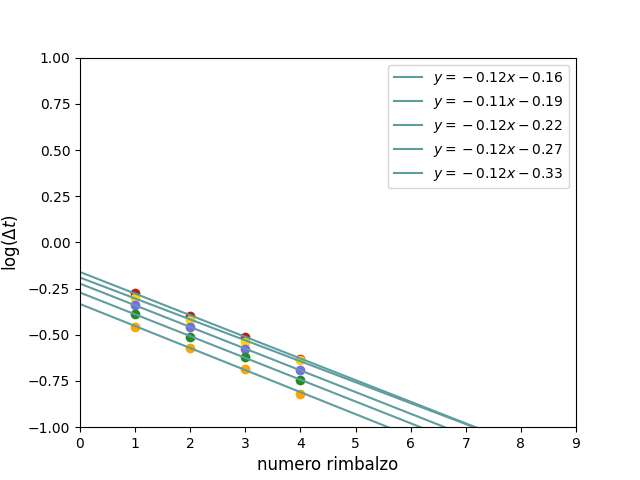
\includegraphics{Metodo2/computed_data/graficoLog_interpolato_pallina3.png}
			} %close resize
		} %close centering
		\caption{ Figura8: \(log\Delta t _{(n)}\) - pallina da tennis - interpolazione}
	\end{figure}
	
	\noindent Così facendo si ottengono 5 stime del coefficiente di restituzione che possono essere combinate in una media pesata, come per la pallina precedente.
	
	\[\begin{matrix}
		$25cm:$ &$\(B=-0.1190\pm 0.0009\rightarrow\)$ & $\(ev =0.7599\pm0.0015\)$ &  \\ 
		$35cm:$ & $\(B=-0.1180\pm 0.0005 \rightarrow\)$& $\(ev =0.7622\pm0.0009\)$ &  \\ 
		$45cm:$ & $\(B=-0.117\pm 0.001\rightarrow\)$& $\(ev = 0.81 \pm 0.002\)$ & $\(\qquad \Rightarrow \quad \bar{e_{v}} = 0.7639\pm 0.0006\)$\\ 
		$55cm:$ & $\(B=-0.1130\pm 0.0008\rightarrow\)$& $\(ev = 0.7704\pm0.0013\)$ &  \\ 
		$65cm:$ & $ \( B = -0.117 \pm 0.002\rightarrow\)$& $\(ev =0.764\pm0.004\)$ & 
	\end{matrix}\]
	dove \(e_{v}= 10^{B}\), \(\sigma_{ev} = 10^{B}ln(10)\sigma_{B}\). Notiamo che questa stima è molto più precisa di quella ottenuta con il metodo 1.
		\[t = \frac{ \left |ev_{metodo1}  - ev_{metodo2} \right |}{\sqrt{\sigma_{1}^{2}+ \sigma_{2}^{2}}} = 3,5  \]
	\noindent \(\rightarrow\) la probabilità che la differenza sia dovuta solo ad errori casuali è inferiore al 0.3\(\%\).
	\section*{pallina da golf su marmo}
	\subsubsection*{metodo 1}
	%tabelle per la pallina 4
\noindent Altezza di partenza: \(h_{0} = 80cm\)
	\begin{table}[!ht]
		\centering
		
        \begin{tabular}{c|*{11}{c}}
            \hline
            \hline
                \(h_{1}\) &63.7& 64.6 & 63.2 & 64.1 & 63.8 & 63.5 & 63.7 & 64.2 & 64.3 & 63.2 \\
            \hline
            \hline
        \end{tabular}
        
	\end{table}

\noindent Altezza di partenza: \(h_{0} = 90cm\)	
	\begin{table}[!ht]
		\centering
		
        \begin{tabular}{c|*{11}{c}}
            \hline
            \hline
                \(h_{1}\) &72.2 & 72.0 & 71.3 & 72.2 & 72.5 & 72.4 & 72.1 & 71.5 & 71.4 & 72.2 \\
            \hline
            \hline
        \end{tabular}
        
	\end{table}

\noindent Altezza di partenza: \(h_{0} = 100cm\)
	\begin{table}[!ht]
		\centering
		
        \begin{tabular}{*{11}{c}}
            \hline
            \hline
                78.500 & 79.200 & 79.400 & 80.200 & 79.000 & 79.200 & 78.700 & 79.100 & 79.500 & 77.400 & \\
            \hline
            \hline
        \end{tabular}
        
	\end{table}

\noindent Altezza di partenza: \(h_{0} = 110cm\)
	\begin{table}[!ht]
		\centering
		
        \begin{tabular}{ c|*{11}{c}}
            \hline
            \hline
                \(h_{1}\) &87.7 & 86.7& 86.1 & 86.5 & 87.0& 87.9 & 85.8 & 86.5 & 86.6 & 86.9 \\
            \hline
            \hline
        \end{tabular}
        
	\end{table}

	
	\begin{figure}[!htbp]
			\captionsetup{labelformat=empty}
			\caption{pallina da golf: media ed errore sulla media delle altezze \(h_{1}\):}
		\makebox[1 \textwidth][c]{       %centering table
			\begin{tabular}{c|c|c}
				
				\(h_{0}\) & media \(h_{1}\) & \(\sigma_{m}\)\\
				\hline
				
				80 & 63.83 &  0.148\\
				
				90 & 71.98 &  0.135\\
				
				100 & 79.02 & 0.232\\
				
				110 & 86.77 & 0.205\\
				\hline
			\end{tabular}
		} %close centering
	\end{figure}
.\\\\\\\\\\\\\\\\	
	%grafico dei punti pallina 4
	\begin{figure}[!ht]
		\captionsetup{labelformat=empty}
		\makebox[1 \textwidth][c]{       %centering table
			\resizebox{0.7 \textwidth}{!}{   %resize table
				%%% Creator: Matplotlib, PGF backend
%%
%% To include the figure in your LaTeX document, write
%%   \input{<filename>.pgf}
%%
%% Make sure the required packages are loaded in your preamble
%%   \usepackage{pgf}
%%
%% and, on pdftex
%%   \usepackage[utf8]{inputenc}\DeclareUnicodeCharacter{2212}{-}
%%
%% or, on luatex and xetex
%%   \usepackage{unicode-math}
%%
%% Figures using additional raster images can only be included by \input if
%% they are in the same directory as the main LaTeX file. For loading figures
%% from other directories you can use the `import` package
%%   \usepackage{import}
%%
%% and then include the figures with
%%   \import{<path to file>}{<filename>.pgf}
%%
%% Matplotlib used the following preamble
%%   \usepackage{fontspec}
%%   \setmainfont{DejaVuSerif.ttf}[Path=C:/Users/giuly/AppData/Local/Programs/Python/Python39/Lib/site-packages/matplotlib/mpl-data/fonts/ttf/]
%%   \setsansfont{DejaVuSans.ttf}[Path=C:/Users/giuly/AppData/Local/Programs/Python/Python39/Lib/site-packages/matplotlib/mpl-data/fonts/ttf/]
%%   \setmonofont{DejaVuSansMono.ttf}[Path=C:/Users/giuly/AppData/Local/Programs/Python/Python39/Lib/site-packages/matplotlib/mpl-data/fonts/ttf/]
%%
\begingroup%
\makeatletter%
\begin{pgfpicture}%
\pgfpathrectangle{\pgfpointorigin}{\pgfqpoint{6.400000in}{4.800000in}}%
\pgfusepath{use as bounding box, clip}%
\begin{pgfscope}%
\pgfsetbuttcap%
\pgfsetmiterjoin%
\definecolor{currentfill}{rgb}{1.000000,1.000000,1.000000}%
\pgfsetfillcolor{currentfill}%
\pgfsetlinewidth{0.000000pt}%
\definecolor{currentstroke}{rgb}{1.000000,1.000000,1.000000}%
\pgfsetstrokecolor{currentstroke}%
\pgfsetdash{}{0pt}%
\pgfpathmoveto{\pgfqpoint{0.000000in}{0.000000in}}%
\pgfpathlineto{\pgfqpoint{6.400000in}{0.000000in}}%
\pgfpathlineto{\pgfqpoint{6.400000in}{4.800000in}}%
\pgfpathlineto{\pgfqpoint{0.000000in}{4.800000in}}%
\pgfpathclose%
\pgfusepath{fill}%
\end{pgfscope}%
\begin{pgfscope}%
\pgfsetbuttcap%
\pgfsetmiterjoin%
\definecolor{currentfill}{rgb}{1.000000,1.000000,1.000000}%
\pgfsetfillcolor{currentfill}%
\pgfsetlinewidth{0.000000pt}%
\definecolor{currentstroke}{rgb}{0.000000,0.000000,0.000000}%
\pgfsetstrokecolor{currentstroke}%
\pgfsetstrokeopacity{0.000000}%
\pgfsetdash{}{0pt}%
\pgfpathmoveto{\pgfqpoint{0.800000in}{0.528000in}}%
\pgfpathlineto{\pgfqpoint{5.760000in}{0.528000in}}%
\pgfpathlineto{\pgfqpoint{5.760000in}{4.224000in}}%
\pgfpathlineto{\pgfqpoint{0.800000in}{4.224000in}}%
\pgfpathclose%
\pgfusepath{fill}%
\end{pgfscope}%
\begin{pgfscope}%
\pgfpathrectangle{\pgfqpoint{0.800000in}{0.528000in}}{\pgfqpoint{4.960000in}{3.696000in}}%
\pgfusepath{clip}%
\pgfsetbuttcap%
\pgfsetmiterjoin%
\definecolor{currentfill}{rgb}{0.400000,0.803922,0.666667}%
\pgfsetfillcolor{currentfill}%
\pgfsetfillopacity{0.800000}%
\pgfsetlinewidth{0.000000pt}%
\definecolor{currentstroke}{rgb}{0.000000,0.000000,0.000000}%
\pgfsetstrokecolor{currentstroke}%
\pgfsetstrokeopacity{0.800000}%
\pgfsetdash{}{0pt}%
\pgfpathmoveto{\pgfqpoint{1.025455in}{0.528000in}}%
\pgfpathlineto{\pgfqpoint{1.401212in}{0.528000in}}%
\pgfpathlineto{\pgfqpoint{1.401212in}{0.848000in}}%
\pgfpathlineto{\pgfqpoint{1.025455in}{0.848000in}}%
\pgfpathclose%
\pgfusepath{fill}%
\end{pgfscope}%
\begin{pgfscope}%
\pgfpathrectangle{\pgfqpoint{0.800000in}{0.528000in}}{\pgfqpoint{4.960000in}{3.696000in}}%
\pgfusepath{clip}%
\pgfsetbuttcap%
\pgfsetmiterjoin%
\definecolor{currentfill}{rgb}{0.400000,0.803922,0.666667}%
\pgfsetfillcolor{currentfill}%
\pgfsetfillopacity{0.800000}%
\pgfsetlinewidth{0.000000pt}%
\definecolor{currentstroke}{rgb}{0.000000,0.000000,0.000000}%
\pgfsetstrokecolor{currentstroke}%
\pgfsetstrokeopacity{0.800000}%
\pgfsetdash{}{0pt}%
\pgfpathmoveto{\pgfqpoint{1.401212in}{0.528000in}}%
\pgfpathlineto{\pgfqpoint{1.776970in}{0.528000in}}%
\pgfpathlineto{\pgfqpoint{1.776970in}{0.848000in}}%
\pgfpathlineto{\pgfqpoint{1.401212in}{0.848000in}}%
\pgfpathclose%
\pgfusepath{fill}%
\end{pgfscope}%
\begin{pgfscope}%
\pgfpathrectangle{\pgfqpoint{0.800000in}{0.528000in}}{\pgfqpoint{4.960000in}{3.696000in}}%
\pgfusepath{clip}%
\pgfsetbuttcap%
\pgfsetmiterjoin%
\definecolor{currentfill}{rgb}{0.400000,0.803922,0.666667}%
\pgfsetfillcolor{currentfill}%
\pgfsetfillopacity{0.800000}%
\pgfsetlinewidth{0.000000pt}%
\definecolor{currentstroke}{rgb}{0.000000,0.000000,0.000000}%
\pgfsetstrokecolor{currentstroke}%
\pgfsetstrokeopacity{0.800000}%
\pgfsetdash{}{0pt}%
\pgfpathmoveto{\pgfqpoint{1.776970in}{0.528000in}}%
\pgfpathlineto{\pgfqpoint{2.152727in}{0.528000in}}%
\pgfpathlineto{\pgfqpoint{2.152727in}{1.168000in}}%
\pgfpathlineto{\pgfqpoint{1.776970in}{1.168000in}}%
\pgfpathclose%
\pgfusepath{fill}%
\end{pgfscope}%
\begin{pgfscope}%
\pgfpathrectangle{\pgfqpoint{0.800000in}{0.528000in}}{\pgfqpoint{4.960000in}{3.696000in}}%
\pgfusepath{clip}%
\pgfsetbuttcap%
\pgfsetmiterjoin%
\definecolor{currentfill}{rgb}{0.400000,0.803922,0.666667}%
\pgfsetfillcolor{currentfill}%
\pgfsetfillopacity{0.800000}%
\pgfsetlinewidth{0.000000pt}%
\definecolor{currentstroke}{rgb}{0.000000,0.000000,0.000000}%
\pgfsetstrokecolor{currentstroke}%
\pgfsetstrokeopacity{0.800000}%
\pgfsetdash{}{0pt}%
\pgfpathmoveto{\pgfqpoint{2.152727in}{0.528000in}}%
\pgfpathlineto{\pgfqpoint{2.528485in}{0.528000in}}%
\pgfpathlineto{\pgfqpoint{2.528485in}{1.968000in}}%
\pgfpathlineto{\pgfqpoint{2.152727in}{1.968000in}}%
\pgfpathclose%
\pgfusepath{fill}%
\end{pgfscope}%
\begin{pgfscope}%
\pgfpathrectangle{\pgfqpoint{0.800000in}{0.528000in}}{\pgfqpoint{4.960000in}{3.696000in}}%
\pgfusepath{clip}%
\pgfsetbuttcap%
\pgfsetmiterjoin%
\definecolor{currentfill}{rgb}{0.400000,0.803922,0.666667}%
\pgfsetfillcolor{currentfill}%
\pgfsetfillopacity{0.800000}%
\pgfsetlinewidth{0.000000pt}%
\definecolor{currentstroke}{rgb}{0.000000,0.000000,0.000000}%
\pgfsetstrokecolor{currentstroke}%
\pgfsetstrokeopacity{0.800000}%
\pgfsetdash{}{0pt}%
\pgfpathmoveto{\pgfqpoint{2.528485in}{0.528000in}}%
\pgfpathlineto{\pgfqpoint{2.904242in}{0.528000in}}%
\pgfpathlineto{\pgfqpoint{2.904242in}{2.448000in}}%
\pgfpathlineto{\pgfqpoint{2.528485in}{2.448000in}}%
\pgfpathclose%
\pgfusepath{fill}%
\end{pgfscope}%
\begin{pgfscope}%
\pgfpathrectangle{\pgfqpoint{0.800000in}{0.528000in}}{\pgfqpoint{4.960000in}{3.696000in}}%
\pgfusepath{clip}%
\pgfsetbuttcap%
\pgfsetmiterjoin%
\definecolor{currentfill}{rgb}{0.400000,0.803922,0.666667}%
\pgfsetfillcolor{currentfill}%
\pgfsetfillopacity{0.800000}%
\pgfsetlinewidth{0.000000pt}%
\definecolor{currentstroke}{rgb}{0.000000,0.000000,0.000000}%
\pgfsetstrokecolor{currentstroke}%
\pgfsetstrokeopacity{0.800000}%
\pgfsetdash{}{0pt}%
\pgfpathmoveto{\pgfqpoint{2.904242in}{0.528000in}}%
\pgfpathlineto{\pgfqpoint{3.280000in}{0.528000in}}%
\pgfpathlineto{\pgfqpoint{3.280000in}{4.048000in}}%
\pgfpathlineto{\pgfqpoint{2.904242in}{4.048000in}}%
\pgfpathclose%
\pgfusepath{fill}%
\end{pgfscope}%
\begin{pgfscope}%
\pgfpathrectangle{\pgfqpoint{0.800000in}{0.528000in}}{\pgfqpoint{4.960000in}{3.696000in}}%
\pgfusepath{clip}%
\pgfsetbuttcap%
\pgfsetmiterjoin%
\definecolor{currentfill}{rgb}{0.400000,0.803922,0.666667}%
\pgfsetfillcolor{currentfill}%
\pgfsetfillopacity{0.800000}%
\pgfsetlinewidth{0.000000pt}%
\definecolor{currentstroke}{rgb}{0.000000,0.000000,0.000000}%
\pgfsetstrokecolor{currentstroke}%
\pgfsetstrokeopacity{0.800000}%
\pgfsetdash{}{0pt}%
\pgfpathmoveto{\pgfqpoint{3.280000in}{0.528000in}}%
\pgfpathlineto{\pgfqpoint{3.655758in}{0.528000in}}%
\pgfpathlineto{\pgfqpoint{3.655758in}{3.248000in}}%
\pgfpathlineto{\pgfqpoint{3.280000in}{3.248000in}}%
\pgfpathclose%
\pgfusepath{fill}%
\end{pgfscope}%
\begin{pgfscope}%
\pgfpathrectangle{\pgfqpoint{0.800000in}{0.528000in}}{\pgfqpoint{4.960000in}{3.696000in}}%
\pgfusepath{clip}%
\pgfsetbuttcap%
\pgfsetmiterjoin%
\definecolor{currentfill}{rgb}{0.400000,0.803922,0.666667}%
\pgfsetfillcolor{currentfill}%
\pgfsetfillopacity{0.800000}%
\pgfsetlinewidth{0.000000pt}%
\definecolor{currentstroke}{rgb}{0.000000,0.000000,0.000000}%
\pgfsetstrokecolor{currentstroke}%
\pgfsetstrokeopacity{0.800000}%
\pgfsetdash{}{0pt}%
\pgfpathmoveto{\pgfqpoint{3.655758in}{0.528000in}}%
\pgfpathlineto{\pgfqpoint{4.031515in}{0.528000in}}%
\pgfpathlineto{\pgfqpoint{4.031515in}{3.248000in}}%
\pgfpathlineto{\pgfqpoint{3.655758in}{3.248000in}}%
\pgfpathclose%
\pgfusepath{fill}%
\end{pgfscope}%
\begin{pgfscope}%
\pgfpathrectangle{\pgfqpoint{0.800000in}{0.528000in}}{\pgfqpoint{4.960000in}{3.696000in}}%
\pgfusepath{clip}%
\pgfsetbuttcap%
\pgfsetmiterjoin%
\definecolor{currentfill}{rgb}{0.400000,0.803922,0.666667}%
\pgfsetfillcolor{currentfill}%
\pgfsetfillopacity{0.800000}%
\pgfsetlinewidth{0.000000pt}%
\definecolor{currentstroke}{rgb}{0.000000,0.000000,0.000000}%
\pgfsetstrokecolor{currentstroke}%
\pgfsetstrokeopacity{0.800000}%
\pgfsetdash{}{0pt}%
\pgfpathmoveto{\pgfqpoint{4.031515in}{0.528000in}}%
\pgfpathlineto{\pgfqpoint{4.407273in}{0.528000in}}%
\pgfpathlineto{\pgfqpoint{4.407273in}{1.968000in}}%
\pgfpathlineto{\pgfqpoint{4.031515in}{1.968000in}}%
\pgfpathclose%
\pgfusepath{fill}%
\end{pgfscope}%
\begin{pgfscope}%
\pgfpathrectangle{\pgfqpoint{0.800000in}{0.528000in}}{\pgfqpoint{4.960000in}{3.696000in}}%
\pgfusepath{clip}%
\pgfsetbuttcap%
\pgfsetmiterjoin%
\definecolor{currentfill}{rgb}{0.400000,0.803922,0.666667}%
\pgfsetfillcolor{currentfill}%
\pgfsetfillopacity{0.800000}%
\pgfsetlinewidth{0.000000pt}%
\definecolor{currentstroke}{rgb}{0.000000,0.000000,0.000000}%
\pgfsetstrokecolor{currentstroke}%
\pgfsetstrokeopacity{0.800000}%
\pgfsetdash{}{0pt}%
\pgfpathmoveto{\pgfqpoint{4.407273in}{0.528000in}}%
\pgfpathlineto{\pgfqpoint{4.783030in}{0.528000in}}%
\pgfpathlineto{\pgfqpoint{4.783030in}{1.168000in}}%
\pgfpathlineto{\pgfqpoint{4.407273in}{1.168000in}}%
\pgfpathclose%
\pgfusepath{fill}%
\end{pgfscope}%
\begin{pgfscope}%
\pgfpathrectangle{\pgfqpoint{0.800000in}{0.528000in}}{\pgfqpoint{4.960000in}{3.696000in}}%
\pgfusepath{clip}%
\pgfsetbuttcap%
\pgfsetmiterjoin%
\definecolor{currentfill}{rgb}{0.400000,0.803922,0.666667}%
\pgfsetfillcolor{currentfill}%
\pgfsetfillopacity{0.800000}%
\pgfsetlinewidth{0.000000pt}%
\definecolor{currentstroke}{rgb}{0.000000,0.000000,0.000000}%
\pgfsetstrokecolor{currentstroke}%
\pgfsetstrokeopacity{0.800000}%
\pgfsetdash{}{0pt}%
\pgfpathmoveto{\pgfqpoint{4.783030in}{0.528000in}}%
\pgfpathlineto{\pgfqpoint{5.158788in}{0.528000in}}%
\pgfpathlineto{\pgfqpoint{5.158788in}{0.688000in}}%
\pgfpathlineto{\pgfqpoint{4.783030in}{0.688000in}}%
\pgfpathclose%
\pgfusepath{fill}%
\end{pgfscope}%
\begin{pgfscope}%
\pgfpathrectangle{\pgfqpoint{0.800000in}{0.528000in}}{\pgfqpoint{4.960000in}{3.696000in}}%
\pgfusepath{clip}%
\pgfsetbuttcap%
\pgfsetmiterjoin%
\definecolor{currentfill}{rgb}{0.400000,0.803922,0.666667}%
\pgfsetfillcolor{currentfill}%
\pgfsetfillopacity{0.800000}%
\pgfsetlinewidth{0.000000pt}%
\definecolor{currentstroke}{rgb}{0.000000,0.000000,0.000000}%
\pgfsetstrokecolor{currentstroke}%
\pgfsetstrokeopacity{0.800000}%
\pgfsetdash{}{0pt}%
\pgfpathmoveto{\pgfqpoint{5.158788in}{0.528000in}}%
\pgfpathlineto{\pgfqpoint{5.534545in}{0.528000in}}%
\pgfpathlineto{\pgfqpoint{5.534545in}{0.688000in}}%
\pgfpathlineto{\pgfqpoint{5.158788in}{0.688000in}}%
\pgfpathclose%
\pgfusepath{fill}%
\end{pgfscope}%
\begin{pgfscope}%
\pgfsetbuttcap%
\pgfsetroundjoin%
\definecolor{currentfill}{rgb}{0.000000,0.000000,0.000000}%
\pgfsetfillcolor{currentfill}%
\pgfsetlinewidth{0.803000pt}%
\definecolor{currentstroke}{rgb}{0.000000,0.000000,0.000000}%
\pgfsetstrokecolor{currentstroke}%
\pgfsetdash{}{0pt}%
\pgfsys@defobject{currentmarker}{\pgfqpoint{0.000000in}{-0.048611in}}{\pgfqpoint{0.000000in}{0.000000in}}{%
\pgfpathmoveto{\pgfqpoint{0.000000in}{0.000000in}}%
\pgfpathlineto{\pgfqpoint{0.000000in}{-0.048611in}}%
\pgfusepath{stroke,fill}%
}%
\begin{pgfscope}%
\pgfsys@transformshift{1.025455in}{0.528000in}%
\pgfsys@useobject{currentmarker}{}%
\end{pgfscope}%
\end{pgfscope}%
\begin{pgfscope}%
\definecolor{textcolor}{rgb}{0.000000,0.000000,0.000000}%
\pgfsetstrokecolor{textcolor}%
\pgfsetfillcolor{textcolor}%
\pgftext[x=1.025455in,y=0.430778in,,top]{\color{textcolor}\sffamily\fontsize{10.000000}{12.000000}\selectfont 1.30}%
\end{pgfscope}%
\begin{pgfscope}%
\pgfsetbuttcap%
\pgfsetroundjoin%
\definecolor{currentfill}{rgb}{0.000000,0.000000,0.000000}%
\pgfsetfillcolor{currentfill}%
\pgfsetlinewidth{0.803000pt}%
\definecolor{currentstroke}{rgb}{0.000000,0.000000,0.000000}%
\pgfsetstrokecolor{currentstroke}%
\pgfsetdash{}{0pt}%
\pgfsys@defobject{currentmarker}{\pgfqpoint{0.000000in}{-0.048611in}}{\pgfqpoint{0.000000in}{0.000000in}}{%
\pgfpathmoveto{\pgfqpoint{0.000000in}{0.000000in}}%
\pgfpathlineto{\pgfqpoint{0.000000in}{-0.048611in}}%
\pgfusepath{stroke,fill}%
}%
\begin{pgfscope}%
\pgfsys@transformshift{1.589091in}{0.528000in}%
\pgfsys@useobject{currentmarker}{}%
\end{pgfscope}%
\end{pgfscope}%
\begin{pgfscope}%
\definecolor{textcolor}{rgb}{0.000000,0.000000,0.000000}%
\pgfsetstrokecolor{textcolor}%
\pgfsetfillcolor{textcolor}%
\pgftext[x=1.589091in,y=0.430778in,,top]{\color{textcolor}\sffamily\fontsize{10.000000}{12.000000}\selectfont 1.35}%
\end{pgfscope}%
\begin{pgfscope}%
\pgfsetbuttcap%
\pgfsetroundjoin%
\definecolor{currentfill}{rgb}{0.000000,0.000000,0.000000}%
\pgfsetfillcolor{currentfill}%
\pgfsetlinewidth{0.803000pt}%
\definecolor{currentstroke}{rgb}{0.000000,0.000000,0.000000}%
\pgfsetstrokecolor{currentstroke}%
\pgfsetdash{}{0pt}%
\pgfsys@defobject{currentmarker}{\pgfqpoint{0.000000in}{-0.048611in}}{\pgfqpoint{0.000000in}{0.000000in}}{%
\pgfpathmoveto{\pgfqpoint{0.000000in}{0.000000in}}%
\pgfpathlineto{\pgfqpoint{0.000000in}{-0.048611in}}%
\pgfusepath{stroke,fill}%
}%
\begin{pgfscope}%
\pgfsys@transformshift{2.152727in}{0.528000in}%
\pgfsys@useobject{currentmarker}{}%
\end{pgfscope}%
\end{pgfscope}%
\begin{pgfscope}%
\definecolor{textcolor}{rgb}{0.000000,0.000000,0.000000}%
\pgfsetstrokecolor{textcolor}%
\pgfsetfillcolor{textcolor}%
\pgftext[x=2.152727in,y=0.430778in,,top]{\color{textcolor}\sffamily\fontsize{10.000000}{12.000000}\selectfont 1.40}%
\end{pgfscope}%
\begin{pgfscope}%
\pgfsetbuttcap%
\pgfsetroundjoin%
\definecolor{currentfill}{rgb}{0.000000,0.000000,0.000000}%
\pgfsetfillcolor{currentfill}%
\pgfsetlinewidth{0.803000pt}%
\definecolor{currentstroke}{rgb}{0.000000,0.000000,0.000000}%
\pgfsetstrokecolor{currentstroke}%
\pgfsetdash{}{0pt}%
\pgfsys@defobject{currentmarker}{\pgfqpoint{0.000000in}{-0.048611in}}{\pgfqpoint{0.000000in}{0.000000in}}{%
\pgfpathmoveto{\pgfqpoint{0.000000in}{0.000000in}}%
\pgfpathlineto{\pgfqpoint{0.000000in}{-0.048611in}}%
\pgfusepath{stroke,fill}%
}%
\begin{pgfscope}%
\pgfsys@transformshift{2.716364in}{0.528000in}%
\pgfsys@useobject{currentmarker}{}%
\end{pgfscope}%
\end{pgfscope}%
\begin{pgfscope}%
\definecolor{textcolor}{rgb}{0.000000,0.000000,0.000000}%
\pgfsetstrokecolor{textcolor}%
\pgfsetfillcolor{textcolor}%
\pgftext[x=2.716364in,y=0.430778in,,top]{\color{textcolor}\sffamily\fontsize{10.000000}{12.000000}\selectfont 1.45}%
\end{pgfscope}%
\begin{pgfscope}%
\pgfsetbuttcap%
\pgfsetroundjoin%
\definecolor{currentfill}{rgb}{0.000000,0.000000,0.000000}%
\pgfsetfillcolor{currentfill}%
\pgfsetlinewidth{0.803000pt}%
\definecolor{currentstroke}{rgb}{0.000000,0.000000,0.000000}%
\pgfsetstrokecolor{currentstroke}%
\pgfsetdash{}{0pt}%
\pgfsys@defobject{currentmarker}{\pgfqpoint{0.000000in}{-0.048611in}}{\pgfqpoint{0.000000in}{0.000000in}}{%
\pgfpathmoveto{\pgfqpoint{0.000000in}{0.000000in}}%
\pgfpathlineto{\pgfqpoint{0.000000in}{-0.048611in}}%
\pgfusepath{stroke,fill}%
}%
\begin{pgfscope}%
\pgfsys@transformshift{3.280000in}{0.528000in}%
\pgfsys@useobject{currentmarker}{}%
\end{pgfscope}%
\end{pgfscope}%
\begin{pgfscope}%
\definecolor{textcolor}{rgb}{0.000000,0.000000,0.000000}%
\pgfsetstrokecolor{textcolor}%
\pgfsetfillcolor{textcolor}%
\pgftext[x=3.280000in,y=0.430778in,,top]{\color{textcolor}\sffamily\fontsize{10.000000}{12.000000}\selectfont 1.50}%
\end{pgfscope}%
\begin{pgfscope}%
\pgfsetbuttcap%
\pgfsetroundjoin%
\definecolor{currentfill}{rgb}{0.000000,0.000000,0.000000}%
\pgfsetfillcolor{currentfill}%
\pgfsetlinewidth{0.803000pt}%
\definecolor{currentstroke}{rgb}{0.000000,0.000000,0.000000}%
\pgfsetstrokecolor{currentstroke}%
\pgfsetdash{}{0pt}%
\pgfsys@defobject{currentmarker}{\pgfqpoint{0.000000in}{-0.048611in}}{\pgfqpoint{0.000000in}{0.000000in}}{%
\pgfpathmoveto{\pgfqpoint{0.000000in}{0.000000in}}%
\pgfpathlineto{\pgfqpoint{0.000000in}{-0.048611in}}%
\pgfusepath{stroke,fill}%
}%
\begin{pgfscope}%
\pgfsys@transformshift{3.843636in}{0.528000in}%
\pgfsys@useobject{currentmarker}{}%
\end{pgfscope}%
\end{pgfscope}%
\begin{pgfscope}%
\definecolor{textcolor}{rgb}{0.000000,0.000000,0.000000}%
\pgfsetstrokecolor{textcolor}%
\pgfsetfillcolor{textcolor}%
\pgftext[x=3.843636in,y=0.430778in,,top]{\color{textcolor}\sffamily\fontsize{10.000000}{12.000000}\selectfont 1.55}%
\end{pgfscope}%
\begin{pgfscope}%
\pgfsetbuttcap%
\pgfsetroundjoin%
\definecolor{currentfill}{rgb}{0.000000,0.000000,0.000000}%
\pgfsetfillcolor{currentfill}%
\pgfsetlinewidth{0.803000pt}%
\definecolor{currentstroke}{rgb}{0.000000,0.000000,0.000000}%
\pgfsetstrokecolor{currentstroke}%
\pgfsetdash{}{0pt}%
\pgfsys@defobject{currentmarker}{\pgfqpoint{0.000000in}{-0.048611in}}{\pgfqpoint{0.000000in}{0.000000in}}{%
\pgfpathmoveto{\pgfqpoint{0.000000in}{0.000000in}}%
\pgfpathlineto{\pgfqpoint{0.000000in}{-0.048611in}}%
\pgfusepath{stroke,fill}%
}%
\begin{pgfscope}%
\pgfsys@transformshift{4.407273in}{0.528000in}%
\pgfsys@useobject{currentmarker}{}%
\end{pgfscope}%
\end{pgfscope}%
\begin{pgfscope}%
\definecolor{textcolor}{rgb}{0.000000,0.000000,0.000000}%
\pgfsetstrokecolor{textcolor}%
\pgfsetfillcolor{textcolor}%
\pgftext[x=4.407273in,y=0.430778in,,top]{\color{textcolor}\sffamily\fontsize{10.000000}{12.000000}\selectfont 1.60}%
\end{pgfscope}%
\begin{pgfscope}%
\pgfsetbuttcap%
\pgfsetroundjoin%
\definecolor{currentfill}{rgb}{0.000000,0.000000,0.000000}%
\pgfsetfillcolor{currentfill}%
\pgfsetlinewidth{0.803000pt}%
\definecolor{currentstroke}{rgb}{0.000000,0.000000,0.000000}%
\pgfsetstrokecolor{currentstroke}%
\pgfsetdash{}{0pt}%
\pgfsys@defobject{currentmarker}{\pgfqpoint{0.000000in}{-0.048611in}}{\pgfqpoint{0.000000in}{0.000000in}}{%
\pgfpathmoveto{\pgfqpoint{0.000000in}{0.000000in}}%
\pgfpathlineto{\pgfqpoint{0.000000in}{-0.048611in}}%
\pgfusepath{stroke,fill}%
}%
\begin{pgfscope}%
\pgfsys@transformshift{4.970909in}{0.528000in}%
\pgfsys@useobject{currentmarker}{}%
\end{pgfscope}%
\end{pgfscope}%
\begin{pgfscope}%
\definecolor{textcolor}{rgb}{0.000000,0.000000,0.000000}%
\pgfsetstrokecolor{textcolor}%
\pgfsetfillcolor{textcolor}%
\pgftext[x=4.970909in,y=0.430778in,,top]{\color{textcolor}\sffamily\fontsize{10.000000}{12.000000}\selectfont 1.65}%
\end{pgfscope}%
\begin{pgfscope}%
\pgfsetbuttcap%
\pgfsetroundjoin%
\definecolor{currentfill}{rgb}{0.000000,0.000000,0.000000}%
\pgfsetfillcolor{currentfill}%
\pgfsetlinewidth{0.803000pt}%
\definecolor{currentstroke}{rgb}{0.000000,0.000000,0.000000}%
\pgfsetstrokecolor{currentstroke}%
\pgfsetdash{}{0pt}%
\pgfsys@defobject{currentmarker}{\pgfqpoint{0.000000in}{-0.048611in}}{\pgfqpoint{0.000000in}{0.000000in}}{%
\pgfpathmoveto{\pgfqpoint{0.000000in}{0.000000in}}%
\pgfpathlineto{\pgfqpoint{0.000000in}{-0.048611in}}%
\pgfusepath{stroke,fill}%
}%
\begin{pgfscope}%
\pgfsys@transformshift{5.534545in}{0.528000in}%
\pgfsys@useobject{currentmarker}{}%
\end{pgfscope}%
\end{pgfscope}%
\begin{pgfscope}%
\definecolor{textcolor}{rgb}{0.000000,0.000000,0.000000}%
\pgfsetstrokecolor{textcolor}%
\pgfsetfillcolor{textcolor}%
\pgftext[x=5.534545in,y=0.430778in,,top]{\color{textcolor}\sffamily\fontsize{10.000000}{12.000000}\selectfont 1.70}%
\end{pgfscope}%
\begin{pgfscope}%
\definecolor{textcolor}{rgb}{0.000000,0.000000,0.000000}%
\pgfsetstrokecolor{textcolor}%
\pgfsetfillcolor{textcolor}%
\pgftext[x=3.280000in,y=0.240809in,,top]{\color{textcolor}\sffamily\fontsize{10.000000}{12.000000}\selectfont \(\displaystyle x_k\) (s)}%
\end{pgfscope}%
\begin{pgfscope}%
\pgfsetbuttcap%
\pgfsetroundjoin%
\definecolor{currentfill}{rgb}{0.000000,0.000000,0.000000}%
\pgfsetfillcolor{currentfill}%
\pgfsetlinewidth{0.803000pt}%
\definecolor{currentstroke}{rgb}{0.000000,0.000000,0.000000}%
\pgfsetstrokecolor{currentstroke}%
\pgfsetdash{}{0pt}%
\pgfsys@defobject{currentmarker}{\pgfqpoint{-0.048611in}{0.000000in}}{\pgfqpoint{-0.000000in}{0.000000in}}{%
\pgfpathmoveto{\pgfqpoint{-0.000000in}{0.000000in}}%
\pgfpathlineto{\pgfqpoint{-0.048611in}{0.000000in}}%
\pgfusepath{stroke,fill}%
}%
\begin{pgfscope}%
\pgfsys@transformshift{0.800000in}{0.528000in}%
\pgfsys@useobject{currentmarker}{}%
\end{pgfscope}%
\end{pgfscope}%
\begin{pgfscope}%
\definecolor{textcolor}{rgb}{0.000000,0.000000,0.000000}%
\pgfsetstrokecolor{textcolor}%
\pgfsetfillcolor{textcolor}%
\pgftext[x=0.614412in, y=0.475238in, left, base]{\color{textcolor}\sffamily\fontsize{10.000000}{12.000000}\selectfont 0}%
\end{pgfscope}%
\begin{pgfscope}%
\pgfsetbuttcap%
\pgfsetroundjoin%
\definecolor{currentfill}{rgb}{0.000000,0.000000,0.000000}%
\pgfsetfillcolor{currentfill}%
\pgfsetlinewidth{0.803000pt}%
\definecolor{currentstroke}{rgb}{0.000000,0.000000,0.000000}%
\pgfsetstrokecolor{currentstroke}%
\pgfsetdash{}{0pt}%
\pgfsys@defobject{currentmarker}{\pgfqpoint{-0.048611in}{0.000000in}}{\pgfqpoint{-0.000000in}{0.000000in}}{%
\pgfpathmoveto{\pgfqpoint{-0.000000in}{0.000000in}}%
\pgfpathlineto{\pgfqpoint{-0.048611in}{0.000000in}}%
\pgfusepath{stroke,fill}%
}%
\begin{pgfscope}%
\pgfsys@transformshift{0.800000in}{1.061333in}%
\pgfsys@useobject{currentmarker}{}%
\end{pgfscope}%
\end{pgfscope}%
\begin{pgfscope}%
\definecolor{textcolor}{rgb}{0.000000,0.000000,0.000000}%
\pgfsetstrokecolor{textcolor}%
\pgfsetfillcolor{textcolor}%
\pgftext[x=0.614412in, y=1.008572in, left, base]{\color{textcolor}\sffamily\fontsize{10.000000}{12.000000}\selectfont 1}%
\end{pgfscope}%
\begin{pgfscope}%
\pgfsetbuttcap%
\pgfsetroundjoin%
\definecolor{currentfill}{rgb}{0.000000,0.000000,0.000000}%
\pgfsetfillcolor{currentfill}%
\pgfsetlinewidth{0.803000pt}%
\definecolor{currentstroke}{rgb}{0.000000,0.000000,0.000000}%
\pgfsetstrokecolor{currentstroke}%
\pgfsetdash{}{0pt}%
\pgfsys@defobject{currentmarker}{\pgfqpoint{-0.048611in}{0.000000in}}{\pgfqpoint{-0.000000in}{0.000000in}}{%
\pgfpathmoveto{\pgfqpoint{-0.000000in}{0.000000in}}%
\pgfpathlineto{\pgfqpoint{-0.048611in}{0.000000in}}%
\pgfusepath{stroke,fill}%
}%
\begin{pgfscope}%
\pgfsys@transformshift{0.800000in}{1.594667in}%
\pgfsys@useobject{currentmarker}{}%
\end{pgfscope}%
\end{pgfscope}%
\begin{pgfscope}%
\definecolor{textcolor}{rgb}{0.000000,0.000000,0.000000}%
\pgfsetstrokecolor{textcolor}%
\pgfsetfillcolor{textcolor}%
\pgftext[x=0.614412in, y=1.541905in, left, base]{\color{textcolor}\sffamily\fontsize{10.000000}{12.000000}\selectfont 2}%
\end{pgfscope}%
\begin{pgfscope}%
\pgfsetbuttcap%
\pgfsetroundjoin%
\definecolor{currentfill}{rgb}{0.000000,0.000000,0.000000}%
\pgfsetfillcolor{currentfill}%
\pgfsetlinewidth{0.803000pt}%
\definecolor{currentstroke}{rgb}{0.000000,0.000000,0.000000}%
\pgfsetstrokecolor{currentstroke}%
\pgfsetdash{}{0pt}%
\pgfsys@defobject{currentmarker}{\pgfqpoint{-0.048611in}{0.000000in}}{\pgfqpoint{-0.000000in}{0.000000in}}{%
\pgfpathmoveto{\pgfqpoint{-0.000000in}{0.000000in}}%
\pgfpathlineto{\pgfqpoint{-0.048611in}{0.000000in}}%
\pgfusepath{stroke,fill}%
}%
\begin{pgfscope}%
\pgfsys@transformshift{0.800000in}{2.128000in}%
\pgfsys@useobject{currentmarker}{}%
\end{pgfscope}%
\end{pgfscope}%
\begin{pgfscope}%
\definecolor{textcolor}{rgb}{0.000000,0.000000,0.000000}%
\pgfsetstrokecolor{textcolor}%
\pgfsetfillcolor{textcolor}%
\pgftext[x=0.614412in, y=2.075238in, left, base]{\color{textcolor}\sffamily\fontsize{10.000000}{12.000000}\selectfont 3}%
\end{pgfscope}%
\begin{pgfscope}%
\pgfsetbuttcap%
\pgfsetroundjoin%
\definecolor{currentfill}{rgb}{0.000000,0.000000,0.000000}%
\pgfsetfillcolor{currentfill}%
\pgfsetlinewidth{0.803000pt}%
\definecolor{currentstroke}{rgb}{0.000000,0.000000,0.000000}%
\pgfsetstrokecolor{currentstroke}%
\pgfsetdash{}{0pt}%
\pgfsys@defobject{currentmarker}{\pgfqpoint{-0.048611in}{0.000000in}}{\pgfqpoint{-0.000000in}{0.000000in}}{%
\pgfpathmoveto{\pgfqpoint{-0.000000in}{0.000000in}}%
\pgfpathlineto{\pgfqpoint{-0.048611in}{0.000000in}}%
\pgfusepath{stroke,fill}%
}%
\begin{pgfscope}%
\pgfsys@transformshift{0.800000in}{2.661333in}%
\pgfsys@useobject{currentmarker}{}%
\end{pgfscope}%
\end{pgfscope}%
\begin{pgfscope}%
\definecolor{textcolor}{rgb}{0.000000,0.000000,0.000000}%
\pgfsetstrokecolor{textcolor}%
\pgfsetfillcolor{textcolor}%
\pgftext[x=0.614412in, y=2.608572in, left, base]{\color{textcolor}\sffamily\fontsize{10.000000}{12.000000}\selectfont 4}%
\end{pgfscope}%
\begin{pgfscope}%
\pgfsetbuttcap%
\pgfsetroundjoin%
\definecolor{currentfill}{rgb}{0.000000,0.000000,0.000000}%
\pgfsetfillcolor{currentfill}%
\pgfsetlinewidth{0.803000pt}%
\definecolor{currentstroke}{rgb}{0.000000,0.000000,0.000000}%
\pgfsetstrokecolor{currentstroke}%
\pgfsetdash{}{0pt}%
\pgfsys@defobject{currentmarker}{\pgfqpoint{-0.048611in}{0.000000in}}{\pgfqpoint{-0.000000in}{0.000000in}}{%
\pgfpathmoveto{\pgfqpoint{-0.000000in}{0.000000in}}%
\pgfpathlineto{\pgfqpoint{-0.048611in}{0.000000in}}%
\pgfusepath{stroke,fill}%
}%
\begin{pgfscope}%
\pgfsys@transformshift{0.800000in}{3.194667in}%
\pgfsys@useobject{currentmarker}{}%
\end{pgfscope}%
\end{pgfscope}%
\begin{pgfscope}%
\definecolor{textcolor}{rgb}{0.000000,0.000000,0.000000}%
\pgfsetstrokecolor{textcolor}%
\pgfsetfillcolor{textcolor}%
\pgftext[x=0.614412in, y=3.141905in, left, base]{\color{textcolor}\sffamily\fontsize{10.000000}{12.000000}\selectfont 5}%
\end{pgfscope}%
\begin{pgfscope}%
\pgfsetbuttcap%
\pgfsetroundjoin%
\definecolor{currentfill}{rgb}{0.000000,0.000000,0.000000}%
\pgfsetfillcolor{currentfill}%
\pgfsetlinewidth{0.803000pt}%
\definecolor{currentstroke}{rgb}{0.000000,0.000000,0.000000}%
\pgfsetstrokecolor{currentstroke}%
\pgfsetdash{}{0pt}%
\pgfsys@defobject{currentmarker}{\pgfqpoint{-0.048611in}{0.000000in}}{\pgfqpoint{-0.000000in}{0.000000in}}{%
\pgfpathmoveto{\pgfqpoint{-0.000000in}{0.000000in}}%
\pgfpathlineto{\pgfqpoint{-0.048611in}{0.000000in}}%
\pgfusepath{stroke,fill}%
}%
\begin{pgfscope}%
\pgfsys@transformshift{0.800000in}{3.728000in}%
\pgfsys@useobject{currentmarker}{}%
\end{pgfscope}%
\end{pgfscope}%
\begin{pgfscope}%
\definecolor{textcolor}{rgb}{0.000000,0.000000,0.000000}%
\pgfsetstrokecolor{textcolor}%
\pgfsetfillcolor{textcolor}%
\pgftext[x=0.614412in, y=3.675238in, left, base]{\color{textcolor}\sffamily\fontsize{10.000000}{12.000000}\selectfont 6}%
\end{pgfscope}%
\begin{pgfscope}%
\definecolor{textcolor}{rgb}{0.000000,0.000000,0.000000}%
\pgfsetstrokecolor{textcolor}%
\pgfsetfillcolor{textcolor}%
\pgftext[x=0.558857in,y=2.376000in,,bottom,rotate=90.000000]{\color{textcolor}\sffamily\fontsize{10.000000}{12.000000}\selectfont Densità di Frequenza}%
\end{pgfscope}%
\begin{pgfscope}%
\pgfpathrectangle{\pgfqpoint{0.800000in}{0.528000in}}{\pgfqpoint{4.960000in}{3.696000in}}%
\pgfusepath{clip}%
\pgfsetrectcap%
\pgfsetroundjoin%
\pgfsetlinewidth{1.505625pt}%
\definecolor{currentstroke}{rgb}{1.000000,0.549020,0.000000}%
\pgfsetstrokecolor{currentstroke}%
\pgfsetdash{}{0pt}%
\pgfpathmoveto{\pgfqpoint{1.025455in}{0.574044in}}%
\pgfpathlineto{\pgfqpoint{1.117477in}{0.593003in}}%
\pgfpathlineto{\pgfqpoint{1.209499in}{0.618431in}}%
\pgfpathlineto{\pgfqpoint{1.301521in}{0.651974in}}%
\pgfpathlineto{\pgfqpoint{1.393544in}{0.695485in}}%
\pgfpathlineto{\pgfqpoint{1.485566in}{0.750973in}}%
\pgfpathlineto{\pgfqpoint{1.577588in}{0.820521in}}%
\pgfpathlineto{\pgfqpoint{1.669610in}{0.906175in}}%
\pgfpathlineto{\pgfqpoint{1.761633in}{1.009791in}}%
\pgfpathlineto{\pgfqpoint{1.853655in}{1.132860in}}%
\pgfpathlineto{\pgfqpoint{1.945677in}{1.276309in}}%
\pgfpathlineto{\pgfqpoint{2.037699in}{1.440300in}}%
\pgfpathlineto{\pgfqpoint{2.129722in}{1.624034in}}%
\pgfpathlineto{\pgfqpoint{2.221744in}{1.825600in}}%
\pgfpathlineto{\pgfqpoint{2.313766in}{2.041867in}}%
\pgfpathlineto{\pgfqpoint{2.405788in}{2.268464in}}%
\pgfpathlineto{\pgfqpoint{2.497811in}{2.499842in}}%
\pgfpathlineto{\pgfqpoint{2.589833in}{2.729454in}}%
\pgfpathlineto{\pgfqpoint{2.681855in}{2.950017in}}%
\pgfpathlineto{\pgfqpoint{2.773878in}{3.153881in}}%
\pgfpathlineto{\pgfqpoint{2.865900in}{3.333452in}}%
\pgfpathlineto{\pgfqpoint{2.957922in}{3.481663in}}%
\pgfpathlineto{\pgfqpoint{3.049944in}{3.592427in}}%
\pgfpathlineto{\pgfqpoint{3.141967in}{3.661053in}}%
\pgfpathlineto{\pgfqpoint{3.233989in}{3.684577in}}%
\pgfpathlineto{\pgfqpoint{3.326011in}{3.661972in}}%
\pgfpathlineto{\pgfqpoint{3.418033in}{3.594225in}}%
\pgfpathlineto{\pgfqpoint{3.510056in}{3.484264in}}%
\pgfpathlineto{\pgfqpoint{3.602078in}{3.336746in}}%
\pgfpathlineto{\pgfqpoint{3.694100in}{3.157735in}}%
\pgfpathlineto{\pgfqpoint{3.786122in}{2.954284in}}%
\pgfpathlineto{\pgfqpoint{3.878145in}{2.733979in}}%
\pgfpathlineto{\pgfqpoint{3.970167in}{2.504475in}}%
\pgfpathlineto{\pgfqpoint{4.062189in}{2.273065in}}%
\pgfpathlineto{\pgfqpoint{4.154212in}{2.046315in}}%
\pgfpathlineto{\pgfqpoint{4.246234in}{1.829794in}}%
\pgfpathlineto{\pgfqpoint{4.338256in}{1.627899in}}%
\pgfpathlineto{\pgfqpoint{4.430278in}{1.443785in}}%
\pgfpathlineto{\pgfqpoint{4.522301in}{1.279389in}}%
\pgfpathlineto{\pgfqpoint{4.614323in}{1.135527in}}%
\pgfpathlineto{\pgfqpoint{4.706345in}{1.012058in}}%
\pgfpathlineto{\pgfqpoint{4.798367in}{0.908066in}}%
\pgfpathlineto{\pgfqpoint{4.890390in}{0.822070in}}%
\pgfpathlineto{\pgfqpoint{4.982412in}{0.752219in}}%
\pgfpathlineto{\pgfqpoint{5.074434in}{0.696471in}}%
\pgfpathlineto{\pgfqpoint{5.166456in}{0.652740in}}%
\pgfpathlineto{\pgfqpoint{5.258479in}{0.619016in}}%
\pgfpathlineto{\pgfqpoint{5.350501in}{0.593443in}}%
\pgfpathlineto{\pgfqpoint{5.442523in}{0.574370in}}%
\pgfpathlineto{\pgfqpoint{5.534545in}{0.560377in}}%
\pgfusepath{stroke}%
\end{pgfscope}%
\begin{pgfscope}%
\pgfsetrectcap%
\pgfsetmiterjoin%
\pgfsetlinewidth{0.803000pt}%
\definecolor{currentstroke}{rgb}{0.000000,0.000000,0.000000}%
\pgfsetstrokecolor{currentstroke}%
\pgfsetdash{}{0pt}%
\pgfpathmoveto{\pgfqpoint{0.800000in}{0.528000in}}%
\pgfpathlineto{\pgfqpoint{0.800000in}{4.224000in}}%
\pgfusepath{stroke}%
\end{pgfscope}%
\begin{pgfscope}%
\pgfsetrectcap%
\pgfsetmiterjoin%
\pgfsetlinewidth{0.803000pt}%
\definecolor{currentstroke}{rgb}{0.000000,0.000000,0.000000}%
\pgfsetstrokecolor{currentstroke}%
\pgfsetdash{}{0pt}%
\pgfpathmoveto{\pgfqpoint{5.760000in}{0.528000in}}%
\pgfpathlineto{\pgfqpoint{5.760000in}{4.224000in}}%
\pgfusepath{stroke}%
\end{pgfscope}%
\begin{pgfscope}%
\pgfsetrectcap%
\pgfsetmiterjoin%
\pgfsetlinewidth{0.803000pt}%
\definecolor{currentstroke}{rgb}{0.000000,0.000000,0.000000}%
\pgfsetstrokecolor{currentstroke}%
\pgfsetdash{}{0pt}%
\pgfpathmoveto{\pgfqpoint{0.800000in}{0.528000in}}%
\pgfpathlineto{\pgfqpoint{5.760000in}{0.528000in}}%
\pgfusepath{stroke}%
\end{pgfscope}%
\begin{pgfscope}%
\pgfsetrectcap%
\pgfsetmiterjoin%
\pgfsetlinewidth{0.803000pt}%
\definecolor{currentstroke}{rgb}{0.000000,0.000000,0.000000}%
\pgfsetstrokecolor{currentstroke}%
\pgfsetdash{}{0pt}%
\pgfpathmoveto{\pgfqpoint{0.800000in}{4.224000in}}%
\pgfpathlineto{\pgfqpoint{5.760000in}{4.224000in}}%
\pgfusepath{stroke}%
\end{pgfscope}%
\begin{pgfscope}%
\pgfsetbuttcap%
\pgfsetmiterjoin%
\definecolor{currentfill}{rgb}{1.000000,1.000000,1.000000}%
\pgfsetfillcolor{currentfill}%
\pgfsetfillopacity{0.800000}%
\pgfsetlinewidth{1.003750pt}%
\definecolor{currentstroke}{rgb}{0.800000,0.800000,0.800000}%
\pgfsetstrokecolor{currentstroke}%
\pgfsetstrokeopacity{0.800000}%
\pgfsetdash{}{0pt}%
\pgfpathmoveto{\pgfqpoint{4.613473in}{3.690899in}}%
\pgfpathlineto{\pgfqpoint{5.662778in}{3.690899in}}%
\pgfpathquadraticcurveto{\pgfqpoint{5.690556in}{3.690899in}}{\pgfqpoint{5.690556in}{3.718677in}}%
\pgfpathlineto{\pgfqpoint{5.690556in}{4.126778in}}%
\pgfpathquadraticcurveto{\pgfqpoint{5.690556in}{4.154556in}}{\pgfqpoint{5.662778in}{4.154556in}}%
\pgfpathlineto{\pgfqpoint{4.613473in}{4.154556in}}%
\pgfpathquadraticcurveto{\pgfqpoint{4.585695in}{4.154556in}}{\pgfqpoint{4.585695in}{4.126778in}}%
\pgfpathlineto{\pgfqpoint{4.585695in}{3.718677in}}%
\pgfpathquadraticcurveto{\pgfqpoint{4.585695in}{3.690899in}}{\pgfqpoint{4.613473in}{3.690899in}}%
\pgfpathclose%
\pgfusepath{stroke,fill}%
\end{pgfscope}%
\begin{pgfscope}%
\pgfsetrectcap%
\pgfsetroundjoin%
\pgfsetlinewidth{1.505625pt}%
\definecolor{currentstroke}{rgb}{1.000000,0.549020,0.000000}%
\pgfsetstrokecolor{currentstroke}%
\pgfsetdash{}{0pt}%
\pgfpathmoveto{\pgfqpoint{4.641251in}{4.033645in}}%
\pgfpathlineto{\pgfqpoint{4.919029in}{4.033645in}}%
\pgfusepath{stroke}%
\end{pgfscope}%
\begin{pgfscope}%
\definecolor{textcolor}{rgb}{0.000000,0.000000,0.000000}%
\pgfsetstrokecolor{textcolor}%
\pgfsetfillcolor{textcolor}%
\pgftext[x=5.030140in,y=3.985034in,left,base]{\color{textcolor}\sffamily\fontsize{10.000000}{12.000000}\selectfont \(\displaystyle G(x;\bar{T},\sigma)\)}%
\end{pgfscope}%
\begin{pgfscope}%
\pgfsetbuttcap%
\pgfsetmiterjoin%
\definecolor{currentfill}{rgb}{0.400000,0.803922,0.666667}%
\pgfsetfillcolor{currentfill}%
\pgfsetfillopacity{0.800000}%
\pgfsetlinewidth{0.000000pt}%
\definecolor{currentstroke}{rgb}{0.000000,0.000000,0.000000}%
\pgfsetstrokecolor{currentstroke}%
\pgfsetstrokeopacity{0.800000}%
\pgfsetdash{}{0pt}%
\pgfpathmoveto{\pgfqpoint{4.641251in}{3.775344in}}%
\pgfpathlineto{\pgfqpoint{4.919029in}{3.775344in}}%
\pgfpathlineto{\pgfqpoint{4.919029in}{3.872567in}}%
\pgfpathlineto{\pgfqpoint{4.641251in}{3.872567in}}%
\pgfpathclose%
\pgfusepath{fill}%
\end{pgfscope}%
\begin{pgfscope}%
\definecolor{textcolor}{rgb}{0.000000,0.000000,0.000000}%
\pgfsetstrokecolor{textcolor}%
\pgfsetfillcolor{textcolor}%
\pgftext[x=5.030140in,y=3.775344in,left,base]{\color{textcolor}\sffamily\fontsize{10.000000}{12.000000}\selectfont data}%
\end{pgfscope}%
\end{pgfpicture}%
\makeatother%
\endgroup%

				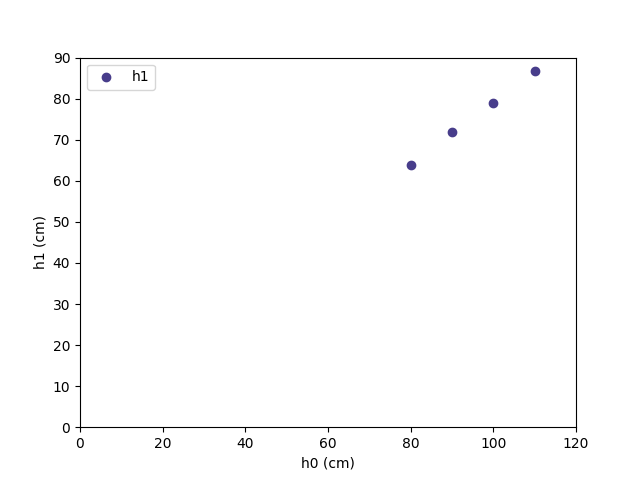
\includegraphics{Metodo1/computed_data/zoom_pallina4.png}
			} %close resize
		} %close centering
	\caption{Figura9: \(h1_{(h_{0})}\) - pallina da golf su marmo}
	\end{figure}
	
	\noindent Utilizzando il metodo dei minimi quadrati pesati abbiamo calcolato il coefficiente angolare e l'intercetta della retta:\\
	\[ con\quad\Delta = N(\sum \frac{x_{i}^{2}}{\sigma _{y_{i}}^{2}})-(\sum \frac{x_{i}}{\sigma _{y_{i}}^{2}})^{2}\]\\
	\[B = \frac{N(\sum\frac{x_{i}y_{i}}{\sigma _{y_{i}}^{2}})-\sum\frac{x_{i}}{\sigma _{y_{i}}^{2}}\sum\frac{y_{i}}{\sigma _{y_{i}}^{2}}}{\Delta } \quad
	\sigma _{B} = \sqrt{\frac{\sum \frac{1}{\sigma _{y_{i}}^{2}}}{\Delta}} \qquad
	\Rightarrow \qquad B = 0.761 \pm 0.008\]\\
	\[A = \frac{\sum \frac{(x_{i})^{2}}{\sigma _{y_{i}}^{2}}\sum \frac{(y_{i})^{2}}{\sigma _{y_{i}}^{2}}-\sum \frac{x_{i}}{\sigma _{y_{i}}^{2}}\sum \frac{x_{i}y_{i}}{\sigma _{y_{i}}^{2}}}{\Delta} \quad  \sigma _{A} = \sqrt{\frac{\sum \frac{x^{2}}{\sigma _{y_{i}}^{2}}}{\Delta}} \qquad \Rightarrow \qquad A = 3.161 \pm 0.735\]\\
	
	%retta interpolata pallina 4
	\begin{figure}[!ht]
			\captionsetup{labelformat=empty}
		\makebox[1 \textwidth][c]{       %centering table
			\resizebox{0.61 \textwidth}{!}{   %resize table
				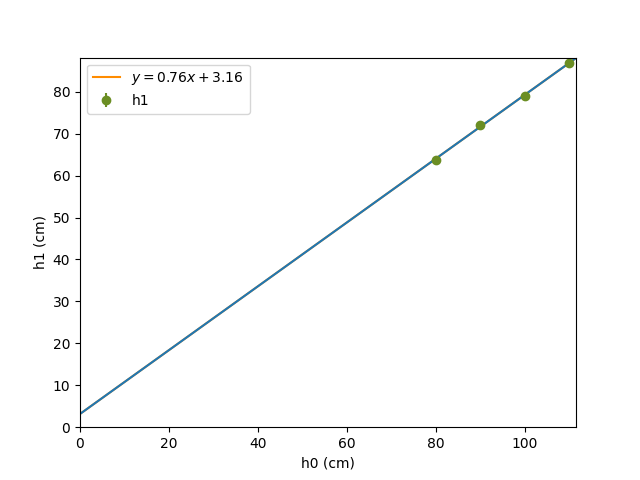
\includegraphics{Metodo1/computed_data/interpolazione_pallina4.png}
			} %close resize
		} %close centering
	\caption{Figura10: \(h1_{(h_{0})}\) - pallina da golf - interpolazione}
	\end{figure}
	
	\noindent Ricaviamo il coefficiente di restituzione
	
	\[ev = \sqrt{\frac{h_{1}}{h_{0}}} \rightarrow ev = \sqrt{B}\]
	
	\makebox[\textwidth]{
		{	
			\normalsize
			propagazione degli errori \(\rightarrow \quad  \sigma _{ev} = \frac{\sigma _{B}}{2\sqrt{B}} \)
		}
	}
	\[ev = 0.872 \pm 0.005\]
\noindent Test del chi quadro\\
\[\chi ^{2} = \sum \left ( \frac{y_{i}-A-BX_{i}}{\sigma_{i}} \right )^{2} = 0.931\]
\noindent considerando 1 grado di libertà \(\rightarrow \)  possiamo considerare l'ipotesi vera, con una sicurezza del 32 \(\%\).\\
L'attrito dell'aria non ha influenzato notevolmente il fenomeno; considerando infatti \(h_{lim} = 110 cm\)
\[\frac{F_{attrito \quad aereo}}{F_{peso}} = 0.018\]
con una massa di 0.0415Kg ed un diametro di 0.042 metri, abbiamo perso solo l'1,8\(\%\) dell'accelerazione data dalla gravità.
	\subsubsection*{metodo 2}
	%metodo due pallina 4
	gli intervalli misurati da 80cm in secondi:
	\begin{figure}[!h]
		\makebox[1 \textwidth][c]{
			\begin{tabular}{c|*{7}{c}}
				numero rimbalzo & lancio1 & lancio2 & lancio3 & lancio4 & lancio5 & media\\
				\hline
				1 & 0.649 & 0.723 & 0.724 & 0.722 & 0.723 &\(	0.708\pm0.015 \) \\
				\hline
				2 & 0.584 & 0.642 & 0.649 & 0.647 & 0.649 &\( 0.634\pm 0.013\)  \\
				\hline
				3 & 0.523 & 0.577 & 0.588 & 0.584 & 0.576 & \( 0.5610\pm 0.012\) \\
				\hline
				4 & 0.523 & 0.518 & 0.532 & 0.525 & 0.513 &\( 0.522 \pm 0.003\) \\
				\hline
				5 & 0.464 & 0.469 & 0.479 & 0.471 & 0.459 &\(0.468\pm 0.003\)  \\
				\hline
				6 & 0.407 & 0.422 & 0.436 & 0.421 & 0.411 &\( 0.411\pm0.005\) \\
				\hline
				7 & 0.364 & 0.384 & 0.391 & 0.376 & 0.366 & \(0.376\pm0.005\)\\
				\hline
				8 & 0.328 & 0.349 & 0.350 & 0.337 & 0.326 &\( 0.338\pm0.005\) \\
				\hline
			\end{tabular}
		} 
	\end{figure}
	.\\\\\\\\\\\\\\\\\\\\\\\\\\\\\\\\\\
	\noindent gli intervalli misurati da 90cm in secondi:

	\begin{figure}[!h]
		\makebox[1 \textwidth][c]{
			\begin{tabular}{c|*{7}{c}}
				numero rimbalzo & lancio1 & lancio2 & lancio3 & lancio4 & lancio5 & media\\
				\hline
				1 & 0.675 & 0.762 & 0.759 & 0.764 & 0.763 & \(0.745 \pm0.017\)\\
				\hline
				2 & 0.604 & 0.682 & 0.680 & 0.683 & 0.683 &\(  0.666\pm0.016\)\\
				\hline
				3 & 0.533 & 0.612 & 0.606 & 0.609 & 0.614 &\( 0.595\pm0.016\)\\
				\hline
				4 & 0.478 & 0.551 & 0.544 & 0.545 & 0.558 &\(  0.535 \pm0.014\) \\
				\hline
				5 & 0.432 & 0.494 & 0.489 & 0.479 & 0.505 &\( 0.480\pm0.013\)\\
				\hline
				6 & 0.386 & 0.439 & 0.437 & 0.426 & 0.458 & \(  0.429\pm0.012\)\\
				\hline
				7 & 0.349 & 0.391 & 0.388 & 0.378 & 0.416 &\(0.3847\pm0011\) \\
				\hline
				8 & 0.316 & 0.345 & 0.349 & 0.338 & 0.378 &\( 0.345\pm0.010\) \\
				\hline
			\end{tabular}
		} 
	\end{figure}
	
\noindent 	gli intervalli misurati da 100cm in secondi:
	\begin{figure}[!h]
		\makebox[1 \textwidth][c]{
			\begin{tabular}{c|*{7}{c}}
				numero rimbalzo & lancio1 & lancio2 & lancio3 & lancio4 & lancio5 & media\\
				\hline
				1 & 0.794 & 0.811 & 0.804 & 0.791 & 0.804 &\(0.801 \pm0.004\) \\
				\hline
				2 & 0.716 & 0.725 & 0.718 & 0.710 & 0.716 &\(    0.7172 \pm0.0024\) \\
				\hline
				3 & 0.637 & 0.643 & 0.644 & 0.638 & 0.645 &\( 0.6414\pm0.0017\) \\
				\hline
				4 & 0.562 & 0.580 & 0.580 & 0.574 & 0.581 &\( 0.575\pm0.004\) \\
				\hline
				5 & 0.504 & 0.518 & 0.501 & 0.518 & 0.525 & \( 0.513\pm0.005\)\\
				\hline
				6 & 0.452 & 0.460 & 0.450 & 0.468 & 0.473 &\(  0.461\pm 0.005\) \\
				\hline
				7 & 0.403 & 0.421 & 0.401 & 0.425 & 0.429 &\(0.416\pm0.006\) \\
				\hline
				8 & 0.367 & 0.359 & 0.356 & 0.386 & 0.391 & \( 0.372\pm0.007\)\\
				\hline
			\end{tabular}
		} 
	\end{figure}

	\noindent gli intervalli misurati da 110cm in secondi:
	\begin{figure}[!h]
		\makebox[1 \textwidth][c]{
			\begin{tabular}{c|*{7}{c}}
				numero rimbalzo & lancio1 & lancio2 & lancio3 & lancio4 & lancio5 & media\\
				\hline
				1 & 0.845 & 0.838 & 0.838 & 0.832 & 0.845 &\(	0.8396\pm 0.0025\) \\
				\hline
				2 & 0.760 & 0.751 & 0.746 & 0.742 & 0.753 &\(0.750\pm 0.003\) \\
				\hline
				3 & 0.682 & 0.673 & 0.666 & 0.665 & 0.675 &\(     0.672\pm0.003\) \\
				\hline
				4 & 0.608 & 0.607 & 0.594 & 0.591 & 0.609 &\( 0.602 \pm 0.004\) \\
				\hline
				5 & 0.543 & 0.547 & 0.528 & 0.527 & 0.549 & \( 0.539 \pm 0.005\)\\
				\hline
				6 & 0.488 & 0.492 & 0.465 & 0.472 & 0.493 &\( 0.482\pm0.006\) \\
				\hline
				7 & 0.421 & 0.438 & 0.417 & 0.423 & 0.441 &\(	0.428\pm 0.005\) \\
				\hline
				8 & 0.377 & 0.388 & 0.372 & 0.365 & 0.396 & \( 0.380 \pm 0.006\)\\
				\hline
			\end{tabular}
		} 
	\end{figure}
.\\\\\\\\\\\\\\\\\\\\\\	
	\begin{figure}[!ht]
		\makebox[1 \textwidth][c]{       %centering table
			\resizebox{0.7 \textwidth}{!}{   %resize table
				%%% Creator: Matplotlib, PGF backend
%%
%% To include the figure in your LaTeX document, write
%%   \input{<filename>.pgf}
%%
%% Make sure the required packages are loaded in your preamble
%%   \usepackage{pgf}
%%
%% and, on pdftex
%%   \usepackage[utf8]{inputenc}\DeclareUnicodeCharacter{2212}{-}
%%
%% or, on luatex and xetex
%%   \usepackage{unicode-math}
%%
%% Figures using additional raster images can only be included by \input if
%% they are in the same directory as the main LaTeX file. For loading figures
%% from other directories you can use the `import` package
%%   \usepackage{import}
%%
%% and then include the figures with
%%   \import{<path to file>}{<filename>.pgf}
%%
%% Matplotlib used the following preamble
%%   \usepackage{fontspec}
%%   \setmainfont{DejaVuSerif.ttf}[Path=C:/Users/giuly/AppData/Local/Programs/Python/Python39/Lib/site-packages/matplotlib/mpl-data/fonts/ttf/]
%%   \setsansfont{DejaVuSans.ttf}[Path=C:/Users/giuly/AppData/Local/Programs/Python/Python39/Lib/site-packages/matplotlib/mpl-data/fonts/ttf/]
%%   \setmonofont{DejaVuSansMono.ttf}[Path=C:/Users/giuly/AppData/Local/Programs/Python/Python39/Lib/site-packages/matplotlib/mpl-data/fonts/ttf/]
%%
\begingroup%
\makeatletter%
\begin{pgfpicture}%
\pgfpathrectangle{\pgfpointorigin}{\pgfqpoint{6.400000in}{4.800000in}}%
\pgfusepath{use as bounding box, clip}%
\begin{pgfscope}%
\pgfsetbuttcap%
\pgfsetmiterjoin%
\definecolor{currentfill}{rgb}{1.000000,1.000000,1.000000}%
\pgfsetfillcolor{currentfill}%
\pgfsetlinewidth{0.000000pt}%
\definecolor{currentstroke}{rgb}{1.000000,1.000000,1.000000}%
\pgfsetstrokecolor{currentstroke}%
\pgfsetdash{}{0pt}%
\pgfpathmoveto{\pgfqpoint{0.000000in}{0.000000in}}%
\pgfpathlineto{\pgfqpoint{6.400000in}{0.000000in}}%
\pgfpathlineto{\pgfqpoint{6.400000in}{4.800000in}}%
\pgfpathlineto{\pgfqpoint{0.000000in}{4.800000in}}%
\pgfpathclose%
\pgfusepath{fill}%
\end{pgfscope}%
\begin{pgfscope}%
\pgfsetbuttcap%
\pgfsetmiterjoin%
\definecolor{currentfill}{rgb}{1.000000,1.000000,1.000000}%
\pgfsetfillcolor{currentfill}%
\pgfsetlinewidth{0.000000pt}%
\definecolor{currentstroke}{rgb}{0.000000,0.000000,0.000000}%
\pgfsetstrokecolor{currentstroke}%
\pgfsetstrokeopacity{0.000000}%
\pgfsetdash{}{0pt}%
\pgfpathmoveto{\pgfqpoint{0.800000in}{0.528000in}}%
\pgfpathlineto{\pgfqpoint{5.760000in}{0.528000in}}%
\pgfpathlineto{\pgfqpoint{5.760000in}{4.224000in}}%
\pgfpathlineto{\pgfqpoint{0.800000in}{4.224000in}}%
\pgfpathclose%
\pgfusepath{fill}%
\end{pgfscope}%
\begin{pgfscope}%
\pgfpathrectangle{\pgfqpoint{0.800000in}{0.528000in}}{\pgfqpoint{4.960000in}{3.696000in}}%
\pgfusepath{clip}%
\pgfsetbuttcap%
\pgfsetmiterjoin%
\definecolor{currentfill}{rgb}{0.400000,0.803922,0.666667}%
\pgfsetfillcolor{currentfill}%
\pgfsetfillopacity{0.800000}%
\pgfsetlinewidth{0.000000pt}%
\definecolor{currentstroke}{rgb}{0.000000,0.000000,0.000000}%
\pgfsetstrokecolor{currentstroke}%
\pgfsetstrokeopacity{0.800000}%
\pgfsetdash{}{0pt}%
\pgfpathmoveto{\pgfqpoint{1.025455in}{0.528000in}}%
\pgfpathlineto{\pgfqpoint{1.401212in}{0.528000in}}%
\pgfpathlineto{\pgfqpoint{1.401212in}{0.848000in}}%
\pgfpathlineto{\pgfqpoint{1.025455in}{0.848000in}}%
\pgfpathclose%
\pgfusepath{fill}%
\end{pgfscope}%
\begin{pgfscope}%
\pgfpathrectangle{\pgfqpoint{0.800000in}{0.528000in}}{\pgfqpoint{4.960000in}{3.696000in}}%
\pgfusepath{clip}%
\pgfsetbuttcap%
\pgfsetmiterjoin%
\definecolor{currentfill}{rgb}{0.400000,0.803922,0.666667}%
\pgfsetfillcolor{currentfill}%
\pgfsetfillopacity{0.800000}%
\pgfsetlinewidth{0.000000pt}%
\definecolor{currentstroke}{rgb}{0.000000,0.000000,0.000000}%
\pgfsetstrokecolor{currentstroke}%
\pgfsetstrokeopacity{0.800000}%
\pgfsetdash{}{0pt}%
\pgfpathmoveto{\pgfqpoint{1.401212in}{0.528000in}}%
\pgfpathlineto{\pgfqpoint{1.776970in}{0.528000in}}%
\pgfpathlineto{\pgfqpoint{1.776970in}{0.848000in}}%
\pgfpathlineto{\pgfqpoint{1.401212in}{0.848000in}}%
\pgfpathclose%
\pgfusepath{fill}%
\end{pgfscope}%
\begin{pgfscope}%
\pgfpathrectangle{\pgfqpoint{0.800000in}{0.528000in}}{\pgfqpoint{4.960000in}{3.696000in}}%
\pgfusepath{clip}%
\pgfsetbuttcap%
\pgfsetmiterjoin%
\definecolor{currentfill}{rgb}{0.400000,0.803922,0.666667}%
\pgfsetfillcolor{currentfill}%
\pgfsetfillopacity{0.800000}%
\pgfsetlinewidth{0.000000pt}%
\definecolor{currentstroke}{rgb}{0.000000,0.000000,0.000000}%
\pgfsetstrokecolor{currentstroke}%
\pgfsetstrokeopacity{0.800000}%
\pgfsetdash{}{0pt}%
\pgfpathmoveto{\pgfqpoint{1.776970in}{0.528000in}}%
\pgfpathlineto{\pgfqpoint{2.152727in}{0.528000in}}%
\pgfpathlineto{\pgfqpoint{2.152727in}{1.168000in}}%
\pgfpathlineto{\pgfqpoint{1.776970in}{1.168000in}}%
\pgfpathclose%
\pgfusepath{fill}%
\end{pgfscope}%
\begin{pgfscope}%
\pgfpathrectangle{\pgfqpoint{0.800000in}{0.528000in}}{\pgfqpoint{4.960000in}{3.696000in}}%
\pgfusepath{clip}%
\pgfsetbuttcap%
\pgfsetmiterjoin%
\definecolor{currentfill}{rgb}{0.400000,0.803922,0.666667}%
\pgfsetfillcolor{currentfill}%
\pgfsetfillopacity{0.800000}%
\pgfsetlinewidth{0.000000pt}%
\definecolor{currentstroke}{rgb}{0.000000,0.000000,0.000000}%
\pgfsetstrokecolor{currentstroke}%
\pgfsetstrokeopacity{0.800000}%
\pgfsetdash{}{0pt}%
\pgfpathmoveto{\pgfqpoint{2.152727in}{0.528000in}}%
\pgfpathlineto{\pgfqpoint{2.528485in}{0.528000in}}%
\pgfpathlineto{\pgfqpoint{2.528485in}{1.968000in}}%
\pgfpathlineto{\pgfqpoint{2.152727in}{1.968000in}}%
\pgfpathclose%
\pgfusepath{fill}%
\end{pgfscope}%
\begin{pgfscope}%
\pgfpathrectangle{\pgfqpoint{0.800000in}{0.528000in}}{\pgfqpoint{4.960000in}{3.696000in}}%
\pgfusepath{clip}%
\pgfsetbuttcap%
\pgfsetmiterjoin%
\definecolor{currentfill}{rgb}{0.400000,0.803922,0.666667}%
\pgfsetfillcolor{currentfill}%
\pgfsetfillopacity{0.800000}%
\pgfsetlinewidth{0.000000pt}%
\definecolor{currentstroke}{rgb}{0.000000,0.000000,0.000000}%
\pgfsetstrokecolor{currentstroke}%
\pgfsetstrokeopacity{0.800000}%
\pgfsetdash{}{0pt}%
\pgfpathmoveto{\pgfqpoint{2.528485in}{0.528000in}}%
\pgfpathlineto{\pgfqpoint{2.904242in}{0.528000in}}%
\pgfpathlineto{\pgfqpoint{2.904242in}{2.448000in}}%
\pgfpathlineto{\pgfqpoint{2.528485in}{2.448000in}}%
\pgfpathclose%
\pgfusepath{fill}%
\end{pgfscope}%
\begin{pgfscope}%
\pgfpathrectangle{\pgfqpoint{0.800000in}{0.528000in}}{\pgfqpoint{4.960000in}{3.696000in}}%
\pgfusepath{clip}%
\pgfsetbuttcap%
\pgfsetmiterjoin%
\definecolor{currentfill}{rgb}{0.400000,0.803922,0.666667}%
\pgfsetfillcolor{currentfill}%
\pgfsetfillopacity{0.800000}%
\pgfsetlinewidth{0.000000pt}%
\definecolor{currentstroke}{rgb}{0.000000,0.000000,0.000000}%
\pgfsetstrokecolor{currentstroke}%
\pgfsetstrokeopacity{0.800000}%
\pgfsetdash{}{0pt}%
\pgfpathmoveto{\pgfqpoint{2.904242in}{0.528000in}}%
\pgfpathlineto{\pgfqpoint{3.280000in}{0.528000in}}%
\pgfpathlineto{\pgfqpoint{3.280000in}{4.048000in}}%
\pgfpathlineto{\pgfqpoint{2.904242in}{4.048000in}}%
\pgfpathclose%
\pgfusepath{fill}%
\end{pgfscope}%
\begin{pgfscope}%
\pgfpathrectangle{\pgfqpoint{0.800000in}{0.528000in}}{\pgfqpoint{4.960000in}{3.696000in}}%
\pgfusepath{clip}%
\pgfsetbuttcap%
\pgfsetmiterjoin%
\definecolor{currentfill}{rgb}{0.400000,0.803922,0.666667}%
\pgfsetfillcolor{currentfill}%
\pgfsetfillopacity{0.800000}%
\pgfsetlinewidth{0.000000pt}%
\definecolor{currentstroke}{rgb}{0.000000,0.000000,0.000000}%
\pgfsetstrokecolor{currentstroke}%
\pgfsetstrokeopacity{0.800000}%
\pgfsetdash{}{0pt}%
\pgfpathmoveto{\pgfqpoint{3.280000in}{0.528000in}}%
\pgfpathlineto{\pgfqpoint{3.655758in}{0.528000in}}%
\pgfpathlineto{\pgfqpoint{3.655758in}{3.248000in}}%
\pgfpathlineto{\pgfqpoint{3.280000in}{3.248000in}}%
\pgfpathclose%
\pgfusepath{fill}%
\end{pgfscope}%
\begin{pgfscope}%
\pgfpathrectangle{\pgfqpoint{0.800000in}{0.528000in}}{\pgfqpoint{4.960000in}{3.696000in}}%
\pgfusepath{clip}%
\pgfsetbuttcap%
\pgfsetmiterjoin%
\definecolor{currentfill}{rgb}{0.400000,0.803922,0.666667}%
\pgfsetfillcolor{currentfill}%
\pgfsetfillopacity{0.800000}%
\pgfsetlinewidth{0.000000pt}%
\definecolor{currentstroke}{rgb}{0.000000,0.000000,0.000000}%
\pgfsetstrokecolor{currentstroke}%
\pgfsetstrokeopacity{0.800000}%
\pgfsetdash{}{0pt}%
\pgfpathmoveto{\pgfqpoint{3.655758in}{0.528000in}}%
\pgfpathlineto{\pgfqpoint{4.031515in}{0.528000in}}%
\pgfpathlineto{\pgfqpoint{4.031515in}{3.248000in}}%
\pgfpathlineto{\pgfqpoint{3.655758in}{3.248000in}}%
\pgfpathclose%
\pgfusepath{fill}%
\end{pgfscope}%
\begin{pgfscope}%
\pgfpathrectangle{\pgfqpoint{0.800000in}{0.528000in}}{\pgfqpoint{4.960000in}{3.696000in}}%
\pgfusepath{clip}%
\pgfsetbuttcap%
\pgfsetmiterjoin%
\definecolor{currentfill}{rgb}{0.400000,0.803922,0.666667}%
\pgfsetfillcolor{currentfill}%
\pgfsetfillopacity{0.800000}%
\pgfsetlinewidth{0.000000pt}%
\definecolor{currentstroke}{rgb}{0.000000,0.000000,0.000000}%
\pgfsetstrokecolor{currentstroke}%
\pgfsetstrokeopacity{0.800000}%
\pgfsetdash{}{0pt}%
\pgfpathmoveto{\pgfqpoint{4.031515in}{0.528000in}}%
\pgfpathlineto{\pgfqpoint{4.407273in}{0.528000in}}%
\pgfpathlineto{\pgfqpoint{4.407273in}{1.968000in}}%
\pgfpathlineto{\pgfqpoint{4.031515in}{1.968000in}}%
\pgfpathclose%
\pgfusepath{fill}%
\end{pgfscope}%
\begin{pgfscope}%
\pgfpathrectangle{\pgfqpoint{0.800000in}{0.528000in}}{\pgfqpoint{4.960000in}{3.696000in}}%
\pgfusepath{clip}%
\pgfsetbuttcap%
\pgfsetmiterjoin%
\definecolor{currentfill}{rgb}{0.400000,0.803922,0.666667}%
\pgfsetfillcolor{currentfill}%
\pgfsetfillopacity{0.800000}%
\pgfsetlinewidth{0.000000pt}%
\definecolor{currentstroke}{rgb}{0.000000,0.000000,0.000000}%
\pgfsetstrokecolor{currentstroke}%
\pgfsetstrokeopacity{0.800000}%
\pgfsetdash{}{0pt}%
\pgfpathmoveto{\pgfqpoint{4.407273in}{0.528000in}}%
\pgfpathlineto{\pgfqpoint{4.783030in}{0.528000in}}%
\pgfpathlineto{\pgfqpoint{4.783030in}{1.168000in}}%
\pgfpathlineto{\pgfqpoint{4.407273in}{1.168000in}}%
\pgfpathclose%
\pgfusepath{fill}%
\end{pgfscope}%
\begin{pgfscope}%
\pgfpathrectangle{\pgfqpoint{0.800000in}{0.528000in}}{\pgfqpoint{4.960000in}{3.696000in}}%
\pgfusepath{clip}%
\pgfsetbuttcap%
\pgfsetmiterjoin%
\definecolor{currentfill}{rgb}{0.400000,0.803922,0.666667}%
\pgfsetfillcolor{currentfill}%
\pgfsetfillopacity{0.800000}%
\pgfsetlinewidth{0.000000pt}%
\definecolor{currentstroke}{rgb}{0.000000,0.000000,0.000000}%
\pgfsetstrokecolor{currentstroke}%
\pgfsetstrokeopacity{0.800000}%
\pgfsetdash{}{0pt}%
\pgfpathmoveto{\pgfqpoint{4.783030in}{0.528000in}}%
\pgfpathlineto{\pgfqpoint{5.158788in}{0.528000in}}%
\pgfpathlineto{\pgfqpoint{5.158788in}{0.688000in}}%
\pgfpathlineto{\pgfqpoint{4.783030in}{0.688000in}}%
\pgfpathclose%
\pgfusepath{fill}%
\end{pgfscope}%
\begin{pgfscope}%
\pgfpathrectangle{\pgfqpoint{0.800000in}{0.528000in}}{\pgfqpoint{4.960000in}{3.696000in}}%
\pgfusepath{clip}%
\pgfsetbuttcap%
\pgfsetmiterjoin%
\definecolor{currentfill}{rgb}{0.400000,0.803922,0.666667}%
\pgfsetfillcolor{currentfill}%
\pgfsetfillopacity{0.800000}%
\pgfsetlinewidth{0.000000pt}%
\definecolor{currentstroke}{rgb}{0.000000,0.000000,0.000000}%
\pgfsetstrokecolor{currentstroke}%
\pgfsetstrokeopacity{0.800000}%
\pgfsetdash{}{0pt}%
\pgfpathmoveto{\pgfqpoint{5.158788in}{0.528000in}}%
\pgfpathlineto{\pgfqpoint{5.534545in}{0.528000in}}%
\pgfpathlineto{\pgfqpoint{5.534545in}{0.688000in}}%
\pgfpathlineto{\pgfqpoint{5.158788in}{0.688000in}}%
\pgfpathclose%
\pgfusepath{fill}%
\end{pgfscope}%
\begin{pgfscope}%
\pgfsetbuttcap%
\pgfsetroundjoin%
\definecolor{currentfill}{rgb}{0.000000,0.000000,0.000000}%
\pgfsetfillcolor{currentfill}%
\pgfsetlinewidth{0.803000pt}%
\definecolor{currentstroke}{rgb}{0.000000,0.000000,0.000000}%
\pgfsetstrokecolor{currentstroke}%
\pgfsetdash{}{0pt}%
\pgfsys@defobject{currentmarker}{\pgfqpoint{0.000000in}{-0.048611in}}{\pgfqpoint{0.000000in}{0.000000in}}{%
\pgfpathmoveto{\pgfqpoint{0.000000in}{0.000000in}}%
\pgfpathlineto{\pgfqpoint{0.000000in}{-0.048611in}}%
\pgfusepath{stroke,fill}%
}%
\begin{pgfscope}%
\pgfsys@transformshift{1.025455in}{0.528000in}%
\pgfsys@useobject{currentmarker}{}%
\end{pgfscope}%
\end{pgfscope}%
\begin{pgfscope}%
\definecolor{textcolor}{rgb}{0.000000,0.000000,0.000000}%
\pgfsetstrokecolor{textcolor}%
\pgfsetfillcolor{textcolor}%
\pgftext[x=1.025455in,y=0.430778in,,top]{\color{textcolor}\sffamily\fontsize{10.000000}{12.000000}\selectfont 1.30}%
\end{pgfscope}%
\begin{pgfscope}%
\pgfsetbuttcap%
\pgfsetroundjoin%
\definecolor{currentfill}{rgb}{0.000000,0.000000,0.000000}%
\pgfsetfillcolor{currentfill}%
\pgfsetlinewidth{0.803000pt}%
\definecolor{currentstroke}{rgb}{0.000000,0.000000,0.000000}%
\pgfsetstrokecolor{currentstroke}%
\pgfsetdash{}{0pt}%
\pgfsys@defobject{currentmarker}{\pgfqpoint{0.000000in}{-0.048611in}}{\pgfqpoint{0.000000in}{0.000000in}}{%
\pgfpathmoveto{\pgfqpoint{0.000000in}{0.000000in}}%
\pgfpathlineto{\pgfqpoint{0.000000in}{-0.048611in}}%
\pgfusepath{stroke,fill}%
}%
\begin{pgfscope}%
\pgfsys@transformshift{1.589091in}{0.528000in}%
\pgfsys@useobject{currentmarker}{}%
\end{pgfscope}%
\end{pgfscope}%
\begin{pgfscope}%
\definecolor{textcolor}{rgb}{0.000000,0.000000,0.000000}%
\pgfsetstrokecolor{textcolor}%
\pgfsetfillcolor{textcolor}%
\pgftext[x=1.589091in,y=0.430778in,,top]{\color{textcolor}\sffamily\fontsize{10.000000}{12.000000}\selectfont 1.35}%
\end{pgfscope}%
\begin{pgfscope}%
\pgfsetbuttcap%
\pgfsetroundjoin%
\definecolor{currentfill}{rgb}{0.000000,0.000000,0.000000}%
\pgfsetfillcolor{currentfill}%
\pgfsetlinewidth{0.803000pt}%
\definecolor{currentstroke}{rgb}{0.000000,0.000000,0.000000}%
\pgfsetstrokecolor{currentstroke}%
\pgfsetdash{}{0pt}%
\pgfsys@defobject{currentmarker}{\pgfqpoint{0.000000in}{-0.048611in}}{\pgfqpoint{0.000000in}{0.000000in}}{%
\pgfpathmoveto{\pgfqpoint{0.000000in}{0.000000in}}%
\pgfpathlineto{\pgfqpoint{0.000000in}{-0.048611in}}%
\pgfusepath{stroke,fill}%
}%
\begin{pgfscope}%
\pgfsys@transformshift{2.152727in}{0.528000in}%
\pgfsys@useobject{currentmarker}{}%
\end{pgfscope}%
\end{pgfscope}%
\begin{pgfscope}%
\definecolor{textcolor}{rgb}{0.000000,0.000000,0.000000}%
\pgfsetstrokecolor{textcolor}%
\pgfsetfillcolor{textcolor}%
\pgftext[x=2.152727in,y=0.430778in,,top]{\color{textcolor}\sffamily\fontsize{10.000000}{12.000000}\selectfont 1.40}%
\end{pgfscope}%
\begin{pgfscope}%
\pgfsetbuttcap%
\pgfsetroundjoin%
\definecolor{currentfill}{rgb}{0.000000,0.000000,0.000000}%
\pgfsetfillcolor{currentfill}%
\pgfsetlinewidth{0.803000pt}%
\definecolor{currentstroke}{rgb}{0.000000,0.000000,0.000000}%
\pgfsetstrokecolor{currentstroke}%
\pgfsetdash{}{0pt}%
\pgfsys@defobject{currentmarker}{\pgfqpoint{0.000000in}{-0.048611in}}{\pgfqpoint{0.000000in}{0.000000in}}{%
\pgfpathmoveto{\pgfqpoint{0.000000in}{0.000000in}}%
\pgfpathlineto{\pgfqpoint{0.000000in}{-0.048611in}}%
\pgfusepath{stroke,fill}%
}%
\begin{pgfscope}%
\pgfsys@transformshift{2.716364in}{0.528000in}%
\pgfsys@useobject{currentmarker}{}%
\end{pgfscope}%
\end{pgfscope}%
\begin{pgfscope}%
\definecolor{textcolor}{rgb}{0.000000,0.000000,0.000000}%
\pgfsetstrokecolor{textcolor}%
\pgfsetfillcolor{textcolor}%
\pgftext[x=2.716364in,y=0.430778in,,top]{\color{textcolor}\sffamily\fontsize{10.000000}{12.000000}\selectfont 1.45}%
\end{pgfscope}%
\begin{pgfscope}%
\pgfsetbuttcap%
\pgfsetroundjoin%
\definecolor{currentfill}{rgb}{0.000000,0.000000,0.000000}%
\pgfsetfillcolor{currentfill}%
\pgfsetlinewidth{0.803000pt}%
\definecolor{currentstroke}{rgb}{0.000000,0.000000,0.000000}%
\pgfsetstrokecolor{currentstroke}%
\pgfsetdash{}{0pt}%
\pgfsys@defobject{currentmarker}{\pgfqpoint{0.000000in}{-0.048611in}}{\pgfqpoint{0.000000in}{0.000000in}}{%
\pgfpathmoveto{\pgfqpoint{0.000000in}{0.000000in}}%
\pgfpathlineto{\pgfqpoint{0.000000in}{-0.048611in}}%
\pgfusepath{stroke,fill}%
}%
\begin{pgfscope}%
\pgfsys@transformshift{3.280000in}{0.528000in}%
\pgfsys@useobject{currentmarker}{}%
\end{pgfscope}%
\end{pgfscope}%
\begin{pgfscope}%
\definecolor{textcolor}{rgb}{0.000000,0.000000,0.000000}%
\pgfsetstrokecolor{textcolor}%
\pgfsetfillcolor{textcolor}%
\pgftext[x=3.280000in,y=0.430778in,,top]{\color{textcolor}\sffamily\fontsize{10.000000}{12.000000}\selectfont 1.50}%
\end{pgfscope}%
\begin{pgfscope}%
\pgfsetbuttcap%
\pgfsetroundjoin%
\definecolor{currentfill}{rgb}{0.000000,0.000000,0.000000}%
\pgfsetfillcolor{currentfill}%
\pgfsetlinewidth{0.803000pt}%
\definecolor{currentstroke}{rgb}{0.000000,0.000000,0.000000}%
\pgfsetstrokecolor{currentstroke}%
\pgfsetdash{}{0pt}%
\pgfsys@defobject{currentmarker}{\pgfqpoint{0.000000in}{-0.048611in}}{\pgfqpoint{0.000000in}{0.000000in}}{%
\pgfpathmoveto{\pgfqpoint{0.000000in}{0.000000in}}%
\pgfpathlineto{\pgfqpoint{0.000000in}{-0.048611in}}%
\pgfusepath{stroke,fill}%
}%
\begin{pgfscope}%
\pgfsys@transformshift{3.843636in}{0.528000in}%
\pgfsys@useobject{currentmarker}{}%
\end{pgfscope}%
\end{pgfscope}%
\begin{pgfscope}%
\definecolor{textcolor}{rgb}{0.000000,0.000000,0.000000}%
\pgfsetstrokecolor{textcolor}%
\pgfsetfillcolor{textcolor}%
\pgftext[x=3.843636in,y=0.430778in,,top]{\color{textcolor}\sffamily\fontsize{10.000000}{12.000000}\selectfont 1.55}%
\end{pgfscope}%
\begin{pgfscope}%
\pgfsetbuttcap%
\pgfsetroundjoin%
\definecolor{currentfill}{rgb}{0.000000,0.000000,0.000000}%
\pgfsetfillcolor{currentfill}%
\pgfsetlinewidth{0.803000pt}%
\definecolor{currentstroke}{rgb}{0.000000,0.000000,0.000000}%
\pgfsetstrokecolor{currentstroke}%
\pgfsetdash{}{0pt}%
\pgfsys@defobject{currentmarker}{\pgfqpoint{0.000000in}{-0.048611in}}{\pgfqpoint{0.000000in}{0.000000in}}{%
\pgfpathmoveto{\pgfqpoint{0.000000in}{0.000000in}}%
\pgfpathlineto{\pgfqpoint{0.000000in}{-0.048611in}}%
\pgfusepath{stroke,fill}%
}%
\begin{pgfscope}%
\pgfsys@transformshift{4.407273in}{0.528000in}%
\pgfsys@useobject{currentmarker}{}%
\end{pgfscope}%
\end{pgfscope}%
\begin{pgfscope}%
\definecolor{textcolor}{rgb}{0.000000,0.000000,0.000000}%
\pgfsetstrokecolor{textcolor}%
\pgfsetfillcolor{textcolor}%
\pgftext[x=4.407273in,y=0.430778in,,top]{\color{textcolor}\sffamily\fontsize{10.000000}{12.000000}\selectfont 1.60}%
\end{pgfscope}%
\begin{pgfscope}%
\pgfsetbuttcap%
\pgfsetroundjoin%
\definecolor{currentfill}{rgb}{0.000000,0.000000,0.000000}%
\pgfsetfillcolor{currentfill}%
\pgfsetlinewidth{0.803000pt}%
\definecolor{currentstroke}{rgb}{0.000000,0.000000,0.000000}%
\pgfsetstrokecolor{currentstroke}%
\pgfsetdash{}{0pt}%
\pgfsys@defobject{currentmarker}{\pgfqpoint{0.000000in}{-0.048611in}}{\pgfqpoint{0.000000in}{0.000000in}}{%
\pgfpathmoveto{\pgfqpoint{0.000000in}{0.000000in}}%
\pgfpathlineto{\pgfqpoint{0.000000in}{-0.048611in}}%
\pgfusepath{stroke,fill}%
}%
\begin{pgfscope}%
\pgfsys@transformshift{4.970909in}{0.528000in}%
\pgfsys@useobject{currentmarker}{}%
\end{pgfscope}%
\end{pgfscope}%
\begin{pgfscope}%
\definecolor{textcolor}{rgb}{0.000000,0.000000,0.000000}%
\pgfsetstrokecolor{textcolor}%
\pgfsetfillcolor{textcolor}%
\pgftext[x=4.970909in,y=0.430778in,,top]{\color{textcolor}\sffamily\fontsize{10.000000}{12.000000}\selectfont 1.65}%
\end{pgfscope}%
\begin{pgfscope}%
\pgfsetbuttcap%
\pgfsetroundjoin%
\definecolor{currentfill}{rgb}{0.000000,0.000000,0.000000}%
\pgfsetfillcolor{currentfill}%
\pgfsetlinewidth{0.803000pt}%
\definecolor{currentstroke}{rgb}{0.000000,0.000000,0.000000}%
\pgfsetstrokecolor{currentstroke}%
\pgfsetdash{}{0pt}%
\pgfsys@defobject{currentmarker}{\pgfqpoint{0.000000in}{-0.048611in}}{\pgfqpoint{0.000000in}{0.000000in}}{%
\pgfpathmoveto{\pgfqpoint{0.000000in}{0.000000in}}%
\pgfpathlineto{\pgfqpoint{0.000000in}{-0.048611in}}%
\pgfusepath{stroke,fill}%
}%
\begin{pgfscope}%
\pgfsys@transformshift{5.534545in}{0.528000in}%
\pgfsys@useobject{currentmarker}{}%
\end{pgfscope}%
\end{pgfscope}%
\begin{pgfscope}%
\definecolor{textcolor}{rgb}{0.000000,0.000000,0.000000}%
\pgfsetstrokecolor{textcolor}%
\pgfsetfillcolor{textcolor}%
\pgftext[x=5.534545in,y=0.430778in,,top]{\color{textcolor}\sffamily\fontsize{10.000000}{12.000000}\selectfont 1.70}%
\end{pgfscope}%
\begin{pgfscope}%
\definecolor{textcolor}{rgb}{0.000000,0.000000,0.000000}%
\pgfsetstrokecolor{textcolor}%
\pgfsetfillcolor{textcolor}%
\pgftext[x=3.280000in,y=0.240809in,,top]{\color{textcolor}\sffamily\fontsize{10.000000}{12.000000}\selectfont \(\displaystyle x_k\) (s)}%
\end{pgfscope}%
\begin{pgfscope}%
\pgfsetbuttcap%
\pgfsetroundjoin%
\definecolor{currentfill}{rgb}{0.000000,0.000000,0.000000}%
\pgfsetfillcolor{currentfill}%
\pgfsetlinewidth{0.803000pt}%
\definecolor{currentstroke}{rgb}{0.000000,0.000000,0.000000}%
\pgfsetstrokecolor{currentstroke}%
\pgfsetdash{}{0pt}%
\pgfsys@defobject{currentmarker}{\pgfqpoint{-0.048611in}{0.000000in}}{\pgfqpoint{-0.000000in}{0.000000in}}{%
\pgfpathmoveto{\pgfqpoint{-0.000000in}{0.000000in}}%
\pgfpathlineto{\pgfqpoint{-0.048611in}{0.000000in}}%
\pgfusepath{stroke,fill}%
}%
\begin{pgfscope}%
\pgfsys@transformshift{0.800000in}{0.528000in}%
\pgfsys@useobject{currentmarker}{}%
\end{pgfscope}%
\end{pgfscope}%
\begin{pgfscope}%
\definecolor{textcolor}{rgb}{0.000000,0.000000,0.000000}%
\pgfsetstrokecolor{textcolor}%
\pgfsetfillcolor{textcolor}%
\pgftext[x=0.614412in, y=0.475238in, left, base]{\color{textcolor}\sffamily\fontsize{10.000000}{12.000000}\selectfont 0}%
\end{pgfscope}%
\begin{pgfscope}%
\pgfsetbuttcap%
\pgfsetroundjoin%
\definecolor{currentfill}{rgb}{0.000000,0.000000,0.000000}%
\pgfsetfillcolor{currentfill}%
\pgfsetlinewidth{0.803000pt}%
\definecolor{currentstroke}{rgb}{0.000000,0.000000,0.000000}%
\pgfsetstrokecolor{currentstroke}%
\pgfsetdash{}{0pt}%
\pgfsys@defobject{currentmarker}{\pgfqpoint{-0.048611in}{0.000000in}}{\pgfqpoint{-0.000000in}{0.000000in}}{%
\pgfpathmoveto{\pgfqpoint{-0.000000in}{0.000000in}}%
\pgfpathlineto{\pgfqpoint{-0.048611in}{0.000000in}}%
\pgfusepath{stroke,fill}%
}%
\begin{pgfscope}%
\pgfsys@transformshift{0.800000in}{1.061333in}%
\pgfsys@useobject{currentmarker}{}%
\end{pgfscope}%
\end{pgfscope}%
\begin{pgfscope}%
\definecolor{textcolor}{rgb}{0.000000,0.000000,0.000000}%
\pgfsetstrokecolor{textcolor}%
\pgfsetfillcolor{textcolor}%
\pgftext[x=0.614412in, y=1.008572in, left, base]{\color{textcolor}\sffamily\fontsize{10.000000}{12.000000}\selectfont 1}%
\end{pgfscope}%
\begin{pgfscope}%
\pgfsetbuttcap%
\pgfsetroundjoin%
\definecolor{currentfill}{rgb}{0.000000,0.000000,0.000000}%
\pgfsetfillcolor{currentfill}%
\pgfsetlinewidth{0.803000pt}%
\definecolor{currentstroke}{rgb}{0.000000,0.000000,0.000000}%
\pgfsetstrokecolor{currentstroke}%
\pgfsetdash{}{0pt}%
\pgfsys@defobject{currentmarker}{\pgfqpoint{-0.048611in}{0.000000in}}{\pgfqpoint{-0.000000in}{0.000000in}}{%
\pgfpathmoveto{\pgfqpoint{-0.000000in}{0.000000in}}%
\pgfpathlineto{\pgfqpoint{-0.048611in}{0.000000in}}%
\pgfusepath{stroke,fill}%
}%
\begin{pgfscope}%
\pgfsys@transformshift{0.800000in}{1.594667in}%
\pgfsys@useobject{currentmarker}{}%
\end{pgfscope}%
\end{pgfscope}%
\begin{pgfscope}%
\definecolor{textcolor}{rgb}{0.000000,0.000000,0.000000}%
\pgfsetstrokecolor{textcolor}%
\pgfsetfillcolor{textcolor}%
\pgftext[x=0.614412in, y=1.541905in, left, base]{\color{textcolor}\sffamily\fontsize{10.000000}{12.000000}\selectfont 2}%
\end{pgfscope}%
\begin{pgfscope}%
\pgfsetbuttcap%
\pgfsetroundjoin%
\definecolor{currentfill}{rgb}{0.000000,0.000000,0.000000}%
\pgfsetfillcolor{currentfill}%
\pgfsetlinewidth{0.803000pt}%
\definecolor{currentstroke}{rgb}{0.000000,0.000000,0.000000}%
\pgfsetstrokecolor{currentstroke}%
\pgfsetdash{}{0pt}%
\pgfsys@defobject{currentmarker}{\pgfqpoint{-0.048611in}{0.000000in}}{\pgfqpoint{-0.000000in}{0.000000in}}{%
\pgfpathmoveto{\pgfqpoint{-0.000000in}{0.000000in}}%
\pgfpathlineto{\pgfqpoint{-0.048611in}{0.000000in}}%
\pgfusepath{stroke,fill}%
}%
\begin{pgfscope}%
\pgfsys@transformshift{0.800000in}{2.128000in}%
\pgfsys@useobject{currentmarker}{}%
\end{pgfscope}%
\end{pgfscope}%
\begin{pgfscope}%
\definecolor{textcolor}{rgb}{0.000000,0.000000,0.000000}%
\pgfsetstrokecolor{textcolor}%
\pgfsetfillcolor{textcolor}%
\pgftext[x=0.614412in, y=2.075238in, left, base]{\color{textcolor}\sffamily\fontsize{10.000000}{12.000000}\selectfont 3}%
\end{pgfscope}%
\begin{pgfscope}%
\pgfsetbuttcap%
\pgfsetroundjoin%
\definecolor{currentfill}{rgb}{0.000000,0.000000,0.000000}%
\pgfsetfillcolor{currentfill}%
\pgfsetlinewidth{0.803000pt}%
\definecolor{currentstroke}{rgb}{0.000000,0.000000,0.000000}%
\pgfsetstrokecolor{currentstroke}%
\pgfsetdash{}{0pt}%
\pgfsys@defobject{currentmarker}{\pgfqpoint{-0.048611in}{0.000000in}}{\pgfqpoint{-0.000000in}{0.000000in}}{%
\pgfpathmoveto{\pgfqpoint{-0.000000in}{0.000000in}}%
\pgfpathlineto{\pgfqpoint{-0.048611in}{0.000000in}}%
\pgfusepath{stroke,fill}%
}%
\begin{pgfscope}%
\pgfsys@transformshift{0.800000in}{2.661333in}%
\pgfsys@useobject{currentmarker}{}%
\end{pgfscope}%
\end{pgfscope}%
\begin{pgfscope}%
\definecolor{textcolor}{rgb}{0.000000,0.000000,0.000000}%
\pgfsetstrokecolor{textcolor}%
\pgfsetfillcolor{textcolor}%
\pgftext[x=0.614412in, y=2.608572in, left, base]{\color{textcolor}\sffamily\fontsize{10.000000}{12.000000}\selectfont 4}%
\end{pgfscope}%
\begin{pgfscope}%
\pgfsetbuttcap%
\pgfsetroundjoin%
\definecolor{currentfill}{rgb}{0.000000,0.000000,0.000000}%
\pgfsetfillcolor{currentfill}%
\pgfsetlinewidth{0.803000pt}%
\definecolor{currentstroke}{rgb}{0.000000,0.000000,0.000000}%
\pgfsetstrokecolor{currentstroke}%
\pgfsetdash{}{0pt}%
\pgfsys@defobject{currentmarker}{\pgfqpoint{-0.048611in}{0.000000in}}{\pgfqpoint{-0.000000in}{0.000000in}}{%
\pgfpathmoveto{\pgfqpoint{-0.000000in}{0.000000in}}%
\pgfpathlineto{\pgfqpoint{-0.048611in}{0.000000in}}%
\pgfusepath{stroke,fill}%
}%
\begin{pgfscope}%
\pgfsys@transformshift{0.800000in}{3.194667in}%
\pgfsys@useobject{currentmarker}{}%
\end{pgfscope}%
\end{pgfscope}%
\begin{pgfscope}%
\definecolor{textcolor}{rgb}{0.000000,0.000000,0.000000}%
\pgfsetstrokecolor{textcolor}%
\pgfsetfillcolor{textcolor}%
\pgftext[x=0.614412in, y=3.141905in, left, base]{\color{textcolor}\sffamily\fontsize{10.000000}{12.000000}\selectfont 5}%
\end{pgfscope}%
\begin{pgfscope}%
\pgfsetbuttcap%
\pgfsetroundjoin%
\definecolor{currentfill}{rgb}{0.000000,0.000000,0.000000}%
\pgfsetfillcolor{currentfill}%
\pgfsetlinewidth{0.803000pt}%
\definecolor{currentstroke}{rgb}{0.000000,0.000000,0.000000}%
\pgfsetstrokecolor{currentstroke}%
\pgfsetdash{}{0pt}%
\pgfsys@defobject{currentmarker}{\pgfqpoint{-0.048611in}{0.000000in}}{\pgfqpoint{-0.000000in}{0.000000in}}{%
\pgfpathmoveto{\pgfqpoint{-0.000000in}{0.000000in}}%
\pgfpathlineto{\pgfqpoint{-0.048611in}{0.000000in}}%
\pgfusepath{stroke,fill}%
}%
\begin{pgfscope}%
\pgfsys@transformshift{0.800000in}{3.728000in}%
\pgfsys@useobject{currentmarker}{}%
\end{pgfscope}%
\end{pgfscope}%
\begin{pgfscope}%
\definecolor{textcolor}{rgb}{0.000000,0.000000,0.000000}%
\pgfsetstrokecolor{textcolor}%
\pgfsetfillcolor{textcolor}%
\pgftext[x=0.614412in, y=3.675238in, left, base]{\color{textcolor}\sffamily\fontsize{10.000000}{12.000000}\selectfont 6}%
\end{pgfscope}%
\begin{pgfscope}%
\definecolor{textcolor}{rgb}{0.000000,0.000000,0.000000}%
\pgfsetstrokecolor{textcolor}%
\pgfsetfillcolor{textcolor}%
\pgftext[x=0.558857in,y=2.376000in,,bottom,rotate=90.000000]{\color{textcolor}\sffamily\fontsize{10.000000}{12.000000}\selectfont Densità di Frequenza}%
\end{pgfscope}%
\begin{pgfscope}%
\pgfpathrectangle{\pgfqpoint{0.800000in}{0.528000in}}{\pgfqpoint{4.960000in}{3.696000in}}%
\pgfusepath{clip}%
\pgfsetrectcap%
\pgfsetroundjoin%
\pgfsetlinewidth{1.505625pt}%
\definecolor{currentstroke}{rgb}{1.000000,0.549020,0.000000}%
\pgfsetstrokecolor{currentstroke}%
\pgfsetdash{}{0pt}%
\pgfpathmoveto{\pgfqpoint{1.025455in}{0.574044in}}%
\pgfpathlineto{\pgfqpoint{1.117477in}{0.593003in}}%
\pgfpathlineto{\pgfqpoint{1.209499in}{0.618431in}}%
\pgfpathlineto{\pgfqpoint{1.301521in}{0.651974in}}%
\pgfpathlineto{\pgfqpoint{1.393544in}{0.695485in}}%
\pgfpathlineto{\pgfqpoint{1.485566in}{0.750973in}}%
\pgfpathlineto{\pgfqpoint{1.577588in}{0.820521in}}%
\pgfpathlineto{\pgfqpoint{1.669610in}{0.906175in}}%
\pgfpathlineto{\pgfqpoint{1.761633in}{1.009791in}}%
\pgfpathlineto{\pgfqpoint{1.853655in}{1.132860in}}%
\pgfpathlineto{\pgfqpoint{1.945677in}{1.276309in}}%
\pgfpathlineto{\pgfqpoint{2.037699in}{1.440300in}}%
\pgfpathlineto{\pgfqpoint{2.129722in}{1.624034in}}%
\pgfpathlineto{\pgfqpoint{2.221744in}{1.825600in}}%
\pgfpathlineto{\pgfqpoint{2.313766in}{2.041867in}}%
\pgfpathlineto{\pgfqpoint{2.405788in}{2.268464in}}%
\pgfpathlineto{\pgfqpoint{2.497811in}{2.499842in}}%
\pgfpathlineto{\pgfqpoint{2.589833in}{2.729454in}}%
\pgfpathlineto{\pgfqpoint{2.681855in}{2.950017in}}%
\pgfpathlineto{\pgfqpoint{2.773878in}{3.153881in}}%
\pgfpathlineto{\pgfqpoint{2.865900in}{3.333452in}}%
\pgfpathlineto{\pgfqpoint{2.957922in}{3.481663in}}%
\pgfpathlineto{\pgfqpoint{3.049944in}{3.592427in}}%
\pgfpathlineto{\pgfqpoint{3.141967in}{3.661053in}}%
\pgfpathlineto{\pgfqpoint{3.233989in}{3.684577in}}%
\pgfpathlineto{\pgfqpoint{3.326011in}{3.661972in}}%
\pgfpathlineto{\pgfqpoint{3.418033in}{3.594225in}}%
\pgfpathlineto{\pgfqpoint{3.510056in}{3.484264in}}%
\pgfpathlineto{\pgfqpoint{3.602078in}{3.336746in}}%
\pgfpathlineto{\pgfqpoint{3.694100in}{3.157735in}}%
\pgfpathlineto{\pgfqpoint{3.786122in}{2.954284in}}%
\pgfpathlineto{\pgfqpoint{3.878145in}{2.733979in}}%
\pgfpathlineto{\pgfqpoint{3.970167in}{2.504475in}}%
\pgfpathlineto{\pgfqpoint{4.062189in}{2.273065in}}%
\pgfpathlineto{\pgfqpoint{4.154212in}{2.046315in}}%
\pgfpathlineto{\pgfqpoint{4.246234in}{1.829794in}}%
\pgfpathlineto{\pgfqpoint{4.338256in}{1.627899in}}%
\pgfpathlineto{\pgfqpoint{4.430278in}{1.443785in}}%
\pgfpathlineto{\pgfqpoint{4.522301in}{1.279389in}}%
\pgfpathlineto{\pgfqpoint{4.614323in}{1.135527in}}%
\pgfpathlineto{\pgfqpoint{4.706345in}{1.012058in}}%
\pgfpathlineto{\pgfqpoint{4.798367in}{0.908066in}}%
\pgfpathlineto{\pgfqpoint{4.890390in}{0.822070in}}%
\pgfpathlineto{\pgfqpoint{4.982412in}{0.752219in}}%
\pgfpathlineto{\pgfqpoint{5.074434in}{0.696471in}}%
\pgfpathlineto{\pgfqpoint{5.166456in}{0.652740in}}%
\pgfpathlineto{\pgfqpoint{5.258479in}{0.619016in}}%
\pgfpathlineto{\pgfqpoint{5.350501in}{0.593443in}}%
\pgfpathlineto{\pgfqpoint{5.442523in}{0.574370in}}%
\pgfpathlineto{\pgfqpoint{5.534545in}{0.560377in}}%
\pgfusepath{stroke}%
\end{pgfscope}%
\begin{pgfscope}%
\pgfsetrectcap%
\pgfsetmiterjoin%
\pgfsetlinewidth{0.803000pt}%
\definecolor{currentstroke}{rgb}{0.000000,0.000000,0.000000}%
\pgfsetstrokecolor{currentstroke}%
\pgfsetdash{}{0pt}%
\pgfpathmoveto{\pgfqpoint{0.800000in}{0.528000in}}%
\pgfpathlineto{\pgfqpoint{0.800000in}{4.224000in}}%
\pgfusepath{stroke}%
\end{pgfscope}%
\begin{pgfscope}%
\pgfsetrectcap%
\pgfsetmiterjoin%
\pgfsetlinewidth{0.803000pt}%
\definecolor{currentstroke}{rgb}{0.000000,0.000000,0.000000}%
\pgfsetstrokecolor{currentstroke}%
\pgfsetdash{}{0pt}%
\pgfpathmoveto{\pgfqpoint{5.760000in}{0.528000in}}%
\pgfpathlineto{\pgfqpoint{5.760000in}{4.224000in}}%
\pgfusepath{stroke}%
\end{pgfscope}%
\begin{pgfscope}%
\pgfsetrectcap%
\pgfsetmiterjoin%
\pgfsetlinewidth{0.803000pt}%
\definecolor{currentstroke}{rgb}{0.000000,0.000000,0.000000}%
\pgfsetstrokecolor{currentstroke}%
\pgfsetdash{}{0pt}%
\pgfpathmoveto{\pgfqpoint{0.800000in}{0.528000in}}%
\pgfpathlineto{\pgfqpoint{5.760000in}{0.528000in}}%
\pgfusepath{stroke}%
\end{pgfscope}%
\begin{pgfscope}%
\pgfsetrectcap%
\pgfsetmiterjoin%
\pgfsetlinewidth{0.803000pt}%
\definecolor{currentstroke}{rgb}{0.000000,0.000000,0.000000}%
\pgfsetstrokecolor{currentstroke}%
\pgfsetdash{}{0pt}%
\pgfpathmoveto{\pgfqpoint{0.800000in}{4.224000in}}%
\pgfpathlineto{\pgfqpoint{5.760000in}{4.224000in}}%
\pgfusepath{stroke}%
\end{pgfscope}%
\begin{pgfscope}%
\pgfsetbuttcap%
\pgfsetmiterjoin%
\definecolor{currentfill}{rgb}{1.000000,1.000000,1.000000}%
\pgfsetfillcolor{currentfill}%
\pgfsetfillopacity{0.800000}%
\pgfsetlinewidth{1.003750pt}%
\definecolor{currentstroke}{rgb}{0.800000,0.800000,0.800000}%
\pgfsetstrokecolor{currentstroke}%
\pgfsetstrokeopacity{0.800000}%
\pgfsetdash{}{0pt}%
\pgfpathmoveto{\pgfqpoint{4.613473in}{3.690899in}}%
\pgfpathlineto{\pgfqpoint{5.662778in}{3.690899in}}%
\pgfpathquadraticcurveto{\pgfqpoint{5.690556in}{3.690899in}}{\pgfqpoint{5.690556in}{3.718677in}}%
\pgfpathlineto{\pgfqpoint{5.690556in}{4.126778in}}%
\pgfpathquadraticcurveto{\pgfqpoint{5.690556in}{4.154556in}}{\pgfqpoint{5.662778in}{4.154556in}}%
\pgfpathlineto{\pgfqpoint{4.613473in}{4.154556in}}%
\pgfpathquadraticcurveto{\pgfqpoint{4.585695in}{4.154556in}}{\pgfqpoint{4.585695in}{4.126778in}}%
\pgfpathlineto{\pgfqpoint{4.585695in}{3.718677in}}%
\pgfpathquadraticcurveto{\pgfqpoint{4.585695in}{3.690899in}}{\pgfqpoint{4.613473in}{3.690899in}}%
\pgfpathclose%
\pgfusepath{stroke,fill}%
\end{pgfscope}%
\begin{pgfscope}%
\pgfsetrectcap%
\pgfsetroundjoin%
\pgfsetlinewidth{1.505625pt}%
\definecolor{currentstroke}{rgb}{1.000000,0.549020,0.000000}%
\pgfsetstrokecolor{currentstroke}%
\pgfsetdash{}{0pt}%
\pgfpathmoveto{\pgfqpoint{4.641251in}{4.033645in}}%
\pgfpathlineto{\pgfqpoint{4.919029in}{4.033645in}}%
\pgfusepath{stroke}%
\end{pgfscope}%
\begin{pgfscope}%
\definecolor{textcolor}{rgb}{0.000000,0.000000,0.000000}%
\pgfsetstrokecolor{textcolor}%
\pgfsetfillcolor{textcolor}%
\pgftext[x=5.030140in,y=3.985034in,left,base]{\color{textcolor}\sffamily\fontsize{10.000000}{12.000000}\selectfont \(\displaystyle G(x;\bar{T},\sigma)\)}%
\end{pgfscope}%
\begin{pgfscope}%
\pgfsetbuttcap%
\pgfsetmiterjoin%
\definecolor{currentfill}{rgb}{0.400000,0.803922,0.666667}%
\pgfsetfillcolor{currentfill}%
\pgfsetfillopacity{0.800000}%
\pgfsetlinewidth{0.000000pt}%
\definecolor{currentstroke}{rgb}{0.000000,0.000000,0.000000}%
\pgfsetstrokecolor{currentstroke}%
\pgfsetstrokeopacity{0.800000}%
\pgfsetdash{}{0pt}%
\pgfpathmoveto{\pgfqpoint{4.641251in}{3.775344in}}%
\pgfpathlineto{\pgfqpoint{4.919029in}{3.775344in}}%
\pgfpathlineto{\pgfqpoint{4.919029in}{3.872567in}}%
\pgfpathlineto{\pgfqpoint{4.641251in}{3.872567in}}%
\pgfpathclose%
\pgfusepath{fill}%
\end{pgfscope}%
\begin{pgfscope}%
\definecolor{textcolor}{rgb}{0.000000,0.000000,0.000000}%
\pgfsetstrokecolor{textcolor}%
\pgfsetfillcolor{textcolor}%
\pgftext[x=5.030140in,y=3.775344in,left,base]{\color{textcolor}\sffamily\fontsize{10.000000}{12.000000}\selectfont data}%
\end{pgfscope}%
\end{pgfpicture}%
\makeatother%
\endgroup%

				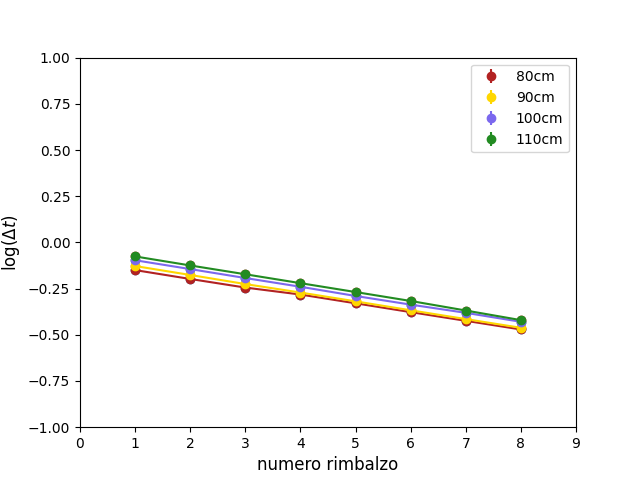
\includegraphics{Metodo2/computed_data/graficoLog_pallina4.png}
			} %close resize
		} %close centering
		\caption{Figura11:\(log\Delta t _{(n)}\) - pallina da golf su marmo}
	\end{figure}
	
	\noindent Abbiamo ricavato il coefficiente angolare di ciascuna delle 5 rette tramite il metodo dei minimi quadrati.
	
	\begin{figure}[!ht]
		\captionsetup{labelformat=empty}
		\makebox[1 \textwidth][c]{       %centering table
			\resizebox{0.7 \textwidth}{!}{   %resize table
				%%% Creator: Matplotlib, PGF backend
%%
%% To include the figure in your LaTeX document, write
%%   \input{<filename>.pgf}
%%
%% Make sure the required packages are loaded in your preamble
%%   \usepackage{pgf}
%%
%% and, on pdftex
%%   \usepackage[utf8]{inputenc}\DeclareUnicodeCharacter{2212}{-}
%%
%% or, on luatex and xetex
%%   \usepackage{unicode-math}
%%
%% Figures using additional raster images can only be included by \input if
%% they are in the same directory as the main LaTeX file. For loading figures
%% from other directories you can use the `import` package
%%   \usepackage{import}
%%
%% and then include the figures with
%%   \import{<path to file>}{<filename>.pgf}
%%
%% Matplotlib used the following preamble
%%   \usepackage{fontspec}
%%   \setmainfont{DejaVuSerif.ttf}[Path=C:/Users/giuly/AppData/Local/Programs/Python/Python39/Lib/site-packages/matplotlib/mpl-data/fonts/ttf/]
%%   \setsansfont{DejaVuSans.ttf}[Path=C:/Users/giuly/AppData/Local/Programs/Python/Python39/Lib/site-packages/matplotlib/mpl-data/fonts/ttf/]
%%   \setmonofont{DejaVuSansMono.ttf}[Path=C:/Users/giuly/AppData/Local/Programs/Python/Python39/Lib/site-packages/matplotlib/mpl-data/fonts/ttf/]
%%
\begingroup%
\makeatletter%
\begin{pgfpicture}%
\pgfpathrectangle{\pgfpointorigin}{\pgfqpoint{6.400000in}{4.800000in}}%
\pgfusepath{use as bounding box, clip}%
\begin{pgfscope}%
\pgfsetbuttcap%
\pgfsetmiterjoin%
\definecolor{currentfill}{rgb}{1.000000,1.000000,1.000000}%
\pgfsetfillcolor{currentfill}%
\pgfsetlinewidth{0.000000pt}%
\definecolor{currentstroke}{rgb}{1.000000,1.000000,1.000000}%
\pgfsetstrokecolor{currentstroke}%
\pgfsetdash{}{0pt}%
\pgfpathmoveto{\pgfqpoint{0.000000in}{0.000000in}}%
\pgfpathlineto{\pgfqpoint{6.400000in}{0.000000in}}%
\pgfpathlineto{\pgfqpoint{6.400000in}{4.800000in}}%
\pgfpathlineto{\pgfqpoint{0.000000in}{4.800000in}}%
\pgfpathclose%
\pgfusepath{fill}%
\end{pgfscope}%
\begin{pgfscope}%
\pgfsetbuttcap%
\pgfsetmiterjoin%
\definecolor{currentfill}{rgb}{1.000000,1.000000,1.000000}%
\pgfsetfillcolor{currentfill}%
\pgfsetlinewidth{0.000000pt}%
\definecolor{currentstroke}{rgb}{0.000000,0.000000,0.000000}%
\pgfsetstrokecolor{currentstroke}%
\pgfsetstrokeopacity{0.000000}%
\pgfsetdash{}{0pt}%
\pgfpathmoveto{\pgfqpoint{0.800000in}{0.528000in}}%
\pgfpathlineto{\pgfqpoint{5.760000in}{0.528000in}}%
\pgfpathlineto{\pgfqpoint{5.760000in}{4.224000in}}%
\pgfpathlineto{\pgfqpoint{0.800000in}{4.224000in}}%
\pgfpathclose%
\pgfusepath{fill}%
\end{pgfscope}%
\begin{pgfscope}%
\pgfpathrectangle{\pgfqpoint{0.800000in}{0.528000in}}{\pgfqpoint{4.960000in}{3.696000in}}%
\pgfusepath{clip}%
\pgfsetbuttcap%
\pgfsetmiterjoin%
\definecolor{currentfill}{rgb}{0.400000,0.803922,0.666667}%
\pgfsetfillcolor{currentfill}%
\pgfsetfillopacity{0.800000}%
\pgfsetlinewidth{0.000000pt}%
\definecolor{currentstroke}{rgb}{0.000000,0.000000,0.000000}%
\pgfsetstrokecolor{currentstroke}%
\pgfsetstrokeopacity{0.800000}%
\pgfsetdash{}{0pt}%
\pgfpathmoveto{\pgfqpoint{1.025455in}{0.528000in}}%
\pgfpathlineto{\pgfqpoint{1.401212in}{0.528000in}}%
\pgfpathlineto{\pgfqpoint{1.401212in}{0.848000in}}%
\pgfpathlineto{\pgfqpoint{1.025455in}{0.848000in}}%
\pgfpathclose%
\pgfusepath{fill}%
\end{pgfscope}%
\begin{pgfscope}%
\pgfpathrectangle{\pgfqpoint{0.800000in}{0.528000in}}{\pgfqpoint{4.960000in}{3.696000in}}%
\pgfusepath{clip}%
\pgfsetbuttcap%
\pgfsetmiterjoin%
\definecolor{currentfill}{rgb}{0.400000,0.803922,0.666667}%
\pgfsetfillcolor{currentfill}%
\pgfsetfillopacity{0.800000}%
\pgfsetlinewidth{0.000000pt}%
\definecolor{currentstroke}{rgb}{0.000000,0.000000,0.000000}%
\pgfsetstrokecolor{currentstroke}%
\pgfsetstrokeopacity{0.800000}%
\pgfsetdash{}{0pt}%
\pgfpathmoveto{\pgfqpoint{1.401212in}{0.528000in}}%
\pgfpathlineto{\pgfqpoint{1.776970in}{0.528000in}}%
\pgfpathlineto{\pgfqpoint{1.776970in}{0.848000in}}%
\pgfpathlineto{\pgfqpoint{1.401212in}{0.848000in}}%
\pgfpathclose%
\pgfusepath{fill}%
\end{pgfscope}%
\begin{pgfscope}%
\pgfpathrectangle{\pgfqpoint{0.800000in}{0.528000in}}{\pgfqpoint{4.960000in}{3.696000in}}%
\pgfusepath{clip}%
\pgfsetbuttcap%
\pgfsetmiterjoin%
\definecolor{currentfill}{rgb}{0.400000,0.803922,0.666667}%
\pgfsetfillcolor{currentfill}%
\pgfsetfillopacity{0.800000}%
\pgfsetlinewidth{0.000000pt}%
\definecolor{currentstroke}{rgb}{0.000000,0.000000,0.000000}%
\pgfsetstrokecolor{currentstroke}%
\pgfsetstrokeopacity{0.800000}%
\pgfsetdash{}{0pt}%
\pgfpathmoveto{\pgfqpoint{1.776970in}{0.528000in}}%
\pgfpathlineto{\pgfqpoint{2.152727in}{0.528000in}}%
\pgfpathlineto{\pgfqpoint{2.152727in}{1.168000in}}%
\pgfpathlineto{\pgfqpoint{1.776970in}{1.168000in}}%
\pgfpathclose%
\pgfusepath{fill}%
\end{pgfscope}%
\begin{pgfscope}%
\pgfpathrectangle{\pgfqpoint{0.800000in}{0.528000in}}{\pgfqpoint{4.960000in}{3.696000in}}%
\pgfusepath{clip}%
\pgfsetbuttcap%
\pgfsetmiterjoin%
\definecolor{currentfill}{rgb}{0.400000,0.803922,0.666667}%
\pgfsetfillcolor{currentfill}%
\pgfsetfillopacity{0.800000}%
\pgfsetlinewidth{0.000000pt}%
\definecolor{currentstroke}{rgb}{0.000000,0.000000,0.000000}%
\pgfsetstrokecolor{currentstroke}%
\pgfsetstrokeopacity{0.800000}%
\pgfsetdash{}{0pt}%
\pgfpathmoveto{\pgfqpoint{2.152727in}{0.528000in}}%
\pgfpathlineto{\pgfqpoint{2.528485in}{0.528000in}}%
\pgfpathlineto{\pgfqpoint{2.528485in}{1.968000in}}%
\pgfpathlineto{\pgfqpoint{2.152727in}{1.968000in}}%
\pgfpathclose%
\pgfusepath{fill}%
\end{pgfscope}%
\begin{pgfscope}%
\pgfpathrectangle{\pgfqpoint{0.800000in}{0.528000in}}{\pgfqpoint{4.960000in}{3.696000in}}%
\pgfusepath{clip}%
\pgfsetbuttcap%
\pgfsetmiterjoin%
\definecolor{currentfill}{rgb}{0.400000,0.803922,0.666667}%
\pgfsetfillcolor{currentfill}%
\pgfsetfillopacity{0.800000}%
\pgfsetlinewidth{0.000000pt}%
\definecolor{currentstroke}{rgb}{0.000000,0.000000,0.000000}%
\pgfsetstrokecolor{currentstroke}%
\pgfsetstrokeopacity{0.800000}%
\pgfsetdash{}{0pt}%
\pgfpathmoveto{\pgfqpoint{2.528485in}{0.528000in}}%
\pgfpathlineto{\pgfqpoint{2.904242in}{0.528000in}}%
\pgfpathlineto{\pgfqpoint{2.904242in}{2.448000in}}%
\pgfpathlineto{\pgfqpoint{2.528485in}{2.448000in}}%
\pgfpathclose%
\pgfusepath{fill}%
\end{pgfscope}%
\begin{pgfscope}%
\pgfpathrectangle{\pgfqpoint{0.800000in}{0.528000in}}{\pgfqpoint{4.960000in}{3.696000in}}%
\pgfusepath{clip}%
\pgfsetbuttcap%
\pgfsetmiterjoin%
\definecolor{currentfill}{rgb}{0.400000,0.803922,0.666667}%
\pgfsetfillcolor{currentfill}%
\pgfsetfillopacity{0.800000}%
\pgfsetlinewidth{0.000000pt}%
\definecolor{currentstroke}{rgb}{0.000000,0.000000,0.000000}%
\pgfsetstrokecolor{currentstroke}%
\pgfsetstrokeopacity{0.800000}%
\pgfsetdash{}{0pt}%
\pgfpathmoveto{\pgfqpoint{2.904242in}{0.528000in}}%
\pgfpathlineto{\pgfqpoint{3.280000in}{0.528000in}}%
\pgfpathlineto{\pgfqpoint{3.280000in}{4.048000in}}%
\pgfpathlineto{\pgfqpoint{2.904242in}{4.048000in}}%
\pgfpathclose%
\pgfusepath{fill}%
\end{pgfscope}%
\begin{pgfscope}%
\pgfpathrectangle{\pgfqpoint{0.800000in}{0.528000in}}{\pgfqpoint{4.960000in}{3.696000in}}%
\pgfusepath{clip}%
\pgfsetbuttcap%
\pgfsetmiterjoin%
\definecolor{currentfill}{rgb}{0.400000,0.803922,0.666667}%
\pgfsetfillcolor{currentfill}%
\pgfsetfillopacity{0.800000}%
\pgfsetlinewidth{0.000000pt}%
\definecolor{currentstroke}{rgb}{0.000000,0.000000,0.000000}%
\pgfsetstrokecolor{currentstroke}%
\pgfsetstrokeopacity{0.800000}%
\pgfsetdash{}{0pt}%
\pgfpathmoveto{\pgfqpoint{3.280000in}{0.528000in}}%
\pgfpathlineto{\pgfqpoint{3.655758in}{0.528000in}}%
\pgfpathlineto{\pgfqpoint{3.655758in}{3.248000in}}%
\pgfpathlineto{\pgfqpoint{3.280000in}{3.248000in}}%
\pgfpathclose%
\pgfusepath{fill}%
\end{pgfscope}%
\begin{pgfscope}%
\pgfpathrectangle{\pgfqpoint{0.800000in}{0.528000in}}{\pgfqpoint{4.960000in}{3.696000in}}%
\pgfusepath{clip}%
\pgfsetbuttcap%
\pgfsetmiterjoin%
\definecolor{currentfill}{rgb}{0.400000,0.803922,0.666667}%
\pgfsetfillcolor{currentfill}%
\pgfsetfillopacity{0.800000}%
\pgfsetlinewidth{0.000000pt}%
\definecolor{currentstroke}{rgb}{0.000000,0.000000,0.000000}%
\pgfsetstrokecolor{currentstroke}%
\pgfsetstrokeopacity{0.800000}%
\pgfsetdash{}{0pt}%
\pgfpathmoveto{\pgfqpoint{3.655758in}{0.528000in}}%
\pgfpathlineto{\pgfqpoint{4.031515in}{0.528000in}}%
\pgfpathlineto{\pgfqpoint{4.031515in}{3.248000in}}%
\pgfpathlineto{\pgfqpoint{3.655758in}{3.248000in}}%
\pgfpathclose%
\pgfusepath{fill}%
\end{pgfscope}%
\begin{pgfscope}%
\pgfpathrectangle{\pgfqpoint{0.800000in}{0.528000in}}{\pgfqpoint{4.960000in}{3.696000in}}%
\pgfusepath{clip}%
\pgfsetbuttcap%
\pgfsetmiterjoin%
\definecolor{currentfill}{rgb}{0.400000,0.803922,0.666667}%
\pgfsetfillcolor{currentfill}%
\pgfsetfillopacity{0.800000}%
\pgfsetlinewidth{0.000000pt}%
\definecolor{currentstroke}{rgb}{0.000000,0.000000,0.000000}%
\pgfsetstrokecolor{currentstroke}%
\pgfsetstrokeopacity{0.800000}%
\pgfsetdash{}{0pt}%
\pgfpathmoveto{\pgfqpoint{4.031515in}{0.528000in}}%
\pgfpathlineto{\pgfqpoint{4.407273in}{0.528000in}}%
\pgfpathlineto{\pgfqpoint{4.407273in}{1.968000in}}%
\pgfpathlineto{\pgfqpoint{4.031515in}{1.968000in}}%
\pgfpathclose%
\pgfusepath{fill}%
\end{pgfscope}%
\begin{pgfscope}%
\pgfpathrectangle{\pgfqpoint{0.800000in}{0.528000in}}{\pgfqpoint{4.960000in}{3.696000in}}%
\pgfusepath{clip}%
\pgfsetbuttcap%
\pgfsetmiterjoin%
\definecolor{currentfill}{rgb}{0.400000,0.803922,0.666667}%
\pgfsetfillcolor{currentfill}%
\pgfsetfillopacity{0.800000}%
\pgfsetlinewidth{0.000000pt}%
\definecolor{currentstroke}{rgb}{0.000000,0.000000,0.000000}%
\pgfsetstrokecolor{currentstroke}%
\pgfsetstrokeopacity{0.800000}%
\pgfsetdash{}{0pt}%
\pgfpathmoveto{\pgfqpoint{4.407273in}{0.528000in}}%
\pgfpathlineto{\pgfqpoint{4.783030in}{0.528000in}}%
\pgfpathlineto{\pgfqpoint{4.783030in}{1.168000in}}%
\pgfpathlineto{\pgfqpoint{4.407273in}{1.168000in}}%
\pgfpathclose%
\pgfusepath{fill}%
\end{pgfscope}%
\begin{pgfscope}%
\pgfpathrectangle{\pgfqpoint{0.800000in}{0.528000in}}{\pgfqpoint{4.960000in}{3.696000in}}%
\pgfusepath{clip}%
\pgfsetbuttcap%
\pgfsetmiterjoin%
\definecolor{currentfill}{rgb}{0.400000,0.803922,0.666667}%
\pgfsetfillcolor{currentfill}%
\pgfsetfillopacity{0.800000}%
\pgfsetlinewidth{0.000000pt}%
\definecolor{currentstroke}{rgb}{0.000000,0.000000,0.000000}%
\pgfsetstrokecolor{currentstroke}%
\pgfsetstrokeopacity{0.800000}%
\pgfsetdash{}{0pt}%
\pgfpathmoveto{\pgfqpoint{4.783030in}{0.528000in}}%
\pgfpathlineto{\pgfqpoint{5.158788in}{0.528000in}}%
\pgfpathlineto{\pgfqpoint{5.158788in}{0.688000in}}%
\pgfpathlineto{\pgfqpoint{4.783030in}{0.688000in}}%
\pgfpathclose%
\pgfusepath{fill}%
\end{pgfscope}%
\begin{pgfscope}%
\pgfpathrectangle{\pgfqpoint{0.800000in}{0.528000in}}{\pgfqpoint{4.960000in}{3.696000in}}%
\pgfusepath{clip}%
\pgfsetbuttcap%
\pgfsetmiterjoin%
\definecolor{currentfill}{rgb}{0.400000,0.803922,0.666667}%
\pgfsetfillcolor{currentfill}%
\pgfsetfillopacity{0.800000}%
\pgfsetlinewidth{0.000000pt}%
\definecolor{currentstroke}{rgb}{0.000000,0.000000,0.000000}%
\pgfsetstrokecolor{currentstroke}%
\pgfsetstrokeopacity{0.800000}%
\pgfsetdash{}{0pt}%
\pgfpathmoveto{\pgfqpoint{5.158788in}{0.528000in}}%
\pgfpathlineto{\pgfqpoint{5.534545in}{0.528000in}}%
\pgfpathlineto{\pgfqpoint{5.534545in}{0.688000in}}%
\pgfpathlineto{\pgfqpoint{5.158788in}{0.688000in}}%
\pgfpathclose%
\pgfusepath{fill}%
\end{pgfscope}%
\begin{pgfscope}%
\pgfsetbuttcap%
\pgfsetroundjoin%
\definecolor{currentfill}{rgb}{0.000000,0.000000,0.000000}%
\pgfsetfillcolor{currentfill}%
\pgfsetlinewidth{0.803000pt}%
\definecolor{currentstroke}{rgb}{0.000000,0.000000,0.000000}%
\pgfsetstrokecolor{currentstroke}%
\pgfsetdash{}{0pt}%
\pgfsys@defobject{currentmarker}{\pgfqpoint{0.000000in}{-0.048611in}}{\pgfqpoint{0.000000in}{0.000000in}}{%
\pgfpathmoveto{\pgfqpoint{0.000000in}{0.000000in}}%
\pgfpathlineto{\pgfqpoint{0.000000in}{-0.048611in}}%
\pgfusepath{stroke,fill}%
}%
\begin{pgfscope}%
\pgfsys@transformshift{1.025455in}{0.528000in}%
\pgfsys@useobject{currentmarker}{}%
\end{pgfscope}%
\end{pgfscope}%
\begin{pgfscope}%
\definecolor{textcolor}{rgb}{0.000000,0.000000,0.000000}%
\pgfsetstrokecolor{textcolor}%
\pgfsetfillcolor{textcolor}%
\pgftext[x=1.025455in,y=0.430778in,,top]{\color{textcolor}\sffamily\fontsize{10.000000}{12.000000}\selectfont 1.30}%
\end{pgfscope}%
\begin{pgfscope}%
\pgfsetbuttcap%
\pgfsetroundjoin%
\definecolor{currentfill}{rgb}{0.000000,0.000000,0.000000}%
\pgfsetfillcolor{currentfill}%
\pgfsetlinewidth{0.803000pt}%
\definecolor{currentstroke}{rgb}{0.000000,0.000000,0.000000}%
\pgfsetstrokecolor{currentstroke}%
\pgfsetdash{}{0pt}%
\pgfsys@defobject{currentmarker}{\pgfqpoint{0.000000in}{-0.048611in}}{\pgfqpoint{0.000000in}{0.000000in}}{%
\pgfpathmoveto{\pgfqpoint{0.000000in}{0.000000in}}%
\pgfpathlineto{\pgfqpoint{0.000000in}{-0.048611in}}%
\pgfusepath{stroke,fill}%
}%
\begin{pgfscope}%
\pgfsys@transformshift{1.589091in}{0.528000in}%
\pgfsys@useobject{currentmarker}{}%
\end{pgfscope}%
\end{pgfscope}%
\begin{pgfscope}%
\definecolor{textcolor}{rgb}{0.000000,0.000000,0.000000}%
\pgfsetstrokecolor{textcolor}%
\pgfsetfillcolor{textcolor}%
\pgftext[x=1.589091in,y=0.430778in,,top]{\color{textcolor}\sffamily\fontsize{10.000000}{12.000000}\selectfont 1.35}%
\end{pgfscope}%
\begin{pgfscope}%
\pgfsetbuttcap%
\pgfsetroundjoin%
\definecolor{currentfill}{rgb}{0.000000,0.000000,0.000000}%
\pgfsetfillcolor{currentfill}%
\pgfsetlinewidth{0.803000pt}%
\definecolor{currentstroke}{rgb}{0.000000,0.000000,0.000000}%
\pgfsetstrokecolor{currentstroke}%
\pgfsetdash{}{0pt}%
\pgfsys@defobject{currentmarker}{\pgfqpoint{0.000000in}{-0.048611in}}{\pgfqpoint{0.000000in}{0.000000in}}{%
\pgfpathmoveto{\pgfqpoint{0.000000in}{0.000000in}}%
\pgfpathlineto{\pgfqpoint{0.000000in}{-0.048611in}}%
\pgfusepath{stroke,fill}%
}%
\begin{pgfscope}%
\pgfsys@transformshift{2.152727in}{0.528000in}%
\pgfsys@useobject{currentmarker}{}%
\end{pgfscope}%
\end{pgfscope}%
\begin{pgfscope}%
\definecolor{textcolor}{rgb}{0.000000,0.000000,0.000000}%
\pgfsetstrokecolor{textcolor}%
\pgfsetfillcolor{textcolor}%
\pgftext[x=2.152727in,y=0.430778in,,top]{\color{textcolor}\sffamily\fontsize{10.000000}{12.000000}\selectfont 1.40}%
\end{pgfscope}%
\begin{pgfscope}%
\pgfsetbuttcap%
\pgfsetroundjoin%
\definecolor{currentfill}{rgb}{0.000000,0.000000,0.000000}%
\pgfsetfillcolor{currentfill}%
\pgfsetlinewidth{0.803000pt}%
\definecolor{currentstroke}{rgb}{0.000000,0.000000,0.000000}%
\pgfsetstrokecolor{currentstroke}%
\pgfsetdash{}{0pt}%
\pgfsys@defobject{currentmarker}{\pgfqpoint{0.000000in}{-0.048611in}}{\pgfqpoint{0.000000in}{0.000000in}}{%
\pgfpathmoveto{\pgfqpoint{0.000000in}{0.000000in}}%
\pgfpathlineto{\pgfqpoint{0.000000in}{-0.048611in}}%
\pgfusepath{stroke,fill}%
}%
\begin{pgfscope}%
\pgfsys@transformshift{2.716364in}{0.528000in}%
\pgfsys@useobject{currentmarker}{}%
\end{pgfscope}%
\end{pgfscope}%
\begin{pgfscope}%
\definecolor{textcolor}{rgb}{0.000000,0.000000,0.000000}%
\pgfsetstrokecolor{textcolor}%
\pgfsetfillcolor{textcolor}%
\pgftext[x=2.716364in,y=0.430778in,,top]{\color{textcolor}\sffamily\fontsize{10.000000}{12.000000}\selectfont 1.45}%
\end{pgfscope}%
\begin{pgfscope}%
\pgfsetbuttcap%
\pgfsetroundjoin%
\definecolor{currentfill}{rgb}{0.000000,0.000000,0.000000}%
\pgfsetfillcolor{currentfill}%
\pgfsetlinewidth{0.803000pt}%
\definecolor{currentstroke}{rgb}{0.000000,0.000000,0.000000}%
\pgfsetstrokecolor{currentstroke}%
\pgfsetdash{}{0pt}%
\pgfsys@defobject{currentmarker}{\pgfqpoint{0.000000in}{-0.048611in}}{\pgfqpoint{0.000000in}{0.000000in}}{%
\pgfpathmoveto{\pgfqpoint{0.000000in}{0.000000in}}%
\pgfpathlineto{\pgfqpoint{0.000000in}{-0.048611in}}%
\pgfusepath{stroke,fill}%
}%
\begin{pgfscope}%
\pgfsys@transformshift{3.280000in}{0.528000in}%
\pgfsys@useobject{currentmarker}{}%
\end{pgfscope}%
\end{pgfscope}%
\begin{pgfscope}%
\definecolor{textcolor}{rgb}{0.000000,0.000000,0.000000}%
\pgfsetstrokecolor{textcolor}%
\pgfsetfillcolor{textcolor}%
\pgftext[x=3.280000in,y=0.430778in,,top]{\color{textcolor}\sffamily\fontsize{10.000000}{12.000000}\selectfont 1.50}%
\end{pgfscope}%
\begin{pgfscope}%
\pgfsetbuttcap%
\pgfsetroundjoin%
\definecolor{currentfill}{rgb}{0.000000,0.000000,0.000000}%
\pgfsetfillcolor{currentfill}%
\pgfsetlinewidth{0.803000pt}%
\definecolor{currentstroke}{rgb}{0.000000,0.000000,0.000000}%
\pgfsetstrokecolor{currentstroke}%
\pgfsetdash{}{0pt}%
\pgfsys@defobject{currentmarker}{\pgfqpoint{0.000000in}{-0.048611in}}{\pgfqpoint{0.000000in}{0.000000in}}{%
\pgfpathmoveto{\pgfqpoint{0.000000in}{0.000000in}}%
\pgfpathlineto{\pgfqpoint{0.000000in}{-0.048611in}}%
\pgfusepath{stroke,fill}%
}%
\begin{pgfscope}%
\pgfsys@transformshift{3.843636in}{0.528000in}%
\pgfsys@useobject{currentmarker}{}%
\end{pgfscope}%
\end{pgfscope}%
\begin{pgfscope}%
\definecolor{textcolor}{rgb}{0.000000,0.000000,0.000000}%
\pgfsetstrokecolor{textcolor}%
\pgfsetfillcolor{textcolor}%
\pgftext[x=3.843636in,y=0.430778in,,top]{\color{textcolor}\sffamily\fontsize{10.000000}{12.000000}\selectfont 1.55}%
\end{pgfscope}%
\begin{pgfscope}%
\pgfsetbuttcap%
\pgfsetroundjoin%
\definecolor{currentfill}{rgb}{0.000000,0.000000,0.000000}%
\pgfsetfillcolor{currentfill}%
\pgfsetlinewidth{0.803000pt}%
\definecolor{currentstroke}{rgb}{0.000000,0.000000,0.000000}%
\pgfsetstrokecolor{currentstroke}%
\pgfsetdash{}{0pt}%
\pgfsys@defobject{currentmarker}{\pgfqpoint{0.000000in}{-0.048611in}}{\pgfqpoint{0.000000in}{0.000000in}}{%
\pgfpathmoveto{\pgfqpoint{0.000000in}{0.000000in}}%
\pgfpathlineto{\pgfqpoint{0.000000in}{-0.048611in}}%
\pgfusepath{stroke,fill}%
}%
\begin{pgfscope}%
\pgfsys@transformshift{4.407273in}{0.528000in}%
\pgfsys@useobject{currentmarker}{}%
\end{pgfscope}%
\end{pgfscope}%
\begin{pgfscope}%
\definecolor{textcolor}{rgb}{0.000000,0.000000,0.000000}%
\pgfsetstrokecolor{textcolor}%
\pgfsetfillcolor{textcolor}%
\pgftext[x=4.407273in,y=0.430778in,,top]{\color{textcolor}\sffamily\fontsize{10.000000}{12.000000}\selectfont 1.60}%
\end{pgfscope}%
\begin{pgfscope}%
\pgfsetbuttcap%
\pgfsetroundjoin%
\definecolor{currentfill}{rgb}{0.000000,0.000000,0.000000}%
\pgfsetfillcolor{currentfill}%
\pgfsetlinewidth{0.803000pt}%
\definecolor{currentstroke}{rgb}{0.000000,0.000000,0.000000}%
\pgfsetstrokecolor{currentstroke}%
\pgfsetdash{}{0pt}%
\pgfsys@defobject{currentmarker}{\pgfqpoint{0.000000in}{-0.048611in}}{\pgfqpoint{0.000000in}{0.000000in}}{%
\pgfpathmoveto{\pgfqpoint{0.000000in}{0.000000in}}%
\pgfpathlineto{\pgfqpoint{0.000000in}{-0.048611in}}%
\pgfusepath{stroke,fill}%
}%
\begin{pgfscope}%
\pgfsys@transformshift{4.970909in}{0.528000in}%
\pgfsys@useobject{currentmarker}{}%
\end{pgfscope}%
\end{pgfscope}%
\begin{pgfscope}%
\definecolor{textcolor}{rgb}{0.000000,0.000000,0.000000}%
\pgfsetstrokecolor{textcolor}%
\pgfsetfillcolor{textcolor}%
\pgftext[x=4.970909in,y=0.430778in,,top]{\color{textcolor}\sffamily\fontsize{10.000000}{12.000000}\selectfont 1.65}%
\end{pgfscope}%
\begin{pgfscope}%
\pgfsetbuttcap%
\pgfsetroundjoin%
\definecolor{currentfill}{rgb}{0.000000,0.000000,0.000000}%
\pgfsetfillcolor{currentfill}%
\pgfsetlinewidth{0.803000pt}%
\definecolor{currentstroke}{rgb}{0.000000,0.000000,0.000000}%
\pgfsetstrokecolor{currentstroke}%
\pgfsetdash{}{0pt}%
\pgfsys@defobject{currentmarker}{\pgfqpoint{0.000000in}{-0.048611in}}{\pgfqpoint{0.000000in}{0.000000in}}{%
\pgfpathmoveto{\pgfqpoint{0.000000in}{0.000000in}}%
\pgfpathlineto{\pgfqpoint{0.000000in}{-0.048611in}}%
\pgfusepath{stroke,fill}%
}%
\begin{pgfscope}%
\pgfsys@transformshift{5.534545in}{0.528000in}%
\pgfsys@useobject{currentmarker}{}%
\end{pgfscope}%
\end{pgfscope}%
\begin{pgfscope}%
\definecolor{textcolor}{rgb}{0.000000,0.000000,0.000000}%
\pgfsetstrokecolor{textcolor}%
\pgfsetfillcolor{textcolor}%
\pgftext[x=5.534545in,y=0.430778in,,top]{\color{textcolor}\sffamily\fontsize{10.000000}{12.000000}\selectfont 1.70}%
\end{pgfscope}%
\begin{pgfscope}%
\definecolor{textcolor}{rgb}{0.000000,0.000000,0.000000}%
\pgfsetstrokecolor{textcolor}%
\pgfsetfillcolor{textcolor}%
\pgftext[x=3.280000in,y=0.240809in,,top]{\color{textcolor}\sffamily\fontsize{10.000000}{12.000000}\selectfont \(\displaystyle x_k\) (s)}%
\end{pgfscope}%
\begin{pgfscope}%
\pgfsetbuttcap%
\pgfsetroundjoin%
\definecolor{currentfill}{rgb}{0.000000,0.000000,0.000000}%
\pgfsetfillcolor{currentfill}%
\pgfsetlinewidth{0.803000pt}%
\definecolor{currentstroke}{rgb}{0.000000,0.000000,0.000000}%
\pgfsetstrokecolor{currentstroke}%
\pgfsetdash{}{0pt}%
\pgfsys@defobject{currentmarker}{\pgfqpoint{-0.048611in}{0.000000in}}{\pgfqpoint{-0.000000in}{0.000000in}}{%
\pgfpathmoveto{\pgfqpoint{-0.000000in}{0.000000in}}%
\pgfpathlineto{\pgfqpoint{-0.048611in}{0.000000in}}%
\pgfusepath{stroke,fill}%
}%
\begin{pgfscope}%
\pgfsys@transformshift{0.800000in}{0.528000in}%
\pgfsys@useobject{currentmarker}{}%
\end{pgfscope}%
\end{pgfscope}%
\begin{pgfscope}%
\definecolor{textcolor}{rgb}{0.000000,0.000000,0.000000}%
\pgfsetstrokecolor{textcolor}%
\pgfsetfillcolor{textcolor}%
\pgftext[x=0.614412in, y=0.475238in, left, base]{\color{textcolor}\sffamily\fontsize{10.000000}{12.000000}\selectfont 0}%
\end{pgfscope}%
\begin{pgfscope}%
\pgfsetbuttcap%
\pgfsetroundjoin%
\definecolor{currentfill}{rgb}{0.000000,0.000000,0.000000}%
\pgfsetfillcolor{currentfill}%
\pgfsetlinewidth{0.803000pt}%
\definecolor{currentstroke}{rgb}{0.000000,0.000000,0.000000}%
\pgfsetstrokecolor{currentstroke}%
\pgfsetdash{}{0pt}%
\pgfsys@defobject{currentmarker}{\pgfqpoint{-0.048611in}{0.000000in}}{\pgfqpoint{-0.000000in}{0.000000in}}{%
\pgfpathmoveto{\pgfqpoint{-0.000000in}{0.000000in}}%
\pgfpathlineto{\pgfqpoint{-0.048611in}{0.000000in}}%
\pgfusepath{stroke,fill}%
}%
\begin{pgfscope}%
\pgfsys@transformshift{0.800000in}{1.061333in}%
\pgfsys@useobject{currentmarker}{}%
\end{pgfscope}%
\end{pgfscope}%
\begin{pgfscope}%
\definecolor{textcolor}{rgb}{0.000000,0.000000,0.000000}%
\pgfsetstrokecolor{textcolor}%
\pgfsetfillcolor{textcolor}%
\pgftext[x=0.614412in, y=1.008572in, left, base]{\color{textcolor}\sffamily\fontsize{10.000000}{12.000000}\selectfont 1}%
\end{pgfscope}%
\begin{pgfscope}%
\pgfsetbuttcap%
\pgfsetroundjoin%
\definecolor{currentfill}{rgb}{0.000000,0.000000,0.000000}%
\pgfsetfillcolor{currentfill}%
\pgfsetlinewidth{0.803000pt}%
\definecolor{currentstroke}{rgb}{0.000000,0.000000,0.000000}%
\pgfsetstrokecolor{currentstroke}%
\pgfsetdash{}{0pt}%
\pgfsys@defobject{currentmarker}{\pgfqpoint{-0.048611in}{0.000000in}}{\pgfqpoint{-0.000000in}{0.000000in}}{%
\pgfpathmoveto{\pgfqpoint{-0.000000in}{0.000000in}}%
\pgfpathlineto{\pgfqpoint{-0.048611in}{0.000000in}}%
\pgfusepath{stroke,fill}%
}%
\begin{pgfscope}%
\pgfsys@transformshift{0.800000in}{1.594667in}%
\pgfsys@useobject{currentmarker}{}%
\end{pgfscope}%
\end{pgfscope}%
\begin{pgfscope}%
\definecolor{textcolor}{rgb}{0.000000,0.000000,0.000000}%
\pgfsetstrokecolor{textcolor}%
\pgfsetfillcolor{textcolor}%
\pgftext[x=0.614412in, y=1.541905in, left, base]{\color{textcolor}\sffamily\fontsize{10.000000}{12.000000}\selectfont 2}%
\end{pgfscope}%
\begin{pgfscope}%
\pgfsetbuttcap%
\pgfsetroundjoin%
\definecolor{currentfill}{rgb}{0.000000,0.000000,0.000000}%
\pgfsetfillcolor{currentfill}%
\pgfsetlinewidth{0.803000pt}%
\definecolor{currentstroke}{rgb}{0.000000,0.000000,0.000000}%
\pgfsetstrokecolor{currentstroke}%
\pgfsetdash{}{0pt}%
\pgfsys@defobject{currentmarker}{\pgfqpoint{-0.048611in}{0.000000in}}{\pgfqpoint{-0.000000in}{0.000000in}}{%
\pgfpathmoveto{\pgfqpoint{-0.000000in}{0.000000in}}%
\pgfpathlineto{\pgfqpoint{-0.048611in}{0.000000in}}%
\pgfusepath{stroke,fill}%
}%
\begin{pgfscope}%
\pgfsys@transformshift{0.800000in}{2.128000in}%
\pgfsys@useobject{currentmarker}{}%
\end{pgfscope}%
\end{pgfscope}%
\begin{pgfscope}%
\definecolor{textcolor}{rgb}{0.000000,0.000000,0.000000}%
\pgfsetstrokecolor{textcolor}%
\pgfsetfillcolor{textcolor}%
\pgftext[x=0.614412in, y=2.075238in, left, base]{\color{textcolor}\sffamily\fontsize{10.000000}{12.000000}\selectfont 3}%
\end{pgfscope}%
\begin{pgfscope}%
\pgfsetbuttcap%
\pgfsetroundjoin%
\definecolor{currentfill}{rgb}{0.000000,0.000000,0.000000}%
\pgfsetfillcolor{currentfill}%
\pgfsetlinewidth{0.803000pt}%
\definecolor{currentstroke}{rgb}{0.000000,0.000000,0.000000}%
\pgfsetstrokecolor{currentstroke}%
\pgfsetdash{}{0pt}%
\pgfsys@defobject{currentmarker}{\pgfqpoint{-0.048611in}{0.000000in}}{\pgfqpoint{-0.000000in}{0.000000in}}{%
\pgfpathmoveto{\pgfqpoint{-0.000000in}{0.000000in}}%
\pgfpathlineto{\pgfqpoint{-0.048611in}{0.000000in}}%
\pgfusepath{stroke,fill}%
}%
\begin{pgfscope}%
\pgfsys@transformshift{0.800000in}{2.661333in}%
\pgfsys@useobject{currentmarker}{}%
\end{pgfscope}%
\end{pgfscope}%
\begin{pgfscope}%
\definecolor{textcolor}{rgb}{0.000000,0.000000,0.000000}%
\pgfsetstrokecolor{textcolor}%
\pgfsetfillcolor{textcolor}%
\pgftext[x=0.614412in, y=2.608572in, left, base]{\color{textcolor}\sffamily\fontsize{10.000000}{12.000000}\selectfont 4}%
\end{pgfscope}%
\begin{pgfscope}%
\pgfsetbuttcap%
\pgfsetroundjoin%
\definecolor{currentfill}{rgb}{0.000000,0.000000,0.000000}%
\pgfsetfillcolor{currentfill}%
\pgfsetlinewidth{0.803000pt}%
\definecolor{currentstroke}{rgb}{0.000000,0.000000,0.000000}%
\pgfsetstrokecolor{currentstroke}%
\pgfsetdash{}{0pt}%
\pgfsys@defobject{currentmarker}{\pgfqpoint{-0.048611in}{0.000000in}}{\pgfqpoint{-0.000000in}{0.000000in}}{%
\pgfpathmoveto{\pgfqpoint{-0.000000in}{0.000000in}}%
\pgfpathlineto{\pgfqpoint{-0.048611in}{0.000000in}}%
\pgfusepath{stroke,fill}%
}%
\begin{pgfscope}%
\pgfsys@transformshift{0.800000in}{3.194667in}%
\pgfsys@useobject{currentmarker}{}%
\end{pgfscope}%
\end{pgfscope}%
\begin{pgfscope}%
\definecolor{textcolor}{rgb}{0.000000,0.000000,0.000000}%
\pgfsetstrokecolor{textcolor}%
\pgfsetfillcolor{textcolor}%
\pgftext[x=0.614412in, y=3.141905in, left, base]{\color{textcolor}\sffamily\fontsize{10.000000}{12.000000}\selectfont 5}%
\end{pgfscope}%
\begin{pgfscope}%
\pgfsetbuttcap%
\pgfsetroundjoin%
\definecolor{currentfill}{rgb}{0.000000,0.000000,0.000000}%
\pgfsetfillcolor{currentfill}%
\pgfsetlinewidth{0.803000pt}%
\definecolor{currentstroke}{rgb}{0.000000,0.000000,0.000000}%
\pgfsetstrokecolor{currentstroke}%
\pgfsetdash{}{0pt}%
\pgfsys@defobject{currentmarker}{\pgfqpoint{-0.048611in}{0.000000in}}{\pgfqpoint{-0.000000in}{0.000000in}}{%
\pgfpathmoveto{\pgfqpoint{-0.000000in}{0.000000in}}%
\pgfpathlineto{\pgfqpoint{-0.048611in}{0.000000in}}%
\pgfusepath{stroke,fill}%
}%
\begin{pgfscope}%
\pgfsys@transformshift{0.800000in}{3.728000in}%
\pgfsys@useobject{currentmarker}{}%
\end{pgfscope}%
\end{pgfscope}%
\begin{pgfscope}%
\definecolor{textcolor}{rgb}{0.000000,0.000000,0.000000}%
\pgfsetstrokecolor{textcolor}%
\pgfsetfillcolor{textcolor}%
\pgftext[x=0.614412in, y=3.675238in, left, base]{\color{textcolor}\sffamily\fontsize{10.000000}{12.000000}\selectfont 6}%
\end{pgfscope}%
\begin{pgfscope}%
\definecolor{textcolor}{rgb}{0.000000,0.000000,0.000000}%
\pgfsetstrokecolor{textcolor}%
\pgfsetfillcolor{textcolor}%
\pgftext[x=0.558857in,y=2.376000in,,bottom,rotate=90.000000]{\color{textcolor}\sffamily\fontsize{10.000000}{12.000000}\selectfont Densità di Frequenza}%
\end{pgfscope}%
\begin{pgfscope}%
\pgfpathrectangle{\pgfqpoint{0.800000in}{0.528000in}}{\pgfqpoint{4.960000in}{3.696000in}}%
\pgfusepath{clip}%
\pgfsetrectcap%
\pgfsetroundjoin%
\pgfsetlinewidth{1.505625pt}%
\definecolor{currentstroke}{rgb}{1.000000,0.549020,0.000000}%
\pgfsetstrokecolor{currentstroke}%
\pgfsetdash{}{0pt}%
\pgfpathmoveto{\pgfqpoint{1.025455in}{0.574044in}}%
\pgfpathlineto{\pgfqpoint{1.117477in}{0.593003in}}%
\pgfpathlineto{\pgfqpoint{1.209499in}{0.618431in}}%
\pgfpathlineto{\pgfqpoint{1.301521in}{0.651974in}}%
\pgfpathlineto{\pgfqpoint{1.393544in}{0.695485in}}%
\pgfpathlineto{\pgfqpoint{1.485566in}{0.750973in}}%
\pgfpathlineto{\pgfqpoint{1.577588in}{0.820521in}}%
\pgfpathlineto{\pgfqpoint{1.669610in}{0.906175in}}%
\pgfpathlineto{\pgfqpoint{1.761633in}{1.009791in}}%
\pgfpathlineto{\pgfqpoint{1.853655in}{1.132860in}}%
\pgfpathlineto{\pgfqpoint{1.945677in}{1.276309in}}%
\pgfpathlineto{\pgfqpoint{2.037699in}{1.440300in}}%
\pgfpathlineto{\pgfqpoint{2.129722in}{1.624034in}}%
\pgfpathlineto{\pgfqpoint{2.221744in}{1.825600in}}%
\pgfpathlineto{\pgfqpoint{2.313766in}{2.041867in}}%
\pgfpathlineto{\pgfqpoint{2.405788in}{2.268464in}}%
\pgfpathlineto{\pgfqpoint{2.497811in}{2.499842in}}%
\pgfpathlineto{\pgfqpoint{2.589833in}{2.729454in}}%
\pgfpathlineto{\pgfqpoint{2.681855in}{2.950017in}}%
\pgfpathlineto{\pgfqpoint{2.773878in}{3.153881in}}%
\pgfpathlineto{\pgfqpoint{2.865900in}{3.333452in}}%
\pgfpathlineto{\pgfqpoint{2.957922in}{3.481663in}}%
\pgfpathlineto{\pgfqpoint{3.049944in}{3.592427in}}%
\pgfpathlineto{\pgfqpoint{3.141967in}{3.661053in}}%
\pgfpathlineto{\pgfqpoint{3.233989in}{3.684577in}}%
\pgfpathlineto{\pgfqpoint{3.326011in}{3.661972in}}%
\pgfpathlineto{\pgfqpoint{3.418033in}{3.594225in}}%
\pgfpathlineto{\pgfqpoint{3.510056in}{3.484264in}}%
\pgfpathlineto{\pgfqpoint{3.602078in}{3.336746in}}%
\pgfpathlineto{\pgfqpoint{3.694100in}{3.157735in}}%
\pgfpathlineto{\pgfqpoint{3.786122in}{2.954284in}}%
\pgfpathlineto{\pgfqpoint{3.878145in}{2.733979in}}%
\pgfpathlineto{\pgfqpoint{3.970167in}{2.504475in}}%
\pgfpathlineto{\pgfqpoint{4.062189in}{2.273065in}}%
\pgfpathlineto{\pgfqpoint{4.154212in}{2.046315in}}%
\pgfpathlineto{\pgfqpoint{4.246234in}{1.829794in}}%
\pgfpathlineto{\pgfqpoint{4.338256in}{1.627899in}}%
\pgfpathlineto{\pgfqpoint{4.430278in}{1.443785in}}%
\pgfpathlineto{\pgfqpoint{4.522301in}{1.279389in}}%
\pgfpathlineto{\pgfqpoint{4.614323in}{1.135527in}}%
\pgfpathlineto{\pgfqpoint{4.706345in}{1.012058in}}%
\pgfpathlineto{\pgfqpoint{4.798367in}{0.908066in}}%
\pgfpathlineto{\pgfqpoint{4.890390in}{0.822070in}}%
\pgfpathlineto{\pgfqpoint{4.982412in}{0.752219in}}%
\pgfpathlineto{\pgfqpoint{5.074434in}{0.696471in}}%
\pgfpathlineto{\pgfqpoint{5.166456in}{0.652740in}}%
\pgfpathlineto{\pgfqpoint{5.258479in}{0.619016in}}%
\pgfpathlineto{\pgfqpoint{5.350501in}{0.593443in}}%
\pgfpathlineto{\pgfqpoint{5.442523in}{0.574370in}}%
\pgfpathlineto{\pgfqpoint{5.534545in}{0.560377in}}%
\pgfusepath{stroke}%
\end{pgfscope}%
\begin{pgfscope}%
\pgfsetrectcap%
\pgfsetmiterjoin%
\pgfsetlinewidth{0.803000pt}%
\definecolor{currentstroke}{rgb}{0.000000,0.000000,0.000000}%
\pgfsetstrokecolor{currentstroke}%
\pgfsetdash{}{0pt}%
\pgfpathmoveto{\pgfqpoint{0.800000in}{0.528000in}}%
\pgfpathlineto{\pgfqpoint{0.800000in}{4.224000in}}%
\pgfusepath{stroke}%
\end{pgfscope}%
\begin{pgfscope}%
\pgfsetrectcap%
\pgfsetmiterjoin%
\pgfsetlinewidth{0.803000pt}%
\definecolor{currentstroke}{rgb}{0.000000,0.000000,0.000000}%
\pgfsetstrokecolor{currentstroke}%
\pgfsetdash{}{0pt}%
\pgfpathmoveto{\pgfqpoint{5.760000in}{0.528000in}}%
\pgfpathlineto{\pgfqpoint{5.760000in}{4.224000in}}%
\pgfusepath{stroke}%
\end{pgfscope}%
\begin{pgfscope}%
\pgfsetrectcap%
\pgfsetmiterjoin%
\pgfsetlinewidth{0.803000pt}%
\definecolor{currentstroke}{rgb}{0.000000,0.000000,0.000000}%
\pgfsetstrokecolor{currentstroke}%
\pgfsetdash{}{0pt}%
\pgfpathmoveto{\pgfqpoint{0.800000in}{0.528000in}}%
\pgfpathlineto{\pgfqpoint{5.760000in}{0.528000in}}%
\pgfusepath{stroke}%
\end{pgfscope}%
\begin{pgfscope}%
\pgfsetrectcap%
\pgfsetmiterjoin%
\pgfsetlinewidth{0.803000pt}%
\definecolor{currentstroke}{rgb}{0.000000,0.000000,0.000000}%
\pgfsetstrokecolor{currentstroke}%
\pgfsetdash{}{0pt}%
\pgfpathmoveto{\pgfqpoint{0.800000in}{4.224000in}}%
\pgfpathlineto{\pgfqpoint{5.760000in}{4.224000in}}%
\pgfusepath{stroke}%
\end{pgfscope}%
\begin{pgfscope}%
\pgfsetbuttcap%
\pgfsetmiterjoin%
\definecolor{currentfill}{rgb}{1.000000,1.000000,1.000000}%
\pgfsetfillcolor{currentfill}%
\pgfsetfillopacity{0.800000}%
\pgfsetlinewidth{1.003750pt}%
\definecolor{currentstroke}{rgb}{0.800000,0.800000,0.800000}%
\pgfsetstrokecolor{currentstroke}%
\pgfsetstrokeopacity{0.800000}%
\pgfsetdash{}{0pt}%
\pgfpathmoveto{\pgfqpoint{4.613473in}{3.690899in}}%
\pgfpathlineto{\pgfqpoint{5.662778in}{3.690899in}}%
\pgfpathquadraticcurveto{\pgfqpoint{5.690556in}{3.690899in}}{\pgfqpoint{5.690556in}{3.718677in}}%
\pgfpathlineto{\pgfqpoint{5.690556in}{4.126778in}}%
\pgfpathquadraticcurveto{\pgfqpoint{5.690556in}{4.154556in}}{\pgfqpoint{5.662778in}{4.154556in}}%
\pgfpathlineto{\pgfqpoint{4.613473in}{4.154556in}}%
\pgfpathquadraticcurveto{\pgfqpoint{4.585695in}{4.154556in}}{\pgfqpoint{4.585695in}{4.126778in}}%
\pgfpathlineto{\pgfqpoint{4.585695in}{3.718677in}}%
\pgfpathquadraticcurveto{\pgfqpoint{4.585695in}{3.690899in}}{\pgfqpoint{4.613473in}{3.690899in}}%
\pgfpathclose%
\pgfusepath{stroke,fill}%
\end{pgfscope}%
\begin{pgfscope}%
\pgfsetrectcap%
\pgfsetroundjoin%
\pgfsetlinewidth{1.505625pt}%
\definecolor{currentstroke}{rgb}{1.000000,0.549020,0.000000}%
\pgfsetstrokecolor{currentstroke}%
\pgfsetdash{}{0pt}%
\pgfpathmoveto{\pgfqpoint{4.641251in}{4.033645in}}%
\pgfpathlineto{\pgfqpoint{4.919029in}{4.033645in}}%
\pgfusepath{stroke}%
\end{pgfscope}%
\begin{pgfscope}%
\definecolor{textcolor}{rgb}{0.000000,0.000000,0.000000}%
\pgfsetstrokecolor{textcolor}%
\pgfsetfillcolor{textcolor}%
\pgftext[x=5.030140in,y=3.985034in,left,base]{\color{textcolor}\sffamily\fontsize{10.000000}{12.000000}\selectfont \(\displaystyle G(x;\bar{T},\sigma)\)}%
\end{pgfscope}%
\begin{pgfscope}%
\pgfsetbuttcap%
\pgfsetmiterjoin%
\definecolor{currentfill}{rgb}{0.400000,0.803922,0.666667}%
\pgfsetfillcolor{currentfill}%
\pgfsetfillopacity{0.800000}%
\pgfsetlinewidth{0.000000pt}%
\definecolor{currentstroke}{rgb}{0.000000,0.000000,0.000000}%
\pgfsetstrokecolor{currentstroke}%
\pgfsetstrokeopacity{0.800000}%
\pgfsetdash{}{0pt}%
\pgfpathmoveto{\pgfqpoint{4.641251in}{3.775344in}}%
\pgfpathlineto{\pgfqpoint{4.919029in}{3.775344in}}%
\pgfpathlineto{\pgfqpoint{4.919029in}{3.872567in}}%
\pgfpathlineto{\pgfqpoint{4.641251in}{3.872567in}}%
\pgfpathclose%
\pgfusepath{fill}%
\end{pgfscope}%
\begin{pgfscope}%
\definecolor{textcolor}{rgb}{0.000000,0.000000,0.000000}%
\pgfsetstrokecolor{textcolor}%
\pgfsetfillcolor{textcolor}%
\pgftext[x=5.030140in,y=3.775344in,left,base]{\color{textcolor}\sffamily\fontsize{10.000000}{12.000000}\selectfont data}%
\end{pgfscope}%
\end{pgfpicture}%
\makeatother%
\endgroup%

				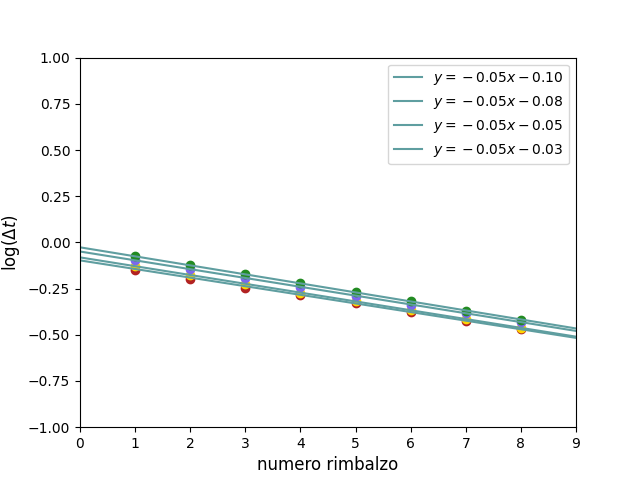
\includegraphics{Metodo2/computed_data/graficoLog_interpolato_pallina4.png}
			} %close resize
		} %close centering
		\caption{ Figura12: \(log\Delta t _{(n)}\) - pallina da golf - interpolazione}
	\end{figure}
	
	\noindent Così facendo si ottengono 5 stime del coefficiente di restituzione che possono essere combinate in una media pesata come \(\bar{e_{v}} = \frac{\sum\frac{e_{vi}}{\sigma_{i}}}{\sum\frac{1}{\sigma _{i}}}\).
	
	\[\begin{matrix}
		$80cm:$ &$\(B=-0.047\pm 0.001\rightarrow\)$& $\( ev= 0.8983\pm0.0024\)$ &  \\ 
		$90cm:$ & $\(B=-0.048\pm0.002\)$&$\(ev = 0.896\pm0.004\)$ &  \\ 
		$100cm:$ & $\(B=-0.048\pm 0.0007\)$& $\(ev =  0.8959\pm0.0014\)$ & $\(\qquad \Rightarrow \quad \bar{e_{v}} =0.8952 \pm 0.0009\)$\\ 
		$110cm:$ &$\(B=-0.049\pm 0.0006\)$& $\(ev = 0.8938\pm0.0013\)$ &  
	\end{matrix}\]
	dove \(e_{v}= 10^{B}\), \(\sigma_{ev} = 10^{B}ln(10)\sigma_{B}\) e l'incertezza sulla media pesata è \(\sigma _{media}=\sqrt{\frac{1}{\sum \frac{1}{\sigma _{i}}}}\). Notiamo che questa stima è molto più precisa di quella ottenuta con il metodo 1.
	
	\[t = \frac{ \left |ev_{metodo1}  - ev_{metodo2} \right |}{\sqrt{\sigma_{1}^{2}+ \sigma_{2}^{2}}} =  4,6 \]
\noindent \(\rightarrow\) la probabilità che la differenza sia dovuta solo ad errori casuali è inferiore al 0.3\(\%\).
\end{document}
	
\end{document}